% This LaTeX document needs to be compiled with XeLaTeX.
\documentclass[10pt]{article}
\usepackage[utf8]{inputenc}
\usepackage{ucharclasses}
\usepackage{amsmath}
\usepackage{amsfonts}
\usepackage{amssymb}
\usepackage[version=4]{mhchem}
\usepackage{stmaryrd}
\usepackage{caption}
\usepackage{graphicx}
\usepackage[export]{adjustbox}
\graphicspath{ {./images/} }
\usepackage{multirow}
\usepackage{underscore}
\usepackage{hyperref}
\hypersetup{colorlinks=true, linkcolor=blue, filecolor=magenta, urlcolor=cyan,}
\urlstyle{same}
\usepackage[fallback]{xeCJK}
\usepackage{polyglossia}
\usepackage{fontspec}
\IfFontExistsTF{Noto Serif CJK JP}
{\setCJKmainfont{Noto Serif CJK JP}}
{\IfFontExistsTF{STSong}
  {\setCJKmainfont{STSong}}
  {\IfFontExistsTF{Droid Sans Fallback}
    {\setCJKmainfont{Droid Sans Fallback}}
    {\setCJKmainfont{SimSun}}
}}

\setmainlanguage{english}
\setotherlanguages{polish, swedish, thai}
\IfFontExistsTF{Noto Serif Thai}
{\newfontfamily\thaifont{Noto Serif Thai}}
{\IfFontExistsTF{Thonburi}
  {\newfontfamily\thaifont{Thonburi}}
  {\IfFontExistsTF{FreeSerif}
    {\newfontfamily\thaifont{FreeSerif}}
    {\IfFontExistsTF{Tahoma}
      {\newfontfamily\thaifont{Tahoma}}
      {\newfontfamily\thaifont{Arial Unicode MS}}
}}}
\IfFontExistsTF{Noto Serif Gujarati}
{\newfontfamily\gujaratifont{Noto Serif Gujarati}}
{\IfFontExistsTF{Kohinoor Gujarati}
  {\newfontfamily\gujaratifont{Kohinoor Gujarati}}
  {\IfFontExistsTF{Gujarati MT}
    {\newfontfamily\gujaratifont{Gujarati MT}}
    {\IfFontExistsTF{Lohit Gujarati}
      {\newfontfamily\gujaratifont{Lohit Gujarati}}
      {\IfFontExistsTF{FreeSerif}
        {\newfontfamily\gujaratifont{FreeSerif}}
        {\newfontfamily\gujaratifont{Arial Unicode MS}}
}}}}
\IfFontExistsTF{CMU Serif}
{\newfontfamily\lgcfont{CMU Serif}}
{\IfFontExistsTF{DejaVu Sans}
  {\newfontfamily\lgcfont{DejaVu Sans}}
  {\newfontfamily\lgcfont{Georgia}}
}
\setDefaultTransitions{\lgcfont}{}
\setTransitionsFor{Thai}{\thaifont}{\lgcfont}
\setTransitionsFor{Gujarati}{\gujaratifont}{\rmfamily}

\title{Luang Grammar and Phonology Sketch }

\author{a. au-plinu\\
1s-do not know\\
'I do not know.'\\
b. au-plinu-a\\
1s-do not know-OBJ\\
'I do not know it.'\\
c. au-plinu nan-ni\\
1s do not know name-his\\
'I do not know his name.'\\
d. au-plinu wali-a\\
1s-do not know-OBJ\\
'I do not know it either.'}
\date{}


%New command to display footnote whose markers will always be hidden
\let\svthefootnote\thefootnote
\newcommand\blfootnotetext[1]{%
  \let\thefootnote\relax\footnote{#1}%
  \addtocounter{footnote}{-1}%
  \let\thefootnote\svthefootnote%
}

%Overriding the \footnotetext command to hide the marker if its value is `0`
\let\svfootnotetext\footnotetext
\renewcommand\footnotetext[2][?]{%
  \if\relax#1\relax%
    \ifnum\value{footnote}=0\blfootnotetext{#2}\else\svfootnotetext{#2}\fi%
  \else%
    \if?#1\ifnum\value{footnote}=0\blfootnotetext{#2}\else\svfootnotetext{#2}\fi%
    \else\svfootnotetext[#1]{#2}\fi%
  \fi
}

\begin{document}
\maketitle
\captionsetup{singlelinecheck=false}
\section*{SIL}
\section*{Luang Grammar and Phonology Sketch}
SIL International \({ }^{\circledR}\)\\
2015

SIL e-Books\\
63\\
©2015 SIL International \({ }^{\circledR}\)

ISSN: 1934-2470

Fair-Use Policy:\\
Books published in the SIL e-Books (SILEB) series are intended for scholarly research and educational use. You may make copies of these publications for research or instructional purposes free of charge (within fair-use guidelines) and without further permission.\\
Republication or commercial use of SILEB or the documents contained therein is expressly prohibited without the written consent of the copyright holder(s).

\section*{Editor-in-Chief}
Mike Cahill

\section*{Volume Editor}
Becky Quick

\section*{Managing Editor}
Bonnie Brown

\section*{Compositor}
Margaret González

\begin{abstract}
This write-up is a descriptive phonology and grammar of Luang, an Austronesian language spoken in the Maluku province of Indonesia. To date there has been very little written about this language. This description is quite comprehensive, dealing with many issues at all levels of language. It is meant to be primarily descriptive rather than attempting to support or argue any theoretical model.\\
This write-up begins with a phonological description of the Luang language. After that Luang's grammatical features are discussed beginning with morphology and word classes, then on to Luang phrases, clauses, sentences, and finally discourse pragmatics in Luang.\\
Some interesting aspects of the Luang language include the great amount of morphophonemic processes that occur within words and across word boundaries, making writing the language incredibly complex. Although these morphophonemic processes are phonologically driven, they also occur more frequently in information which is already known or understood, or at peak points of discourse, as opposed to when new information is presented. Luang is a language rich in vocabulary as seen by its rich use of colorful and creative word pairs, particularly in ritual speech. Forty conjunctions are used to indicate clear and natural logical relations between clauses or sentences in Luang. This language feature is very different from related languages in Indonesia many using far fewer conjunctions.\\
This description covers a comprehensive range of topics of the language. Although individual topics are briefly discussed, there are over 1000 language examples and four full texts.
\end{abstract}

\section*{Contents}
Abstract\\
Abbreviations\\
Map and Tables\\
1 Introduction\\
2 Phonology\\
2.1 Description of Luang phonemes\\
2.1.1 Listing of phonemes\\
2.1.2 Interpretation of ambiguous segments\\
2.1.3 Consonants\\
2.1.4 Vowels\\
2.1.5 Supra-segmental features\\
2.2 Syllables and phoneme distribution\\
2.2.1 Syllables patterns\\
2.2.2 Consonant clusters\\
2.2.3 Vowel clusters\\
2.3 Morphophonemics\\
2.3.1 Pronominal prefixation\\
2.3.2 Portmanteau process\\
2.3.3 Summary of pronominal prefixation rules\\
2.4 Joining of words into one rhythm segment\\
2.4.1 Spreading and reduction of high vowels word finally\\
2.4.2 Reduction of word final vowels\\
2.4.3 Glottal-influenced vowel harmony\\
2.4.4 Metathesis of verb final syllables\\
2.4.5 Summary of word final environment rules\\
2.5 Other environments\\
2.6 Reduplication\\
3 Morphology and word classes (parts of speech)\\
3.1 Nouns\\
3.1.1 Underived nouns\\
3.1.2 Derived nouns\\
3.1.3 Compound nouns\\
3.1.4 Enclitic-a\\
3.2 Deixis\\
3.2.1 Personal deixis\\
3.2.2 Spatial and temporal deictics\\
3.3 Adjectives\\
3.4 Adverbs\\
3.4.1 Adverbs as predicates\\
3.5 Quantifiers, classifiers and numbers\\
3.5.1 Noun quantifiers\\
3.5.2 Numbers\\
3.5.3 Indefinite quantifiers\\
3.6 Verbs\\
3.6.1 Prefixation\\
3.6.2 Cliticization\\
3.6.3 Reduplication\\
3.6.4 TAM words\\
3.7 Interjections\\
3.8 Time\\
3.8.1 Time expressions\\
3.8.2 Asking about time\\
4. Phrase\\
4.1 Noun phrase structure\\
4.1.1 Heads of the NP\\
4.1.2 Qualifiers of the NP\\
4.1.3 Quantifiers of the NP\\
4.1.4 Determiners in the NP\\
4.1.5 Possession\\
4.1.6 Compound NPs\\
4.2 Prepositional phrase structure\\
4.2.1 \(L a^{\prime} a\) as preposition\\
4.2.2 Preposition la and complements\\
4.2.3 Dropping of the prepositional complement\\
4.2.4 Location words as complement\\
4.3 Number phrase\\
5 Verb complex\\
5.1 Negation\\
5.2 Verb Head\\
5.2.1 Simple verbs\\
5.2.2 Compound verbs\\
5.3 Adverbs as modifiers\\
5.4 Frozen forms\\
6 Clause\\
6.1 Verbal predicates\\
6.1.1 Active transitive clauses\\
6.1.2 Active intransitive\\
6.1.3 Non-active intransitive\\
6.1.4 Compound clauses\\
6.1.5 Reflexive clause\\
6.2 Passives\\
6.2.1 Left dislocation\\
6.2.2 \(k\) - prefix\\
6.2.3 Verb 'lerla'\\
6.2.4 Impersonal construction\\
6.2.5 Proclitic ema-\\
6.3 Non-verbal clause\\
6.3.1 Equative\\
6.3.2 Quantifier clause\\
6.3.3 Presentational clause (existential)\\
6.4 Semi-verbal clauses\\
6.4.1 Negative existential clause\\
6.4.2 Attributive clause\\
6.4.3 Possessive clause\\
6.4.4 Naming clause\\
6.4.5 Locative/existential clause\\
6.4.6 Similitive clause\\
6.4.7 Progressive action clause\\
6.4.8 Equative clause\\
6.4.9 Adverbal predicates\\
6.4.10 'talla'\\
6.4.11 Comparison\\
7 Interclausal relations\\
7.1 Left dislocation/fronting\\
7.1.1 Left-dislocation of subject\\
7.1.2 Left-dislocation of the predicate\\
7.1.3 Left-dislocation of the direct object\\
7.1.4 Order and left-dislocation of non-core arguments\\
7.2 Relative clause\\
7.2.1 Structure of the relative clause\\
7.2.2 Function of relative clause\\
7.2.3 Compound verbs\\
7.2.4 Sequences\\
7.2.5 Questions\\
7.3 Clause linking\\
7.3.1 Conjunctions (connectors)\\
7.3.2 Logical relations\\
8 Speech acts\\
8.1 Imperative\\
8.1.1 Vocatives\\
8.1.2 Tags\\
8.1.3 No tags\\
8.2 Questions\\
8.2.1 Yes-no questions\\
8.2.2 Tag questions\\
8.2.3 Content questions\\
8.3 Rhetorical questions\\
8.4 Direct and indirect quotations\\
8.4.1 Quotation structure\\
8.4.2 Quote margins\\
8.4.3 Lengthy conversations\\
8.5 Secret language\\
9 Discourse pragmatics\\
9.1 Continuity in discourse\\
9.1.1 Referent continuity\\
9.1.2 Temporal continuity\\
9.1.3 Location continuity\\
9.1.4 Action continuity\\
9.2 Peak\\
9.2.1 Logical relations at peak\\
9.2.2 Tense-Aspect-Mood at peak\\
9.2.3 Increased frequency of adverbs and adjectives\\
9.2.4 Direct speech at peak\\
9.2.5 Exceptions to rules\\
9.2.6 Change of connector used\\
9.3 Repetition and variation\\
9.3.1 Daily speech\\
9.3.2 Repetition of names or titles\\
9.3.3 Repetition of clauses in tail-head linkage\\
9.3.4 Connectors\\
9.4 Discourse structure\\
9.4.1 Introduction\\
9.4.2 Body of text\\
9.4.3 Conclusion\\
9.4.4 Paragraph and episode boundaries\\
9.5 Ritual language\\
9.5.1 Nouns in ritual language\\
9.5.2 Verbs in ritual language\\
9.5.3 Time in ritual language\\
9.5.4 Numbers in ritual language\\
9.5.5 Adjectives in ritual language\\
9.5.6 Examples of opposites or counterpart in ritual language\\
9.5.7 Examples of descriptions in ritual language\\
9.6 Oral and written speech\\
9.7 Prominence\\
9.8 Information overload\\
9.8.1 Repetition\\
9.8.2 Vocatives\\
9.8.3 More sentences\\
9.9 Use of vocatives\\
9.9.1 Narrative text\\
9.9.2 Hortatory/expository\\
9.9.3 Letters\\
9.10 Definiteness and referentiality\\
Appendix A\\
Appendix B\\
References

\section*{Abbreviations}
\begin{center}
\begin{tabular}{|l|l|}
\hline
ABIL & Abilitative mood \\
\hline
AN & Anaphoric \\
\hline
ATT & Attemptive mood \\
\hline
AUX & Auxiliary \\
\hline
CAUS & Causative \\
\hline
COMP & Completive aspect \\
\hline
CONJ & Connector/conjunction \\
\hline
CONP & Conjunction phrase \\
\hline
DEF & Definitive aspect \\
\hline
DIR & Directional \\
\hline
DO & Direct object \\
\hline
DUR & Durative aspect \\
\hline
EMP & Emphatic \\
\hline
FP & Free pronoun \\
\hline
GEN & Genitive \\
\hline
IMP & Imperative mood \\
\hline
IND & Indirect quote \\
\hline
INS & Instrument \\
\hline
INVOL & Involuntary \\
\hline
LOC & Locative \\
\hline
MULT & Multiple objects (i.e., Continuative or Reflexive) \\
\hline
NEG & Negation \\
\hline
NOM & Nominalizer \\
\hline
NP & Noun phrase \\
\hline
OBJ & Object marker \\
\hline
\end{tabular}
\end{center}

\begin{center}
\begin{tabular}{|l|l|}
\hline
OSV & Object-Subject-Verb word order \\
\hline
PERF & Perfective aspect \\
\hline
pl. & Plural (form) \\
\hline
POS & Possession \\
\hline
PP & Prepositional phrase \\
\hline
PREP & Preposition \\
\hline
PRO & Progressive aspect \\
\hline
QU & Question tag \\
\hline
RDP & Reduplication \\
\hline
REF & Reflexive \\
\hline
REL & Relative \\
\hline
RELP & Relative pronoun \\
\hline
sing. & Singular (form) \\
\hline
STAT & Stative \\
\hline
SVO & Subject-Verb-Object word order \\
\hline
TAM & Tense-Aspect-Mode \\
\hline
VOC & Vocative \\
\hline
1s & First person singular \\
\hline
2s & Second person singular \\
\hline
3s & Third person singular \\
\hline
1 pi & First person plural inclusive \\
\hline
1 pe & First person plural exclusive \\
\hline
2 p & Second person plural \\
\hline
3 p & Third person plural \\
\hline
\end{tabular}
\end{center}

\section*{Map and Tables}
Map 1. The Luang language area\\
Table 1. Luang consonants\\
Table 2. Luang vowels\\
Table 3. Distinctive feature chart of Luang consonants\\
Table 4. Distinctive feature chart of Luang vowels\\
Table 5. Luang syllable patterns\\
Table 6. Syllable onset clusters\\
Table 7. Consonant clusters across syllable boundaries\\
Table 8. Allowable consonant clusters within a morpheme\\
Table 9. Vowel clusters\\
Table 10. Pronominal prefixation\\
Table 11. Pronominal chart\\
Table 12. Pronominal prefixes\\
Table 13. Free pronouns\\
Table 14. Non-human pronouns\\
Table 15. Possessive/genitive affixes\\
Table 16. Possessive/genitive affixes with roma 'house'\\
Table 17. Reflexive enclitics\\
Table 18. Demonstratives\\
Table 19. Pronominal prefixation of verbs\\
Table 20. Pronominal prefixes\\
Table 21.Transitive verb prefixes\\
Table 22. Transitivity chart for intransitives\\
Table 23. Transitivity chart for statives\\
Table 24. Relative clause\\
Table 25. Clitics that show emotional content of events\\
Table 27. Determiners\\
Table 28. Number phrase\\
Table 29. Verb modifications\\
Table 30. Three predicate types and their clause types\\
Table 31. Active transitive clause\\
Table 32. Active intransitive clause\\
Table 33. Non-active intransitive clause\\
Table 34. Possession affix for nouns\\
Table 35. Possession affixes on verbs\\
Table 36. Structure of the sentence\\
Table 37. Quotations

\section*{1 Introduction}
The Luang \({ }^{1}\) language is spoken by around 24,000 speakers living on the islands between Babar and Leti in southwestern Maluku. \({ }^{2}\) It is classified as a Central Malayo-Polynesian (Austronesian) language following Blust (1977, 1978, and 1981). \({ }^{3}\)

Luang, which is considered to be one language historically and culturally, is known to have three main dialects; Wetan in the east, Leti in the west, and Luang being centrally located (Taber, 1993). The Wetan dialect is spoken by approximately 5,000 speakers on the western part of Babar Island, on Wetan Island, and in the villages of Isu and Layeni from Teun Island \({ }^{4}\). The Leti dialect is spoken by approximately 7,000 speakers on the island of Leti. The Luang dialect has approximately 12,000 speakers on the islands of Moa, Lakor, Luang, and Sermata. Each of these main dialects also has minor subdialect groupings. The degree of inherent intelligibility between the dialects is not yet known. \({ }^{5}\)

Previous linguistic research on the Luang dialect of the Luang language is quite limited. In 1895, L. Ch. A. Moorrees collected a 900 -word list from the Leti dialect which was later published (Stokhof 1981). Other work includes Jonker's (1932) grammar sketch of the Leti dialect. J. P. B. de Josselin de Jong (1987) did some linguistic study on the Wetan dialect in 1933 which has since been published as Wetan Fieldnotes. More recently Mills and Grima (1980) and A. van Engelenhoven (1987), (1995), (1997), (2004), (1998 with Elizabeth Hume and Jennifer Muller), and (2011 with Marjoleini Sloos) and Elizabeth Hume (1998) have done some comparative work using data from the Leti dialect. However, no extensive linguistic work has ever been done on the Luang dialect.

The Luang people primarily inhabit coastal villages and subsist from farming, animal husbandry and fishing. They harvest copra, sea shells, agar-agar which is a type of sea weed and sea cucumbers which are their main cash crops. Corn is the main staple. There is a lot of inter-island travel and bartering of goods where a local form of Moluccan Malay is often used as the trade language.

\footnotetext{\({ }^{1}\) Luang is the Indonesian name for the language which originates from the small island bearing that name which is centrally located within the language group. In the literature it has been referred to as Leti (Esser 1938, inrt alia Salzner 1960) and Letri Lgona (Wurm and Hattori 1981). The vernacular name is Lteri Lgona.\\
\({ }^{2}\) The speakers of the Luang language live on the western part of Babar Island, and the islands of Wetan, Sermata, Luang, Lakor, Moa, and Leti. In addition to this, there are two Luang speaking villages, Isu and Layeni, that were once located on Teun Island. However, because of recent volcanic activity and water shortages they have been since resettled on the south coast of central Seram (Taber 1993).\\
\({ }^{3}\) We wish to thank Dr. Donald Burquest, Dr. Charles E. Grimes, Dr. Richard Nivens, and Dr. David Mead for their input into earlier drafts of this paper. We also want to thank Becky Quick for her editorial assistance.\\
\({ }^{4}\) These numbers were based on the government statistic office figures at the time this research was being done in the late 1980s to early 1990s, so they do not accurately reflect current statistics.\\
\({ }^{5}\) Data for this paper were collected from the Luang dialect as spoken in the village of Luang Timur. We wish to express our appreciation to Pattimura University for their sponsorship and to the many government officials who helped us all along the way. A special debt of gratitude goes to our friends from Luang for their patient and dedicated efforts in helping us to understand exactly how their language should be spoken."
}\begin{figure}[h]
\begin{center}
\captionsetup{labelformat=empty}
\caption{Map 1. The Luang language area (©2015 SIL International (\{ }\^{}\{\textbackslash circledR\}) )\}\\
  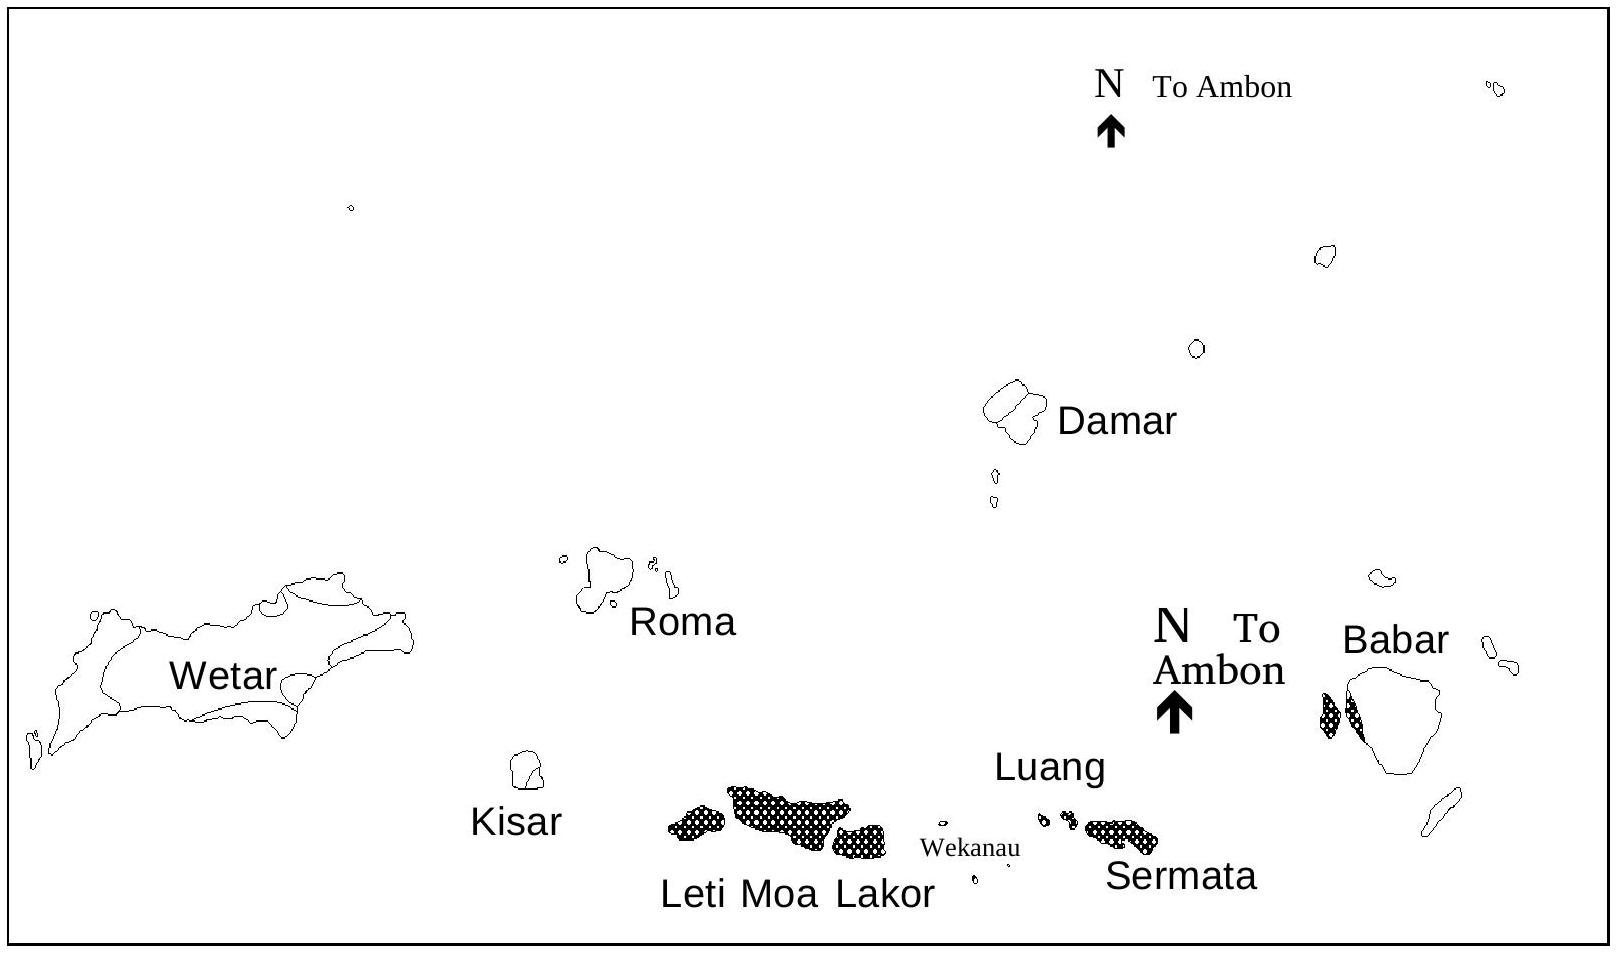
\includegraphics[width=\textwidth]{2025_09_03_818715438e96f16321bbg-012}
\end{center}
\end{figure}

The shaded area is where the various dialects of the Luang language are spoken.

\section*{2 Phonology}
\subsection*{2.1 Description of Luang phonemes}
\subsection*{2.1.1 Listing of phonemes}
The Luang dialect has a total of twenty phonemes distributed between two major classes of phonemes, consonants and vowels. \({ }^{6}\) The supra-segmental features of stress and length are important and interesting features though not phonemically distinctive in Luang. Intonation, which is phonemic, will be briefly mentioned in §2.1.5.3 below. Tables 1 and 2 below show the Luang sound system that consists of fifteen consonants and five vowels. \({ }^{7}\)

The consonantal system may be described as having three points of articulation: labial, which includes /pfmw/, apical /tdsnlry/, and dorsal /k \(\mathrm{l} \mathrm{g} \mathrm{h} /\). The phonemes under these points of articulation are further differentiated by their manner of articulation which distinguishes six stops /p t d k g 1/, three fricatives /f s h/, two nasals /m n/, a lateral /l/, a trill /r/, and two glides /w y/ (see table 1 below).

\footnotetext{\({ }^{6}\) The special characters used in this paper follow the revised (1989) International Phonetic Alphabet. [Phonetic], /phonemic/ and |morphophonemic| transcriptions use the accompanying brackets. Stress is marked as ' (a straight apostrophe).\\
7/b/ is not listed with the phoneme inventory because it occurs only in loan words.
}\begin{table}[h]
\begin{center}
\captionsetup{labelformat=empty}
\caption{Table 1. Luang consonants}
\begin{tabular}{|llll|}
\hline
 & Labial & Apical & Dorsal \\
Stop vl. & p & t & k \\
Stop vd. &  & d & g \\
Fricative & f & s & h \\
Nasal & m & n &  \\
Lateral &  & 1 &  \\
Trill &  & r &  \\
Glide & w & y &  \\
\hline
\end{tabular}
\end{center}
\end{table}

The vocalic system may also be described as having three points of articulation: front, central, and back. They include the following phonemes: front \(/ \mathrm{i} \mathrm{e} /\), central \(/ \mathrm{a} /\) and back \(/ \mathrm{u} \mathrm{o} /\). These phonemes are further distinguished by the height of the tongue (high, mid or low) when producing them (see table 2 below).

\begin{table}[h]
\begin{center}
\captionsetup{labelformat=empty}
\caption{Table 2. Luang vowels}
\begin{tabular}{|llll|}
\hline
 & Front & Central & Back \\
High & i &  & u \\
Mid & e &  & o \\
Low &  & a &  \\
\hline
\end{tabular}
\end{center}
\end{table}

Another way of looking at the distinctive features of Luang phonemes can be seen in tables 3 and 4 below.

\begin{table}[h]
\begin{center}
\captionsetup{labelformat=empty}
\caption{Table 3. Distinctive feature chart of Luang consonants}
\begin{tabular}{|l|l|l|l|l|l|l|l|l|l|}
\hline
 & p & t & d & k & g & ? & f & s & h \\
\hline
Sonorant & - & - & - & - & - & - & - & - & - \\
\hline
Continuant & - & - & - & - & - & - & + & + & + \\
\hline
Anterior & + & + & + & - & - & - & + & - & - \\
\hline
Coronal & - & + & + & + & - & - & - & + & - \\
\hline
Voice & - & - & + & - & + & - & - & - & - \\
\hline
 & m & n & 1 & \(\mathbf{r}\) & w & y &  &  &  \\
\hline
Sonorant & + & + & + & + & + & + &  &  &  \\
\hline
Anterior & + & + & + & + & + & - &  &  &  \\
\hline
Coronal & - & + & + & + & - & - &  &  &  \\
\hline
Nasal & + & + & - & - & - & - &  &  &  \\
\hline
Lateral & - & - & + & - & - & - &  &  &  \\
\hline
\end{tabular}
\end{center}
\end{table}

\begin{table}[h]
\begin{center}
\captionsetup{labelformat=empty}
\caption{Table 4. Distinctive feature chart of Luang vowels}
\begin{tabular}{|lccccc|}
\hline
 & i & e & a & o & u \\
High & + & - & - & - & + \\
Low & - & - & + & - & - \\
Back & - & - & + & + & + \\
Round & - & - & - & + & + \\
\hline
\end{tabular}
\end{center}
\end{table}

\subsection*{2.1.2 Interpretation of ambiguous segments}
\subsection*{2.1.2.1 Glides and high vowels}
Among the several ambiguous segments in Luang are the vocoids [i] and [u]. The status of these segments can be determined by looking at their distribution within the syllable. In syllable peaks these phones function as vowels and are thus interpreted \(/ \mathrm{i} /\) and \(/ \mathrm{u} /\) respectively. Note the following:

\begin{center}
\begin{tabular}{|l|l|l|}
\hline
['?ida] & /hida/ & 'one' \\
\hline
['rinə] & /hina/ & 'mother' \\
\hline
['nihi] & /nihi/ & 'tooth' \\
\hline
['?uhu] & /?uhu/ & 'breast' \\
\hline
['nurnu] & /nur-nu/ & 'his/her mouth' \\
\hline
['ru?ru] & /ru?ru/ & 'bow head' \\
\hline
['niyi] & /niyi/ & 'snake' \\
\hline
\end{tabular}
\end{center}

In the onset of syllables these segments function as consonants and are interpreted as the glides /w/ and \(/ \mathrm{y} /\). Note the following:

\begin{center}
\begin{tabular}{|l|l|l|}
\hline
[yo'Torə] & /yo@ora/ & 'wave' \\
\hline
[yav'yaurə] & /yawyawra/ & 'early morning' \\
\hline
[wa'yowə] & /wayowa/ & 'agree' \\
\hline
['wavi] & /wawi/ & 'pig' \\
\hline
['wawannu] & /wawan-nu/ & 'on top of' \\
\hline
['rayi] & /rayi/ & 'land' \\
\hline
\end{tabular}
\end{center}

In syllable codas, \([\mathrm{i}]\) and \([\mathrm{u}]\) may function as consonants or vowels depending upon the placement of stress. When they are vowels they count for stress, when they function as consonants they do not. Their interpretation must also adhere to the unambiguous syllable patterns in the language, one of these being that no vowel clusters of three can occur.

\begin{center}
\begin{tabular}{|l|l|l|}
\hline
['taili] & /tayli/ & 'weigh' \\
\hline
['3au] & /hau/ & 'wood' \\
\hline
['pwou] & /pwou/ & 'sail boat' \\
\hline
['kryou] & /kryou/ & 'k.o. basket' \\
\hline
['ravtu] & /rawtu/ & 'scratch' \\
\hline
[yav'yauræ] & /yawyawra/ & 'early morning' \\
\hline
\end{tabular}
\end{center}

\subsection*{2.1.2.2 Labialized consonants}
The labialization of consonants is a common occurence in Luang due to the morphophonemic processes that take place (see §2.3.3 below). There are also a few unambiguous environments where labialization of consonants occurs. In both the conditioned and unconditioned environments these phones are interpreted as consonant sequences /Cw/ rather than single phonemes / \(\mathrm{C}^{\mathrm{W}} /\) in order to economize phonemes. This interpretation is supported by the fact that the labialized consonants only occur syllable initially where other consonant clusters are found (see §2.2.2 below) and therefore remain consistent with acceptable syllable patterns in Luang. Labialization occurs on only labial consonants.

\begin{center}
\begin{tabular}{lll}
\(\left[' \mathrm{~m}^{\mathrm{W}} \mathrm{ai}\right]\) & \(/ \mathrm{mwai} /\) & 'you sg. come' \\
\(\left[' \mathrm{p}^{\mathrm{W}} \mathrm{ei}\right]\) & \(/ \mathrm{pwei} /\) & 'you sg. wait' \\
\(\left[\mathrm{Tamp}^{\mathrm{w}} \mathrm{a}^{\prime} \mathrm{haru}\right]\) & \(/\) Tampwaharu/ & 'we talk about' \\
\end{tabular}
\end{center}

\begin{center}
\begin{tabular}{lll}
\(\left[' \mathrm{~m}^{\mathrm{w}}\right.\) ana \(]\) & /mwana/ & 'West Luang village' \\
\(\left[' \mathrm{~m}^{\mathrm{w}}\right.\) anu \(]\) & /mwanu/ & 'male' \\
\(\left[' \mathrm{p}^{\mathrm{w}}\right.\) atə \(]\) & /pwata/ & 'female' \\
\end{tabular}
\end{center}

\subsection*{2.1.2.3 Palatalized consonants}
Like labialization, the palatalization of consonants is a common occurence in Luang due to the morphophonemic processes that take place (see §2.3.3 below). There are also a few unambiguous environments where palatalization of consonants occurs. In both the conditioned and unconditioned environments these phones are interpreted as consonant sequences /Cy/ rather than single phonemes \(/ \mathrm{C}^{\mathrm{y}} /\) in order to economize phonemes. This interpretation is supported by the fact that the palatalized consonants only occur syllable initially where other consonant clusters are found (see \(\S 2.2 .2\) below) and therefore remain consistent with the acceptable syllable patterns in Luang. Palatalization occurs on the following consonants (except ? ) /t d k sh n l r/.

\begin{center}
\begin{tabular}{|l|l|l|}
\hline
[ \(2 \mathrm{a}^{1} \mathrm{t}^{\mathrm{y}}\) ayli] & /?ai-tyayli/ & 'I weigh' \\
\hline
[ Pai \(^{\text {d }}{ }^{\text {y }}\) cllә] & /?ai-dyel-la/ & 'I stay' \({ }^{8}\) \\
\hline
[?om'k \({ }^{\text {y }}\) ohu] & /?om-kyohu/ & 'you sg. tie' \\
\hline
[?ai's \({ }^{\text {y }}\) ayni] & /?ai-syayni/ & 'I love' \\
\hline
[mn \({ }^{\text {y }}\) ayri] & /m-nyayri/ & 'you sg. wear' \\
\hline
[ ใom'l \({ }^{\text {У }}\) aใә] & /?om-lyaaa/ & 'you sg. go' \\
\hline
[ \(3 \mathrm{om}^{\prime} \mathrm{r}^{\mathrm{y}}\) anə] & /?om-ryana/ & 'you sg. pick up' \\
\hline
['nat \({ }^{\text {y }}\) ana] & /na-tyana/ & 'he/she asks' \\
\hline
['kăd \({ }^{\text {y }}\) eli] & /kdyeli/ & 'ring' \\
\hline
['k \({ }^{\text {y }}\) o? ว] & /kyora/ & 'salt' \\
\hline
['h \({ }^{\text {y }}\) aʔə] & /hyaʔa/ & 'what' \\
\hline
[1 \({ }^{\text {Ye }}\) e'2elə] & /lyeใela/ & 'k.o. shell' \\
\hline
[na'r \({ }^{\text {y }}\) ei] & /na-ryei/ & 'he/she teases' \\
\hline
\end{tabular}
\end{center}

\subsection*{2.1.2.4 Syllabic consonants}
In Luang the syllabic consonants /m n rlk/ occur. They occur in two main environments. One of these is the prefixation of verb roots (see §2.4.2 below). The other environment is the addition of affixes for derivational purposes. Since these syllabic consonants occur in predictable environments they are not considered phonemic in order to conserve phonemes. In connected speech, as opposed to isolated examples, these word initial syllabic consonants are not syllabic, but instead become a syllable coda in the preceding word.

\begin{center}
\begin{tabular}{lllll}
\([\mathrm{n}]+[\) 'nayri \(]=[\) n'nayri \(]\) & \(/\) n-nayri \(/\) & \(/\) hade nnayri/ & ['haden 'nayri] & 'she/he uses' \\
\([\mathrm{r}]+[\) 'ran \(\ni]=[\) 'rran \(\ni]\) & \(/\) r-rana/ & /ha rrana/ & ['har 'ran \(\mathfrak{}\) ] & 'she/he lifts' \\
\([\mathrm{m}]+[\) nur'nuhru \(]=[\) mnur'nuhru \(]\) & \(/\) m-nur-nuhru/ & /koka mnurnuhru/ & ['kokam nur'nuhru] & 'silky cloth' \\
\([\mathrm{k}]+[\) leha \(]=[\) kleha \(]\) & /kleha/ & /na-kleha/ & ['nak-leha] & 'she/he lacks' \\
\end{tabular}
\end{center}

\footnotetext{\({ }^{8}\) The palatal sequences /ty/ and /dy/ are often realized as the affricates [tj] and [dʒ] in fast speech.
}\subsection*{2.1.2.5 Short epenthetic schwa}
A common feature in Luang is the epenthetical schwa [ә̆] which occurs between non-homorganic consonants across syllable boundaries. However when non-homorganic consonant clusters occur syllable initial within a syllable, and if the second member of the cluster is the liquid \(/ \mathrm{l} / \mathrm{or} / \mathrm{r} /\) then no epenthesis occurs. Therefore, because its environment is predictable in that it signals a syllable break between two non-homorganic consonants, this epenthetic schwa is considered to be non-phonemic. \({ }^{9}\) The timing is also significantly shorter than a normal vocoid and it is not perceived as being distinctive by native speakers.

Examples between syllables within a morpheme:

\begin{verbatim}
['memә̆nә] /memna/ 'very'
['wuʔว̆ru] /wu?ru/ 'cooking oil'
['m\varepsilonhә̆rコ] /mehra/ 'sick'
[kală'wedə] /kalweda/ 'greeting/leave taking'
['?apә̆nu] /?apnu/ 'stomach'
['plokә̆rə] /p-lokra/ 'sharp'
\end{verbatim}

Examples between syllables within a word, (note that insertion follows stress placement):

\begin{verbatim}
['tutăgə] /tut-ga/ 'point-it'
['limăni] /lim-ni/ 'his/her hand'
['lakăni] /lak-ni/ 'his/her foot'
\end{verbatim}

Examples syllable initial with liquids /l/ and /r/:

\begin{verbatim}
['tre?a] /tre2a/ 'left'
['prai] /prai/ 'k.o.drum'
['tlinә] /tlina/ 'ear'
\end{verbatim}

\subsection*{2.1.3 Consonants}
This section provides a technical description of all Luang phonemes and their phonetic realizations. Where helpful, phonological rules are included to summarize the phonological processes described.

\subsection*{2.1.3.1 Stops}
/p/ [p] is a voiceless bilabial unaspirated plosive. It occurs word initially and medially, but as with all consonants never word finally.

\begin{verbatim}
[po'?orә] /po?ora/ 'skinny'
['poli] /poli/ 'pants'
['gә̆hә̆рә] /gehpa/ 'rotten'
['?apănu] /?apnu/ 'stomach'
\end{verbatim}

\begin{verbatim}
clustering together as they do elsewhere.
    ['ităra] /it.ra/ 'add'
    ['putăra] /put.ra/ 'deceive'
    ['tremә] /tre.ma/ 'almost'
    [na'trimә] /na.tri.ma/ 'he/she receives'
\end{verbatim}

\({ }^{9}\) An epenthetic break can also occur between the homorganic phonemes \(/ \mathrm{t} /\) and \(/ \mathrm{r} /\) where they occur morpheme\\
medially. It is this epenthetic break which signals that these phonemes occur across syllable boundaries and are not\\[0pt]
/t/ [t] is a voiceless dental unaspirated plosive. It occurs word initially and medially.

\begin{center}
\begin{tabular}{lll}
['torr] & /tora/ & 'knee' \\[0pt]
['tcrnu] & /ternu/ & 'egg' \\[0pt]
[?awa'tutu] & /?awatutu/ & 'I teach/learn' \\[0pt]
['watu] & /watu/ & 'rock' \\
\end{tabular}
\end{center}

/d/ [d] is a voiced alveolar plosive. It occurs word initially and medially

\begin{center}
\begin{tabular}{lll}
[dodo'ionə] & /dodo?ona/ 'earlier' &  \\[0pt]
[donnə] & /donna/ & 'NEG' \\[0pt]
['idə] & /ida/ & 'one' \\[0pt]
[ha'dewə] & /hadewa/ & 'enough' \\
\end{tabular}
\end{center}

/k/ [k] is a voiceless velar unaspirated plosive. It occurs word initially and medially.

\begin{center}
\begin{tabular}{lll}
['kɛrnә] & /kerna/ & 'dry' \\[0pt]
[kɛn'ku?ə] & /ken-ku?a/ & 'child' \\[0pt]
['woki] & /woki/ & 'cold' \\[0pt]
['niki] & /niki/ & 'fruit bat' \\
\end{tabular}
\end{center}

\(/ \mathrm{g} /[\mathrm{g}]\) is a voiced velar plosive and is in free variation with the voiced velar fricative [ \(\gamma\) ]. It occurs word initially and medially. \({ }^{10}\)

\begin{center}
\begin{tabular}{lll}
['gayni] \~{} ['yayni] & /gay-ni/ & 'face' \\[0pt]
[ga''2ar \(\Theta\) ] \(\sim\) [ya'2arə] & /ga2ara/ & 'root' \\[0pt]
[wo'gatə] \(\sim\) [wo'yatə] & /wo-gata/ & 'four' \\[0pt]
[2or'gahi] \(\sim\) [2or'yahi] & /or-gahi/ & 'Creator God' \\
\end{tabular}
\end{center}

/?/ [?] is a glottal stop. It occurs word initially and medially. Glottal stop is phonemic in Luang due to its contrast with other phonemes (see §2.1.3.6 below) and because native speakers recognize it as being distinctive. \({ }^{11}\)

\begin{center}
\begin{tabular}{lll}
['2aʔu] & /ใaʔu/ & 'I' \\[0pt]
['idə] & /?ida/ & 'one' \\[0pt]
['tah?i] & /tah?i/ & 'near/shallow sea' \\[0pt]
[hap'peใә] & /ha-p-peia/ 'older female' &  \\[0pt]
[wo'ใorə] & /wo?ora/ 'mountain' &  \\
\end{tabular}
\end{center}

\subsection*{2.1.3.2 Fricatives}
/f/ [f] is a voiceless labiodental fricative. It only occurs word initially. \({ }^{12}\)

\begin{center}
\begin{tabular}{lll}
['follə] & /folla/ & 'window' \\[0pt]
[fi'ayarni] & /fiayar-ni/ & 'its tree sap' \\[0pt]
[fi'દktə] & /fiekta/ & 'quick' \\[0pt]
[fi'enə] & /fiena/ & 'name of island' \\
\end{tabular}
\end{center}

\footnotetext{\({ }^{10}\) The older generation produce a voiced velar fricative [ \(\gamma\) ] rather than the voiced velar plosive.\\
\({ }^{11}\) Although glottal stop is predictable word initially preceding vowels (e.g., ['ʔidә] 'one') it is considered to be phonemic in this position as well since it undergoes morphophonemic processes (see §2.4.3 below).\\
\({ }^{12} / \mathrm{f} /\) is considered a suspect phoneme because it only occurs six times in all our data (which includes a lexicon of over 2500 words), and two of those are known loan words (see above examples marked with *). Also there is no evidence of even a phonetic [f] in the two closest related languages to Luang: Roma (Steven 1991) and Kisar (Christensen 1992). /f/ may be a phoneme in transition, but more research is needed to determine its exact status.
}\begin{center}
\begin{tabular}{lll}
[fa2'anə] & /fa'ana/ & 'abundance' \\[0pt]
['fotว̆wə] & /fotwa/ & 'picture/photo'* \\[0pt]
[fɛl'pɛnni] & /felpen-ni/ & 'pen'* \\
\end{tabular}
\end{center}

/s/ [s] is a voiceless alveolar fricative. It occurs word initially and medially but is always morpheme initial. \({ }^{13}\)

\begin{verbatim}
[sa'ponni] /sa-pon-ni/ 'it is big'
[sa'mou] /sa-mou/ 'it is good'
[?\varepsilonn'sampe] /en-sampe/ 'he/she arrived'
[na'senə] /na-sena/ 'he/she coughs'
\end{verbatim}

/h/ [h] is a voiceless glottal fricative. It occurs word initially and word medially.

\begin{verbatim}
['hadi] /hadi/ 'this'
[hon'nonә] /honnona/ 'all'
['rahu] /rahu/ 'hundred'
['2ahu] /?ahu/ `dog'
\end{verbatim}

\subsection*{2.1.3.3 Nasals}
\(/ \mathrm{m} /[\mathrm{m}]\) is a voiced bilabial nasal. It occurs word initially and medially.

\begin{verbatim}
[mu'?unә] /muʔuna/ 'you sg. eat'
['maʔә̆nu] /ma?nu/ 'bird'
['limә̆ni] /lim-ni/ 'his hand'
['amә] /.ama/ 'father'
\end{verbatim}

[ŋ] is a voiced velar nasal which fluctuates freely with [m] in the environment preceding /k/ according to speaker.

\begin{verbatim}
[?ɛmka'meni] ~ [?ɛŋka'meni] /emkameni/ 'how'
[ram'keka] ~ [raŋ'kekə] /ra-mkeka/ 'they see'
\end{verbatim}

\footnotetext{\(13 / \mathrm{s} /\) is an intriguing phoneme because by all appearances it seems to have just arrived on the scene in the last generation. Previously / \(\mathrm{h} /\) was used exclusively in Luang for PMP *s. In some of the other Luang dialects /s/ is used (e.g., in Leti, see chart below). However, according to native Luang speakers, only in the last generation has /s/ begun to be used in the Luang dialect. It appears to have come into use through the introduction of loan words and as a result of formal education in Indonesian, the national language of Indonesia. The common occurrence of intermarriage between dialects of Luang affects the use of /h/ and /s/. Some words are spoken with either /h/ or /s/ depending on the age and/or background (education) of the speaker as in the above example /saponni/. In other words (e.g., /samou/), it already appears to have become a frozen form with everyone using /s/. However, this is only a general observation and will require further study. When questioning the elders in Luang about this shift they typically respond, "yes, the real form of the word is /nahena/ 'he/she coughs', but now we say /nasena/ 'he/she coughs'."
}\begin{center}
\begin{tabular}{|l|l|l|l|l|l|}
\hline
\multicolumn{3}{|l|}{Leti /s/ - Luang /h/} & \multicolumn{3}{|l|}{PMP Form *s - Luang /h/} \\
\hline
Leti - & /memese/ 'alone' &  & PMP - & /asu/ & 'dog' \\
\hline
Luang - & /memeha/'alone' &  & Luang - & /ahu/ & 'dog' \\
\hline
Leti - & /syaa/ & 'what?' & PMP - & *taSik & 'sea' \\
\hline
Luang - & /hyaʔa/ & 'what?' & Luang - & /tahʔi/ & 'sea' \\
\hline
Leti - & /nusa/ & 'island' & PMP - & *susu & 'breast' \\
\hline
Luang - & /noha/ & 'island' & Luang - & /uhu/ & 'breast' \\
\hline
\end{tabular}
\end{center}

/n/ [n] is a voiced alveolar nasal. It occurs word initially and medially.

\begin{center}
\begin{tabular}{lll}
['norə] & /nora/ & 'coconut' \\[0pt]
['namăni] & /nam-ni/ & 'his tongue' \\[0pt]
['matni] & /mat-ni/ & 'his eye' \\[0pt]
['tcrnu] & /tcrnu/ & 'egg' \\
\end{tabular}
\end{center}

[ n ] is a voiced velar nasal which fluctuates freely with [ n ] in the environment preceding / \(\mathrm{k} /\) according to speaker.

\begin{verbatim}
[k\varepsilonn'ku?a] ~ [kɛŋ'ku?ə] /ken-ku?a/ `child’
[man'keʔว] ~ [maŋ'keʔə] /man-keʔa/ 'man'
\end{verbatim}

With some speakers there is neutralization of contrast between \(/ \mathrm{m} /\) and \(/ \mathrm{n} /\) preceding \(/ \mathrm{k} /\).

\begin{verbatim}
[nam'kekə] ~ [naŋ'kekə] /nam-keka/ `she/he sees`
\end{verbatim}

\subsection*{2.1.3.4 Liquids}
/l/ [l] is a voiced alveolar lateral. It occurs word initially and medially.

\begin{verbatim}
['lerə] /lera/ `sun/day'
['lorә] /lora/ 'ocean'
['wolla] /wolla/ 'moon'
['wali] /wali/ 'again'
\end{verbatim}

\(/ \mathrm{r} /[\mathrm{r}]\) is a voiced alveolar trill. It occurs word initially and medially. \({ }^{14}\)

\begin{verbatim}
['ruri] /ruri/ 'thorn'
['reri] /reri/ 'very'
['norә] /nora/ 'coconut'
['kɛrnә] /kerna/ `dry'
\end{verbatim}

\subsection*{2.1.3.5 Glides}
\(/ \mathrm{w} /[\mathrm{w}]\) is a voiced bilabial glide. It is produced with less lip rounding and more friction than the English [w]. It occurs word initially and medially.

\begin{verbatim}
[wa'?anә] /wa2ana/ 'again'
[wo'?awә] /wo?awa/ 'eight'
['plahว̆wə] /plahwa/ 'long'
['wawanu] /wawan-nu/ 'on top of'
\end{verbatim}

[v] is a voiced labiodental approximate. This phone occurs in two environments: following a vowel and preceding a consonant or preceding liquids word initially.

\begin{verbatim}
['wevә̆n\mathfrak{] /wewna/ 'k.o. grass'}
[2auri'ehə] //awrieha/ 'rice'
['vlari] /wlari/ 'run'
['vra?u] /wra2u/ 'plate'
\end{verbatim}

\footnotetext{\({ }^{14}\) Sometimes in fast speech /r/ will change its manner of articulation and be realized as a flap [rㅏ] intervocalically. [ruri].\~{} [ruři] 'thorn' [rarə].\~{}.[rařə] 'blood'
}
[v] is a voiced labiodental fricative. This phone occurs intervocalically between two high vowels. In between a non-high vowel and a high vowel, this phone fluctuates freely with a voiced bilabial fricative [ß].

\begin{verbatim}
['hivi] /hiwi/ 'chicken'
['wuvu] /wuwu 'clan'
['?avu] ~ ['?aßu] /?awu/ 'dust'
['wavi] ~ ['waßi] /wawi/ 'pig'
\end{verbatim}

The rule for /w/ is:/w/ - \(\rightarrow\) [v] / V\_C, \#\_/l/, /r/

\begin{verbatim}
[v] / V + High_V + High
[v] ~ [ß] / V_V + High
[w] / \# __, C_V, V_V
\end{verbatim}

/y/ [y] is a voiced palatal glide. It occurs word initially and medially.

\begin{center}
\begin{tabular}{lll}
['yomə] & /yoma/ & 'because' \\[0pt]
['yav'yaurə] & /yawyawra/ & 'early morning' \\[0pt]
[?ɛnkah'yoyə] / Ren-kahyoya/ & 'he/she bounces up and down' &  \\
\end{tabular}
\end{center}

\subsection*{2.1.3.6 Consonant contrasts}
\begin{verbatim}
p/m/w
    ['polu] /polu/ 'call'
    ['molu] /molu/ 'lost'
    ['woru] /woru/ 'two'
    ['2upә] /upa/ 'mouse'
    ['2amә] /ama/ 'father'
    ['wawә] /wawa/ 'mouth'
    [pepăna] /pepna/ 'encircle'
    [memăna] /memna/ 'very'
    [wewว̆nə] /wewna/ 'grass'
p/f/w
    ['polә] /pola/ 'return'
    ['follә] /folla/ 'window'
    ['wollә] /wolla/ 'moon'
t/d/r
    ['tonә] /tona/ `soak'
    ['donnә] /donna/ 'NEG'
    ['romә] /roma/ 'house'
    ['?ita] /?ita/ 'we (incl.)'
    ['?ida] /?ida/ 'one'
    ['iiræ] /?ira/ 'they'
t/d/n/l
    ['turu] /turu/ 'come down'
    ['durmә] /durma/ 'divide'
    ['nurnu] /nur-nu/ 'mouth'
    ['lirni] /lir-ni/ 'his voice'
\end{verbatim}

\begin{verbatim}
    ['torə] /tora/ 'knee'
    ['dohә] /doha/ 'hair piece'
    ['nohә] /noha/ `island'
    ['lorə] /lora/ `sun'
    ['?ita] /?ita/ `we (incl.)'
    ['2idə] /?ida/ 'one'
    ['ina] /?ina/ 'mother'
    ['iili] /iili/ 'stone'
k/g/?/h
    ['karmә] /karma/ 'k.o. tree'
    ['garni] /gar-ni/ 'his younger sibling'
    ['?arnә] /?arna/ 'breathe'
    ['harni] /har-ni/ 'part of coconut tree'
    ['kɛrnә] /kerna/ `dry'
    ['gerә] /gera/ 'water'
    ['{crlə] /?erla/ 'there are'
    ['heræ] /hera/ 'port'
    ['nokә] /noka/ 'then'
    [sa'mogә] /samoga/ 'good'
    ['po?ә] /po?a/ 'areca nut'
    ['nohә] /noha/ 'island'
    [na'kowə] /na-kowa/ 'lay prone/face up'
    [wo'gatə] /wo-gata/ 'four'
    [wo'?awә] /wo-{awa/ 'eight'
    [na'hawə] /na-hawa/ 'he/she mates'
?/ø
    ['?a?u] /?a?u/ 'I'
    ['?au] /?au/ `wood'
    ['pah?ә] /pah2a/ `break'
    ['mahә] /maha/ 'gold'
    ['ta2wә] /ta2wa/ 'knife'
    ['tawə] /tawa/ 'k.o. seaweed'
s/h
    [sa'ponni] /sa-pon-ni/ 'very big'
    [hap'pe?ә] /ha-p-pe?a/ 'older female'
    [na'sen\partial] /na-sena/ 'he/she coughs'
    [na'hepru] /na-hepru/ 'he/she laughs'
m/n
    ['moræ] /mora/ `you sg. and'
    ['norə] /nora/ 'coconut'
\end{verbatim}

\begin{verbatim}
    ['romә] /roma/ 'house'
    ['tonә] /tona/ `soak'
l/r
\end{verbatim}

\begin{verbatim}
['lerə] /lera/ 'sun'
['rerә] /rera/ 'post/pole'
['ralə] /rala/ 'they give'
['rarə] /rara/ 'blood'
\end{verbatim}

\(\mathrm{y} / \mathrm{g} / \mathrm{l} / \mathrm{m} / \mathrm{h}\)

\begin{verbatim}
['yerә] /yera/ 'sister-in-law'
['gerә] /gera/ 'water'
['lerə] /lera/ 'sun'
['merә] /mera/ 'but'
['heræ] /hera/ 'port'
\end{verbatim}

\subsection*{2.1.4 Vowels}
\subsection*{2.1.4.1 Description}
/i/ [i] is a high close front unrounded vocoid. It occurs word medially and finally. It occurs in stressed, and post-stressed syllables. It can also occur in pre-stressed syllables when there are more than two syllables.

\begin{center}
\begin{tabular}{lll}
['Rinə] & /?ina/ & 'mother' \\[0pt]
['ində] & /?ida/ & 'one' \\[0pt]
[wo'limə] & /wo-lima/ & 'five' \\[0pt]
['pipi] & /pipi/ & 'goat' \\[0pt]
['woki] & /woki/ & 'cold' \\[0pt]
['garni] & /gar-ni/ & 'his younger sibling' \\[0pt]
[i'hini] & /ihi-ni/ & 'its-insides' \\
\end{tabular}
\end{center}

/e/ [e] is a mid close front unrounded vocoid. It generally occurs word finally although it can sometimes occur word medially in a CV syllable pattern depending on the speaker. It occurs in both stressed and post-stressed syllables.

\begin{center}
\begin{tabular}{lll}
[wo'telu] & /wo-telu/ & 'three' \\[0pt]
['re] & /re/ & 'those' \\[0pt]
['mere] & /mere/ & 'but' \\[0pt]
['hade] & /hade/ & 'that' \\[0pt]
['hare] & /hare/ & 'they' \\
\end{tabular}
\end{center}

\([\varepsilon]\) is a mid open front unrounded vocoid. It occurs word medially in closed syllables. It occurs in stressed and pre-stressed syllables.

\begin{center}
\begin{tabular}{lll}
[?ɛcm'kade] & /?emkade/ & 'like that' \\[0pt]
['İsnu] & /?enu/ & 'sea turtle' \\[0pt]
['tɛrnu] & /ternu/ & 'egg' \\[0pt]
['mɛhә̆rコ] & /mehra/ & 'sick' \\
\end{tabular}
\end{center}

The rule for /e/ is: /e/ - \(\rightarrow\)\\[0pt]
[ɛ] / \# ?\_\_, \(\qquad\) C\$\\[0pt]
[e] / Elsewhere\\[0pt]
/a/ [a] is a low open central unrounded vocoid. It occurs word medially. It occurs in stressed syllables. It also occurs in pre-stressed syllables when the word has more than two syllables.

\begin{center}
\begin{tabular}{lll}
['2ahu] & /?ahu/ & 'dog' \\[0pt]
['2aßu] & /?awu/ & 'dust' \\[0pt]
['watu] & /watu/ & 'rock' \\[0pt]
['manə] & /mana/ & 'also' \\[0pt]
[aßri'ehə] & /awrieha/ & 'uncooked rice' \\
\end{tabular}
\end{center}

[ə] is a mid open central unrounded vocoid. It occurs word finally. It occurs in stressed and poststressed syllables.

\begin{center}
\begin{tabular}{lll}
[pi'parə] & /pipara/ & 'cook' \\[0pt]
['gerə] & /gera/ & 'water' \\[0pt]
['pə] & /pa/ & 'to' \\
\end{tabular}
\end{center}

The rule for /a/ is: /a/ - \(\rightarrow\) [ \(\mathfrak{a}\) ] / \_\_\#\\[0pt]
[a] / \(\qquad\)\\[0pt]
/o/ [o] is a mid close back rounded vocoid. It occurs word medially. \({ }^{15}\) It occurs in stressed syllables and in pre-stressed syllables if there are more than two syllables in the word.

\begin{center}
\begin{tabular}{lll}
['2orә] & /?ora/ & 'k.o. bamboo' \\[0pt]
[?o'keใə] & /?okeʔa/ & 'a little' \\[0pt]
['wollə] & /wolla/ & 'moon' \\[0pt]
['woki] & /woki/ & 'cold' \\[0pt]
['kohu] & /kohu/ & 'tie' \\
\end{tabular}
\end{center}

\(/ \mathrm{u} /[\mathrm{u}]\) is a high close back rounded vocoid. It occurs word medially and finally. It occurs in stressed and post-stressed syllables. It can also occur in pre-stressed syllables when there are more than two syllables in the word.

\begin{center}
\begin{tabular}{lll}
['2uhu] & /?uhu/ & 'breast' \\[0pt]
['2upә] & /?upa/ & 'grandchild/parent' \\[0pt]
['tutu] & /tutu/ & 'point' \\
 &  &  \\[0pt]
['ruri] & /ruri/ & 'thorn' \\[0pt]
['petu] & /petu/ & 'k.o. bamboo' \\[0pt]
['2ahu] & /hahu/ & 'dog' \\[0pt]
[nu'nuhru] & /nunuhru/ & 'runny nose' \\
\end{tabular}
\end{center}

\subsection*{2.1.4.2 Contrasts}
\section*{a/e/i/o/u}
\begin{center}
\begin{tabular}{lll}
['2anni] & /?anni/ & 'wind' \\[0pt]
['2snni] & /?en-ni/ & 'his findings/catch' \\[0pt]
['2inni] & /?in-ni/ & 'his mother' \\[0pt]
['2onni] & /?on-ni/ & 'tree' \\[0pt]
['?unnu] & /?un-nu/ & 'cluster' \\
\end{tabular}
\end{center}

\footnotetext{¹5/o/ only occurs word finally when it functions as a phrase level enclitic indicating emphasis (see §2.1.5.1 below).\\[0pt]
[kal'wedə] \(\rightarrow\) [kalwe'do] 'emphasized greeting'\\[0pt]
['handelə] \(\rightarrow\) [hande'lo] 'way over there'
}\begin{verbatim}
a/e
    ['2ati] /?ati/ 'liver'
    ['2cti] /?eti/ 'very'
    [mar'marә] /mar-mara/ 'yellow'
    [m\varepsilonr'merə] /mer-mera/ 'red'
    ['?ida] /?ida/ 'one'
    ['hade] /hade/ 'that'
a/u
    ['?ahu] /?ahu/ 'dog'
    ['?uhu] /?uhu/ 'breast'
    ['rarni] /rar-ni/ 'his blood'
    ['rurni] /rur-ni/ 'his bone'
    ['nohә] /noha/ 'island'
    ['nuhu] /nuhu/ 'he/she nurses'
u/o
    ['?utu] /?utu/ 'louse'
    ['lotnә] /?otna/ 'rain'
    ['nuhu] /nuhu/ 'he/she nurses'
    ['nohә] /noha/ 'island'
i/e
    ['?irnu] /?irnu/ 'nose'
    ['?\varepsilonrnu] /?ernu/ 'go down'
    ['nihә] /niha/ 'tooth'
    ['n\varepsilonhu] /nehu/ 'jump'
    ['hadi] /hadi/ 'this'
    ['hade] /hade/ 'that'
e/o
['?e?a] /?e?a/ 'he/she'
['?o2ә] /.ho?a/ 'you sg.'
['leræ] /lera/ 'sun'
['lorə] /lora/ 'ocean'
\end{verbatim}

\subsection*{2.1.5 Supra-segmental features}
\subsection*{2.1.5.1 Stress}
In the phonological word, stress (indicated in examples by ['] preceding the stressed syllable) is manifested by increased intensity and rising pitch on the stressed syllable. Stress falls on the penultimate syllable of bisyllabic roots, and remains on the root in monosyllabic roots. Stress does not move to the\\
new penultimate syllable when affixes are added as is the case in Indonesian. Therefore, because stress is predictable it is considered to be non-phonemic in Luang.\\[0pt]
[na'pɛtnə] /na-petna/ 'he/she is fat'\\[0pt]
['pɛtannidi] /petan-ni-di/'his very fatness'\\[0pt]
['2ulti] /?ulti/ 'skin'\\[0pt]
['?ulatni] /?ulat-ni/ 'his skin'\\[0pt]
A factor that can affect the penultimate stress rule is special emphasis on the phrase level which can override word stress. (This emphasis is indicated in examples by ["] preceding the stressed syllable.) This occurs when the final vowels of the final words in the phonological phrase are deleted and the emphatic enclitics [-o] and [-e] are attached in their place. When this happens, the stress on the penultimate syllable of that word is overridden by phonological phrase stress which occurs on the final syllable of the phrase.\\[0pt]
[?ai'dyɛllə 'handelə] 'I came from over there' (normal stress)\\[0pt]
[?ai'dyɛllə hande"lo] 'I came from way over there' (emphatic)\\[0pt]
[?it'laʔawə] 'We are going' (normal)\\[0pt]
[?itlaʔa"we] 'Here we go!' (emphatic)\\
Another factor that can affect word stress is when separate grammatical words occur as one phonetic rhythm segment which can occur as the result of morphophonemic processes (see §2.4 below). When this occurs the stress on the penultimate syllable of the root becomes secondary to the phrase stress on the penultimate syllable of the rhythm segment, if the adjoining word is bisyllabic.

\[
\begin{array}{ll}
\text { [niʔə] 'make' + ['yatə̆ru] 'trap' = [niʔ'yatə̆ru] } & \text { 'make a trap' } \\
\text { ['au'rohə] 'I bathe' + ['2aʔu] 'I' = ['auro'haʔu] } & \text { 'I bathe myself' } \\
\text { ['nuri] 'pour' + ['doyni] 'ASP' = [nur'dyoyni] } & \text { 'pour it all out' }
\end{array}
\]

\subsection*{2.1.5.2 Length}
The Luang language contains phonetically long consonants and vowels. This feature of length, however, is not phonemic. The long consonants are interpreted to be a sequence of two identical phonemes or two different contiguous phonemes that assimilate. They are considered to be sequences rather than units because this interpretation economizes phonemes and still corresponds to acceptable syllable patterns. Not only do these segments occur across syllable boundaries, but most occur either as the result of morphophonemic processes or the result of non-morphophonemic historical processes e.g., /wolla/ 'moon'. These geminate segments are produced with a noticeable delay in their release. They occur both word initially and medially.

\begin{center}
\begin{tabular}{|l|l|l|l|}
\hline
[hap'peใә] & /ha-p-peใa/ &  & 'older female' \\
\hline
[2it'tallə] & /2it-talla/ &  & 'we travel together' \\
\hline
[kok'koi] & /kok-koi/ &  & 'riddle' \\
\hline
[ṃ'mwahə] & /m-mwaha/ &  & 'you sg. are tired' \\
\hline
[ņ'nayri] & /n-nayri/ &  & 'he/she wears' \\
\hline
[̣ller'nanə] & /l-lernana/ & |n-lernana| & 'he/she gets' \({ }^{16}\) \\
\hline
[ŗ'rana] & /r-rana/ &  & 'they pick up' \\
\hline
\end{tabular}
\end{center}

\footnotetext{\({ }^{16}\) See footnote 33.
}Morpheme medially, long consonants occur as a result of several different morphophonemic processes (see §2.4.2 below).

\begin{center}
\begin{tabular}{llll}
['donnə] & /donna/ &  & 'NEG' \\[0pt]
['wennə] & /wenna/ & |wenan| & 'kill' \\[0pt]
['wollə] & /wolla/ & |wolan| & 'moon' \\[0pt]
['tullə] & /tulla/ & |tulna| & 'help' \\
\end{tabular}
\end{center}

\subsection*{2.1.5.3 Intonation}
A comprehensive analysis of all the intonation patterns in Luang is beyond the scope of this paper. We will, however, mention a few of the more common features. Normally on declarative statements the peak of the intonation contour coincides with the phrase final word stress. Therefore the statement will begin at mid-pitch and continue level over all the words until the syllable before the penultimate (root) syllable of the final word in the statement \({ }^{17}\). At this point the contour falls and then sharply rises on the penultimate (root) syllable to a higher pitch where the stress occurs on the peak syllable of the statement. Then it lowers over the last syllable of the statement. This pattern may be written as 2-1-3-1 (mid-low-high-low).

\begin{verbatim}
22a?g edonna 1u3wen1na// 'I am not angry.'
22a?anu 2sukni 1en3kak1ru// 'My child likes to cry.'
22oha 2etla 2kade1ra 3wa2wan1nu// 'The cat is on the chair'18
\end{verbatim}

Exceptions to this 2-1-3-1 contour occur when the statement is emphasized such as when the emphatic enclitics [-e] and [-o] are used. In these cases the pitch is low on the penultimate syllable and then sharply rises on the ultimate syllable of the phrase. This pattern may be written as \(2-1-3 .{ }^{19}\) These affect the phonological word stress on the final word in the phrase. The stress on the penultimate syllable can no longer be heard because of the phrase level stress on the ultimate syllable as a result of the intonational contour.

\begin{center}
\begin{tabular}{ll}
\begin{tabular}{l}
2ใadonna u2wenna 2ne1ka 3ne// \\
2ใaydyella 2han1de3lo// \\
2ใitla21a4we// \\
\end{tabular} & 'I am really not angry!' \\
 & 'I came from way over there!' \\
 & 'Here we go!' \\
\end{tabular}
\end{center}

Questions follow a similar pattern as statements only the pitch is a bit higher and the decline on the ultimate syllable is more noticeable. This sharp decline in pitch often results in the devoicing of the ultimate syllable.

\begin{center}
\begin{tabular}{ll}
22omdyel1la 4me1ni// & 'Where are you sg. going?' \\
2ใomlya 2mwo?1lu 4hya1a// & 'What are going to sell?' \\
2mu?una 1?o4lek1wa// & 'Did you sg. eat yet?' \\
\end{tabular}
\end{center}

The exception to this rule is where special question tags are used to perform various functions. As with the exceptions for statements given above, the intonation has the effect of moving the normal word stress as it places the higher pitch and rising intensity on the ultimate syllable.

\begin{center}
\begin{tabular}{ll}
22omlya2a 22Apnu 1no4ka// & 'You sg. went to Ambon and then?' \\
2ใedonna 2nnayri 2ray1ni 4pa// & '(how come) She does not have any clothes on?' \\
2wolanni 2woru 22o1lek4wo// & 'She is two months (old), right?' \\
\end{tabular}
\end{center}

\footnotetext{\({ }^{17}\) This statement may be just one sentence, or a thought that encompasses a number of sentences.\\
18/wawannu/ is derived from the bisyllabic root/wawna/. In these cases where a suffix is attached, the pitch rises with the word stress and then falls evenly over the final two syllables.\\
\({ }^{19}\) The peak pitch may reach level 4 or 5 depending how expressive or animated the speaker is.
}Discourse genre is also marked by speed and cadence. In a storytelling situation as the speaker gets to an important or exciting part of the story he or she will start talking faster, higher, and with more intensity. Instead of occurring separately, grammatical words bind together to form single rhythm units. This is explained in greater detail in §2.4below.

Different genres also take on different intonational patterns. For example, procedural texts tend to have a "sing songy" up and down type rhythm (i.e., first we do this, then we do this, then we do this, etc.). Hortatory genre includes long pauses between phrases. These phrases usually start off with a rapid rhythm with high intensity and pitch which gradually slows down so that by the end of the sentence the speaker becomes soft spoken.

\subsection*{2.2 Syllables and phoneme distribution}
\subsection*{2.2.1 Syllables patterns}
There are eight syllable patterns which occur in Luang. The phonological word is composed of different combinations of the following: V, VC, CV, CVC, CCV, CCVC, CCCV and CCCVC. \({ }^{20}\) The syllable pattern CV occurs in every position of the word while VC, CVC, CCV and CCVC occur word initially and medially. V occurs only word medially and finally. CCCV and CCCVC only occur word initially. \({ }^{21}\)

\begin{table}[h]
\begin{center}
\captionsetup{labelformat=empty}
\caption{Table 5. Luang syllable patterns}
\begin{tabular}{|l|l|l|l|l|l|l|}
\hline
 & \multicolumn{2}{|l|}{Initial} & \multicolumn{2}{|l|}{Medial} & \multicolumn{2}{|l|}{Final} \\
\hline
V & - - - - - &  & 2a.ti.a.ru & 'except' & pwo.u & 'sailboat' \\
\hline
VC & ot.na & 'rain' & ri.al.ma & 'inside' & ----- &  \\
\hline
CV & ru.ri & 'thorn' & mer.me.ra & 'red' & ni.ki & 'bat' \\
\hline
CVC & ker.na & 'dry' & mot.mot.ni & 'green' & ----- &  \\
\hline
CCV & pre.yi & 'sleepy' & na.plo.la & 'it is true' & ---- &  \\
\hline
CCVC & tlin.ni & 'his ear' & na.plok.ra & 'it is sharp' & ----- &  \\
\hline
CCCV & hnya.ri & 'door' & ----- &  & ----- &  \\
\hline
CCCVC & Tnyam.ni & 'grave' & ----- &  & ----- &  \\
\hline
\end{tabular}
\end{center}
\end{table}

\subsection*{2.2.2 Consonant clusters}
\subsection*{2.2.2.1 Distribution within syllables}
There are eight unambiguous consonant clusters that occur within the syllable patterns CCV and CCVC: /pl/, /pr/, /tl/, /tr/, /kl/, /kr/, /wl/ and /wr/. As with all the other consonant clusters within a syllable, these occur only in the onset position.

\begin{center}
\begin{tabular}{lll}
['pley.ni] & /pley.ni/ & 'before' \\[0pt]
['pra.i] & /pra.i/ & 'k.o. drum' \\[0pt]
['tli.wu] & /tli.wu/ & 'calm' \\[0pt]
[tre'2eni] & /tre.eni/ & '(number of) sequences' \\[0pt]
['klokә̆.rə] & /klok.ra/ & 'one who takes an oath' \\
\end{tabular}
\end{center}

\footnotetext{\({ }^{20}\) Periods are used in the examples below to represent syllable breaks.\\
\({ }^{21}\) The syllable patterns in which three consonants occur simultaneously, such as CCCV and CCCVC do not occur within morphemes. They occur only across morpheme boundaries as a result of morphophonemic processes. The infixation of /ny/ which derives a noun from a verb is one example of this, e.g., /hari/ 'open' becomes /hnyari/ 'door'.
}\begin{center}
\begin{tabular}{lll}
['kri.tə] & /kri.ta/ & 'octopus' \\[0pt]
['vlari] & /wla.ri/ & 'run' \\[0pt]
['vraʔu] & /wra.2u/ & 'plate' \\
\end{tabular}
\end{center}

All of the other syllable onset clusters listed in table 6 occur as a result of morphophonemic processes or between morpheme boundaries. However, a number of these also occur within a morpheme. In the following table, the row shows the first consonant and the column shows the second consonant in the cluster.

\begin{table}[h]
\begin{center}
\captionsetup{labelformat=empty}
\caption{Table 6. Syllable onset clusters}
\begin{tabular}{|l|l|l|l|l|l|l|l|l|l|l|l|l|l|l|l|}
\hline
 & p & t & d & k & g & ? & f & s & h & m & n & 1 & \(\mathbf{r}\) & w & y \\
\hline
p &  &  &  &  &  &  &  &  &  &  & pn & pl & pr & pw &  \\
\hline
t &  &  &  &  & tg &  &  &  &  &  & tn & tl & tr &  & ty \\
\hline
d &  &  &  &  &  &  &  &  &  &  &  &  &  &  & dy \\
\hline
k &  &  &  &  &  &  &  &  &  &  & kn & kl & kr &  & ky \\
\hline
g &  &  &  &  &  &  &  &  &  &  &  &  &  &  &  \\
\hline
? &  &  &  &  &  &  &  &  &  &  &  &  &  &  &  \\
\hline
f &  &  &  &  &  &  &  &  &  &  &  &  &  &  &  \\
\hline
s &  &  &  &  &  &  &  &  &  &  & sn &  &  &  & sy \\
\hline
h &  &  &  &  & hg &  &  &  &  & hm & hn & hl & hr &  & hy \\
\hline
m &  &  &  &  &  &  &  &  &  &  & mn &  &  & mw &  \\
\hline
n &  &  &  &  &  &  &  &  &  &  & nn &  &  &  & ny \\
\hline
1 &  &  &  &  & \(\lg\) &  &  &  &  &  &  &  &  &  & ly \\
\hline
r &  &  &  &  &  &  &  &  &  &  &  &  &  &  & ry \\
\hline
w &  &  &  &  &  &  &  &  &  &  & wn & wl & wr &  &  \\
\hline
y &  &  &  &  &  &  &  &  &  &  &  &  &  &  &  \\
\hline
\end{tabular}
\end{center}
\end{table}

From table 6 we can see that syllable onset clusters are quite limited. The absence of certain clusters (e.g., \(/ \mathrm{ml} /\) and \(/ \mathrm{mr} /\) ) are because morphophonemic processes occur when they come together (see §2.4.1 below).

\subsection*{2.2.2.2 Distribution between syllables}
The following table lists the consonant clusters that occur across syllable boundaries.

\begin{table}[h]
\begin{center}
\captionsetup{labelformat=empty}
\caption{Table 7. Consonant clusters across syllable boundaries}
\begin{tabular}{|l|l|l|l|l|l|l|l|l|l|l|l|l|l|l|l|}
\hline
 & p & t & d & k & g & ? & f & s & h & m & \(\mathbf{n}\) & 1 & \(\mathbf{r}\) & w & y \\
\hline
p & pp &  &  &  &  &  &  &  &  & pm & pn & pl & pr & pw &  \\
\hline
t & tp & tt & td & tk & tg &  &  & ts &  & tm & tn & tl & tr & tw &  \\
\hline
d &  &  & dd &  & dg &  &  &  &  & dm & dn & dl &  & dw &  \\
\hline
k & kp & kt & kd & kk &  &  &  &  & kh & km & kn & kl & kr & kw &  \\
\hline
g &  &  &  &  &  &  &  &  &  &  &  &  &  &  &  \\
\hline
\(\mathbf{2}\) & 2p & 2t & 2d & 2k &  &  &  &  & ?h & 2m & 2n & 21 & 2r & 2w &  \\
\hline
f &  &  &  &  &  &  &  &  &  &  &  &  &  &  &  \\
\hline
s &  & st &  & sk & \multirow{3}{*}{hg} &  &  &  &  &  &  &  & sr &  &  \\
\hline
h & hp &  &  & hk &  & h? &  &  &  & hm & hn & hl & hr & hw &  \\
\hline
m & mp & mt & md & mk &  &  &  &  & mh & mm & mn & ml & mr &  &  \\
\hline
n & np & nt & nd & nk &  &  &  &  & nh & nm & nn &  & nr & nw &  \\
\hline
1 & lp & lt & ld & lk & \(\lg\) &  &  &  & lh & lm &  & 11 & lr & lw &  \\
\hline
r & rp & rt & rd & rk & rg &  &  &  & rh & rm & rn & rl & rr & rw &  \\
\hline
w & wp & wt & wd & wk &  &  &  &  &  &  &  & wl & wr &  &  \\
\hline
y &  & yt &  &  &  &  &  & ys &  & ym & yn & yl &  &  &  \\
\hline
\end{tabular}
\end{center}
\end{table}

There are several features which stand out in table 7 above. Note the absence of /f/ clustering with any other consonant. The limited distribution of /s/ can also be noted from the chart. It is interesting to note that /g/ never occurs in a consonant cluster initially, /y/ never occurs initially before other consonants between syllables, and /?/ only follows / \(\mathrm{h} /\) in the CC final position yet most everywhere initially.

There are also several "holes" that appear in table 7. Some holes are the result of phonemes such as /d/ which occur less frequently word medially. Other "holes" are valid because when those consonants cluster morphophonemic processes occur that eliminate these sequences (e.g., /nl/, /ln/, /mw/ and /wm/; see §2.4.2 below).

\subsection*{2.2.2.3 Consonant restrictions}
The consonant clusters allowable within a morpheme are more restricted than across morphemes as seen below. The consonant clusters within a morpheme which occur morpheme initial are even more restricted. They are bolded in the chart below. \({ }^{22}\)

\begin{table}[h]
\begin{center}
\captionsetup{labelformat=empty}
\caption{Table 8. Allowable consonant clusters within a morpheme}
\begin{tabular}{|l|l|l|l|l|l|l|l|l|l|l|l|l|l|l|l|}
\hline
 & p & t & d & k & g & 2 & f & s & h & m & n & 1 & r & w & y \\
\hline
p &  & pt &  &  &  &  &  &  &  &  & pn & pl & pr & pw &  \\
\hline
t &  &  &  &  &  &  &  &  &  & tm & tn & tl & tr & tw &  \\
\hline
d &  &  &  & dk &  &  &  &  &  &  & dn & dl &  & dw &  \\
\hline
k & kp & kt & kd &  &  &  &  &  &  & km & kn & kl & kr & kw &  \\
\hline
g &  &  &  &  &  &  &  &  &  &  &  &  &  &  &  \\
\hline
\(\mathbf{2}\) & 2p & 2t &  &  &  &  &  &  &  &  & 2n & 21 & 2r & 2w &  \\
\hline
f &  &  &  &  &  &  &  &  &  &  &  &  &  &  &  \\
\hline
s &  &  &  & sk &  &  &  &  &  &  &  &  &  &  &  \\
\hline
h & hp & ht &  & hk & hg & h? &  &  &  & hm & hn & hl & hr & hw &  \\
\hline
m & mp & mt &  & mk &  &  &  &  &  &  & mn & ml & mr & mw &  \\
\hline
n &  & nt & nd &  &  &  &  &  &  &  & nn &  &  &  &  \\
\hline
1 &  & lt &  &  &  &  &  &  &  & lm &  & 11 &  & lw &  \\
\hline
r &  & rt &  & rk &  &  &  &  &  & rm & rn &  &  &  &  \\
\hline
w &  & wt &  &  &  &  &  &  &  &  & wn & wl & wr &  &  \\
\hline
y &  &  &  &  &  &  &  &  &  &  & yn &  & yr &  &  \\
\hline
\end{tabular}
\end{center}
\end{table}

\subsection*{2.2.3 Vowel clusters}
All five vowels occur word initially, medially and finally. In fact, all words in Luang must end in a vowel. However, word roots never end in /o/ and verb roots never end in /o/ or /e/. \({ }^{23}\) /o/ only occurs word finally when it operates as phrase level emphatic enclitics (see §2.1.5.3 above).

\footnotetext{\({ }^{22}\) It is interesting to note that the unusual clusters such as / \(\mathrm{kp}, \mathrm{lm}, \mathrm{mn}, \mathrm{hl}, \mathrm{hg}, \mathrm{kp}, \mathrm{wt}, \mathrm{tg}, \mathrm{lg} /\) are quite limited and found almost exclusively in ritual language and in ritual names.\\[0pt]
[tgarə] /tgara/ 'ancestor'\\[0pt]
[hgerә] /hgera/ 'type of taboo/curse'\\[0pt]
[lgonə] /lgona/ 'the term Luang people call their land and language'\\
\({ }^{23}\) Although the younger generation uses /a/ word final, the older generation tend to use /e/. It may be that the \(\mathrm{a} / \mathrm{e}\) alternation used to occur only on certain words or classes of words with some meaning, but in this present generation a rule is spreading through the lexicon changing all final \(/ \mathrm{e} /\) to \(/ \mathrm{a} /\).
}\begin{table}[h]
\begin{center}
\captionsetup{labelformat=empty}
\caption{Table 9. Vowel clusters}
\begin{tabular}{|llllll|}
\hline
i & i & e & a & o & u \\
e & ei & ie & ia & io & iu \\
a & ai &  & ea &  & eu \\
o & oi &  & oa &  & au \\
u & ui & ue & ua & uo & ou \\
\hline
\end{tabular}
\end{center}
\end{table}

Table 9 shows the vowel sequences that occur in Luang across syllable boundaries. Sequences of three vowels never occur.

\subsection*{2.3 Morphophonemics}
There are many morphophonemic processes that occur in Luang. The most processes occur in two main environments, both in terms of frequency as well as type of morphophonemic process. The first environment is morpheme initial between pronominal prefixes and verb roots. The second environment is morpheme or word final position (even across word boundaries) when words phonologically join to become one rhythm segment. This includes words and their suffixes, enclitics, modifiers or even separate words that follow. These two environments are further explained below with various examples of the morphophonemic processes and the order in which they occur.

A couple other minor environments which will be discussed are the nominalizing infix /ny/ within the morpheme and the assimilation of the stative marker \(/ \mathrm{m} /\) with \(/ \mathrm{l} /\) initial and \(/ \mathrm{r} /\) initial verb roots. The various processes of reduplication will also be discussed briefly.

\subsection*{2.3.1 Pronominal prefixation}
In the first morphophonemic environment, namely pronominal prefixation, there are two different sets of verb roots. One takes prefix set 1 below and the other prefix set 2 below.

\begin{table}[h]
\begin{center}
\captionsetup{labelformat=empty}
\caption{Table 10. Pronominal prefixation}
\begin{tabular}{|l|l|l|}
\hline
 & Set 1 & Set 2 \\
\hline
1s & Taʔu- & Tau- \\
\hline
2s & mu- & \(\mathrm{m}(\mathrm{u})-{ }^{24}\) \\
\hline
3s & na- & n- \\
\hline
1pe & ma- & m- \\
\hline
1pi & ta- & t- \\
\hline
2p & mi- & m(i)- \\
\hline
3p & ra- & r- \\
\hline
\end{tabular}
\end{center}
\end{table}

There are no morphophonemic processes which occur when set 1 pronominal prefixes attach to verb roots.

\[
\begin{aligned}
& \text { aa2u- + -mori } \rightarrow \text { /?a2umori/ } \\
& \text { mu- + -mori } \rightarrow \text { /mumori/ } \\
& \text { mi- + -mori } \rightarrow \text { /mimori/ }
\end{aligned}
\]

'I give life to/resurrect'\\
'you sg. give life to/resurrect'\\
'you pl. give life to/resurrect'

\footnotetext{\({ }^{24}\) The parentheses enclose the part of the underlying form which metathesizes. In the \(2 \mathrm{~s} / \mathrm{m}(\mathrm{u})-/\) and \(2 \mathrm{p} / \mathrm{m}(\mathrm{i})-/\) the high vowel does not appear on the surface in these positions, but immediately spreads and surfaces within the verb root (see examples in §2.4.1 below).
}However, when set 2 pronominal prefixes attach to verb roots there are several morphophonemic processes which may occur. These include spreading, assimilation and portmanteau which are discussed below.

\subsection*{2.3.1.1 Spreading of high vowels}
Morphophonemic processes occur in steps or stages and therefore these processes can be ordered by a set of rules. In pronominal prefixation, the first step to occur is the final high vowel of the prefix spreads into the attached verb root. This spreading occurs on the \(1 \mathrm{~s} / \mathrm{u}-/, 2 \mathrm{~s} / \mathrm{m}(\mathrm{u})-/\) and the \(2 \mathrm{p} / \mathrm{m}(\mathrm{i})-/\) set 2 pronominal prefixes. Then in order to conform to the penultimate stress rule the high vowel that spread into the verb root takes on the form and quality of its corresponding glide /w/ or /y/. This process also occurs when words with final high vowels come together as one phonological unit with the following grammatical word.

\[
\begin{array}{ll}
\text { جau- + -mori } \rightarrow / \text { /amwori } / & \text { 'I give birth'25 } \\
\mathrm{m}(\mathrm{u})-+ \text {-mori } \rightarrow / \text { mmwori } / & \text { 'you sg. give birth' } \\
\mathrm{m}(\mathrm{i})-+ \text {-mori } \rightarrow / \text { mmyori } / & \text { 'you pl. give birth' } \\
\text { lau- + -mai } \rightarrow / \text { laumwai/ } & \text { 'I come' } \\
\mathrm{m}(\mathrm{u})-+ \text {-mai } \rightarrow / \text { mmwai } / & \text { 'you sg. come' } \\
\mathrm{m}(\mathrm{i})-+ \text {-mai } \rightarrow / \text { mmyai } / & \text { 'you pl. come' } \\
\text { lau + mana /ใamwana/ } & \text { 'I also' } \\
\begin{array}{l}
\text { au + pa /ใapwa/ } \\
\text { rule: } V \quad \text { 'me to (use)' } \\
\quad[+ \text { High }] \\
\text { [a place] }
\end{array} &
\end{array}
\]

\subsection*{2.3.1.2 Assimilation and portmanteau of high vowels}
The next process which takes place is assimilation. In the pronominal prefix environment there are several types of assimilation which can occur depending on the phones which come together as a result of the above spreading.

Probably the most frequent kind of assimilation takes place with the alveolar phones /t ds n lr/. Once spreading has occurred on words with alveolar initial verb roots, the /u-/ from the 1s and 2s pronominal prefix assumes its glide quality and then assimilates to the preceding alveolar consonant with /w/ becoming /y/.

\[
\begin{aligned}
& \text { lau- }+ \text {-tena } \rightarrow / \text { /autyena/ } \\
& \text { m(u)- + -tena } \rightarrow / \text { mtyena/ } \\
& \text { aau- + -dihmi } \rightarrow / \text { /audyihmi/ } \\
& \text { m(u)- + -dihmi } \rightarrow / \text { mdyihmi/ } \\
& \text { lau- + -nani } \rightarrow / \text { /aunyani/ } \\
& \text { m(u)- + -nani } \rightarrow / \text { mnyani/ }
\end{aligned}
\]

'I suck'\\
'you sg. suck'\\
'I swim'\\
'you sg. swim'

\footnotetext{\({ }^{25}\) The 1s free pronoun clitic /a/ precedes the 1s pronominal prefix /u-/ when the actor is given prominence.\\
\({ }^{26}\) The + here represents a morpheme boundary and the G a glide.
}\begin{verbatim}
Tau- + -rana \(\rightarrow\) / /auryana/ 'I pick up'
\(\mathrm{m}(\mathrm{u})\) - + -rana \(\rightarrow\) /mryana/ 'you sg. pick up’
    rule: /u/ + C \(\rightarrow\) C/w/; /w/ \(\rightarrow\) /y/ /Calv.__
\end{verbatim}

An added feature of this alveolar assimilation is seen in the 1 s form on verb roots beginning with \(/ \mathrm{s} /\) and \(/ 1 /\). In these cases after the spreading and assimilation have occurred, the initial \(/ \mathrm{u} / \mathrm{of} 1 \mathrm{~s}\) harmonizes with the glide \(/ \mathrm{y} /\) so that it becomes \(/ \mathrm{i} /\).

\begin{verbatim}
Tau- + -laʔa \(\rightarrow\) Taulyaʔa \(\rightarrow\) / Zailyaʔa/ 'I go'
Tau- + -lola \(\rightarrow\) Taulyola \(\rightarrow\) / Tailyola/ 'I pass by'
2au- + -sayni \(\rightarrow\) 2ausyayni \(\rightarrow\) / ?aisyayni/ 'I love'
Tau- + -sampe \(\rightarrow\) Tausyampe \(\rightarrow\) / Taisyampe/ 'I arrive' \({ }^{27}\)
    rule: \(\mathrm{V}[+\mathrm{High}]+\mathrm{C} \rightarrow \mathrm{CG}^{28}\)
\end{verbatim}

Bilabial assimilation occurs when the \(2 \mathrm{~s} / \mathrm{m}(\mathrm{u})-/, 1 \mathrm{pe} / \mathrm{m}-/\) and \(2 \mathrm{p} / \mathrm{m}(\mathrm{i})-/\) pronominal prefixes join with /w/ initial verb roots. When this occurs, the high vowels spread into the verb root causing the pronominal prefix /m/ and the verb initial /w/ to come together. Because Luang does not allow /m/ and /w/ to occur across syllable boundaries, the verb initial /w/ becomes /p/. \({ }^{29}\)

\begin{verbatim}
m(u)- + -wahauru \(\rightarrow /\) mpwahauru/ 'you sg. discuss'
m- + -wahauru \(\rightarrow\) /mpahauru/ 'we(excl.) discuss'
m(i)- + -wahauru \(\rightarrow\) /mpyahauru/ 'you pl. discuss'
\(\mathrm{m}(\mathrm{u})-+\)-wahaka \(\rightarrow /\) mpwahaka/ 'you sg. search for'
m - + -wahaka \(\rightarrow\) /mpahaka/ 'we (excl.) search for'
\(\mathrm{m}(\mathrm{i})-+\)-wahaka \(\rightarrow /\) mpyahaka/ \(\quad\) 'you pl. all search for'
    rule: \(\mathrm{w} \rightarrow \mathrm{p} \mathrm{m} \_\)
\end{verbatim}

A third kind of morphophonemic process that occurs is the portmanteau of the high vowel \(/ \mathrm{u} /\) and glottal consonant (/?/ or /h/) on roots. This occurs in two main environments. It occurs on verb prefixation when the \(1 \mathrm{~s} / \mathrm{u}-/\) spreads into the verb root. This also occurs when words or morphemes with initial glottal consonant \(/ \mathrm{I} /\) become one phonological stress unit as a result of affixation or fast speech with the preceding word which ends in the final high vowel \(/ \mathrm{u} /\). Instead of assimilating to become a glide, the /u/ actually fuses with the glottal consonant to become the new portmanteau phone realized as the voiced velar fricative \(|\mathrm{u}+\mathrm{?}|\) or \([\mathrm{\gamma}]\). This is realized below as the phoneme \(/ \mathrm{g} /\).

\begin{verbatim}
Tau- + -?odi \(\rightarrow \mid\) Tayodi \(\mid \quad /\) Ta-godi/ 'I carry'
Tau- + -rihi \(\rightarrow\) |rayihi \(\mid \quad\) /?a-gihi/ 'I bite'
Tau- + -horta \(\rightarrow \mid\) ใayorta \(\mid \quad\) / Ta-gorta/ 'I remember'
Tau- + -hopna \(\rightarrow \mid\) Tayopna \(\mid \quad\) /?a-gopna/ 'I order'
    rule: \(\mathrm{u}+\mathrm{C}[\) glottal \(] \rightarrow \ddot{\mathrm{\gamma}} / \_\mathrm{V}\)
\end{verbatim}

\footnotetext{\({ }^{27}\) The two examples with /s/ are both Malay loans. This is because distribution of /s/ is very limited and we were unable to find non-loan word examples of this feature. See footnote 13 for more about \(/ \mathrm{s} /\).\\
\({ }^{28}\) This same process occurs in a couple of words beginning with \(/ \mathrm{t} /\) and \(/ \mathrm{d} /\), but never with \(/ \mathrm{n} / \mathrm{nor} / \mathrm{r} /\). Note that both of these words have \(/ 1 /\) as the onset of the following syllable.

2au- + -tayli \(\rightarrow\) 2autyayli \(\rightarrow\) /aityayli/ 'I weigh'\\
au- + -della \(\rightarrow\) audyella \(\rightarrow\) /aidyella/ 'I stay'\\
\({ }^{29} / \mathrm{mw} /\) is avoided in other morphophonemic environments as well. See §2.4.2.
}\begin{verbatim}
tutu \(+-\mathrm{la} \rightarrow \quad \mid\) 'tutya \(\mid \quad /\) tut-ga/ 'show it'
polu \(+-2 \mathrm{a} \rightarrow \quad \mid\) polɣa \(\mid \quad /\) pol-ga/ 'call it'
ahu + ?a?na \(\rightarrow\) |ah'ya?na| /ahg-a?na/ 'dog child (puppy)'
    rule: \(u+[?] \rightarrow \gamma / \_u \#+\# ?_{-}\)
\end{verbatim}

\subsection*{2.3.2 Portmanteau process}
There is another type of portmanteau process which occurs in the pronominal prefix environment. This portmanteau process involves all members of the second pronominal prefix set that begin with a voiced consonant when attached to a verb root beginning with \(/ \mathrm{h} /{ }^{30}\) In \(2 \mathrm{~s} / \mathrm{m}(\mathrm{u})-/\) and \(2 \mathrm{p} / \mathrm{m}(\mathrm{i})-/\) the high vowels spread as in all other cases leaving the \(/ \mathrm{m} /\) preceding the \(/ \mathrm{h} /\). In each of the above pronominal prefixes the consonant fuses with the / \(\mathrm{h} /\) creating the new portmanteau phones [ \(\mathrm{m} \mathrm{n} \mathrm{n} \mathrm{r}_{0}\) ]. It is clear here that portmanteau results in the devoicing of the pronominal prefix.

\begin{verbatim}
\(\mathrm{m}(\mathrm{u})-+\)-hopna \(\rightarrow\left[\mathrm{m}^{w}{ }^{w}\right.\) opna \(] \quad /\) mhwopna/ 'you sg. order'
n- + -hopna \(\rightarrow\) [nopna] /nhopna/ 'he/she orders'
m- + -hopna \(\rightarrow\) [mopna] /mhopna/ 'we order'
m(i)- + -hopna \(\rightarrow\) [ \(\mathrm{m}^{\text {y }}\) opna] /mhyopna/ 'you pl. order'
r- + -hopna \(\rightarrow\) [ropna] /rhopna/ 'they order'
    rule: \(\mathrm{C}[+\) voice \(]+\mathrm{h}_{-} \rightarrow \mathrm{C}[\)-voice \(]\)
\end{verbatim}

Since the pronominal prefix 1pi /t-/ is already voiceless a different process occurs. Here, when /h/ initial verb roots take the prefix 1pi /t-/ the glottal /h/ assimilates and becomes the alveolar fricative /s/.

\begin{verbatim}
t- + -hopna \(\rightarrow\) /tsopna/ 'we (incl.) order'
t- + -horta \(\rightarrow\) /tsorta/ 'we (incl.) remember'
    rule: \(\mathrm{t}+\mathrm{h} \rightarrow \mathrm{ts}\)
\end{verbatim}

\subsection*{2.3.3 Summary of pronominal prefixation rules}
From the above examples we are able to conclude that in the environment of pronominal prefixation there are four main rules which govern the various morphophonemic processes. These rules are ordered as follows:

\begin{enumerate}
  \item High vowels spread into set 2 verb roots.
  \item High vowels take on the form and quality of their corresponding glides.
  \item After spreading various kinds of assimilation and portmanteau occur in order not to violate acceptable syllable patterns and consonant clusters.
  \item The portmanteau and assimilation of / \(\mathrm{h} /\) initial verb roots occur in order not to violate acceptable syllable patterns and consonant clusters.
\end{enumerate}

\subsection*{2.4 Joining of words into one rhythm segment}
The second common environment where morphonemic processes take place is where two roots or two words join together to become phonetically one rhythm segment (i.e., having one stressed syllable on the

\footnotetext{\({ }^{30}\) What happens with 1s /u-/ was discussed above and 1pi /t-/ will be discussed under assimilation below.
}
entire string). When this happens, the morphophonemic processes of spreading, reduction, assimilation, portmanteau and metathesis occur. Root words and their affixes always occur in speech as having undergone these processes. However, there is contrast in Luang between separate words being joined into one rhythm segment and being left apart. Known information and mainline event information, especially at peak points of the story, are said so rapidly that many words join into one rhythm segment. When information is new to the hearer or if it is brought into prominence the words are said more slowly, and therefore do not join into one rhythm segment, but remain separate units.

The following morphophonemic processes are very similar, and in some cases identical, to those already listed in the first environment above. However, here they have their own unique set and order of rules.

\subsection*{2.4.1 Spreading and reduction of high vowels word finally}
In Luang, when two morphemes or words are joined into one rhythm segment, the first morphophonemic process to occur is spreading. However, spreading can only occur on words ending in high vowels where the added morpheme does not begin with a consonant cluster and the first vowel in the added morpheme is not a high vowel. This environment can be described as (V(C)V[ + high]\#CV[-high]). When the word ends in VV [ + high], there is only spreading of the high vowel, but when the word ends in CV [ + high], the high vowel spreads and then deletes.

\begin{center}
\begin{tabular}{|l|l|l|}
\hline
Zammai + la \(\rightarrow\) [\{am'mail \({ }^{\text {y }}\) ә] & /?ammailya/ & 'we come to' \\
\hline
rmai \(+\mathrm{pa} \rightarrow\left[\mathrm{r}^{\prime} \mathrm{maip}^{\mathrm{y}}\right.\) ә] & /rmaipya/ & 'they come for' \\
\hline
\(\mathrm{au}+\) maka ['au'm \({ }^{w}\) akə] & /aumwaka/ & 'wood that' \\
\hline
rkeni + pa \(\rightarrow\) [r'kenp \({ }^{\text {y }}\) ә] & /rkenpya/ & 'they put it for' \\
\hline
rmati + de \(\rightarrow\) [rimatd \({ }^{\text {y }}\) e] & /rmatdye/ & 'when they died' \\
\hline
nhoru + wa ['nhor \({ }^{w}\) uə] & /nhorwua/ & 'already finished' \\
\hline
\end{tabular}
\end{center}

After the high vowel spreads it assimilates to the preceding consonant.

\begin{verbatim}
pwou \(+\mathrm{de} \rightarrow\left[\right.\) 'pwou'd \(\left.{ }^{\mathrm{y}} \mathrm{e}\right]\) /pwoudye/ 'that sail boat'
woru + la \(\rightarrow\) ['worl \({ }^{\text {1 }}\) ә] /worlya/ 'two in'
    rule: VV[ + High]\# CV [-high]_ \(\rightarrow\) '_VGCy,w_;
        VCV[ + High]\# CV [-high]__ \(\rightarrow\) '_CØСу,w_
\end{verbatim}

If the high vowels are preceded by a consonant cluster (CCV + High\#) then other morphophonemic processes are employed (see §2.4.2 below). \({ }^{31}\)

A second form of spreading and reduction occurs when the possessive suffix -ni is added to roots ending with the final high vowel \(/ \mathrm{u} /\). In these cases the \(/ \mathrm{u} /\) spreads and then replaces the final \(/ \mathrm{i} /\). Then the original /u/ deletes (see reduction §2.4.2). \({ }^{32}\)

\footnotetext{\({ }^{31}\) Spreading does not occur with the final high vowel / i / if followed by the enclitic / Ra /. In this case the / i / assumes its corresponding glide quality / \(\mathrm{y} /\) and the initial glottal stop deletes. If the final high vowel is / \(\mathrm{u} /\) it will result in a portmanteau phone (see §2.4.5 below). Other exceptions with the glottals /?/ and /h/ can be seen in §2.4.3 below.\\
keni + - \(\mathrm{la} \rightarrow\) ['kenə] /kenya/ 'put it'\\
teti + - \(\mathrm{la} \rightarrow\) ['tetyə] /tetya/ 'cut it'\\
rule: \_Ci\# + ? \(\rightarrow\) \_Cya\#\\
\({ }^{32}\) When a verb ending in the high vowel \(/ \mathrm{u} /\) and preceded by a consonant cluster takes an object marker clitic, the final /u/ becomes /i/ preceding the object marker /-a/. This seems to be functioning oppositely to the general rules of high vowels in Luang.\\
/nokru/ + /-a/ = /nokria/ 'head for (object)',\\
/remnu/ + /-a/ = /remnia/ 'drink it'\\
/lernu/ + /-a/ = /lernia/ 'let it down'
}\begin{verbatim}
kotu + -ni \(\rightarrow\) kotunu \(\rightarrow \quad\) kotnu 'his penis'
roku + -ni \(\rightarrow\) rokunu \(\rightarrow \quad\) roknu 'his cigarette'
wetu + -ni \(\rightarrow\) wetunu \(\rightarrow \quad\) wetnu \(\quad\) 'his shin bone'
    rule: _Cu\# + -ni \(\rightarrow\) n u / C_\#
\end{verbatim}

\subsection*{2.4.2 Reduction of word final vowels}
If the above spreading rule is blocked due to the surrounding environment, then the next morphophonemic process to take place is reduction. Reduction occurs when a root or word ending in a non-high vowel which is not preceded by a consonant cluster is joined by a suffix, enclitic or another word to become a new phonological word or rhythm segment. In these cases the final vowel of the first root or word is deleted and the suffix, enclitic or following word is added. This gets rid of a syllable and results in the stress continuing to stay on the penultimate syllable. If the word final vowel is preceded by a consonant cluster (CCV\#) then other morphophonemic processes are employed (see below in this §).

\begin{verbatim}
Tama + -ni \(\rightarrow\) ['Tamni] /?amni/ 'his father' \{suffix\}
naʔana + -wa \(\rightarrow\) [na'?anwə] /naʔanwa/ 'he/she ate' \{enclitic\}
rwoka \(+\mathrm{pa} \rightarrow\) [r'wokpә] /rwokpa/ 'they meet to' \{word\}
    rule: '_VCV[-High] \(\rightarrow \varnothing\) / V C__ + C V \#
\end{verbatim}

One process which can take place after reduction is assimilation. This occurs when the final vowel drops off and thereby causes either \(/ \mathrm{w} /\) and \(/ \mathrm{m} /\) or \(/ \mathrm{n} /\) and \(/ \mathrm{l} /\) to join across morpheme boundaries. Because Luang does not permit \(/ \mathrm{w} /\) and \(/ \mathrm{m} /\) or \(/ \mathrm{n} /\) and \(/ \mathrm{l} /\) to cluster (see §2.2.2.2 above), the /w/ assimilates to the bilabial /m/ and becomes /p/ and the /n/ assimilates to /l/ creating the geminate sequence /11/. \({ }^{33}\)

\begin{verbatim}
watroma + -wa \(\rightarrow \mid\) watromwa \(\mid \rightarrow\) /watrompa/ 'already met'
nema + -wa \(\rightarrow \quad \mid\) nemwa \(\mid \rightarrow \quad\) /nempa/ 'already flew'
wawi + mera \(\rightarrow \quad \mid\) wawmera \(\mid \rightarrow \quad\) /wapmera/ 'red pig'
lewu + mamni \(\rightarrow \mid\) lewmamni \(\mid \rightarrow\) /lepmamni/ 'our bed'
plola + -ni \(\rightarrow \mid\) plolni \(\mid \rightarrow \quad /\) plolli/ 'its truth'
ela + -ni \(\rightarrow \quad \mid\) elni \(\mid \rightarrow \quad /\) elli/ 'her sister'
poli + -ni \(\rightarrow \mid\) polni \(\mid \rightarrow \quad /\) polli/ 'his pants'
wali +- ni \(\rightarrow \mid\) walni \(\mid \rightarrow \quad\) /walli/ 'its side (beside)'
    rule: V \(\rightarrow \varnothing\) / V C _ + C V
        \(\mathrm{w} \rightarrow \mathrm{p} / \mathrm{m}\) _
        \(\mathrm{w} \rightarrow \mathrm{p} /\) _ m
        \(\mathrm{n} \rightarrow 1 / . .1 \_\)
\end{verbatim}

The process of reduction becomes more involved when dealing with words having consonant clusters word medially. When morphemes or words having consonant clusters word medially are joined together two different kinds of processes occur. The first is reduction and insertion which takes place with nouns. The second is metathesis which occurs on verbs (see §2.4.5 below). When a noun having a

\footnotetext{33/n/ will only assimilate to /l/ within grammatical words (e.g., with suffix /-ni/) and not across word boundaries (e.g., with word /la/).

This occurs also in the environment where a pronominal prefix /n/ comes together with a verb root beginning with \(/ 1 /\). In this case there seems to be free variation between \(/ \mathrm{n} /\) retaining its quality and that of assimilating to \(/ 1 /\).\\
/n-lokra/ \~{} /l-lokra/ 'he swears'\\
/n-la?a/ \~{} /l-la?a/ 'he goes'
}
consonant cluster word medially is joined to the following morpheme or word the final vowel drops off. This leaves three consonants together and since that is an invalid cluster (since the third consonant is not a glide, see §2.2.2.2 above) the low central vowel /a/ is inserted between the first and second consonant. This provides for an allowable syllable pattern, but also creates an extra syllable. In each case the stress continues to remain on the penultimate syllable of the original root when a monosyllabic suffix is joined to it.
\[
\begin{aligned}
& \text { larna }+ \text { mota } \rightarrow \quad \mid \text { larnmota } \mid \rightarrow \quad \text { [laran'motə] 'green fly'34 } \\
& \text { likti }+ \text {-ni } \rightarrow \quad \mid \text { liktni } \mid \rightarrow \quad \text { ['likatni] } \quad \text { 'his house' } \\
& \text { ?onni }+ \text {-wa } \rightarrow \quad \mid \text { ?onnwa } \mid \rightarrow \quad \text { ['Ronanwa] 'the end' } \\
& \text { nnnia?erti }+ \text {-ni } \rightarrow \mid \text { nniaʔertni } \mid \rightarrow \text { [nniaʔ'eratni] 'its meaning' } \\
& \text { rule: _'VCCVnoun + CV } \rightarrow \text { _'VCaVCV }
\end{aligned}
\]

\subsection*{2.4.3 Glottal-influenced vowel harmony}
One major exception to the above reduction rule is when a glottal \(/ \mathrm{T} /\) or \(/ \mathrm{h} /\) occurs before the final vowel in the first word which would normally be reduced. In these cases the final vowel remains and harmonizes with the vowel preceding the glottal. Because reduction does not occur, stress is forced to move from the penultimate of the root to the penultimate of the new phonological word. \({ }^{35}\)

\[
\begin{array}{llll}
\text { wo?a }+ \text {-ni } \rightarrow & \mid \text { wo?ani } \mid \rightarrow & \text { [wo'?o-ni] } & \text { 'its fruit' } \\
\text { to?a }+ \text {-la } \rightarrow & \mid \text { to?ala } \mid \rightarrow & \text { [to'?ola] } & \text { 'different' } \\
\text { lehu }+ \text {-ni } \rightarrow & \mid \text { lehuni } \mid \rightarrow & \text { [le'he-nu] } & \text { 'mortar' } \\
\text { niha }+ \text {-ni } \rightarrow & \mid \text { nihani } \mid \rightarrow & \text { [ni'hi-ni] } & \text { 'his teeth' }
\end{array}
\]

rule: 'V1hV2\#, 'V1?V2\# \(\rightarrow\) V1'hV1, V1'?V1 / + CV

\subsection*{2.4.4 Metathesis of verb final syllables}
As mentioned above, when morphemes or words having consonant clusters word medially are joined together two different kinds of processes occur. The first is reduction and insertion of /a/ which occurs on nouns (see §2.4.2 above). The second process is the metathesis of the final syllable on verbs. The reason why nouns follow one process and verbs another is unclear, perhaps one has to do with suffocation and the other clitics. \({ }^{36}\) However, as with the nouns, the stress continues to remain on the penultimate syllable of the original root when a monosyllabic word is joined to it.

\begin{center}
\begin{tabular}{llll}
2ernu + la \(\rightarrow\) & \(\mid\) 2ernula \(\mid \rightarrow\) & ['2erunlə] & 'go down to' \\
towru + doyni \(\rightarrow\) & \(\mid\) towrudoyni \(\mid\) & [towur'doyni] & 'spill completely' \\
hopla + -wa \(\rightarrow\) & \(\mid\) hoplawa \(\mid\) & ['hopalwə] & 'sailed' \\
hopna + pa \(\rightarrow\) & \(\mid\) hopnapa \(\mid\) & ['hopanpə] & 'order for' \\
\end{tabular}
\end{center}

rule: C V \(\rightarrow[\) V C / C \_ ] verb + C V

\footnotetext{\({ }^{34}\) When bisyllabic roots are joined with the preceding word, the primary stress shifts to the penultimate syllable of the new phonological word (see §2.4.5 below).\\
\({ }^{35}\) One reason for this exception may be because glottal \(/ \mathrm{I} /\) and \(/ \mathrm{h} /\) are not able to cluster with other consonants across morpheme boundaries (only within them). Therefore reduction cannot occur, but vowel harmony does in order to show they have joined into one phonological word.\\
\({ }^{36} \mathrm{An}\) example of a contrastive pairs are:\\
ใulti \(+\mathrm{pa} \rightarrow\) / / pulatpa / 'skin for' \{noun\}\\
kulti \(+\mathrm{pa} \rightarrow\) /kulitpa/ 'stick together for' \{verb\}
}\subsection*{2.4.5 Summary of word final environment rules}
From the above examples we are able to conclude that in the environment of joining words into one rhythm segment there are three main rules which govern the various morphophonemic processes. These rules are ordered as follows:

\begin{enumerate}
  \item Spreading of high vowels.
  \item Reduction of word final vowels.
  \item After reduction various kinds of assimilation, insertion, portmanteau, vowel harmony and metathesis occur as a result of their specific environment. These processes occur in order not to violate acceptable syllable patterns and consonant clusters.
\end{enumerate}

In general, the above morphophonemic processes succeed in keeping stress on the penultimate syllable of the root. There are two exceptions with the first being the glottal-influenced vowel harmony (see §2.4.3 above). Also, in each of these processes, if the word being added into the rhythm segment is bisyllabic then the primary stress occurs on the penultimate syllable of the new phonological word.

\begin{verbatim}
[na'lanə] + ['doyni] \(\rightarrow\) /naʔan'doyni/ 'he/she eats it all gone'
[r'tamni] + ['taryə] \(\rightarrow\) /rtamin'targa/ 'they bury it'
['mati] + ['mɛmә̆nə] \(\rightarrow\) /mat'myemna/ 'really died'
\end{verbatim}

\subsection*{2.5 Other environments}
Beyond the two main environments of pronominal prefixation (word initial) in verbs which take set 2 prefixes, and the joining of two morphemes or words into one rhythm segment (word final), morphophonemic processes also occur word medially with a nominalizing infix /ny/, and word initial with the stative marker \(/ \mathrm{m} /\) and verb roots beginning with \(/ \mathrm{l} /\) or \(/ \mathrm{r} /\).

Nouns may be derived in Luang by the addition of a nominalizing affix. This affix is realized as the infix /ny/ in verb roots which take set 2 pronominal prefixes (see §2.3.1), and which begin with a consonant other than \(/ \mathrm{l} /\). When the verb root begins with a vowel this affix is realized as \(/ \mathrm{y} /\). For verb roots which take set 2 pronominal prefixes and which begin with \(/ 1 /\), as well as with all verb roots which take set 1 pronominal prefixes, the affix is realized as the prefix / ya/ \({ }^{37}\)

\begin{center}
\begin{tabular}{lllll}
/hari/ & 'to open' & ny + hari \(\rightarrow\) & /hnyari/ & 'door' \\
/wahaka/ & 'to search' & ny + wahaka \(\rightarrow\) & /wnyahaka/ & 'the search' \\
/emnu/ & 'to drink' & y + emnu \(\rightarrow\) & /yemnu/ & 'drink' \\
/lola/ & 'to go by' & ya + lola \(\rightarrow\) & /yalola/ & 'path' \\
/waka/ & 'to ask' & ya + waka \(\rightarrow\) & /yawaka/ & 'request' \\
\end{tabular}
\end{center}

\[
\text { rule: } \quad \begin{array}{ll}
\mid+ \text { ny }+\mid & \rightarrow \text { ny } / \ldots \\
\mid+ \text { ny }+\mid & \rightarrow \text { y } / \ldots \\
\mid+ \text { ny }+\mid & \rightarrow \text { ya } / \ldots
\end{array}
\]

When the stative marker \(/ \mathrm{m} /\) occurs before roots beginning with \(/ \mathrm{l} /\) or \(/ \mathrm{r} /\) then \(/ \mathrm{m} /\) becomes \(/ \mathrm{p} /\). The reason for this morphophonemic process is that [ml] and [mr] are not valid consonant clusters within a syllable (see §2.2.2.2 above). Therefore the bilabial /m/ assimilates to become /p/ which is able to cluster with /l/ and /r/.

\footnotetext{\({ }^{37}\) It is interesting to note that with verbs which take set 2 prefixes (except those beginning with /// because [ \(1+\) ny] would not be a valid cluster) the nominalizer is bound more tightly to the root than with those verbs which take set 1 prefixes. This parallels what is happening in pronominal prefixation between the two verb classes.
}\begin{verbatim}
/lara/ 'starvation' \(\quad m+\) lara \(\rightarrow \quad\) /plara/ 'hungry'
/lola/ 'to go by' \(\quad \mathrm{m}+\) lola \(\rightarrow \quad\) /plola/ 'true'
/rana/ 'pick up' \(\quad m+\) rana \(\rightarrow \quad\) /prana/'light weight'
    rule: \(\mathrm{m} \rightarrow \mathrm{p}\)
\end{verbatim}

\subsection*{2.6 Reduplication}
Reduplication in Luang has several functions. It inflects verb roots for iterativity as well as intensifying stative verbs, or intensifying adverbs. It also can derive nouns, verb, adverbs, and adjectives from other roots. In the case of whole word reduplication it indicates plurality. CVC is the main type of reduplication that occurs having several modifications.

The first type of CVC reduplication intensifies stative verbs, inflects verb roots for iterative aspect or intensifies adverbs. The first syllable CVC of the root is reduplicated on the front of the root. \({ }^{38}\) The stress remains on the penultimate syllable of the reduplicated form.

\begin{center}
\begin{tabular}{llll}
/naplokra/ & 'it is sharp' & /naploklokra/ & 'it is very sharp' \\
/naplola/ & 'it is true' & /naplollola/ & 'it is very true' \\
\end{tabular}
\end{center}

If the final consonant of the first CVC of the root is a glottal /h/ or/?/ than the glottal does not reduplicate with the rest of the CVC on the front of the root:

\begin{center}
\begin{tabular}{llll}
/naplahua/ & 'it is long' & /naplalahua/ & 'it is very long' \\
/namkoha/ & 'it is crushed' & /namkokoha/ & 'it is very crushed' \\
/naple:era/ & 'it is right' & /napleleʔera/ & 'he is very right' \\
\end{tabular}
\end{center}

The second kind of CVC reduplication makes derivational changes. This follows the same pattern as the above example.

\begin{verbatim}
/noka/ 'to make sound' (verb) /noknoka/ 'k.o. shell (which makes sound)'39
/pona/ 'to be blind' (verb) /ponpona/ 'grey' (adj.)
/mokla/ 'smoke/haze' /mokmokla/ 'dizzy' (adj.)
\end{verbatim}

If a glottal /?/ or /h/ is the final consonant of the first CVC of the root, reduplication will only occur up to the glottal. This type of reduplication generally adds intensity to adverbs and adjectives or adds iterative aspect to verbs. \({ }^{40}\)

\begin{center}
\begin{tabular}{llll}
/to?a/ & 'only' & /toto?a/ & 'really true' \\
/laʔa/ & 'to walk' & /lalaʔa/ & 'to walk around' \\
/reʔa/ & 'to help' & /rereʔa/ & 'keep helping' \\
 &  &  &  \\
/tehra/ & 'hard' & /tetehra/ & 'very hard'41 \\
/wahra/ & 'clear' (verb) & /wawahra/ & 'white' (adj.) \\
\end{tabular}
\end{center}

\footnotetext{\({ }^{38}\) To indicate intensity or emphasis, words can occasionally root reduplicate twice in succession.\\
/naplahua/ 'it is long'\\
/naplalalahua/ 'it is very very long'\\
\({ }^{39}\) Luang people used to blow into a large conch shell called a noknoka as a way to call people's attention.\\
\({ }^{40}\) If the final consonant of the CVC of the root is a glottal stop which is followed by an /1/, that /1/ quality comes through in the reduplication on front of the root even though \(/ \mathrm{l} /\) is not actually a part of that CVC.\\
/wo?la/ 'move' /wolwo?la/ 'always moving'\\
\({ }^{41}\) If the / \(\mathrm{h} /\) of the first CVC of the root is followed by an /r/ sometimes a trace of the /r/ may be heard in the reduplication: /tertehra/ \~{} /tetehra/ 'really hard'
}When the first CVC of the root begins with / \(\mathrm{h} /\) then the reduplicated form does not occur on the front of the root, but on the end of it with the / \(\mathrm{h} /\) not reduplicating:

\begin{center}
\begin{tabular}{lll}
/hawu/ 'shout' & /hawuawu/ 'kept shouting' &  \\
/hala/ 'do wrong' (verb) & /halala/ & 'wrong' (noun) \\
\end{tabular}
\end{center}

Another variation is where the final consonant of the first CVC of the root is followed by a word final high vowel. In this case after the reduplication takes place on the front of the root, that final high vowel accompanies the reduplication, then spreads and then deletes.

\begin{center}
\begin{tabular}{llll}
/mati/ & 'die' (verb) & /matmyati/ & 'tragedy' (noun) \\
/mori/ & 'give life' (verb) & /mormyori/ & 'life' \\
/manu/ & 'male' & /manmwanu/ & 'masculine' \\
\end{tabular}
\end{center}

If the root is VCV the consonant blocks further copying and only the VC is reduplicated on the front of the root.\\
/ulu/ 'before' /ululu/ 'a long time ago'\\
CCVC reduplication occurs occasionally. Again, if the final C is a glottal then the glottal does not reduplicate.

\begin{center}
\begin{tabular}{lll}
/plinu/ 'not know' & /plinplinnianamde/ & 'unexpectedly' \\
/pleta/ 'quickly' & /pletpleta/ & 'very quickly' \\
/pre?eta/'sleepy' & /prepre 2 eta/ & 'very sleepy' \\
\end{tabular}
\end{center}

CVV reduplication occurs occasionally where the final V is a high vowel. \({ }^{42}\) In this case, after reduplicating on the front of the root the final vowel spreads into the root.

\begin{center}
\begin{tabular}{llll}
/mou/ & 'clean' (stative verb) & /moumwou/ & 'fine' (adj.) \\
/mai/ & come' (verb) & /maimyai/ & 'arrival' (noun) \\
\end{tabular}
\end{center}

Whole word reduplication also occurs. It can indicate plurality or individuality within plurals:

\begin{center}
\begin{tabular}{llll}
/leta/ & 'village' & /letaleta/ & 'villages' \\
/o?ta/ & 'head' & /o?tao?ta/ & 'leaders' \\
/he?a/ & 'who' & /he?aheRa/ & 'whoever' \\
/lera/ & 'day' & /leralera/ & 'daily' \\
/meha/ & 'alone' & /mehameha/ & 'each individually' \\
/wali/ & 'side' & /waliwali/ & 'on each side' \\
\end{tabular}
\end{center}

\footnotetext{If the final consonant of the first CVC of the root is an \(/ \mathrm{r} /\), and the first consonant is an \(/ \mathrm{l} /\), when reduplication occurs putting \(/ \mathrm{r} /\) and \(/ \mathrm{l} /\) in direct succession the sequence \(/ \mathrm{rl} /\) is reduced to \(/ \mathrm{l} /\).\\
/lera/ 'day' /lelera/ 'daytime/daylight'\\
\({ }^{42}\) This could also be analyzed as CVC reduplication. The final C of the reduplication template grabs the high vowel and makes it a glide consonant.
}\section*{3 Morphology and word classes (parts of speech) \({ }^{43}\)}
In this section the structural elements of a word are described. In Luang two types of roots are distinguished: lexical roots and functors. Content words such as nouns, verbs, and post-verbal auxiliaries have lexical roots as their base. These words carry the primary semantic load of a clause or sentence. However, functors (see Zorc 1978) clarify the main lexical roots or relate them to each other. Pronominal proclitics, tense-aspect-mood markers, and prepositions are considered functors. Grimes describes a similar use of lexical roots and functors for Buru (1991:105).

\subsection*{3.1 Nouns}
Nouns in Luang are an open word class, which function as arguments to the nucleus of the clause. A noun is the minimal constituent of an NP (see §4.1). Nouns commonly occur as topic, subject, direct object, object of a PP and object of possession. They also function as non-verbal predicates. Four subclasses of nouns can be identified in Luang: Proper nouns, canonical nouns, precategorical nouns, and common nouns. These are defined below.

Nouns can be derived from other word classes, as well as from precategoricals. Nouns commonly occur as topic, subject, direct object, object of a PP and object of possession. They can also function as a non-verbal predicate.

\subsection*{3.1.1 Underived nouns}
Proper nouns are not marked by any affixes. Note the following.\\
(1) Riy ida n-wawa Sepnata\\
person one 3 s-name Sepnata\\
'One man named Sepnata.'\\
(2) Okta n-ora Mina er-nani-nande stenga mati

Okta 3s-with Mina 3p-swim-DUR half dead.\\
'Okta and Mina swam.'\\
However, people of the high class may have a title preceding their names. Kin terms can also be used as titles preceding names.\\
(3) Marna Mnietu\\
high class Mnietu\\
'Mnietu of the high class.'\\
(4) Hamto'a Worahu

Old-man Worahu\\
'Old man Worahu'\\
Generally people have two names; their traditional names and also a "Christian" name given at their baptism. To outsiders and in church related activities the Christian name is used, among themselves and especially relating to traditions the traditional name is used.

Canonical nouns are usually concrete objects in the material world. They are morphologically unmarked. However, they may be modified for possession when used in a secondary sense. This occurs in the context of word pairs. (The brackets in the examples below indicate final vowels which either spread or are elided.)

\footnotetext{\({ }^{43}\) Examples beginning in this section (where the spelling changes) follow the orthographic convention of the language and not the surface level phonology as in the earlier part of the paper.
}\begin{center}
\begin{tabular}{|l|l|l|}
\hline
eni & 'sand' &  \\
\hline
wawi & 'pig' &  \\
\hline
krita & 'octopus' &  \\
\hline
watu & 'rock' & il-li-wat(u)-nu boulder POS—rock-POS 'fortress' \\
\hline
gera & 'water' & ger(a)-ni-wareher-ni water-POS-provision-POS 'trip-provision' \\
\hline
\end{tabular}
\end{center}

Some roots are considered precategoricals because they never occur without a possessive affix or as part of a word pair. Body parts are generally precategoricals. When occurring as a member of a word pair they have a more abstract meaning and do not require affixes. (Note that the \((a)\) in brackets indicates the final \(a\) of the root which drops with the addition of a suffix).

\begin{center}
\begin{tabular}{lll}
(5) & \begin{tabular}{l}
lim(a)-ni \\
hand-POS \\
'his hand' \\
\end{tabular} & \begin{tabular}{l}
lima-rora \\
hand-two \\
'subjects' \\
\end{tabular} \\
(6) o't(a)-ni & o'ta-mata &  \\
 & head-POS & head-eye \\
 & 'his/her head' & 'leader' \\
(7) & lak(a)-ni & lima-laka \\
 & foot-POS & hand-feet \\
 & his/her foot & 'limbs' \\
\end{tabular}
\end{center}

Kin terms and other nouns may either be morphologically marked for possession or may be unmarked depending on the context.

\begin{center}
\begin{tabular}{|l|l|l|}
\hline
(8) & ina & i'n-u \\
\hline
 & mother & mother-POS \\
\hline
 & 'mother' & 'my mother' \\
\hline
(9) & ama & am-ni \\
\hline
 & father & father-his/her \\
\hline
 & 'father' & 'his/her father' \\
\hline
(10) & pipi & pip(i)-ni \\
\hline
 & goat & goat-POS \\
\hline
 & 'goat' & 'his/her goat' \\
\hline
(11) & likti & likat-ni \\
\hline
 & house & house-POS \\
\hline
 & 'house' & 'his house' \\
\hline
\end{tabular}
\end{center}

\subsection*{3.1.2 Derived nouns}
Nominalization occurs through a number of different processes. One of these is the affixation of /ny/ and its allomorphs \(/ y /\) and \(/ y a /\). Sometimes the simple addition of the possessive suffix can nominalize. Another method of nominalization is through reduplication. When these methods are used to nominalize word pairs (see §3.1.5) they create abstract nouns. Luang has a large number of abstract nouns that occur most frequently in ritual speech.

One derivational infix is -ny- which nominalizes precategoricals, stems, and verb constructions. This infix only collocates with roots which take set 2 prefixes (see §3.2.1.4) and do not begin with \(l\).

In this first set of examples below the infix is inserted after the first consonant of the verb root.

\begin{center}
\begin{tabular}{lll}
(12) & wahla & \begin{tabular}{l}
w-ny-ahla \\
'to answer' \\
('an) answer' \\
\end{tabular} \\
 &  & h-ny-ari \\
 & hari & NOM-open \\
 & 'to open' & 'door' \\
 &  & t-ny-uini \\
 & (14) tuini & (a) fall' \\
\end{tabular}
\end{center}

In the second set of examples the -ny- is inserted after the first consonant of the stem.

\begin{center}
\begin{tabular}{ll}
(15) \(\quad\) wa-haka & w-ny- \(a\)-haka \\
\(\quad\) DUR-search & DUR-NOM-search \\
\(\quad\) 'to search' & '(the) search' \\
(16) wa-lira & \(w\)-ny- \(a\)-lira \\
\(\quad\) DUR-choose & DUR-NOM-choose \\
\(\quad\) 'to choose' & '(the) choice' \\
\end{tabular}
\end{center}

In the third set of examples -ny- is inserted after the first consonant of the pronominal prefix in order to nominalize the verb.

\begin{center}
\begin{tabular}{lll}
(17) & na-la'a & n-ny-a-la'a \\
 & 3s-walk & 3s-NOM-go \\
 & 'he walks' & 'forced movement' \\
(18) & na-erta & n-ny-a-erat-ni \\
 & 3s-understand & 3s-NOM-understand-POS \\
 & 'to understand' & 'its meaning' \\
\end{tabular}
\end{center}

After a construction is nominalized, in some cases it may take a pronominal prefix and produce yet another verb.\\
(19) n-pali

3s-float\\
'It floats, harbors'\\
(20) p-ny-ali genni\\
ny-pali- gen-ni\\
NOM-float place-POS\\
'harbor'\\
(21) na-p-ny-ali

3s--NOM-float\\
'It anchors'\\
The prefixes \(/ y /\) and \(/ y a-/\) are allomorphs of \(/-n y-/\). The prefix \(/ y-/\) occurs with roots that begin with vowels. The prefix /ya-/ occurs with verbs that take set 1 prefixes (see §3.2.1.4), and with verbs that take set 2 prefixes but begin with /l/. Note the following examples of nominalized verb roots or constructions.\\
(22) \(\boldsymbol{y}\)-етпи

NOM-drink\\
'(a) drink'\\
(23) ya-wak-ni

NOM-to search-POS\\
'His request for'

The same basic root may go through derivational processes which result in several different nominals. (Note that (a) indicates the final \(a\) of the root which drops with the addition of a suffix).

\begin{center}
\begin{tabular}{lc}
ya-la'a & n-ny-a-la'a \\
NOM-go & 3s-NOM-go \\
'journey' & 'forced movement/persecution' \\
ya-wet(a)-ni & \(\boldsymbol{w}\)-ny-eta \\
NOM-say-POS & NOM-say \\
'his accent?' & 'teaching?' \\
\end{tabular}
\end{center}

Words nominalized by the affix /-ny-/ sometimes require possessive affixes as well.

\section*{(29) k-ny-ukam-nu}
NOM-hold in fist-POS\\
'his kingdom'

\section*{(30) n-ny-a-'erat-ni}
3s-NOM-understand-POS\\
'its meaning'

\section*{(31) m-ny-ot-ni}
NOM-carry-POS\\
'cargo'\\
Occasionally the possessive suffix -ni seems to nominalize verbs but this is uncommon. Usually the \(n y\) infix also accompanies the ni suffix in nominalizations.\\
(32) mehlim-ni-marya'a-ni\\
marry-POS-marry-POS\\
'marriage'\\
(33) ploi-ni-ple'er-ni\\
right-POS-straight-POS\\
'righteousness'\\
(34) plol-li-mnehe-ni\\
true-POS-right-POS\\
'authority'\\
Reduplication also nominalizes roots. The reduplicated form often requires a possessive suffix. (Note in example 37 below the (i) indicates the final vowel of the root which moves from its original position into the following morpheme. In example 38 the final \(a\) becomes \(u\) when followed by a suffix. Also note metathesis of lawna to lawan with the addition of a suffix. (See the morphophonemic processes described in §2.4.1, §2.4.3, and §2.4.4).

\begin{center}
\begin{tabular}{ll}
\(k e ' a\) & \(k e-k e ' e-n i\) \\
small & RDP-small-Pos \\
 & 'child' \\
\end{tabular}
\end{center}

\begin{center}
\begin{tabular}{|l|l|l|}
\hline
(36) & mai & a-mai-mai-mamni \\
\hline
 & come & 'our coming' \\
\hline
(37) & mori & mor-m(i)or-ni \\
\hline
 & live & RDP-live-POS \\
\hline
 &  & 'life' \\
\hline
(38) & \(k u^{\prime} a+\) lawna & ku-ku'u-ni-lalawan-ni \\
\hline
 & small + big & RDP-small-POS-RDP-big-POS 'all social positions' \\
\hline
 &  &  \\
\hline
\end{tabular}
\end{center}

\subsection*{3.1.3 Compound nouns}
There are two kinds of compounding in Luang: productive compounding and lexicalization. Productive compounding in Luang "is identifiable by flexibility of the frame where one of the members of the compound may be productively replaced by other forms, and the resulting form is semantically recognisable as the sum of its parts. Compounding (always) signals tight grammatical and semantic cohesion (Grimes 1991:70-71)." Lexicalization, on the other hand is unproductive and frozen in form and semantics (Grimes 1991:70-71).

Note the following examples of lexicalization with the word or 'the one who owns'.\\
(39) or-noha\\
owner-island\\
'king'\\
(40) or-gahi\\
owner-things\\
'God'\\
Luang is full of compound nouns. The more formal and ritualistic the genre, the greater the number of compound nouns occur. They are considered poetic. Often compound nouns occur within compound phrases in very poetic ritual speech. The words which are compounded together descriptively express the semantic meaning of the whole. As a result it may be that in traditional or spiritual practices Luang speakers use these word pairs in the place of noun phrases for purposes of description.\\
(41) in-ni-nar-ni\\
mother-POS-brother-POS\\
'mother's relatives'\\
(42) in-ni-am-ni\\
mother-POS-father-POS\\
'older relatives'\\
(43) am-ni-hyal-li\\
father-POS-brother-POS\\
'male relatives'\\
(44) upa-tgara i'na-ya'ana wehla-ta'wa\\
ancestor-ancestor fish-edibles machete-knife\\
'the fishing knives of our ancestors'\\
(45) uhu-nu-ewat-ni ewat-ni-lahwa-ni\\
corner-POS-width-POS width-POS-length-POS\\
'all over/everywhere'

\subsection*{3.1.4 Enclitic-a}
Sometimes an \(-a\) is encliticized word finally on nouns. The reason for this is not exactly clear. (With older people it has more of an \(/ e /\) quality). Sometimes it seems to relate the nominal to what follows it in a more semantically tight unit. At times it appears to be part of a system not so well used now where it indicates the object's proximity to the speaker or actor on stage either in space or time.

\begin{center}
\begin{tabular}{ll}
Ri-mor-miori-a & nohkerna \\
People-RDP-live-a & earth \\
'Peoples of the earth.' &  \\
\end{tabular}
\end{center}

(47)

\begin{center}
\begin{tabular}{lll}
Ri-mor-miori-a & mak-mori-kdar-lia & tlin-te-tema-nam-pul-wulu \\
Ri-mori-mori-a & mak-mori-k-dari-la & tlin-tema-tema-nama-wulu-wulu \\
People-RDP-live-a & who-live-REL-live-in & ear-RDP-all-mouth-RDP-hair \\
'People who live ignorantly/uncivilized.' &  &  \\
\end{tabular}
\end{center}

Sometimes it seems to function purely phonologically to avoid unnatural clusters at word breaks. (In example 48 below it seems clear that \(-a\) is phonological and not grammatical because MKI is an acronym or abbreviation for a particular group of people.)

\begin{center}
\begin{tabular}{lllllll}
Ra-tian & nohor & \(a\) & lia & MKI-a & re & ya-la'a-ni \\
Ra-tiana & nohora & a'u & la & MKI-a & re & ya-la'a-ni \\
3p-ask & concerning & me & about & MKI group-a & those & NOM-go-POS \\
'They asked me about the goings on of the MKI group.' &  &  &  &  &  &  \\
\end{tabular}
\end{center}

\subsection*{3.2 Deixis}
This section discusses deixis, which Grimes refers to as "the pointing and tracking of participants, props, space, time," and actions (Grimes 1991:149). This tracking is accomplished by the use of functors. These functors are normally monomorphemic except when modified for number or proximity. The tracking of props in discourse is accomplished by the use of free pronouns, object markers and the anaphoric de. The tracking of props in discourse is accomplished by the use of the non-human free pronoun, object markers, and anaphoric de. Space, time and action are tracked by the use of deictics, as well as the anaphoric de.

\subsection*{3.2.1 Personal deixis}
In this section, free pronouns-both human and non-human, free pronoun proclitics, pronominal prefixes and suffixes, and the object marker will be discussed. The anaphoric de which tracks participants through discourse will be discussed in §7.3.1. Although the object marker can indicate both participants and props it will be discussed in fuller detail in §3.6.2.2 under the enclitics of a verb, since that is where it occurs structurally.

Below is a chart of all pronouns and affixes marking person for both nouns and verbs:

\begin{table}[h]
\begin{center}
\captionsetup{labelformat=empty}
\caption{Table 11. Pronominal chart}
\begin{tabular}{|l|l|l|l|l|l|l|l|l|}
\hline
 & \multicolumn{3}{|l|}{Free pronoun} & \multicolumn{2}{|l|}{Verb prefix} & \multicolumn{2}{|c|}{Possessive/Genitive} & Reflexive \\
\hline
 & human & nonhuman & clitic & 1 & 2 & pronoun clitic & suffix & suffix \\
\hline
1s & \(a^{\prime} u\) &  & \(a^{\prime}\) - & \(u-\) & \(u-\) & \(a\) - & -'u & \(-a^{\prime} u\) \\
\hline
2s & o'a &  & o- & mu- & \(m(u)\) - & o- & -mu & -'u \\
\hline
3s & \(e^{\prime} a\) & hade/hadi & \(e_{-}\) & па- & \(n-\) & \(e_{-}\) & -ni & ---- \\
\hline
1pe & ami &  & \(a_{-}\) & ma- & \(m-\) & \(a\) - & -mamni & -ami \\
\hline
1pi & ita &  & \(i\) - & ta- & \(t\) - & it/ita- & -ni & -ita \\
\hline
2p & mi &  & mi- & mi- & \(m(i)\) - & mi- & -mi & -mi \\
\hline
3p & ira & hare/hari & \(i\) - & ra- & \(r\) - & ir- & -ni & --- \\
\hline
\end{tabular}
\end{center}
\end{table}

\subsection*{3.2.1.1 Comparison of free pronouns, free pronoun clitic and pronominal prefixes}
When free pronouns occur as the subjects of both transitive and intransitive clauses they indicate new, reintroduced, or emphatic information or focus in the discourse, indicating a discontinuity in referent tracking. Because they indicate discontinuity they do not occur frequently in this slot. They occur much more frequently in the direct object slot and in equative clauses and topicalization constructions.

Pronominal prefixes, on the other hand, signal given information in the discourse and indicate continuity in referent tracking. They are used only as the syntactic subject of a verb but never as the object. They are required except in non-verbal or semi-verbal clauses (see §6.3 and §6.4).

Free pronouns can also be cliticized in the subject position preceding the pronominal prefix. When they are cliticized they lose all but the initial phoneme of the free pronoun, except for in the 1s position where the glottal is also retained \(/ a^{\prime} /\) and in the 2 p form where the first two phonemes are retained \(/ \mathrm{mi} /\). Free pronouns tend to be cliticized on the verb at the beginning of a statement or thought, or when emphasizing the subject. They occur most frequently with 1 p and less often with the other forms.

Unlike the full free pronouns, cliticized free pronouns cannot be used in any of these ways. They can only be used as subject. Full free pronouns can also go through morphophonemic processes when they are in one phonological rhythm unit with words that follow them. This is due to fast speech in the context of known or presupposed information. In the following examples an extra line in used to show the morphophonemics occurring. (See §2 on morphophonemics in Luang.)

\begin{center}
\begin{tabular}{lllll}
Mere & \(a^{\prime}\) & die & auplinga & re \\
Mere & \(a^{\prime} u\) & de & au-plinu-a & re \\
But & I & that & I-do not know-OBJ & those \\
\end{tabular}
\end{center}

'But I myself do not know those things'

\begin{center}
\begin{tabular}{ll}
A'g & edonna \\
A'u & edonna \\
I & do-not \\
\end{tabular}
\end{center}

'I do-not'\\
(51)

\begin{center}
\begin{tabular}{llllllllll}
A'g & \(e\) & gora & ir & pa & makot & nohor & Upler & lir & kalwied-ni \\
A'u & \(e\) & \(u\)-ora & ira & pa & ma-kota & nohora & Uplera & lira & kalwieda-ni \\
I DUR & 1s-with & them & to & 1pi-talk & about & God & word & good-POS &  \\
'I together with them talk about God's good words.' &  &  &  &  &  &  &  &  &  \\
\end{tabular}
\end{center}

It is difficult to postulate why free pronoun clitics are needed when free pronouns and required pronominal prefixes also exist. The answer seems to be that normally the free pronouns and their clitics exist in two different environments, the free pronoun in the object slot and the encliticized free pronoun\\
in the subject slot preceding the pronominal prefix. When the free pronoun acts differently than normal by appearing in the subject slot, it acts as an attention getter for new or emphasized information. The enclitized free pronoun also signals emphasis but does so to a lesser degree.

\subsection*{3.2.1.2 Free pronoun}
These are examples of free pronouns used as direct objects.\\
(52) Uplerlawna ntera-ndema ira.

God took care of them\\
'God took care of them.'\\
(53) Uplerlawna maka nakoki me nayapi ita

God who formed and created us\\
'God who created us.'\\
These are examples with the encliticized free pronoun in the subject slot preceding the pronominal prefix. They are used in equative clauses.\\
(54)

\begin{center}
\begin{tabular}{lllllll}
Yoma & \(\boldsymbol{e}^{\prime} \quad d e \quad d e \quad a^{\prime} \quad a^{\prime} m-u\) & \(\boldsymbol{e}^{\prime} \boldsymbol{a}\). &  \\
Yoma & \(\boldsymbol{e}^{\prime} \boldsymbol{a}\) & \(d e \quad d e \quad a^{\prime} u \quad a^{\prime} \quad\) de-u & \(\boldsymbol{e}^{\prime} \boldsymbol{a}\) \\
Becausehe & that \(\quad\) was \(\quad\) my & father-POS & he \\
 &  &  &  \\
\end{tabular}
\end{center}

These are examples of free pronouns used in topicalization.\\
(55)

\begin{center}
\begin{tabular}{lllll}
Mere & \(\boldsymbol{a}\) ' & die & au-pling-a & re \\
Mere & \(\boldsymbol{a}\) 'u & de & au-plinu-a & re \\
But & I & that & 1s-do not know-OBJ & those \\
'But I & myself do not know those things.' &  &  &  \\
\end{tabular}
\end{center}

These are examples of free pronouns used for discontinuity in discourse tracking:\\
(56)

\begin{center}
\begin{tabular}{llllll}
Mere & ira & ra-muli-rayal & \(p a\) & ndella & gen-ni \\
Mere & ira & ra-muli-ra-yali & \(p a\) & \(n\)-dena-la & geni-ni \\
But & they & 3p-help-3s-exchange & to & 3s-stay-PREP & place-POS \\
\end{tabular}
\end{center}

'But they helped each other to stay in their place.'\\
(57)

\begin{center}
\begin{tabular}{lllllll}
\(\boldsymbol{E}\) 'a & niwra & n-hi'a & hade & la & pip-ni & riok-ni \\
\(\boldsymbol{E}\) 'a & n-iwra & n-hi'a & hade & la & pipi-ni & riok-ni \\
He & 3s-want & 3s-make & that & into & goat-POS & pen-POS \\
\end{tabular}
\end{center}

'He wanted to make that into his goat's pen.'\\
The free pronouns can be modified by number. When modified by number, morphophonemic processes occur between the two morphemes.\\
(58) Mim-rio' mi-ara\\
mimi-ro'a mi-ara\\
You-two 2p-war\\
'You two war against each other.'\\
(59)

\begin{center}
\begin{tabular}{llc}
It-ro'a & t-wahernu & rai-ni \\
Ita-ro'a & t-wa-hernu & rai-ni \\
We-two & 1pi-MULT-exchangeclothes-POS &  \\
\end{tabular}
\end{center}

'We two exchange clothes.'

Number modifies free pronouns. However the word indefinite quantifier 'all' seems to be preceded with the same set of proclitics which are used with possession or genitives, and followed by reflexive suffixes.

\begin{center}
\begin{tabular}{llllllll}
(60) & Mi & honnon-mi & mi-p-riri & lia & m-hargota & la & handi \\
 & Mi & honnona-mi & mi-p-riri & la & m-hargota & la & handi \\
 & You all-2p & 2p-STAT-stand & to/and & 2s-go out & of & here. &  \\
 & 'You all stand up and go out here.' &  &  &  &  &  &  \\
\end{tabular}
\end{center}

\begin{center}
\begin{tabular}{llllll}
A honnon am die riy & teram-pwo-gata &  \\
A honnona ami de & riy & teram-wo-gata \\
1pi all & us that people & tens-fruit-four \\
'The number of all of us was twenty four.' &  &  \\
\end{tabular}
\end{center}

\subsection*{3.2.1.3 Enclitized free pronoun}
The encliticized free pronoun is used similarly to the free pronoun, for prominence or focus, but the encliticized free pronouns are used more often. Note the following examples in which the encliticized free pronoun and pronominal proclitic are used in succession:

\begin{center}
\begin{tabular}{lllll}
Lera & ida & na & Rarlay & e-namehra \\
lera & ida & na & Rarlay & e-na-mehra \\
day & one & and & name & 3p-3p-sick \\
'One day Rarlay was sick.' &  &  &  &  \\
\end{tabular}
\end{center}

\begin{table}[h]
\begin{center}
\captionsetup{labelformat=empty}
\caption{(63)}
\begin{tabular}{lllll}
Noma & \(\boldsymbol{a}\) '- \(u\) - \(k o t\)-la & orang-kai & in-am & leta \\
Noma & \(\boldsymbol{a}\) '-u-kota-la & orang-kai & ina-ama & leta \\
Then & \(1 \mathrm{~s}-1 \mathrm{~s}-\) say-to & people-rich & mother-father & village \\
'Then I said to the leaders of position in the village.' &  &  &  &  \\
\end{tabular}
\end{center}
\end{table}

\begin{table}[h]
\begin{center}
\captionsetup{labelformat=empty}
\caption{(64)}
\begin{tabular}{lllll}
Mowen nianpena & i-t-na'ona & ita & kniar-ni &  \\
Mowen & nianpena & i-t-na'ona & ita & kniarni-ni \\
When later & 1 pi-1 pi-begin & our & work-POS &  \\
'When do we begin our work?' &  &  &  &  \\
\end{tabular}
\end{center}
\end{table}

\begin{table}[h]
\begin{center}
\captionsetup{labelformat=empty}
\caption{(65)}
\begin{tabular}{lllll}
Ne & \(\boldsymbol{a}\)-m-den-la & Lgona & \(p a\) & ammai \\
Ne & \(\boldsymbol{a}\)-m-del-la & Lgona & \(p a\) & \(a\)-m-mai \\
And 1pe-1pe-stay-in & Lgona & and/to & 1pe-1pe-come &  \\
'We arrived from Luang.' &  &  &  &  \\
\end{tabular}
\end{center}
\end{table}

\begin{table}[h]
\begin{center}
\captionsetup{labelformat=empty}
\caption{(66)}
\begin{tabular}{llll}
Kak-ni & de & e-lernana & mak-huri-miaha-k-tor-leli \\
kaka-ni & de & e-n-lernana & maka-huri-maha-k-tora-leli \\
elder-POS & that & 3s-3s-found & who-pour-gold-REL-cut-ivory \\
'His elder brother found the gold and ivory maker.' &  &  &  \\
\end{tabular}
\end{center}
\end{table}

If two verbs are in direct succession, such as purpose/direction serial verbs (see §5.2.2.1) or a desiderative verb phrase (see §5.2.2.1), the first verb often has a pronoun proclitic as well as a subject prefix but the second verb will only have a subject prefix.

\begin{center}
\begin{tabular}{lc}
O-m-lia & mu-olu hia'a \\
o-m-la'a & mu-olu hia'a \\
2s-2s-go & 2s-sell what \\
'What are you going to sell?' &  \\
\end{tabular}
\end{center}

\begin{table}[h]
\begin{center}
\captionsetup{labelformat=empty}
\caption{(68)}
\begin{tabular}{ll}
\(\boldsymbol{A}\)-g-iwra & \(\boldsymbol{u}\)-pah'i \\
\(\boldsymbol{a}\)-u-iwra & \(\boldsymbol{u}\)-pah'i \\
\(\mathbf{1} \mathbf{s}\)-1 \(\mathbf{s}\)-want & \(\mathbf{1} \mathbf{s}\)-wash \\
'I want to wash (clothes)' &  \\
\end{tabular}
\end{center}
\end{table}

\subsection*{3.2.1.4 Pronominal prefixation}
In Luang there are two classes of verbs. These are morphologically subcategorized by the affixation of the following pronominal markers. The parentheses (u) indicate the high vowels which spread into the root of the verbs which take set 2 prefixes. (See §2.3.2 for further discussion of morphophonemic processes.)

\begin{table}[h]
\begin{center}
\captionsetup{labelformat=empty}
\caption{Table 12. Pronominal prefixes}
\begin{tabular}{|llll|llll|}
\multicolumn{8}{c}{Set 1} \\
\hline
1s & \(u\) & 1 pe & \(m a\) & 1 s & \(u\) & 1 pe & \(m\) \\
 &  & 1 pi & \(t a\) &  &  & 1 pi & \(t\) \\
2s & \(m u\) & 2 p & \(m i\) & 2 s & \(m(u)\) & 2 p & \(m(i)\) \\
3s & \(n a\) & 3 p & \(r a\) & 3 s & \(n\) & 3 p & \(r\) \\
\hline
\end{tabular}
\end{center}
\end{table}

\begin{table}[h]
\begin{center}
\captionsetup{labelformat=empty}
\caption{(69)}
\begin{tabular}{lccc}
\(\boldsymbol{R}\)-mai & pia & ra-tian & yurakna. \\
\(\boldsymbol{r}\)-mai & pa & ra-tiana & yurakna \\
3p-come & and & 3p-ask & boat captain \\
'They came & and asked the captain (of the boat).' &  &  \\
\end{tabular}
\end{center}
\end{table}

\begin{table}[h]
\begin{center}
\captionsetup{labelformat=empty}
\caption{(70)}
\begin{tabular}{lcll}
Yana mi-wenan la a'u & la & yana & mi-wenna \\
yana la & a'u &  &  \\
Do not & 2p-mad at & me &  \\
'Do not & (you) be mad at me.' &  &  \\
\end{tabular}
\end{center}
\end{table}

\begin{table}[h]
\begin{center}
\captionsetup{labelformat=empty}
\caption{(71)}
\begin{tabular}{lll}
Dokter & na-kot-la & samuoga \\
dokter & na-kota-la & samuoga \\
Docter & 3s-said-to & fine \\
\end{tabular}
\end{center}
\end{table}

\begin{table}[h]
\begin{center}
\captionsetup{labelformat=empty}
\caption{'The doctor (he) told me I was fine.'}
\begin{tabular}{llllr}
(72) & A-g-ora ma'm-u & ma-ltieri & ratelda \\
 & A-u-ora mama-'u & ma-ltieri & ratelda \\
 & 1s-1s-with mama-POS & 1 pe-talk & ratelda \\
 & 'My mother and I (we) talked on the radio telephone', &  &  \\
\end{tabular}
\end{center}
\end{table}

\begin{table}[h]
\begin{center}
\captionsetup{labelformat=empty}
\caption{(73)}
\begin{tabular}{llllll}
T-wak-la & Orgahi-Orha'a & n-himpaini-n-manatu & la' & mai & ita. \\
T-waka-la & Orgahi-Orha'a & n-himpaini-n-manatu & la' & mai & ita \\
1 pi-ask-to & the Lord & 3s-take-care-of-3s-watch over & of & toward & us \\
'We ask that the Lord watch over us.' &  &  &  &  &  \\
\end{tabular}
\end{center}
\end{table}

The pronominal prefix sets are discussed more fully in §3.6.1.

\subsection*{3.2.1.5 Non-human free pronoun}
Ha is used to track participants, props, time, space and even events anaphorically through discourse. It refers back to previously given or already understood information. It is often used as part of a relative clause construction. When marked for proximity (proximal/distal/remote) and number (singular/plural) by the determiner enclitics 'di, de, ri, re' (see §3.2.2) it functions as a non-human free pronoun. We refer to it as a non-human free pronoun since in general it refers to props or animals rather than participants. Only when the focus is primarily on tracking anaphorically can it be used to refer to humans, and in this case only, because the focus is on the tracking and not on the humanness of the object.

\begin{table}[h]
\begin{center}
\captionsetup{labelformat=empty}
\caption{Table 13. Free pronouns}
\begin{tabular}{|lll|}
\hline
Person & Animate & Neutral \\
1 s & \(a^{\prime} u\) &  \\
2 s & \(o^{\prime} a\) &  \\
3 s & \(e^{\prime} a\) & hade \(/\) hadi \\
1 pe & ami &  \\
1 pi & ita &  \\
2 p & mimi &  \\
3 p & ira & hare/hari \\
\hline
\end{tabular}
\end{center}
\end{table}

\begin{table}[h]
\begin{center}
\captionsetup{labelformat=empty}
\caption{Table 14. Non-human pronouns}
\begin{tabular}{|l|l|l|l|}
\hline
 & Proximal & Distal & Remote \\
\hline
Singular & hadi & hade & hadelo \\
\hline
Plural & hari & hare &  \\
\hline
\end{tabular}
\end{center}
\end{table}

(74) Om Meki gaha-ni hadi

Om Meki gaha-ni hadi\\
Om Meki possession-POS this.\\
'This is Om Meki's'\\
(75) \(M u\)-mkek la hade\\
mu-mkek la hade\\
2s-look at that\\
'Look at that!'\\
(76) Hade ed mak k-a-rur-nian ita.

Hade ed maka k-a-ruri-nana ita\\
That is what REL-CAUS-strong-ABIL us\\
'That is what is able to make us strong.'\\
(77) \(R\)-erun wali-a hade wali

R-ernu wali-a hade wali\\
3p-let down also that also\\
'They even took that down also.'

\subsection*{3.2.1.6 Indefinite Pronouns}
Some of the indefinite pronouns are included below. These pronouns can stand in the subject or object slot. Some of the indefinite pronouns are reduplicated forms of interrogative pronouns (see §3.2.1.8).\\
(78) rima-rima 'each one'\\
doma 'other'\\
he'a-he'a 'whoever, anyone'\\
hia'a-hia'a 'whatever, anything'\\
hadoma 'something'\\
Note the following sentences examples:

\begin{center}
\begin{tabular}{|l|l|l|l|l|}
\hline
(79) & Rima-rima & nwairla & letni-ruhunni & \multirow{3}{*}{} \\
\hline
 & rima-rima & n-wairi-la & leta-ni-ruhunu-ni &  \\
\hline
 & each one & 3s-finish-PREP & village POS-village-POS &  \\
\hline
\multicolumn{5}{|c|}{'Each one finished at their own home.'} \\
\hline
\multirow[t]{4}{*}{(80)} & Doma rla'awa & patke'a, & rmaiwa & muanke'a \\
\hline
 & doma r-la'a-wa & pata-ke'a & r-mai-wa & тиапи-ke'a \\
\hline
 & some 3p-go-PERF & female-small some & 3p-come-PERF & male-small \\
\hline
 & \multicolumn{4}{|l|}{'Some went with the girl and some went with the boy.'} \\
\hline
\multirow[t]{4}{*}{(81)} & Ra'enyatu & hia'a hia'a &  &  \\
\hline
 & ra'enyatu & hia'a hia'a &  &  \\
\hline
 & 3p-NOM-know & what what &  &  \\
\hline
 & \multicolumn{4}{|l|}{'They send anything.'} \\
\hline
\end{tabular}
\end{center}

A number of adjectives which indicate quantity can also function as indefinite pronouns. Note the following chart and examples:

\begin{center}
\begin{tabular}{ll}
harahu & 'many' \\
honnona & 'all' \\
kuku'a-lalawna & 'small and great' \\
oke'a & 'little bit' \\
ida-woru & 'one or two' \\
nenena & 'one or two' \\
momuou & 'all' \\
rehenu & 'more than' \\
\end{tabular}
\end{center}

(82) Noka honnona rewre'wa ra-woka

Noka honnona re'wa-re'wa ra-woka\\
Then all RDP-together 3p-gather\\
'Then they all gathered together.'\\
(83) Demade honnona ra-mtatna.

Then all 3s-sat\\
'Then they all sat.'\\
(84) Ra-wkikni-ra-plialin momuouwa\\
ra-kikni-ra-plialni mou-mou-wa\\
3p-float-3p-float RDP-all-PERF\\
'Every single one floated away.'\\
The root of the verb eda 'to be' can also function as a pronoun.\\
(85) Hruilarna nten rur-ni la eda de

Hruilarna ntena rura-ni la eda de\\
Sailfish tried strength-POS on was that\\
'The sailfish exerted his strength on the one that was there.'

\subsection*{3.2.1.7 Relative pronoun}
Maka 'the one who/which' is used as a relative pronoun. The relative construction is discussed more fully in §7.2 below.\\
(86)

\begin{center}
\begin{tabular}{llllllll}
Uplerlawna & ed & maka & \(k-h i\) ' & \(a^{\prime}-a^{\prime} m-u\) & de & muan & die \\
Uplerlawna & eda & maka & \(k-\) hi'a & \(a^{\prime}-a m a-{ }^{\prime} u\) & de & muanu & de \\
God & is & who & REL-make & my-father-POS & that & male & that \\
'God is the one who made that man to be my father.' &  &  &  &  &  &  &  \\
\end{tabular}
\end{center}

(87)

\begin{center}
\begin{tabular}{lllccllll}
Hari & honnona & ed & maka & k-tutg-a &  & talla & la' it-mor-mior-ni \\
Hari & honnona & eda & maka & k-tutu-a & talla & la' & it-mori-mori-ni \\
These & all & are & what & REL-point-OBJ road & for & 1pi-RDP-life-POS &  \\
'All these things are what show us the right way for our life.' &  &  &  &  &  &  &  \\
\end{tabular}
\end{center}

(88)

\begin{center}
\begin{tabular}{lrlcl}
Watu maka ra & ra-werta & puou & ida \\
Rock & which INS 3s-heavy & boat one &  \\
'A rock which weighs down a boat.' &  &  &  \\
\end{tabular}
\end{center}

\subsection*{3.2.1.8 Interrogative pronouns}
There are several interrogative pronouns. Questions are discussed in greater detail in §8.2.

\begin{center}
\begin{tabular}{ll}
he'a & 'who' \\
hia'a & 'what' \\
hanmeni & 'where' \\
muwenni & 'when' \\
nihya'a & 'why' \\
\end{tabular}
\end{center}

\begin{table}[h]
\begin{center}
\captionsetup{labelformat=empty}
\caption{(90)}
\begin{tabular}{lll}
O'a & patiaw & hameni? \\
o'a & wa-tiaw & hameni \\
2sFP & MULT-come from & where \\
\end{tabular}
\end{center}
\end{table}

\begin{table}[h]
\begin{center}
\captionsetup{labelformat=empty}
\caption{'Where are you from?'}
\begin{tabular}{llll}
(91) Puou rapnyali & la & hameni? &  \\
puou & ra-ny-pali & la & hameni \\
boat & 3p-NOM-float & at & where \\
\end{tabular}
\end{center}
\end{table}

\begin{table}[h]
\begin{center}
\captionsetup{labelformat=empty}
\caption{'Where did you harbor the boat?'}
(92) Ra'ursia la hanmeni?\\
3p-solve at where\\
'Where will you discuss this?'
\end{center}
\end{table}

(93) O-m-riki hia'a de?

2 s - 2 s -rip what that 'What did you rip?'

\begin{center}
\begin{tabular}{ll}
M-pwa-haka hia'a? &  \\
m-wa-haka hia'a &  \\
2p-MULT-search what &  \\
'What are you searching for?' &  \\
\end{tabular}
\end{center}

\begin{table}[h]
\begin{center}
\captionsetup{labelformat=empty}
\caption{(95)}
\begin{tabular}{lllll}
He'a & lir-ni-tun-nu & maka & ra-ltieri & di-na \\
He'a & lira-ni-tunu-nu & maka & ra-ltieri & di-na \\
Who & word-POS-story-POS & that & 3p-speak & this-QU \\
\end{tabular}
\end{center}
\end{table}

(96)

\begin{table}[h]
\begin{center}
\captionsetup{labelformat=empty}
\caption{'Whose story are they telling?'}
\begin{tabular}{llll}
Yusuf & am-ni & n-waw & he'a? \\
Yusuf & ama-ni & n-wawa & he'a \\
Yusuf & father-POS & 3s-name & who \\
'What was Yusuf's father's name? &  &  &  \\
\end{tabular}
\end{center}
\end{table}

\subsection*{3.2.1.9 Possession and genitive inflection}
Table 15 gives the inflection for possession and genitives. Both possession and genitives require the same suffix set. However, possession also may take the free pronoun clitic. Possession which indicates relationship between objects not usually connected together, or which is emphasized through the use of topicalization or other methods, is generally indicated in another way; through the use of the word gaha. This is discussed in §6.4.3. However, all genitives, as well as possession indicating part-whole relationships, use the following suffixes, (as described in the Buru language by Grimes 1991:190). These part-whole relationships include the relationship of individuals to land, relationship to other people such as kin, relationships of parts to the whole such as body parts, relationship to emotions and experience, relationship to knowledge and power, and relationship to certain objects such as things bought, borrowed, inherited, caught etc. (as described for the Buru language by Grimes 1991:277-278).

Notice in 1 s the glottal metathesizes into the root as a result of consonant cluster restrictions. \({ }^{44}\)

\begin{table}[h]
\begin{center}
\captionsetup{labelformat=empty}
\caption{Table 15. Possessive/genitive affixes}
\begin{tabular}{lll}
 & Possessive clitic & Suffix \\
1 s & \(a-\) & \(-{ }^{\prime} u\) \\
2 s & \(o-\) & \(-m u\) \\
3 s & \(e-\) & \(-n i\) \\
1 pe & \(m-\) & \(-m a m n i\) \\
1 pi & \(i t-\) & \(-n i\) \\
2 p & \(m i-\) & \(-m i\) \\
3 p & \(i r-\) & \(-n i\) \\
\end{tabular}
\end{center}
\end{table}

\begin{table}[h]
\begin{center}
\captionsetup{labelformat=empty}
\caption{Table 16. Possessive/genitive affixes with roma 'house'}
\begin{tabular}{lll}
1 s & \(a-r o ' m-u\) & 'my house' \\
2 s & o-rom-mu & 'your house' \\
3 s & e-rom-ni & 'his house' \\
1 pe & \(a-\) rom-mamni & 'our house' \\
1 pi & it-rom-ni & 'our house' \\
2 p & mi-rom-mi & 'your house' \\
3 p & ir-rom-ni & 'their house' \\
\end{tabular}
\end{center}
\end{table}

Possessive and genitive part whole relationships include: people to objects, relationship to land, body parts, kin, knowledge/power, emotions with examples given below in that order.

\begin{center}
\begin{tabular}{lll}
(97) & likatni & 'house' \\
 & enni & 'acquisition' \\
 & fotnu & 'picture' \\
 & re'eni-tniarnu & 'riches' \\
(98) & tanni & 'land' \\
 & geni-tienni & 'place' \\
(99) & matni & 'eye' \\
 & limni & 'hand' \\
 & lakni & 'foot' \\
 & apni & 'stomach' \\
\end{tabular}
\end{center}

\footnotetext{\({ }^{44}\) Consonant clusters do not allow for a glottal to follow another consonant, they must precede them.
}\begin{center}
\begin{tabular}{lll}
(100) & inni & 'mother' \\
 & amni & 'father' \\
 & narni & 'sister/brother' \\
 & hyalli & 'brother' \\
(101) & plolli-mneheni & 'authority' \\
 & ploini-ple'erni & 'righteousness' \\
 & rurni-laini & 'strength' \\
(102) & ralamni worworga & 'doubting' \\
 & ralamni wolwo'la & 'unsure' \\
 & ralamni mehrani & 'anger' \\
\end{tabular}
\end{center}

Note the following examples:

\begin{center}
\begin{tabular}{|l|l|l|}
\hline
\multirow[t]{4}{*}{(103)} & A-ma'm-u & ralam-ni \\
\hline
 & A-mama-'u & ralma-ni \\
\hline
 & My-mother-POS & inside-GEN \\
\hline
 & \multicolumn{2}{|l|}{'My mother's insides'} \\
\hline
\multirow[t]{4}{*}{(104)} & Noha & Rwawna tutnu \\
\hline
 & Noha & Rwawna tutu-nu \\
\hline
 & island & Rwawna point-GEN \\
\hline
 & \multicolumn{2}{|l|}{'the point of the island of Rwawna'} \\
\hline
\multirow[t]{4}{*}{(105)} & A-puou-mamni & auw-nu \\
\hline
 & a-puou-mamni & auwu-nua \\
\hline
 & our-boat-POS & board-POS \\
\hline
 & \multicolumn{2}{|l|}{'Our boat's wood.'} \\
\hline
\end{tabular}
\end{center}

\subsection*{3.2.1.10 Reflexive relationships}
A pronominal enclitic is used in Luang "to indicate that the Actor of an active transitive verb is unambiguously coreferential with the Undergoer (Grimes 1991:161)."

\begin{table}[h]
\begin{center}
\captionsetup{labelformat=empty}
\caption{Table 17. Reflexive enclitics}
\begin{tabular}{|l|l|}
\hline
1 s & \(-a^{\prime} u\) \\
2 s & \(-{ }^{\prime} u\) \\
3 s & --- \\
1 pe & \(-a m i\) \\
1 pi & \(-i t a\) \\
2 p & \(-m i\) \\
3 p & --- \\
\hline
\end{tabular}
\end{center}
\end{table}

A number of verbs are obligatorily inflected by this reflexive enclitic. They are generally middle verbs referring to common bodily actions or the care of self throughout the day. These words include:

\begin{center}
\begin{tabular}{ll}
hola & 'comb' \\
nomgera & 'urinate' \\
mtatna & 'sit' \\
roha & 'bathe' \\
nina & 'sleep' \\
\end{tabular}
\end{center}

\begin{center}
\begin{tabular}{|l|l|}
\hline
\multirow[t]{4}{*}{(106)} & Alia u-nin-a'u \\
\hline
 & a-la u-nina-a'u \\
\hline
 & 1s-go 1s-sleep-myself \\
\hline
 & 'I am going to sleep.' \\
\hline
\multirow[t]{3}{*}{(107)} & A-m-roha-ami \\
\hline
 & 1 pe-1pe-bathe-ourselves \\
\hline
 & 'We already bathed.' \\
\hline
\multirow[t]{4}{*}{(108)} & A-lia \\
\hline
 & \(a-l a\) \\
\hline
 & 1 s -go \\
\hline
 & 'I am going to go defecate.' \\
\hline
\end{tabular}
\end{center}

\subsection*{3.2.1.11 Reciprocal pronouns}
The reciprocal pronouns in Luang are idma and ida. Reciprocity can also be indicated through the use of the prefix wa. See §3.6.1.5.\\
(109) A-g-ora Polisi o'ta-ni de id-ma edonna n-oli-a id-la\\
a-u-ora polisi o'ta-ni de ida-ma edonna n-oli-a ida-la\\
1 s - 1 s -with police head-GEN that one-and not 3 s -leave-OBJ one-there 'The head of the police and I did not leave one another.'\\
(110) Yana it id-ma na-wenan la' ida.

Yana ita ida-ma na-wenna la'a ida\\
Do not us one-and 3 s -mad at one\\
'Let us not be mad at each other.'\\
(111) It id-ma na-'enyatg-a horat la ida

Ita ida-ma na-'enyatu-a horta la ida\\
We one-and 3 s-send-OBJ letter to- one\\
'Let us write letters to one another.'

\subsection*{3.2.1.12 Emphatic subject}
There are a number of words to emphasize the subject as definitive actor. These words may either emphasize that contrary to belief or expectation the subject is the actor, or may be used referentially to distinguish this actor as opposed to some other possible actor in the text. The words used to do this include nmeh'a 'himself', orgahani 'himself', inon waumueheni 'his own body/self', as well as free pronouns or the use of de. These emphatic or distinguishing words are often used at climatic moments of narrative discourse.\\
(112) \(R\)-warora-r-walai pia \(r\)-meha \(r\)-dotar let-ni

3-think-3p-consider to 3p-themselves 3p-build village-POS\\
'They thought that they themselves would build a village.'\\
(113) Herodes n-meha nek de na-pling-a

Herodes 3s-himself even that 3s-did not know-OBj\\
'Herodes himself did not even know it.'\\
(114) Uplerlawna orgaha-ni sniay-ni

God himself-POS love-POS\\
'The love of God himself.'\\
(115) Ta-t-pa'ona-t-ulg-a it-inon waumuehe-ni

INS-1pi-proud-1pi-tall-OBj 1pi-body own-POS\\
'To take it to make ourselves lifted up/proud.'

\begin{center}
\begin{tabular}{llllll}
(116) & Mere & a' & die & auplinga & re \\
 & Mere & a'u & de & au-plinu-a & re \\
 & But & I & that & I-do not know-Obj & those \\
 & 'But I myself do not know & those things' &  &  &  \\
\end{tabular}
\end{center}

\subsection*{3.2.2 Spatial and temporal deictics}
The spatial and temporal deictics can be divided into dependent determiners and locative adverbs. The locative pronouns can be further divided into proximal, distal, and remote, and then the dependent determiners can be divided into singular and plural. These deictics "narrow the scope of definiteness and referentiality" (Grimes 1991:169, 490). The dependent determiners indicate definiteness and referentiality in space and time for participants, props and actions (see §7.3.1) in discourse. The locative pronouns indicate location of participants or props in discourse. The general locatives specify 'here' verses 'there'. The specific locative indicates 'the object that is close', 'the object that is farther away', and 'the object which is remote'.

\begin{figure}[h]
\begin{center}
\captionsetup{labelformat=empty}
\caption{Table 18. Demonstratives}
  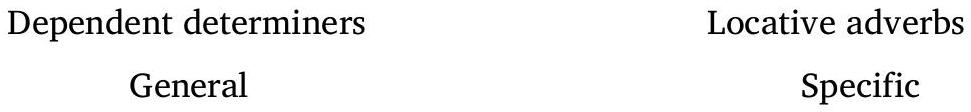
\includegraphics[width=\textwidth]{2025_09_03_818715438e96f16321bbg-056}
\end{center}
\end{figure}

\begin{table}[h]
\begin{center}
\captionsetup{labelformat=empty}
\caption{Table 18. Demonstratives}
\begin{tabular}{|l|l|l||l|l|l|l|l|}
\hline
Person & Proximal & Distal & Proximal & Distal & Proximal & Distal & Remote \\
\hline
sing. & \(d i\) & \(d e\) & handi & hande & handelle & handella & handello \\
\hline
pl. & \(r i\) & \(r e\) &  &  &  &  &  \\
\hline
\end{tabular}
\end{center}
\end{table}

The dependent determiners modify a head noun. Note the examples below:

\begin{center}
\begin{tabular}{|l|l|l|l|l|l|l|}
\hline
\multirow[t]{4}{*}{(117)} & Patke'a & de & enkohm &  & \(e^{\prime} a\) &  \\
\hline
 & patke'a & de & e-n-kohma &  & \(e^{\prime} a\) &  \\
\hline
 & female & that & \(3 \mathrm{~s}-3 \mathrm{~s}-\) hit &  & him &  \\
\hline
 & \multicolumn{6}{|l|}{'That girl hit me.'} \\
\hline
\multirow[t]{2}{*}{(118)} & Musti tuari &  & re & sukni &  & o'a \\
\hline
 & \multicolumn{6}{|l|}{'Those young men must like you.'} \\
\hline
\multirow[t]{3}{*}{(119)} & Krei di &  & inponni &  &  &  \\
\hline
 & church & this & big &  &  &  \\
\hline
 & \multicolumn{2}{|c|}{} &  &  &  &  \\
\hline
\end{tabular}
\end{center}

They may also combine with 'ha' and become the non-human free pronoun: See §3.2.1.5.

\begin{center}
\begin{tabular}{|l|l|l|l|l|l|}
\hline
\multirow[t]{3}{*}{(120)} & Om & Meki & gaha-ni & hadi &  \\
\hline
 & Uncle & Meki & possession-POS & this &  \\
\hline
 & \multicolumn{5}{|l|}{'This is Uncle Meki's possession.'} \\
\hline
\multirow[t]{3}{*}{(121)} & Hare & honnona & ra-kwieta & kok-koi. &  \\
\hline
 & They & all & 3 p -guess & RDP-riddle &  \\
\hline
 & \multicolumn{5}{|l|}{'They all guessed the riddle.'} \\
\hline
\multirow[t]{4}{*}{(122)} & Ra-tlin- & hade & de & ra-m-ta'at & wenna. \\
\hline
 & ra-tlina & hade & de & ra-m-ta'ata & wenna \\
\hline
 & 3p-hear & that & then 3p-STAT-afraid &  & dead \\
\hline
 & \multicolumn{5}{|l|}{'When they heard that they were scared to death.'} \\
\hline
\end{tabular}
\end{center}

The locative adverbs indicate location near or far. General locative demonstratives occur throughout narrative discourse. Specific locative demonstratives are very rare in narrative discourse but occur more frequently in procedural texts.

\begin{center}
\begin{tabular}{lll}
(123) & \begin{tabular}{l}
Yan mumkekla \\
yana mu-m-keka-la \\
do not 2s-STAT-see PREP \\
'Do not look over here.' \\
\end{tabular} & \begin{tabular}{l}
handi \\
handi \\
here \\
\end{tabular} \\
(124) & \begin{tabular}{l}
Ampatiawu \\
a-m-wa-tiawu \\
\end{tabular} & \begin{tabular}{l}
hande \\
hande \\
\end{tabular} \\
 & 'pe-1pe-MULT come from & there \\
 & 'We come from there.' &  \\
\end{tabular}
\end{center}

The independent determiners, non-human pronouns and locative pronouns may be modified by the enclitic na when occurring in questions. This enclitic can also occur in lists of objects as it does in §3.6.2.7 example (316).

\begin{center}
\begin{tabular}{|l|l|}
\hline
\multirow[t]{4}{*}{(125)} & O-m-la'a toko di-na? \\
\hline
 & o-m-la'a toko di-na \\
\hline
 & 2 s -2s-go store this-QU \\
\hline
 & 'Are you going to this store?' \\
\hline
\multirow[t]{4}{*}{(126)} & Omdyella \\
\hline
 & o-m-dena-la \\
\hline
 & 2 s -2s-stay-PREP Ody that-QU \\
\hline
 & 'Did you just come from Ody's?' \\
\hline
\multirow[t]{3}{*}{(127)} & O-gaha-mu \\
\hline
 & 2 s -possession-POS \\
\hline
 & 'Is this yours?' \\
\hline
\multirow[t]{4}{*}{(128)} & Mi-wo-tel-mi \\
\hline
 & mi-wo-telu-mi \\
\hline
 & 2 p -fruit-three-2p \\
\hline
 & 'Are you three taking that?' \\
\hline
\multirow[t]{4}{*}{(129)} & Hamto'a \\
\hline
 & ha-m-to'a \\
\hline
 & 3s-STAT-old \\
\hline
 & 'The old man ordered you to stand-up here?' \\
\hline
\multirow[t]{3}{*}{(130)} & Patke'a ri \\
\hline
 & \multirow{2}{*}{female these 3p-MULT-stay behind 'These women were left behind.'} \\
\hline
 &  \\
\hline
(131) & Krei di inponni church this big 'This church is big' \\
\hline
\multirow[t]{4}{*}{(132)} & ha-di \\
\hline
 & Om Meki \\
\hline
 & Om Meki \\
\hline
 & 'This one is Om Meki's' \\
\hline
\multirow[t]{4}{*}{(133)} & Mumkek \\
\hline
 & mu-m-keka \\
\hline
 & 2 s -STAT-see \\
\hline
 & 'Look at that!' \\
\hline
\end{tabular}
\end{center}

\begin{center}
\begin{tabular}{llll}
(134) & \begin{tabular}{l}
Yan mumkek \\
yana mu-m-keka la la han-di \\
do not 2s-STAT-see at \\
\end{tabular} & \begin{tabular}{l}
han-di \\
here \\
\end{tabular} &  \\
'Do not look here.' &  &  &  \\
(135) & \begin{tabular}{l}
A-m-pa-tiawu \\
a-m-wa-tiawu \\
\end{tabular} & \begin{tabular}{l}
han-de \\
1pe-1pe-MULT-come from \\
'We come from there.' \\
\end{tabular} & han-de \\
 &  &  &  \\
\end{tabular}
\end{center}

\subsection*{3.3 Adjectives}
Although many of the words that we consider adjectives in English occur as stative verbs in Luang, there is a small set of adjectives in Luang that follows the noun and modify it (see NP in §4.1). A number of these can also function as stative verbs when the pronominal prefix set is attached. Some can also function as predicates in semi-verbal and non-verbal clauses (see §6.4.2). Some of these can also be nominalized. The adjectives are often modified by the \(p\) or \(m\) (see §3.6.1.5) stative marker or the involuntary \(k\) (see §3.6.1.4). They are also often reduplicated.

\begin{center}
\begin{tabular}{|l|l|l|l|}
\hline
 & Adjectives & Stative Verb & Noun \\
\hline
\multirow[t]{3}{*}{(136)} & wehla m-nar-narta & na-m-nar-narta &  \\
\hline
 & knife STAT-RDP-sharp & 3s-STAT-RDP-sharp &  \\
\hline
 & 'sharp knife' & 'it is sharp' &  \\
\hline
\multirow[t]{3}{*}{(137)} & koka m-nur-nuhru & na-m-nur-nuhru &  \\
\hline
 & cloth STAT-RDP-silky & \(3 s\)-STAT-RDP-silky &  \\
\hline
 & 'silky cloth' & 'it is silky' &  \\
\hline
\multirow[t]{3}{*}{(138)} & ihru k-deha & na-k-deha & k-deha-ni \\
\hline
 & chest INVOL-dirty & 3 s -INVOL-dirty & INVOL-dirty-POS \\
\hline
 & 'sinful' (lit. dirty chest) & 'it is dirty' & 'dirt' \\
\hline
\multirow[t]{3}{*}{(139)} & ralam-ni werta-werta & \(n\)-werta &  \\
\hline
 & insides-POS RDP-heavy & \(3 s\)-heavy &  \\
\hline
 & 'worried' (lit. heavy insides) & 'it is heavy' &  \\
\hline
\end{tabular}
\end{center}

There is a small set of adjectives which function as quantifiers (see §3.5.3). These include:

\begin{center}
\begin{tabular}{|l|l|l|l|}
\hline
\multirow[t]{11}{*}{(140)} & harahu & 'many' &  \\
\hline
 & inpona & 'much' &  \\
\hline
 & honnona & 'all' &  \\
\hline
 & kuku'a & 'small bit' &  \\
\hline
 & oke'a & 'little bit' &  \\
\hline
 & ida-woru & 'one or two' &  \\
\hline
 & nenena & 'one or two' &  \\
\hline
 & тотиои & 'all' &  \\
\hline
 & rehenu & 'more than' &  \\
\hline
 & etamni & 'many' &  \\
\hline
 & lawna & 'much' &  \\
\hline
\multirow[t]{4}{*}{(141)} & La'pa & ra-wel-niana & oke'a \\
\hline
 & La'pa & ra-weli-nana & oke'a \\
\hline
 & Then & 3p-buy-ABIL & little \\
\hline
 & \multicolumn{3}{|c|}{'Then they went and bought some provisions.'} \\
\hline
\end{tabular}
\end{center}

(142) Noka a-wuwlu de sawra harahu\\
then 1 s -dive then seaweed lots\\
'When I dove there was lots of seaweed.'\\
Some of these can function as indefinite pronouns:\\
(143) Noka honnona rewre'wa ra-woka

Noka honnona re'wa-re'wa ra-woka\\
Then all RDP-together 3p-gather\\
'Then they all gathered together.'\\
(144) Demade honnona ra-mtatna.

Then all 3s-sat\\
'Then they all sat.'\\
(145) Ra-wkikni-ra-plialin momuouwa\\
ra-kikni-ra-plialni mou-mou-wa\\
3p-float-3p-float RDP-all-PERF\\
'Every single one floated away.'\\
Compound adjectives occur in ritual speech (see §9.5). They are formed when several adjectives combine together in a word pair or phrase, sometimes with other word classes as well, resulting in one overall meaning. Although the word pair is made up of adjectives, they tend to function as predicate in semi-verbal clauses (see §6.4).\\
(146) La'pa a-m-ler-la m-to'a-p-pe'a nih-tuini-morti-hamra

Till 1pi-1pi-reach-to STAT-old-STAT-old teeth-fallen-hair-white\\
'Till we become very old.'\\
(147) Me mel-u'uta-mel-kautu

And night-dark-night-thick\\
'And it was pitch black out.'\\
Other word class roots including precategoricals can be reduplicated to form adjectives.\\
(148) gai-ni mokla-mokla\\
face-POS RDP-smoke\\
'dizzy'\\
(149) pon-pona

RDP-blind (verb)\\
'grey'\\
(150) wa-wahra

RDP-clear (verb)\\
'white'

\subsection*{3.4 Adverbs}
Adverbs modify the verbs. They generally follow the verbs they modify (see §5) but this can occur elsewhere for reasons of topicalization or emphasis (see §7.1.4.1). They are also used to indicate tense and aspect (see §3.6.2.1). Some can also function as predicates in semi-verbal clauses (see §6.4).\\
(151) to'a 'only/just'\\
yeherto'a 'all the more'\\
toto'a 'completely'\\
wali 'also'\\
oleka 'already'\\
ma'ta 'not yet'

\begin{center}
\begin{tabular}{|l|l|l|l|l|l|l|}
\hline
\multirow{3}{*}{} & meha & 'only' & \multicolumn{4}{|c|}{} \\
\hline
 & emkadi/de & 'like this/that' &  &  &  &  \\
\hline
 & rewre'wa & 'together' &  &  &  &  \\
\hline
\multirow[t]{4}{*}{(152)} & Ai-lier-nana & emna & ida & meha &  &  \\
\hline
 & a-u-ler-nana & emna & ida & meha &  &  \\
\hline
 & 1s-get-ABIL & eel & one & only &  &  \\
\hline
 & \multicolumn{5}{|l|}{'I got only one eel.'} &  \\
\hline
\multirow[t]{4}{*}{(153)} & A-niar & to'a & pola & to'ora & mot-mota & ida \\
\hline
 & A-u-nairi & to'a & pola & to'ora & mota-mota & ida \\
\hline
 & 1 s -1s-wear & only & pants & cut-off & RDP-green & one \\
\hline
 & \multicolumn{6}{|l|}{'I wore only a green pair of cut-off pants.'} \\
\hline
\multirow[t]{4}{*}{(154)} & A-g-al & to-to'a &  & a-ralm-u & \(l a^{\prime}\) &  \\
\hline
 & A-u-al & to'a-to'a &  & a-ralma-u & \(l a^{\prime}\) &  \\
\hline
 & 1 s -1s-give & RDP-truly &  & insides-POS & at &  \\
\hline
 & \multicolumn{6}{|l|}{'I worked really hard at school.'} \\
\hline
\multirow[t]{4}{*}{(155)} & Na-kot & wali-a & pena & e-n-pairi &  &  \\
\hline
 & Na-kota & wali-a & репа & e-n-pairi &  &  \\
\hline
 & 3 s -said & also-OBJ & later & 3s-3s-pay &  &  \\
\hline
 & \multicolumn{6}{|l|}{'He also said that later he would pay.'} \\
\hline
\end{tabular}
\end{center}

\subsection*{3.4.1 Adverbs as predicates}
Several of the adverbs such as emkade 'like that', emkadi 'like this', and rewre'wa 'together' can also stand as predicates in the absence of the verb they normally modify. Emkade also can function as part of a conjunction as in emkade pede 'because of that therefore' (see §6.4.9).

\begin{center}
\begin{tabular}{lccc}
N-wa-haur & nohora & emkade-emkadi-la & in-ni-am-ni \\
n-wa-hauru & nohora & emkade-emkadi-la & ina-ni-ama-ni \\
3s-MULT-gossip & about & like that-like this-about & mother-POS father-POS \\
'He talked about what was happening with his mother and father.' &  &  &  \\
\end{tabular}
\end{center}

\begin{center}
\begin{tabular}{lllll}
R-hi'a & krita & kerna, & rhi'a & emkadi: \\
3p-make & octopus & dry, & 3p-make & like this \\
'When you make dried octopus you make it like this:' &  &  &  &  \\
\end{tabular}
\end{center}

\begin{center}
\begin{tabular}{llll}
Pa lera-lera emkade & ma-maini \\
pa lera-lera emkade & mai-maini \\
for day-day like that & RDP-only \\
'Every day it was just like that.' &  \\
\end{tabular}
\end{center}

(159)

Pa \(\quad\) r-mai de, \(\quad\) rewrewa\\
pa \(\quad\) r-mai de, \(\quad\) rewa-rewa\\
for 3p-come that, \(\quad\) RDP-together\\
'When they came, (they came) together.'

\subsection*{3.5 Quantifiers, classifiers and numbers}
\subsection*{3.5.1 Noun quantifiers}
Plurality is often not indicated in Luang when it is not in focus. At other times it is indicated by the plural determiners ri (close) and re (far), see §3.2.2. Sometimes there is modification by specific numbers and at other times there is reduplication of whole words indicating plurality but a vagueness of exact number.

\begin{center}
\begin{tabular}{|l|l|}
\hline
(160) & Yohia'a re thing those 'those things' \\
\hline
(161) & \multirow{2}{*}{\begin{tabular}{l}
Yehudi ri let-ni \\
re Yehudi ri leta-ni re Yehudi these village-POS those 'Those villages of these Yehudi.' \\
\end{tabular}} \\
\hline
 &  \\
\hline
(162) & Ri-mor-miori re \(r\)-peh mut-liawna Ri-mori-mori re r-peha mutu-lawna people-RDP-live those 3p-grow group-large 'Those people grew to be a great multitude.' \\
\hline
(163) & \begin{tabular}{l}
Limni \\
woru lima-ni woru five-POS two 'two hands' \\
\end{tabular} \\
\hline
(164) & А-уе'y-u a-yei-'u My-uncle-POS 'My uncle's house.' \\
\hline
(165) & Musa lir-ni re'e-ni wolim-ni Musa lira-ni re'e-ni wolima-ni Musa words-POS time-POS five-POS 'Musa's words for the fifth time.' \\
\hline
\end{tabular}
\end{center}

When reduplication is used to indicate plurality it indicates 'many' but not the specific number. It can also indicate the individuality within plurals.\\
(166) o'ta-o'ta\\
head-head\\
'leaders'\\
(167) leta-leta\\
village-village\\
'many villages'\\
(168) hia'a-hia'a\\
what-what\\
'whatever/anything.'\\
(169) he'a-he'a\\
who-who\\
'whoever'\\
(170) meha-meha\\
alone-alone\\
'each one individually'\\
(171) rima-rima\\
each-each\\
'each one'

\subsection*{3.5.2 Numbers}
The Luang counting system is quite complex with different ways of counting depending on the object being counted, as well as discourse considerations.

\subsection*{3.5.2.1 General numbers}
Listed below is the counting system used in school for math and for measuring weights and distances, money, etc. A native speaker suggested that it is a more recent system produced as a result of Indonesian influence on the Luang culture. The 'wo' in each of the numbers comes from the classifier wo'a 'fruit'. The wehrani in each of the numbers means 'its-pieces'.

\begin{center}
\begin{tabular}{|l|l|l|}
\hline
1 & ida &  \\
\hline
2 & woru \({ }^{45}\) &  \\
\hline
3 & wotelu &  \\
\hline
4 & wogata &  \\
\hline
5 & wolima &  \\
\hline
6 & wonema &  \\
\hline
7 & wo'itu &  \\
\hline
8 & wo'awa &  \\
\hline
9 & wosiewa &  \\
\hline
10 & termida &  \\
\hline
11 & termida wehrani ida & 'ten added one' \\
\hline
12 & termida wehrani woru & 'ten added two' \\
\hline
13 & termida wehrani wotelu & 'ten added three' \\
\hline
14 & termida wehrani wogata & 'ten added four' \\
\hline
20 & teramporu & 'ten two' \\
\hline
21 & teramporu wehrani ida & 'ten added one' \\
\hline
22 & teramporu wehrani woru & 'ten added two' \\
\hline
23 & teramporu wehrani wotelu & 'ten added three' \\
\hline
24 & teramporu wehrani wogata & 'ten added four' \\
\hline
30 & terampotelu & 'ten three' \\
\hline
40 & terampogata & 'ten four' \\
\hline
50 & terampolima & 'ten five' \\
\hline
100 & rahu ida & 'hundred one' \\
\hline
200 & rahu woru & 'hundred two' \\
\hline
1000 & riwnu ida & 'thousand one' \\
\hline
2000 & riwnu woru & 'thousand two' \\
\hline
\end{tabular}
\end{center}

\subsection*{3.5.2.2 Numbers in trading}
The following counting system is used for counting things, such as in the selling or trading of items like eggs, books etc.

1-9 are the same as above

\begin{center}
\begin{tabular}{lll}
10 & hanulu 'ten' &  \\
11 & hanulu wehrani ida & 'ten added one' \\
12 & hanulu wehrani woru & 'ten added two' \\
13 & hanulu wehrani wotelu & 'ten added three' \\
20 & hanulu woru & 'ten two' \\
21 & hanulu woru wehrani ida & 'ten two added one' \\
22 & hanulu woru wehrani woru & 'ten two added two' \\
23 & hanulu woru wehrani wotelu & 'ten two added three' \\
\end{tabular}
\end{center}

\footnotetext{\({ }^{45}\) When modifying a pronoun, woru takes the form of ro'a.\\
Itro'a tsoliwut la hadiwa.\\
'We two live together from now on.'
}\begin{center}
\begin{tabular}{lll}
30 & hanulu wotelu & 'ten three' \\
40 & hanulu wogata & 'ten four' \\
50 & hanulu wolima & 'ten five' \\
60 & hanulu wonema & 'ten six' \\
100 & hanulu termida & 'ten ten' \\
200 & hanulu teramporu & 'ten twenty' \\
1000 & hanulu rahu ida & 'ten one-hundred' \\
2000 & hanulu rahu woru & 'ten two-hundred' \\
\end{tabular}
\end{center}

\subsection*{3.5.2.3 Counting fish}
The following counting system is to count fish. (Luang culture and commerce centers around the sea.)\\
1-9 are the same as above

\begin{center}
\begin{tabular}{|l|l|l|}
\hline
10 & ahwida & 'ten' \\
\hline
11 & ahwida wehrani ida & 'ten added one' \\
\hline
12 & ahwida wehrani woru & 'ten added two' \\
\hline
13 & ahwida wehrani wotelu & 'ten added three' \\
\hline
14 & ahwida wehrani wogata & 'ten added four' \\
\hline
20 & ahwu woru & 'ten two' \\
\hline
30 & ahwu wotelu & 'ten three' \\
\hline
40 & ahwu wogata & 'ten four' \\
\hline
50 & ahwu wolima & 'ten five' \\
\hline
100 & ahwu termida & 'ten ten' \\
\hline
200 & ahwu teramporu & 'ten twenty' \\
\hline
1000 & ahwu rahu ida & 'ten hundred one' \\
\hline
2000 & ahwu rahu woru & 'ten hundred two' \\
\hline
\end{tabular}
\end{center}

\subsection*{3.5.2.4 Counting sets}
The following system is for the counting of animals in which they count by tens only.

\begin{center}
\begin{tabular}{|l|l|l|}
\hline
10 & tali ida & 'one set' \\
\hline
20 & tali woru & 'two sets \\
\hline
30 & tali wotelu & 'three sets' \\
\hline
40 & tali wogata & 'four sets' \\
\hline
50 & tali wolima & 'five sets' \\
\hline
60 & tali wonema & 'six sets' \\
\hline
70 & tali wo'itu & 'seven sets' \\
\hline
80 & tali wo'awa & 'eight sets' \\
\hline
90 & tali wosiewa & 'nine sets' \\
\hline
100 & tali termida or tali hanulu & 'ten sets' \\
\hline
200 & tali hanulu woru & 'ten two sets' \\
\hline
1000 & tali rahu ida & 'hundred one sets' \\
\hline
2000 & tali rahu woru & 'hundred two sets' \\
\hline
\end{tabular}
\end{center}

\subsection*{3.5.2.5 Numbers used in discourse tracking}
The following counting system is used in discourse for tracking participant referents through a text. The first time the participants are referred to, the normal numbers \(1-10\) are used. After that however, when those participants are subsequently referred to the following number system is used.

1 de/di\\
2 rora

3 mantetelu\\
4 mandadata\\
5 manlimlima\\
6 mannemnema\\
7 mandiditu\\
Note the following examples of sentences occurring together in a particular discourse:\\
a. Patke'a ida n-ora muanke'a ida r-mehlima

Woman one 3 s -with male one 3 p -marry\\
'A woman and a man were married.'\\
b. R-rora a'na-ni muanke'a woru

3p-two child-POS man two\\
'The two of them had two children.'\\
c. R-rora am-ni Rettiau pede r-iwra Rettiau-Ru'ru-Rettiau-Lai

3p-two father-POS Rettiau therefore 3p-call Rettiau-My Strength-Rettiau-Strength\\
'Those two (children's) father's name was Rettiau, therefore they were called Rettiau-Ru'ru-Rettiau-Lai.'\\
a. Maran Leterwo'ora ida n-wawa Teti-Lai

Maran Leterwo'ora one 3s-name Teti-Lai\\
'There was a Maran Leterwo'ora named Teti-Lai'\\
b. Teti-Lai di n-waka Miru-Lewan nar-ni

Teti-Lai this-one 3s-asked-for Miru-Lewan sister-POS\\
'This Teti-Lai asked for Miru Lewan's sister.'\\
a. O'ta-ni-mat-ni ida a'na-ni muanke'a riy wo'itu head-POS-eye-POS one child-POS male people seven 'A leader had seven sons.'\\
b. N-karma riy mandiditu re pa ra-mno'a-ra-mrara 3s-attack people seven those till 3p-wound-3p-blood 'He attacked those seven people till they were wounded and bloodied.'

\subsection*{3.5.2.6 Ordinal numbers}
The ordinal numbers are used to refer to a certain participant position or rank in a given number of participants. In Luang the ordinal numbers are formed by the suffixation of the 3s possessive on the numbers.

1 id-ni\\
2 wor-nu\\
3 wotel-lu\\
4 wogat-ni\\
5 wolim-ni\\
6 wonem-ni\\
7 wo-itnu\\
(175) T-ni-atar lir-ni re'e-ni wotel-lu\\
ni-tatra lira-ni re'a-ni wotelu-lu\\[0pt]
NOM-law words- [time]-POS three-POS\\
'The third verse of the law.'\\
(176) Musa lir-ni re'e-ni wolim-ni

Musa lira-ni re'a-ni wolima-ni\\
Musa words-POS time-POS five-POS\\
'Musa's words for the fifth time.'

\begin{center}
\begin{tabular}{llllll}
(177) La'a wolan pen-puenu & wor-nu & di &  \\
 & at month RDP-full & two-POS & this \\
 & 'This whole second month.' &  &  \\
\end{tabular}
\end{center}

\subsection*{3.5.2.7 Fractions}
The word rehenu 'more than' is used to refer to one half or actually any amount which is between two whole numbers. Specific words for specific fractions do not exist.\\
(178) A-kuli' pa la'nana anni woru rehenu

1 s -school for reach year two more\\
'I went to college for more than two years.'

\subsection*{3.5.2.8 Compound numbers}
In ritual speech compound numbers are used. See §9.5 for further discussion of ritual speech.

\begin{center}
\begin{tabular}{lc}
ida-woru & woru-wotelu \\
one-two & two-three \\
'one or two/few' &  \\
\end{tabular}
\end{center}

riwnu- halli\\
thousands- many\\
'huge numbers'\\
The use of Luang numerals is decreasing. Indonesian numerals are usually substituted, especially numerals above 10. This may be due to several factors, one of them being that dealing with complicated numbers is rarely done within the culture but used more in trading with the outside world. School, and therefore mathematics, is learned in Indonesian. Also formulating Indonesian numerals may be less complicated than Luang ones

\subsection*{3.5.3 Indefinite quantifiers}
A closed set of adjectives functioning as quantifiers may modify nouns. Most of these can also function as indefinite pronouns when they stand alone (see §3.2.1.6).

\begin{center}
\begin{tabular}{|l|l|l|l|l|}
\hline
\multirow[t]{11}{*}{(179)} & harahu & 'many' &  &  \\
\hline
 & inpona & 'much' &  &  \\
\hline
 & honnona & 'all' &  &  \\
\hline
 & kuku'a & 'small bit' &  &  \\
\hline
 & oke'a & 'little bit' &  &  \\
\hline
 & ida-woru & 'one or two' &  &  \\
\hline
 & nenena & 'one or two' &  &  \\
\hline
 & тотиои & 'all' &  &  \\
\hline
 & rehenu & 'more than' &  &  \\
\hline
 & etamni & 'many' &  &  \\
\hline
 & lawna & 'much' &  &  \\
\hline
\multirow[t]{4}{*}{(180)} & \multicolumn{3}{|l|}{Noka honnona rewre'wa} & ra-woka \\
\hline
 &  & Noka honnona & re'wa-re'wa & ra-woka \\
\hline
 & Then all &  & RDP-together & 3p-gather \\
\hline
 & \multicolumn{4}{|l|}{'Then they all gathered together.'} \\
\hline
\multirow[t]{3}{*}{(181)} & \multicolumn{4}{|l|}{Demade honnona ra-mtatna.} \\
\hline
 & Then & all & 3 s -sat &  \\
\hline
 & \multicolumn{4}{|l|}{'Then they all sat.'} \\
\hline
\end{tabular}
\end{center}

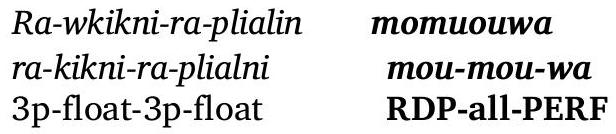
\includegraphics[max width=\textwidth, center]{2025_09_03_818715438e96f16321bbg-066}\\
'Every single one floated away.'

\subsection*{3.6 Verbs}
This section discusses pronominal prefixation of verbs as well as briefly discussing affixation and reduplication for inflectional and derivational purposes. Verbs can be derived from other word classes as well as from precategorical roots. The processes of prefixation and reduplication are valence changing devices. Cliticization indicates person, tense, aspect, and mode and emotional content.

\begin{table}[h]
\begin{center}
\captionsetup{labelformat=empty}
\caption{Table 19. Pronominal prefixation of verbs}
\begin{tabular}{|l|l|l|l|}
\hline
Proclitic & Prefix & Verb & Enclitic \\
\hline
Durative \(e\) - & Pronoun &  & Object marker \\
\hline
Instrument na- & Relative \(k\) - &  & Post verbal aux. \\
\hline
ema- & Non-intentional \(k\) - &  & Locative \\
\hline
 & Stative &  & Vocative \\
\hline
 & Multiple object &  & Reflexive \\
\hline
\end{tabular}
\end{center}
\end{table}

\subsection*{3.6.1 Prefixation}
Verbal prefixes in Luang include the pronominal prefix, relativizing prefix, non-intentional prefix, stativizer prefix, and multiple object prefix.

\subsection*{3.6.1.1 Pronominal prefixation of verbs}
All verbs except for predicates of semi and non-verbal clauses require pronominal prefixation. As stated above in §3.2.1.4 there are two classes of verbs. These are morphologically subcategorized by the affixation of the following pronominal markers. The parentheses in 2 s forms in the chart below indicate the high vowels which spread into the root of the verbs and take set 2 prefixes.

\begin{table}[h]
\begin{center}
\captionsetup{labelformat=empty}
\caption{Table 20. Pronominal prefixes}
\begin{tabular}{|llll|llll|}
\multicolumn{5}{c}{Set 1} & \multicolumn{4}{c}{Set 2} \\
\hline
1 s & \(u\) & 1 pe & \(m a\) & 1 s & \(u\) & 1 pe & \(m\) &  \\
 &  & 1 pi & \(t a\) &  &  & 1 pi & \(t\) &  \\
2 s & \(m u\) & 2 p & \(m i\) & 2 s & \(m(u)\) & 2 p & \(m(i)\) &  \\
3 s & \(n a\) & 3 p & \(r a\) & 3 s & \(n\) & 3 p & \(r\) &  \\
\hline
\end{tabular}
\end{center}
\end{table}

These pronominal prefix sets cannot be explained purely by phonological reasons, though phonological rules affect some words. Note the following minimal pairs.

\begin{center}
\begin{tabular}{|l|l|l|l|}
\hline
na-la'a & 'she/he walks' & \(n-l a^{\prime} a\) & 'she/he goes' \\
\hline
na-uhu & 'she has breasts' & n-uhu & 'he/she nurses (from mother)' \\
\hline
na-wenna & 'he/she is angry' & n-wenna & 'he/she kills' \\
\hline
na-mori & 'she gives birth' & n-mori & 'he/she lives' \\
\hline
na-werta & 'he/she considers' & n-werta & 'he/she is heavy' \\
\hline
na-turu & 'she lets down (milk)' & n-turu & '(rain) falls' \\
\hline
na-'atu & 'he/she gives advice' & n-atu & 'he/she knows' \\
\hline
\end{tabular}
\end{center}

\begin{center}
\begin{tabular}{llll}
па-репи & 'he/she makes full' & n-penu & 'it is full' \\
па-kerna & 'he/she makes dry' & n-kerna & 'it is dry' \\
\end{tabular}
\end{center}

The only phonological limitation affecting the prefix sets occurs when a verb begins with a consonant cluster. These clusters are generally the result of a verb being derived from another word class or precategorical, loan words, or added prefixes (stative etc.). When this happens the verb stem must take set 1 prefixes. This is because in Luang there cannot be three consonants in a row. If these were to take the second set, there would be three contiguous consonants occurring.

\begin{center}
\begin{tabular}{lll}
(183) & \begin{tabular}{l}
na-krui \\
3s-spit \\
\end{tabular} & (not n-krui) \\
 & 'she spits (on)' &  \\
(184) & \begin{tabular}{l}
na-sterika \\
3s-iron \\
\end{tabular} & (not n-sterika) \\
 & 'she irons (it)' &  \\
(185) & \begin{tabular}{l}
na-prowta \\
3s-thin \\
\end{tabular} &  \\
 & 'he/she is thin' & (not n-prowta) \\
\end{tabular}
\end{center}

The reasons for the use of these verb sets cannot be drawn along the lines of transitivity in the sense that transitive verbs always take one prefix set and stative and other intransitives always take another. Each of these verb types can occur with both prefix sets.

\begin{table}[h]
\begin{center}
\captionsetup{labelformat=empty}
\caption{Table 21. Transitive verb prefixes}
\begin{tabular}{|l|l|l|l|}
\hline
\multicolumn{2}{|c|}{Set 1} & \multicolumn{2}{|c|}{Set 2} \\
\hline
na-tona & 'it soaks' & n-ala & 'he gives' \\
\hline
na-woka & 'he gathers (wood)' & n-taili & 'he weighs' \\
\hline
na-dairi & 'he gathers (seaweed)' & n-keni & 'he puts' \\
\hline
na-kiri & 'she holds (child)' & n-ihi & 'he bites' \\
\hline
na-gari & 'he suns (seaweed)' & n-riki & 'he rips' \\
\hline
\end{tabular}
\end{center}
\end{table}

(186) La'pa muanke'a r-hi'a owa'ana puou auw-nu Then man \(\boldsymbol{3 p}\)-made again boat board-POS 'Then the men made/fixed the board again.' (Transitive-set 2 prefix)\\
(187) Mere mak-ler de de a-'u-kleha lawra-raini iskola. But when-day that then 1 s - 1 s -did not have cloth-clothes school 'But at that time I did not have school clothes.' (Transitive-set 1 prefix)\\
(188) A-g-ora tungguru-a Paulus m-torna iskola Lgona. \(1 \mathrm{~s}-1 \mathrm{~s}\)-with teacher-OBJ? Paulus 1pe-hold school Lgona 'I and teacher Paulus were the heads of the school in Lgona.' (Transitive-set 2 prefix)\\
(189) Ami edon ma-mkek-nan ma'ta noha Apnu. We not 1pe-see-ABIL yet island Apnu 'We had not yet been able to see/seen the island of Ambon.' (Transitive-set 1 prefix)

\begin{table}[h]
\begin{center}
\captionsetup{labelformat=empty}
\caption{Table 22. Transitivity chart for intransitives}
\begin{tabular}{|l|l|l|l|}
\hline
\multicolumn{2}{|c|}{Set 1} & \multicolumn{2}{|c|}{Set 2} \\
\hline
na-nauru & 'she chews (betelnut)' & n-della & 'he stays' \\
\hline
na-krehena & 'she bares down' & n-hargota & 'he goes out' \\
\hline
na-he'i & 'he plays' & n-lola & 'he goes by' \\
\hline
na-la'a & 'he walks' & п-егnu & 'he goes down' \\
\hline
na-nina & 'he sleeps' & п-ra'a & 'he goes on shore' \\
\hline
na-kowa & 'he is face down' & n-warna & 'he takes a breath' \\
\hline
\end{tabular}
\end{center}
\end{table}

(190) Noma ma-wali-a liwu ralam-ni.

Then 1pe-return-OBJ harbor inside-POS\\
'Then we returned to the harbor.' (Intransitive-Set 1)\\
(191) A-m-ton-la noha Tepa.

1pe-1pe-float-at island Tepa\\
'We harbored at the island of Tepa.' (Intransitive-Set 2)\\
(192) R-rora ra-wlar-wia\\
r-rora ra-wlari-wa\\
3p-two 3p-run-PERF\\
'The two of them ran.' (Intransitive-Set 1)

\begin{table}[h]
\begin{center}
\captionsetup{labelformat=empty}
\caption{Table 23. Transitivity chart for statives}
\begin{tabular}{|l|l|l|l|}
\hline
\multicolumn{2}{|c|}{Set 1} & \multicolumn{2}{|c|}{Set 2} \\
\hline
па-таи & 'he is tired' & n-maha & 'he is very tired' (panting) \\
\hline
па-ариарпи & 'she is pregnant' (barely pregnant) & n-malanu & 'she is very pregnant' (stomach is large) \\
\hline
\end{tabular}
\end{center}
\end{table}

(193) А'-apn-u na-mehra.

My-stomach 3s-sick\\
'My stomach hurts' (Stative-Set 1)\\
(194) Dewade a-g-hedma.

Dewade a-u-hedma\\
Then 1s-1s-shock\\
'Then I was shocked.' (Stative-Set-2)\\
(195) Noha n-ker-kerna.

Noha n-kerna-kerna\\
island 3s-RDP-dry\\
'The island is dry' (Stative-Set 2)\\
(196) Patke' de e-na-'apnu\\
female that DUR-3s-pregnant\\
'That woman is pregnant.' (Stative-Set 1)

So the issue here does not seem to be phonology or transitivity per \(\mathrm{se}^{46}\). The structural difference between the two sets is that Set 2 prefixes do not have a final vowel as do Set 1 prefixes. These final vowels are \(/ a /\) except for 2 s and 2 p where it is \(/ u /\) and \(/ i /\) respectively \({ }^{47}\). When the first prefix set occurs with general intransitive verbs it seems to imply instrument used to accomplish the verb.

\begin{center}
\begin{tabular}{llll}
(197)\begin{tabular}{llll}
irnu & 'nose' & \(n a-i r n u\) & 'she/he smells' (lit. to use/take nose) \\
 & \(h e ' i\) & 'toy' & \(n a-h e\) 'i \\
\end{tabular} & 'she/he plays' (lit. to use/take toy) &  &  \\
 & \(u h u\) & 'breast' & \(n a-u h u\) \\
\end{tabular}
\end{center} 'she nurses' (lit. she uses/gives breast)

In intransitive stative verbs it implies the possession of an object which results in a state or defines it.\\
(198) -арпи 'stomach' па-арпи 'she is pregnant' (lit. she has stomach)\\
uhu 'breast' na-uhu 'she is pregnant' (lit. she has breasts)\\
In transitive verbs it seems to act as a causative. Elsewhere in the language \(/ a /\) is a clitic indicating object. / \(a /\) is also the precategorical root of the word 'to take' and 'to give'. It is interesting to note that Ambonese Malay, which is similar to Luang in a number of areas, uses 'give' in the construction of causatives. /a/ is also used in instrumental constructions (see §5.2.2.2).\\
(199) tona 'soak' na-tona 'he/she causes to soak'\\
woka 'gather' na-woka 'he/she causes to gather'\\
gari 'dry-in-sun' na-gari 'he/she causes to dry-in-sun'

\subsection*{3.6.1.2. K-Prefix for relativization}
The prefix \(\boldsymbol{k}\) - has a relativizing function which lowers transitivity. The relative pronoun is maka 'the one/thing who/which' (see §3.2.1.7). When the head of the relative clause which precedes the relative pronoun and the subject of the verb being relativized are coreferential than a \(k\)-prefix replaces the required pronominal prefix on the verb. When they are not the same participant then the pronominal prefixation will indicate the actor. The relative clause is explained further in §7.2.

Note the following examples:

\footnotetext{\({ }^{46}\) Though one could postulate that set 1 is syntactically more highly active or transitive than set 2 : if the / \(a /\) does indeed indicate object, then it indicates another argument on the verb. However, the object is not in the direct object slot, but as an instrument used to perform the verb. With set 2 verbs this /a/ does not occur and the action directly affects the direct object or actor as undergoer. With set 1 verbs there is one step between the two, an instrument or object, which makes the action less highly active.\\
\({ }^{47}\) Another interpretation could be that there is only 1 set of verb prefixes and that [ \(u\) ] and [ \(i\) ] are allophones of an object marker / \(a / \mathrm{l}[u]\) occurring in 2ps and [i] 3ps in order to more closely mirror the free pronoun. The advantage of this interpretation would be to narrow down to one prefix set. The disadvantage would be to try and explain exactly how \([u]\) and \([i]\) can be allophones of \(/ a /\). However, if they are allophones of \(/ a /\) it might explain why this context is the only one in the whole language, including across grammatical word boundaries, where the high vowels never spread. An underlying / \(a /\) would stop this process from occurring since it does this in all other contexts.
}\begin{table}[h]
\begin{center}
\captionsetup{labelformat=empty}
\caption{Table 24. Relative clause}
\begin{tabular}{|ll|}
\hline
Clause & Relative Clause \\
na-tiaka & maka \(\boldsymbol{k}\)-tiaka \\
3s-guard & one who REL-guard \\
'He guards' & 'The one who guards.' \\
\(n\)-hakra & maka \(\boldsymbol{k}\)-hakra \\
3s-divide & one who REL-divides \\
'He divides' & 'The one who divides.' \\
\hline
\end{tabular}
\end{center}
\end{table}

\begin{center}
\begin{tabular}{llllllll}
Uplerlawna & ed & maka & \(\boldsymbol{k}-h i^{\prime}\) & \(a^{\prime}-a^{\prime} m-u\) & de & muan & die. \\
Uplerlawna & eda & maka & \(\boldsymbol{k}-h i^{\prime} a\) & \(a^{\prime}-a m a-{ }^{\prime} u\) & de & muanu & de \\
God & is who & REL-made & my-father-POS & that & man & that &  \\
'God is the one who made that man my father.' &  &  &  &  &  &  &  \\
\end{tabular}
\end{center}

\begin{center}
\begin{tabular}{|l|l|l|l|l|l|l|l|l|}
\hline
Riy & maka & edon & ka-m-ta'ata &  & \multicolumn{3}{|c|}{Uplerlawna-Mempulwatnu} & lir-ni-tun-nu \\
\hline
Riy & maka & edonna & ka-m-ta'ata &  & Uplerlawna-Mempulw &  & atnu & lira-ni-tunu-nu \\
\hline
People & who & do not &  & REL-STAT-fear & God-God &  & word-POS-word &  \\
\hline
\multicolumn{9}{|l|}{'People who do not fear God's word.'} \\
\hline
Hari & honnona & ed & maka & \(\boldsymbol{k}\)-tutg-a & talla & \(l a^{\prime}\) &  & it-mor-miori-ni \\
\hline
Hari & honnona & eda & maka & \(k\)-tutu-a & talla & \(l a^{\prime}\) &  & it-mori-mori-ni \\
\hline
These & all & are & what & REL-point-OBJ & road & for &  & our-RDP-life-POS \\
\hline
\multicolumn{9}{|l|}{'All these things are what point out the road for our life.'} \\
\hline
\end{tabular}
\end{center}

\subsection*{3.6.1.3 Non-intentional \(k\) - prefix}
Another \(k\) - prefix occurs with a closed set of verbs. These seem to signal non-intentionality or involuntary action.

\begin{center}
\begin{tabular}{ll}
na- \(k\)-lierta & 'it is too tight' \\
na- \(k\)-dielma & 'it is deep' \\
na- \(k\)-deha & 'it is dirty' \\
na- \(k\)-towru & 'it is spilled' \\
\end{tabular}
\end{center}

\(N\)-heduma na-mkeka riy mati di pa na-k-niaun- nande inni 3 s-shocked 3 s -see person dead this so 3 s -INV-shout? -DUR mother 'He was shocked to see this dead person so he shouted and shouted, "Mother!"'

\begin{center}
\begin{tabular}{lllll}
Oktovina & morat-nu & \(n\)-ma & \(n a-k\)-niun-la & te'ena \\
Oktovina & hair-POS & 3s-DIR & 3s-INV-fall-around & pole \\
\end{tabular}
\end{center}

'Oktovina's hair came and encircled the pole.'

\subsection*{3.6.1.4 Stativizer}
Some roots can take the stative marker \(\boldsymbol{m}\)-. Pronominal prefixes are then added producing a stative verb. ( \(/ m /\) becomes \([p]\) preceding \(/ l /\) and \(/ p /\) (see §2.5).\\
(206) na-p-lara\\
\(3 s\)-STAT-hunger\\
'He is hungry.'\\
(207) na-p-lola

3s-STAT-straight\\
'It is true.'

\begin{center}
\begin{tabular}{|l|l|}
\hline
(208) & \begin{tabular}{l}
na-m-no'a \\
3s-STAT-a sore \\
'It has a wound.' \\
\end{tabular} \\
\hline
(209) & \begin{tabular}{l}
na-m-ta'ata \\
3s-STAT-afraid \\
'He is scared.' \\
\end{tabular} \\
\hline
(210) & \begin{tabular}{l}
Ra-tlin- hade de ra-m-ta'at wenna. \\
ra-tlina hade de ra-m-ta'ata wenna \\
3p-hear that then 3p-STAT-afraid dead \\
'When they heard that they were scared to death.' \\
\end{tabular} \\
\hline
(211) & \begin{tabular}{l}
La'pa a-m-ler-la m-to'a-p-pe'a \\
Till 1pi-1pi-reach-to STAT-old man-STAT-old woman \\
'Till we become old with white hair and falling teeth.' \\
\end{tabular} \\
\hline
(212) & \begin{tabular}{l}
Nhi'pa l-lawan-wa mere na-m-no'a-na-m-rara \\
almost 3s-big-PERF but 3s-STAT-wound-3s-STAT-blood \\
'He was almost grown but he was wounded.' \\
\end{tabular} \\
\hline
\end{tabular}
\end{center}

\subsection*{3.6.1.5 Multiple object prefix}
The prefix wa indicates indiscriminateness of action. This includes reciprocal type action where there are two actors involved, as well as continuous, repetitive or iterative action where the action goes on and on or is repeated over and over again.

\begin{center}
\begin{tabular}{|l|l|l|}
\hline
(213) & r-wa-dup-la &  \\
\hline
 & 3p-MULT-fight-loc &  \\
\hline
 & 'They fight each other.' & Reciprocal \\
\hline
(214) & \(r\)-wa-haka &  \\
\hline
 & 3p-MULT-search & Continuous \\
\hline
(215) & r-wa-kini &  \\
\hline
 & 3p-MULT-kiss &  \\
\hline
 & 'They kiss.' & Reciprocal \\
\hline
(216) & n-wa-tutu &  \\
\hline
 & 3s-MULT-point-out &  \\
\hline
 & 'He teaches' & Iterative \\
\hline
\end{tabular}
\end{center}

Note the following sentence examples:

\begin{center}
\begin{tabular}{|l|l|l|l|}
\hline
(217) & \multicolumn{3}{|l|}{\multirow{2}{*}{Seri n-wa-hora kenkua de Seri 3s-MULT-scold child that 'Seri scolds and scolds that child.'}} \\
\hline
 &  &  &  \\
\hline
(218) & \multicolumn{3}{|l|}{\multirow{2}{*}{\begin{tabular}{l}
It-ro' ta-wa-hernu rai-ni 1p-two 1pi-MULT-change clothes-POS 'The two of us exchange clothes' \\
A-wu-a-haka a-mehli'm-u A-u-wa-haka a-mehlima-'u 1 s -1s-MULT-search my-marriage-POS 'I am trying to find a way to get married.' \\
\end{tabular}}} \\
\hline
(219) &  &  &  \\
\hline
(220) & \begin{tabular}{llll}
Na'nama & n-or & mam-ni & n-wa-trom \\
Na'nama & n-ora & mama-ni & n-wa-troma \\
Just & 3s-with & mother-POS & 3s-MULT-meet \\
'Just now she and her mother meet and kiss and kiss.' &  &  &  \\
\end{tabular} &  &  \\
\hline
 &  &  &  \\
\hline
\end{tabular}
\end{center}

\subsection*{3.6.2 Cliticization}
The monosyllabic and disyllabic morphemes which occur verb initially and finally are considered to be clitics rather than prefixes and suffixes because in many cases other word classes can be inserted between them and the verbs that they modify. The proclitics \(e\) - and ema-, and the enclitics \(-w a\), and \(-a\) are in this category. The modal, aspect markers which are disyllabic are also analyzed as clitics since some can stand alone in other contexts. And the same verbs may occur with or without these clitics with only a change in aspect, or modality but not in meaning or valency.

\subsection*{3.6.2.1 Tense-Aspect-Mood (TAM)}
Specific time in Luang is not considered very important or distinctive. The word for 'day' lera can mean 'sun, season, day, hour, time'. It is not strange then that tense would be of less consideration than aspect and mood which tend to communicate more about the speakers feelings about a certain event, than the time in which it occurred. In Luang, a large number of clitics and some words are used to indicate the emotional content of events. The chart below shows each type, however the discussion below will focus only on the clitics.

\begin{table}[h]
\begin{center}
\captionsetup{labelformat=empty}
\caption{Table 25. Clitics that show emotional content of events}
\begin{tabular}{|l|l|l|l|}
\hline
 & Marker & Label & Glosses \\
\hline
Aspect markers & -doini & exhaustive & 'until done/gone' \\
\hline
 & -wa & completive & 'already' \\
\hline
 & -nande & durative & 'for a long time' \\
\hline
 & -taru & durative & 'cannot be undone' \\
\hline
 & -reri & progressive & 'is -ing' \\
\hline
 & eda/e- & progressive & 'is -ing' \\
\hline
 & tepartarlia & progressive & 'is engrossed in' \\
\hline
 & reduplication & iterative & 'kept doing' \\
\hline
 & nhi'inde & habitual & 'habitually, usually' \\
\hline
 & nwauga & inceptive & 'begin to' \\
\hline
Mood & -nana & abilitative & 'can, is/was able to' \\
\hline
 & -teka & attemptive & 'try' \\
\hline
 & -тетпа & imperative/evidential & 'certain' \\
\hline
 & -neka & evidential & 'just, simply' \\
\hline
 & -eti & evidential/definitive & 'certain' \\
\hline
 & la/ma & irrealis & 'want to, in order to' \\
\hline
 & pa/totpa & irrealis & 'want to, in order to' \\
\hline
 & niwra & optative & 'want to' \\
\hline
 & ema- & comparative & 'it was as if' \\
\hline
Tense & пhorwua & completive & 'all done' \\
\hline
 & па'nama & immediate past & 'just now' \\
\hline
 & nhi'pa & immediate future & 'almost' \\
\hline
 & oleka & completive & 'already' \\
\hline
 & edon ma'ta & non-completive & 'not yet' \\
\hline
\end{tabular}
\end{center}
\end{table}

The words la, ma, tepartarlia, nwauga, and nhorwua, nhi'inde, nhi'pa are discussed below in §3.6.2.4. Na'nama, nhi'pa, totpa and pa are discussed in the later section on connectors, (see §7.3). Reduplication will be discussed in §3.6.3.

\subsection*{3.6.2.1.1 Aspect}
The clitic-doini indicates completive aspect. This completive aspect indicates something having been done exhaustively/thoroughly (i.e., eat food all gone). It differs from perfective aspect which indicates an action already occurring. These two aspects can co-occur to modify the same word.\\
(221) a-pwahi-doini-a

1s-wash-COMP-it\\
'I washed it (till the dirt) was all gone.'\\
(222) na-'ana-doini-a

3s-eat-COMP-it\\
'He ate it all gone.'\\
(223) na-'ana-doini-wa

3s-eat-COMP-PERF\\
'He already ate it all gone.'\\
Note the sentence examples below:\\
(224) Ai-lia'a ol-doini a-kaje'e-lu\\
au-la'a olu-doini a-kajelu-'u\\
1s-go sell-COMP my-ring-POS\\
'I went and sold my rings all gone.'\\
(225)

\begin{center}
\begin{tabular}{llll}
Pa & hni'-doinia & Nohau & Metam \\
pa & n-hi'a-doini-a & Nohau & Metam \\
for & 3s-do-COMP-OBJ & Nohau & Metam \\
\end{tabular}
\end{center}

'To completely destroy Nohau Metam.'\\
(226) Na-mat-doini-a a'na-ni

Na-mata-doini-a a'na-ni\\
3 s-wake-COMP-OBJ child-POS\\
'He woke up (emphatic) the child.'\\
(227) R-rora ra-dil-doin-la-wa

3p-two 3p-left?-COMP-there-PERF\\
'They had already completely left.'

\subsection*{3.6.2.1.2 Perfective action clitic}
Completed action is indicated by the enclitic-wa. This indicates completed action in the past, present or future so it is best analyzed as indicating aspect rather than tense. It occurs clause final rather than always immediately following the verb. It occurs most often encliticized on words of finality such as already and finish and words of motion such as come and go. This enclitic also has a specific purpose in discourse. It is used over and over in the peak points of a story and especially in direct speech at peak. It serves to make that part of the story more vivid. Note the following examples:

\begin{center}
\begin{tabular}{lc}
Ra-srala krit-ni-wa &  \\
3p-throw away octopus-POS-PERF &  \\
'They threw away their octopus.' &  \\
\end{tabular}
\end{center}

\begin{center}
\begin{tabular}{lll}
(229) & A-la'ku namehrawa \\
 & a-laka-'u na-mehra-wa \\
 & My-foot-POS 3s-sick-PERF \\
 & 'My foot already hurt.' \\
(230) & Wonira amla'awa loru-wa \\
 & wonira a-m-la'awa lora-wa \\
 & yesterday 1pe-1pe-go sea-PERF \\
 & 'Yesterday morning we had already gone to sea.' \\
\end{tabular}
\end{center}

Discourse examples in peak: The following sentences occur in direct succession in peak in a given text.\\
(231) a. Dewade de Teti Lai na-wali pa n-mai-wa

Then then Tetilai 3s-return to 3s-come-PERF 'Then Teti Lai returned,'\\
b. Yoma ar di de Miru Lewna r-rehi ar-wa yoma ara di de Miru Lewna r-rehi ara-wa because battle this that Miru Lewna 3p-win battle-PERF 'because this very battle Miru Lewna won.'\\
c. Dewade Teti Lai n-mai-wa.\\
then Teti Lai 3s-come-PERF\\
'Then Teti Lai came.'

\begin{center}
\begin{tabular}{lrlll}
d. & N-mai-wa & noka & Miru Lewan & n-iwra \\
\end{tabular}
\end{center} na-wenan-wa \({ }_{\text {n-mai-wa }}\) noka \(\quad\) Miru Lewna \(\quad\) n-iwra \(\quad\) na-wenna-wa

The clitic-wa also is used in commands. A completed aspect is used to tell someone to do something immediately.\\
(232) mu-'una-wa

2 s -eat-PERF\\
'Eat right now.'

\subsection*{3.6.2.1.3 Durative 'nande'}
Nande indicates multiple action of indefinite duration. Nande is often said in a very long drawn out way as if indicating a long length of time.\\
(233) \(\quad r\)-wa-kin-nande

3p-rec-kiss-DUR\\
'They kept kissing.'\\
(234) \(r\)-wa-hak-nande

3p-rec-search-DUR\\
'They kept looking.'\\
Note the sentence examples below:\\
(235) Wonira awei nande.\\
wonira awei nande\\
yesterday 1s-wait DUR\\
'Yesterday I waited and waited.'

\begin{center}
\begin{tabular}{lllllll}
Kete & na'nama & nor & mam-ni & n-wa-trom & pa & r-wa-kini-nande \\
Kete & na'nama & n-ora & mama-ni & n-wa-troma & pa & r-wa-kini-nande \\
Kete & just & 3s-with & mother-POS & 3s-MULT-meet & for & 3p-MULT-kiss-DUR \\
'When Kete first saw her mother again they kissed and kissed.' &  &  &  &  &  &  \\
\end{tabular}
\end{center}

\begin{center}
\begin{tabular}{lll}
Rma-r-ala de & de kakru-nande \\
3p-come-3p-bring that 3s-cry-DUR &  \\
'When they came and got her she cried and cried.' &  \\
\end{tabular}
\end{center}

\subsection*{3.6.2.1.4 Durative 'taru'}
Taru indicates durativity and definitive finality of the verb. It implies something set into motion not easily stopped by someone else. It seems to collocate frequently with verbs having to do with promises, agreements, taboos which have to do with God, the spirit world, and ritual traditions.

\section*{\(r\)-tamni-taru-a}
3p-bury-DUR-it\\
'They buried it there.' (and it stayed buried)

\section*{n-kons-taru}
3s-key-DUR\\
'He locked it.' (and it stayed locked)

\begin{center}
\begin{tabular}{llllll}
Na & muanke'a & n-wa-rin-tiaru & la & patke'a & roma-lew \\
na & muanke'a & \(n\)-wa-rini-taru & la & patke'a & roma lew \\
and & male & 3s-MULT-leave-DUR & at & female & house-bed \\
'And the man was left behind at the woman's home.' (marriage ceremony) &  &  &  &  &  \\
\end{tabular}
\end{center}

(241)

\begin{center}
\begin{tabular}{lllll}
Rwei-wei-rnarnara & lera maka har nelu-taru & hara & nelu-taru \\
\end{tabular}
\end{center}

3p-RDP-wait-3p-RDP-wait day which they promise-DUR\\
'They waited and waited for the day that they had set.' (for the wedding)

\begin{center}
\begin{tabular}{lll}
Maka & Uplerlawna & na-kot-taru \\
Maka & Uplerlawna & na-kota-taru \\
What & God & 3s-said-DUR \\
\end{tabular}
\end{center}

'That which God has promised.'

\subsection*{3.6.2.1.5 Progressive 'reri'}
Reri indicates progressive aspect. It indicates an action which is in progress. It often collocates with verbs of carrying.

\begin{center}
\begin{tabular}{ll}
naninreri & 'he/she is sleeping' \\
namtatanreri & 'he/she is sitting' \\
npaikpiaikreri & 'he/she is reading' \\
napalreri & 'he/she is facing' \\
ntera-ndemreri & 'he/she is pouring' \\
nakwarrerlia & 'he/she carries on shoulder' \\
nranreria & 'he/she is lifting up' \\
ntoranreria & 'he/she is holding on to' \\
\end{tabular}
\end{center}

Note the sentence examples below:

\begin{center}
\begin{tabular}{llllll}
Ha-p-pe'a & ida & na-ten-tienin-reri & la & nu'nu & nai-ni \\
ha-p-pe'a & ida & na-tenni-tenni-reri & la & nu'nu & nai-ni \\
3s-STAT-old & one & 3s-RDP-weave PRO & at & banyan & below-POS \\
\end{tabular}
\end{center}

'As he went he came upon an old women weaving below a banyan tree.'\\
(245) M-lin-mu-at-reri-a ami lia nohkerna\\
m-lina-mu-atu-reri-a ami la nohkerna\\
2 s -listen-2s-see-PRO-OBJ us on earth\\
'You are watching over us on earth.'\\
(246) A-ma-'uli-ma-wed-reri-a o-kot-mu-o-nan-mu\\
a-ma-'uli-ma-wedi-reri-a o-kotu-mu-o-nana-mu\\
1pe-1pe-praise-1pe-worship-PRO-OBJ your-title-POS-your-name-POS\\
'We always praise and worship your name.'\\
(247) A'-u-mkek-reri-a la ralam-ni de u-mkek-nana hni-uri-w-ni-a'ana\\
a'-u-mkeka-reri-a la ralma-ni de u-mkeka-nana ni-huri-ni-wa’ana\\
1s-1s-see-PRO-OBJ at inside-GEN then 1s-see-ABIL NOM-water-NOM-feed\\
'When I was looking inside I was able to see a flock.'

\subsection*{3.6.2.1.6 Progressive e-}
The proclitic \(\boldsymbol{e}\) - indicates progressive aspect. It is the encliticized form of the verb eda (sing. form) or era (pl. form) 'to be'. Occasionally it appears in its full form. Generally it is a proclitic on the verb it modifies. It is often used in combination with other progressive or durative aspectual markers.\\
(248) Pa er rtamintargala\\
pa er \(\quad r\)-tamni-taru-a-la\\
for PRO 3p-bury-DUR-OBJ-LOC\\
'They are burying it there.'\\
(249) Er la rkorlai rtati dari\\
er la \(\quad r\)-kor lai \(\quad r\)-tati dari\\
PRO AUX \(\quad 3 \mathrm{p}\)-scratch sand 3 p -throw-net\\
'They are fishing.'\\
(250) Eda hnor larni la wo'kawur\\
eda n-hora lara-ni la wo'ora kawru\\
PRO 3s-sew sail-POS PREP mountain mountain\\
'He is sewing his sail in the mountains (hills).'\\
(251) Lgona n-kern ulu pa e-ra-kota

Lgona 3s-dry first so PRO-3p-say\\
'Luang was the first to dry so they were talking about it.'\\
(252) Riy e-ra-tiaka puohra\\
people PRO-3p-guarding gate\\
'People were guarding the gate.'\\
(253) \(R\)-rora \(r\)-mehlim pa e-ra-wok \(k\)-mak \(k\)-mehlima\\
\(r\)-rora \(r\)-mehlima pa e-ra-woka maka \(k\)-mehlima\\
3p-two 3p-marry so PRO-3p-gather who REL-marry\\
'The two of them were to marry so they were gathering together the ones marrying.'\\
(254) Mel di e-ra-woka-ra-le'eg-a ra

Mela di e-ra-woka-ra-le'u-a ra\\
night this PRO-3p-gather-3p-circle-OBJ those\\
'This night they are gathering them together.\\
(255) Na'nama e-r-tor papai ida

Then PRO-3p-bore baby one\\
'Then they were giving birth to a child.'\\
In combination with mia'ta 'still' and reri progressive:

\begin{center}
\begin{tabular}{lllll}
(256) & Yan & mi-m-ta'ata & e-n-mor-mior & mia'ta \\
 & yana mi-m-ta'ata & e-n-mori-mori & ma'ta &  \\
 & do not 2p-STAT-afraid PRO-3s-RDP-live & yet &  &  \\
 & 'Do not be afraid he is still living.' &  &  &  \\
(257) & Israil re e-ra-wuwu-ra-wei-reri-a &  &  &  \\
 & Israil those PRO-3p-wait-3p-wait-PRO-OBJ &  &  &  \\
 & 'Those Israil people were waiting and waiting.' &  &  &  \\
\end{tabular}
\end{center}

\subsection*{3.6.2.1.7 Abilitative 'nana'}
There is no free standing word for can, or able in Luang. In traditional Luang, one either simply states an action implying ability or else the enclitic -nana can indicate abilitative mood. In every day speech there is a tendency to borrow bisa 'can' from Indonesian. \({ }^{48}\) However this is not considered good language. Sometimes ability can also be indicated by the use of atu 'know how to'.\\
(258) na-m-keka-nana

3 s-STAT-see-ABIL\\
'He was able to see.'\\
(259) ra-tlin-nana

3p-hear-ABIL\\
'They are able to hear.'\\
Notice the sentence examples below.\\
(260) Dewade nwet-nana oleka kok-koi-wa\\
dewade n-weta-nana oleka kok-koi-wa\\
then 3s-quiz-ABIL already RDP-riddle-PERF\\
'Then he was already able to solve the riddle.'\\
(261) A'g ed maka \(k\)-wewal-nana wehla dina me kewur di\\
a'u eda maka \(k\)-wewla-nana wehla di-na me kewru di\\
1s am who REL-made-ABIL machete this-CONJ and basket-this?\\
'I am the one who was able to make this machete and basket.'\\
(262) Edonna l-la'a ma'ta leta ralam-ni de n-wa-trom-nana patke'a ida\\
edonna n-la'a ma'ta leta ralma-ni de n-wa-troma-nana patke'a ida\\
Not 3s-go yet village inside-GEN that 3s-MULT-meet-ABIL female one\\
'Before he had even gone into the village he met a woman.' (lit. had the good fortune to meet a woman)

It is possible for the verb to drop leaving only the mood marker nana. Sometimes it is used in polite imperatives.\\
(263) a. Mwai pe itla'awa Apunwa.\\
m(u)-mai pe it-la'a-wa Арпи-wa\\
2s-come for 1pi-go-PERF Ambon-PERF\\
'Come, let us go to Ambon!'

\footnotetext{\({ }^{48}\) There is no debitive mood in Luang which in English and other languages is indicated by the words 'must' or 'should'. In every day speech 'musti' or 'harus' are borrowed from Indonesian. However in formal or written language Luang people insist that they should not use these borrowed terms. A statement, modified by only the word for 'later' hota, is the correct way to indicate this mood.
}
b. Repra nana\\
tomorrow ABIL\\
'Tomorrow we can.' (besok boleh, Indonesian)\\
c. Seri nana!

Seri ABIL\\
'Look what Seri can do!'\\
3.6.2.1.8 Nana as polite imperative:\\
(264)

\begin{center}
\begin{tabular}{llllll}
Mihru-nan & atasu di & pa aga'atla & motru &  \\
m-ihru-nana & a-tasu di & pa & au-a'ata-la & motru \\
2s-hold-IMP & 1s-bag that for 1s-get up PREP & motorboat &  &  \\
'Hold my bag while I climb on the motorboat.' &  &  &  &  \\
\end{tabular}
\end{center}

3.6.2.1.9 Teka

Teka can indicate imperative or attemptive mood.\\
(265) mukotteka\\
mu-kota-teka\\
2 s-say-IMP\\
'Go say!'\\
(266) Tlamkekteka\\
t-la'a-m-keka teka\\
1pi-go-STAT-see ATT\\
'Let us go see!'\\
Notice the following sentence examples:\\
(267) Noka gari ni-wra "Demade a-wa'al-teka."\\
then younger 3s-said "Then 1s-MULT-throw-ATT\\
'Then the younger said, "Let me have a try."'\\
(268) M-lia mi-hulti-mi-hamar-tek-la lera mat-ni\\
mu-la mi-hulti-mi-hamra-teka-la lera mata-ni\\
2p-go 2p-seabird-2p-journey-ATT-to sun eye-GEN\\
'You try and journey to the eye of the sun.'\\
(269) Ta-tian-teka Hindi e-n-odi ya-'ana-y-emnu me edonna.

1pi-ask-ATT Hindi DUR-3s-carry NOM-eat-NOM-drink or not\\
'Let us ask Hindi if he is carrying food and water or not.'\\
3.6.2.1.10 Evidential 'eti'

Eti is an evidential marker indicating that what the speaker says is definitive. It often occurs on negative statements.\\
(270) edon n-mai-eti\\
neg 3s-come-DEF\\
'He never comes.'\\
(271) na-pling-eti

3s-not know DEF\\
'He does not know at all.'\\
Note the following sentence examples:

\begin{center}
\begin{tabular}{|l|l|}
\hline
\multirow[t]{3}{*}{(272)} & Id mana edon r-lernan-eti \\
\hline
 & one even not 3p-find-DEF \\
\hline
 & 'They did not even find one.' \\
\hline
\multirow[t]{2}{*}{(273)} & Na-pling-eti ina n-ora Mina r-mati oleka-wa \\
\hline
 & 
\includegraphics[max width=\textwidth]{2025_09_03_818715438e96f16321bbg-079}
 \\
\hline
\multirow[t]{3}{*}{(274)} & Mere ira edonna r-lernan-eti \\
\hline
 & But they did not 3p-find-DEF \\
\hline
 & 'They did not find them at all.' \\
\hline
\multirow[t]{4}{*}{(275)} & Totpena nter-eti-a owa'ana Tia'ata \\
\hline
 & tota-pena n-ter-eti-a owa'ana Tia'ata \\
\hline
 & make-so 3s-break-DEF again Tia'ata \\
\hline
 & 'So they could really break apart Tia'ata again.' \\
\hline
\end{tabular}
\end{center}

\subsection*{3.6.2.2 Object marker enclitic -a}
The enclitic \(-a\) occurring with verbs is a difficult particle to pin down in Luang. Although it appears that in Luang this particle does function for phonological purposes, that of helping the words flow together and guarding against stilted speech as a result of word boundaries coming together with unnatural consonant clusters, the \(-a\) also appears to be driven in part grammatically as well. When a transitive verb does not have a direct object following it, it may have the marker - \(a\) following it. However, this is only the case if the speaker wants to indicate an object without focusing on it. The \(-a\) is not obligatory. Sometimes this clitic may occur as well as the direct object. In this case it may be functioning as prominence or focus at the discourse level or it may just function phonologically to keep a smooth flow between words. If an adverb follows the verb, the \(a\) attaches to the adverb rather than the verb. Sometimes the \(-a\) enclitic also occurs with nouns. See the discussion of this in §3.1.4.\\
(276)

When the verb root ends in an \(a\), and the object marker is added, coalescence occurs with one \(a\) dropping. na-'ana yamana \(=\) na-'ana- \(a=n a\)-'ana 'He eats it'

Observance of the way in which - \(a\) tracks direct objects through texts seems to indicate that this marker is as least in part grammatically driven. (Each example with its a, b, c, etc. represent sentences following each other in succession in texts, where the object marker refers anaphorically to the object in the previous sentence.)

\[
\begin{array}{lllll}
\text { a) } & N \text {-keni gera la lari woru } \\
& 3 \mathrm{~s} \text {-put } & \text { water } & \text { in cup } & \text { two } \\
& \text { 'Then he put water in two cups.' } &
\end{array}
\]

b) N-keni-a la lari woru

3s-put-OBJ in cup two\\
'He put it in the two cups.' (tail head repetition from sentence 258 (a) to 258 (b))\\
a) Patke'a harara woru r-hapet-nanamuanke'a di emale teenage two 3p-accompany-ABIL male this 'Teenage girls accompanied (on either side) this man.\\
b) Nanpa tunu-hniara pa n-odi-a pa r-okru pata rom-ni Then tunes-songs to 3s-bring-OBJ to 3p-head for girl house-POS 'Then with songs they brought him to head for the woman's house.'

In the following examples \(-a\) seems to indicate emphatic focus at peak:\\
a) Am-ni \(\quad\) n-saini-a a'na-ni r-rora father-POS 3s-pity-OBJ child-POS 3p-two 'Their father had pity on his two children.'\\
b) Am-ni \(\quad n\)-saini-a \(\quad r\)\\
father-POS 3s-pity-OBJ them\\
'Their father had pity on them.'\\
(280) R-rahyeti-a udi lola id-wa

3p-cut-OBJ banana trunk? one-PERF\\
'They cut a banana trunk.'\\
(281) N-hur-doini-a ger lari id la\\
n-huri-doini-a gera lari ida la\\
3s-pour-COMP-OBJ water cup one on\\
'He poured completely out on (top of them) one cup of water.'\\
(282) \(N\)-ho'or-doini-a lewu wawan-nu\\
n-ho'ora-doini-a lewu wawna-nu\\
3s-wash-COMP-OBJ bed top-POS\\
'He washed the sleeping platform off.'\\
In the following examples the \(-a\) seems to be marking object in topicalized or fronted clauses:\\
(283) Keke'eni di \(r\)-tera-r-lahg-a \(r\)-wokpini-r-gerlaria.\\
child this 3p-water-3p-feed-OBJ 3p-take care-3p-watch over 'This child, they took care of and raised.'\\
(284) Let di r-hoiya pa n-wawa Loitupun

Leta di \(\quad r\)-hoi-a pa n-wawa Loitupun\\
village this 3p-call-OBJ so 3s-name Loitupun\\
'This village, they gave it the name Loitupun.'\\
Often an \(-a\) follows the word come. I do not know yet the reason for this:\\
(285) Noka r-hi'-la'a-r-hi'a-maiy-a

Noka \(\quad r\)-hi'a-la'a-r-hi'a-mai-a\\
'Then 3p-CAUS-go-3p-CAUS-come-OBJ'\\
'Then they sent them this way and that. (Gave them a hard time)'\\
(286) \(O \quad k u-k u ' a-k e-k e ' a \quad\) maiy-a Yehudi ri let-ni re\\
o ku'a-ku'a-ke'a-ke'a mai-a Yehudi ri leta-ni re\\
you RDP-small-RDP-little come-OBJ Yehudi these village those\\
'You are the smallest of the Yehudi villages.'

\begin{center}
\begin{tabular}{lllll}
(287) & Mu-dopar-doini-mu-hal-doini & nienni-hnienna & rinni-kniahra & maiy- \(\boldsymbol{a}\) \\
 & mu-dopra-doini-mu-hala-doini & nienni-hnienna & rinni-kniahra & mai- \(\boldsymbol{a}\) \\
 & 2s-remove far-COMP-2s-take away-COMP & disease-sick & sick-plague & come-OBJ \\
 & 'Take away and remove from us every type of disease and plague.' &  &  &  \\
\end{tabular}
\end{center}

\subsection*{3.6.2.3 Post verbal auxiliary enclitics}
There is another set of enclitics which occur in Luang, and which are syntactically very similar to the TAM enclitics though their function is different. Because they are enclitics it is difficult to describe them as adverbs. And unlike compound words which are combinations of specific words, they are productive, cliticizing onto a number of words.

\begin{center}
\begin{tabular}{lll}
Marker & Label & Glosses \\
-nohora &  & 'about' \\
-wutu &  & 'together with' \\
-wenna &  & 'to death' \\
\end{tabular}
\end{center}

The clitic-nohora is a preposition. It can be translated as 'with' or 'about'. It is always encliticized to the verb it modifies. Certain forms of la'a which also act as a preposition with the same meaning can also encliticize on the verb. However, words can be inserted between the verb and the preposition la'a. This is not true for verbs followed by -nohora. They are a tightly bound unit. Both la'a/la and -nohora can co-occur in the same clause (see example 293). -Nohora in this example indicates the thoroughness of the discussion or the discussion of every aspect. \(L a\) indicates the specific thing discussed.\\
(288) R-wa-hauru-nohora patke'a de

3p-MULT-gossip-about woman that\\
'They talk (gossip) about that woman.'\\
(289) Na-kot-nohora r-la'a lora

3s-said-about 3p-go seas\\
'He talks about them going to sea.'\\
(290) Ra-wok pa r-lidan-nohora muanke'a\\
ra-woka pa r-lidna-nohora muanke'a\\
3 p -gather to 3 p -accompany-with male\\
'They gathered to walk together with the man.'\\
(291) Totpena t-wa-rekan-nohora de yana n-hala

Totpena t-wa-rekna-nohora de yana n-hala\\
So that 1pi MULT-count-about then not-3s-wrong\\
'So that when we count it, it will not be wrong.'\\
(292) Dewade na-mkek-nohora ke-ke'e-n-ku' di

Then \(3 s\)-look-concerning RDP-little-NOM-small this\\
'Then He looked after this child.'\\
(293) Katy ag-iwra u-kot-nohora la' lera a-lia'a dokter.

Katy 1 s -want 1 s -talk-about concerning day 1 s -went doctor\\
'Katy, I want to talk about the day I went to the doctor.'\\
Wutu literally means 'tie.' It is used as a post-verbal complementizer clitic which means 'together with.' Rewre'wa also means 'together with' but functions as an adverb-never encliticizing onto the root as does wutu.\\
(294) R-hi'-wutu-rerat-wutu r-la'a-lora-wutu-r-la-ra'-wutu

3p-make-together-fix?-together 3p-go-sea-together-3p-go-land-together\\
'They worked on land together and got their livelihood from the sea together.'

\begin{center}
\begin{tabular}{lll}
(295) & \(L a\) 'pa \(t\)-sol-wutu a-tiera-liahu \\
 & \(L a\) 'pa \(t\)-soli-wutu a-u-tera-i-lahu \\
 & Then 1pi-live-together 1s-1s-water-1s-care for \\
 & 'Let us live together, I will take care of you.' \\
(296) & \(R\)-al-la r-kulit-wutu-r-damir-wutg-a \\
 & \(R\)-al-la r-kulti-wutu-r-damri-wutu-a \\
 & 3p-gave-to 3p-stick-together-3p-glue-together-OBJ \\
 & 'They gave them to be made together into one.' \\
\end{tabular}
\end{center}

Wenna literally means 'die.' It is used as a post-verbal complementizer much as 'to death' is in English expressions such as in 'starved to death' when meaning very hungry. In this way it can be used to emphasize the state and as such be translated as 'very.' It can also function as a serial verb and indicate an action that ends in death (see §5.2.2).

\begin{center}
\begin{tabular}{|l|l|l|l|l|l|l|l|}
\hline
\multirow[t]{4}{*}{(297)} & Ra-tlin-tar &  & hade & de & ra-m-ta'at-wenna &  &  \\
\hline
 & ra-tlina-taru &  & hade & de & ra-m-ta'ata-wenna &  &  \\
\hline
 & 3p-listen-DUR &  & that & then & 3p-STAT-afraid-death &  &  \\
\hline
 & 'When they heard that they were &  &  &  & scared to death.' &  &  \\
\hline
\multirow[t]{4}{*}{(298)} & O'ta-mat de &  &  & na-la'-doini & ya-la'a-ni & de & na-hepur-wenna \\
\hline
 & o'ta-mata de &  &  & na-la'a-doini & ya-la'a-ni & de & na-hepru-wenna \\
\hline
 & head-eye that &  &  & \(3 \mathrm{~s}-\mathrm{go}-\mathrm{COMP}\) & NOM-go-POs & then & 3s-happy-dead \\
\hline
 & \multicolumn{7}{|l|}{'When the leader had finished his journey he was extremely happy.'} \\
\hline
\multirow[t]{3}{*}{(299)} & \(N\)-mera \(\quad p a\) &  &  & n-petan-wenna &  &  &  \\
\hline
 & 3s-red till &  &  & \(3 s\)-swollen-dead &  &  &  \\
\hline
 & \multicolumn{7}{|l|}{'It was very red and then extremely swollen.'} \\
\hline
\multirow[t]{4}{*}{(300)} & Edonna & lewan & la & \(a\) & lia & wair-wenna &  \\
\hline
 & Edonna & lewna & la & \(a^{\prime} u\) & la & \multirow{3}{*}{dead} & \multirow{3}{*}{} \\
\hline
 & Not & save & of & me & from &  &  \\
\hline
 & 'I was not spared/saved from hanging to death.' &  &  &  &  &  &  \\
\hline
\multirow[t]{4}{*}{(301)} & R-ala & wehla &  & ya-'ara & ra & \(r\)-dawar-wenna &  \\
\hline
 & R-ala & wehla &  & ya-'ara & ra & \(r\)-dawra-wenna &  \\
\hline
 & 3p-took & machete &  & war & INS & 3s-hack-dead &  \\
\hline
 & 'They took a sword and used it to hack them dead.' &  &  &  &  &  &  \\
\hline
\end{tabular}
\end{center}

\subsection*{3.6.2.4 Locative enclitic la-}
The locative la occurs in prepositional phrases. It can be translated as 'in, at, to, from, toward,' etc. Prepositional phrases will be discussed in fuller detail in §4.2.

\begin{center}
\begin{tabular}{ll}
(302) & n-ha'at-la \\
 & 3s-climb-up \\
 & 'he/she climbs up' \\
(303) & na-kot-la \\
 & 3s-say-to \\
 & 'he/she says to' \\
(304) & n-tuini-erun-la \\
 & n-tuini-ernu-la \\
 & 3s-fall-down-to \\
 & 'he/she fell down' \\
\end{tabular}
\end{center}

\subsection*{3.6.2.5 Vocative enclitics}
Vocatives in Luang often occur on kinship terms or names especially when people are being called. These vocatives may be long and drawn out. - \(e\) follows the name when the calling begins. If the one called does not answer, then the vocative enclitic changes to -0 . It is interesting to note that \(-e\) is a proximal locative marker and \(-o\) is a remote locative marker (see §3.2.2).

\begin{center}
\begin{tabular}{ll}
Maku-e & 'Hey Maku' \\
Maku-o & 'Hey Maku' \\
\end{tabular}
\end{center}

These vocatives can occur also on verbs to show emphasis:

\begin{center}
\begin{tabular}{lll}
(305) & Yana & m-tuini-o \\
 & yana & m-tuini-o \\
 & do not 2s-fall-VOC &  \\
 & 'Do not fall!' &  \\
(306) & Mu-ai pa i-t-wa-hauru-e &  \\
 & mu-mai pa i-t-wa-hauru-e &  \\
 & 2s-come for 1pi-1pi-gossip-VOC &  \\
 & 'Come let us gossip!' &  \\
\end{tabular}
\end{center}

The vocative enclitic ma occurs only on the word hedu 'surprise' and molu 'lost.' Its exact function is still unknown. Perhaps it is for emphasis.\\
(307) Mak-della leta r-hedu-ma\\
maka-dena-la leta r-hedu-ma\\
who-stay-at village 3 p -surprise-ma\\
'The ones at the village were surprised.'\\
(308) A-puolg-a dewade n-hedu-ma

1s-call-OBJ then 3s-surprised-ma\\
'When I called they were surprised.'\\
(309) Timotius n-hedu-ma na'mkeka riy mati di

Timotius 3s-surprised-ma 3s-see person dead this\\
'Timotius was shocked to see this dead person.'

\subsection*{3.6.2.6 Reflexive enclitic}
A reflexive enclitic is used in Luang to indicate that the actor is coreferential with the undergoer. This is discussed in more detail in §3.2.1.10.

There are a few verbs which require this reflexive pronominal enclitic for all persons except for 3s and 3p. These verbs include mtatna 'sit', omgera 'urinate', nina 'sleep', and roha 'bathe'.\\
(310) Auroha'u\\
a-u-roha-'u\\
1 s -1s-bathe-1s\\
'I bathe (myself).'\\
(311) Mi mirohimi\\
mi mi-roha-mi\\
2p 2p-bathe-2p\\
'You bathe yourselves.'\\
If an aspectual, tense, modality or adverb follows the reflexive verb, then the reflexive pronoun enclitic follows the modifier.

\begin{center}
\begin{tabular}{lll}
(312) & Au-roha plein a'u &  \\
 & a-u-roha pleini a'u &  \\
 & 1s-1s-bathe first 1s &  \\
 & 'I will bathe now.' &  \\
(313) & \begin{tabular}{l}
O-mu-p-lar \\
2s-2s-hunger-STAT wenn-u? \\
\end{tabular} & very-2s \\
 & 'Are you very hungry?' &  \\
\end{tabular}
\end{center}

\subsection*{3.6.2.7 Proclitic na-}
The proclitic \(n a\) - is used to indicate instrument used to accomplish the verb. See §5.2.2.2 and §7.1.4.4 for a fuller explanation of this.

\begin{center}
\begin{tabular}{|l|l|l|l|l|l|}
\hline
\multirow[t]{3}{*}{(314)} & \(N\)-ala & wehla & na-na-wenna &  &  \\
\hline
 & 3s-take & knife & INS-3s-kill &  &  \\
\hline
 & \multicolumn{4}{|l|}{'He took a machete and killed it.'} &  \\
\hline
\multirow[t]{3}{*}{(315)} & \(N\)-ala & kon-kona-au-pali &  & na-na-lewna &  \\
\hline
 & 3s-take &  & RDP-vessel-wood-floating & INS-3s-save &  \\
\hline
 & \multicolumn{5}{|l|}{'He used a floating vessel to save Noah.'} \\
\hline
\multirow[t]{3}{*}{(316)} & \(N-a l\) & lim-ni & na-n-toreri & lir-ni-tun-nu & deul-lu-tatar-ni \\
\hline
 & \(N-a l\) & lima-ni & na-n-toreri & lira-ni-tunu-nu & deulu-nu-tatra-ni \\
\hline
 & 3s-take & hand-POS & INS-3s-hold & words-POS-history-POS & law-POS-rules-POS \\
\hline
\end{tabular}
\end{center}

\subsection*{3.6.2.8 Proclitic ema- 'it is as if'}
The proclitic ema- when added to verbs could be translated 'it is as if' and is possibly derived from the word emaka 'like' (see §6.4.6 on similative clauses). It produces a type of idiom. It is also used to explain supernatural happenings where the actor is unseen, only what the undergoer experiences is observed. It could be considered a type of passive construction because focus is completely off the actor. The undergoer has little focus, but it is either the descriptiveness or unusualness of the action which is in focus.\\
(317) Hota ema-r-wa-muela

Hota ema-r-wau-mela\\
Later like-3p-change-night\\
'Later it will become as night.'\\
(318) Ir-honnona ema-r-tiwrie'era-r-hawrie'era

They-all like-3p-scatter-3p-scatter\\
'It was as if they all had been scattered (lit. like seeds are scattered).'\\
(319) Pilipus pa ema-n-watlena

Pilipus so like-3s-lightening\\
'Pilipus vanished as if like lightening.'\\
(320) Riy ema-ktiowru-taru la hande

People like-pour-DUR at there\\
'There were so many people like as if they were poured out there.'

\subsection*{3.6.3 Reduplication}
Reduplication is used both for the purposes of derivation and inflection. Inflectional reduplication occurs on stative and active verb roots. When occurring on stative verbs it intensifies the state. It also appears to intensify the action in action verbs and add a sense of iterativity to it. When action words are\\
reduplicated and so have a sense of iterativity, they are often also modified by other aspectual markers or words which indicate durativity as well.

\begin{center}
\begin{tabular}{|l|l|}
\hline
(321) &  \\
\hline
\multirow[t]{3}{*}{(322)} & n-ker-kerna \\
\hline
 & 3s-RDP-dry \\
\hline
 & 'It is really dry.' \\
\hline
\multirow[t]{3}{*}{(323)} & na-p-lo-lola \\
\hline
 & 3 s -STAT-RDP-straight \\
\hline
 & 'It is very true.' \\
\hline
\multirow[t]{3}{*}{(324)} & n-nar-nara \\
\hline
 & 3s-RDP-wait \\
\hline
 & 'He waits and waits' \\
\hline
\multirow[t]{3}{*}{(325)} & \multirow{3}{*}{\begin{tabular}{l}
au-la-la'a \\
1s-RDP-walk \\
'I walk and walk' \\
\end{tabular}} \\
\hline
 &  \\
\hline
 &  \\
\hline
\multirow[t]{3}{*}{(326)} & Yan mi-m-ta'ata \\
\hline
 & do not 2p-STAT-afraid \\
\hline
 & 'Do not be afraid, he is still alive.' \\
\hline
\end{tabular}
\end{center}

\subsection*{3.6.4 TAM words}
Not only do clitics indicate tense, aspect, mood on the verbs but also some verbs, time expressions, connectors, and adverbs have this function.

Nhi'inde 'usually' indicates frequent or regular action and so could be considered a type of durativity.

\begin{center}
\begin{tabular}{|l|l|l|l|l|l|l|}
\hline
\multirow[t]{4}{*}{(327)} & Nhi'inde &  & \(a\)-u-tu'utu & wetra'a & la & watu \\
\hline
 & nhi'inde &  & \(a\)-u-tu'utu & wetra'a & la & watu \\
\hline
 & usually &  & 1 s - 1 s -pound & corn & with & stone \\
\hline
 & \multicolumn{6}{|l|}{'Usually I pound corn with a stone.'} \\
\hline
\multirow[t]{3}{*}{(328)} & Patke'a &  & de nhi'inde & n-mai &  &  \\
\hline
 & female &  & that usually & \(3 s\)-come &  &  \\
\hline
 & \multicolumn{5}{|l|}{'That woman usually comes by.'} &  \\
\hline
\multirow[t]{4}{*}{(329)} & Nhi'inde & \multicolumn{3}{|c|}{o-m-pa-trom-nana} & Henri &  \\
\hline
 & Nhi'inde & \multicolumn{3}{|c|}{o-m-wa-troma-nana} & Henri &  \\
\hline
 & usually & \multicolumn{3}{|c|}{2 s -2s-MULT-meet-ABIL} & Henri &  \\
\hline
 & \multicolumn{6}{|l|}{'Usually you meet Henri.'} \\
\hline
\end{tabular}
\end{center}

Another way to indicate durativity or regular practice is through the reduplication of lera 'day'.

\begin{center}
\begin{tabular}{|l|l|l|l|l|l|l|l|}
\hline
\multirow[t]{4}{*}{(330)} & Lera-lera & muanke'a & la'a & lora & to'owa & pa & pok i'ina \\
\hline
 & lera-lera & muanke'a & la'a & lora & to'a-wa & pa & poka i'ina \\
\hline
 & day-day & male & go & sea & only-PERF & for & spear fish \\
\hline
 & \multicolumn{7}{|l|}{'Every day the men go to sea to spear fish.'} \\
\hline
\multirow[t]{3}{*}{(331)} & Lera-lera & emkade &  &  &  &  &  \\
\hline
 & day-day & like that &  &  &  &  &  \\
\hline
 & \multicolumn{7}{|l|}{'Every day it was just like that.'} \\
\hline
\end{tabular}
\end{center}

(332) Lera-lera pa r-la'-lora-r-la'-ra'a\\
day-day to 3p-go-sea-3p-go-land\\
'Every day they went fishing and came home.'\\
Another way to indicate usual or repeated action is by using the word nahei 'play' followed by a nominalized verb. Note the following:\\
(333)

\begin{center}
\begin{tabular}{lllll}
Kete & nmalanu & pa & na-hei & yamota \\
kete & n-malanu & pa & na-hei & ya-mota \\
name & 3s-pregnant & for & 3s-play & NOM-throw-up \\
\end{tabular}
\end{center}

'Kete is pregnant so she is always throwing up.'

\begin{center}
\begin{tabular}{llll}
Seri & sukni & na-hei & knyakru \\
seri & suka-ni & na-hei & ny-kakru \\
name & like-POS & 3s-play & NOM-cry \\
\end{tabular}
\end{center}

'Seri is a cry baby.'\\
Tepartarlia (literally 'sunk into' 'in the process of' or 'engrossed in') is a verb indicating durativity. It is discussed in more detail in §6.4.7.\\
(335) Ir-wotelu tepar-tar-lia krita w-ni-a-hak-ni\\
ir-wo-telu tepra-taru-la krita ni-wa-haka-ni\\
three sink-DUR-to octopus NOM-MULT-search-POS\\
'The three of them were engrossed in the process of octopus searching.'\\
(336) Tepar-tar-lia ya-la'a\\
tepra-taru-la ya-la'a\\
sink-DUR-to NOM-go\\
'They were in the process of walking.'\\
Ululu/ulu 'earlier' indicates prior action.\\
(337) Ululu pliaini upni lerni-tgarni lerni de\\
ulu-ulu pliaini upa-ni-lera-ni-tgara-ni-lera-ni de\\
RDP-before earlier grandparent-POS sun-POS-ancestor-POS sun-POS that 'A long long time ago in the time of our ancestors.'\\
(338) Ululu la Lgona di patke'a tuwu lawna welli werta\\
long ago in Luang this woman age big price heavy\\
'Long ago in Luang a grown woman's price was expensive.'\\
(339) Muanke'a di na-tian patke'a de\\
male this 3s-ask first female that\\
'This man first asks that woman.'\\
Nwauga is a verb meaning 'begin/start'. It is used to indicate inceptive action.\\
(340) \(\boldsymbol{N}\)-waug-a la Samuel ler-ni pa la'pa mak-taw-li'iru\\
n-wau-a la Samuel lera-ni pa la'pa maka-tawu-li'iru\\
3s-begin-OBJ from Samuel time-POS to reach which-from-back\\
'Beginning from Samuel's time to reach to these later days.'\\
Nhi'pa 'almost' is used to indicate an action that is nearly complete.\\
(341) Ra-'ara dewade Teti Lai nhi'pa n-rehi ar-wa

3p-war then Teti Lai almost won war-PERF\\
'They went to war and Teti Lai had almost won the war already.'\\
(342) \(R\)-rora \(r\)-den-nek-la hande-wa pa nhi'pa lawan-wa \(r\)-rora \(r\)-del-neka-la hande-wa pa nhi'pa lawna-wa 3p-two 3p-stay-just-at there-PERF till almost big-PERF 'The two of them stayed there till he was already almost an adult.'

Na'nama/na'nima is a connector which indicates action that has just recently occurred. It implies actions immediately following each other.\\
(343) N-pona wehla pa na-p-lok-lokar na'nama la n-hi' ud liola woru n-ona wehla pa na-p-lokra-lokra na'nama la n-hi'a udi lola woru \(3 s\)-sharpen machete till \(3 s\)-STAT-RDP-sharp just then went \(3 s\)-make banana trunk two 'He sharpened his machete till it was sharp just then went to cut two banana trunks.'\\
(344) Ler di na'nama a-h-gi'a Wahyu tian-ni. ler di na'nama a-u-hi'a Wahyu tiana-ni day this just now \(1 \mathrm{~s}-1 \mathrm{~s}-\mathrm{do}\) Wahyu question-GEN 'Just this day I did Wahyu's questions.'\\
(345) Ke-ke'en maka na'nama ha-ra-yor-nian de ke'a-ke'a-ni maka na'nama ha-ra-yori-nana de RDP-little-GEN who just AN-3p-birth-ABIL that 'That child which was just born.'

Ma'ta 'still' indicates a continuative state, process, or activity.\\
(346) Рарти поr Матти er ma'ta la Amerika? рара-ти п-ота тата-ти er ma'ta la America father-POS 3s-with mother-POS are still to America 'Are your parents still in America?'\\
(347) Mi don miplar ma'ta? mi edonna mi-p-lara ma'ta 2 s not 2p-STAT-hunger still 'You are still not hungry?'\\
(348) Yan mi-m-ta'ata e-n-mor-mior mia'ta\\
yana mi-m-ta'ata e-n-mori-mori ma'ta do not 2 p -STAT-afraid DUR-3s-RDP-live yet 'Do not be afraid, he is still living.'

Edon ma'ta 'not yet' indicates incompletive action. It indicates that a state has not been achieved or an action has not yet occurred.\\
(349) Noka edon ra-'ar ma'ta de de honnona ra-wok-la Iltutnu-Ilgaini Then not 3p-war yet that that all 3s-gather-at Iltutnu-Ilgaini 'When they had not begun the war yet, they all gathered at Iltutnu-Ilgaini.'\\
(350) Edonna l-la'a ma'ta leta ralam-ni de n-wa-trom-nana patke'a ida not 3s-go still village inside-POS that 3s-MULT-meet-ABIL female one 'Before he had even gone into the village he met a woman.'\\
(351) Ami edon ma-mkek-nan ma'ta noha Арпи.

We not 1pe-see-ABIL yet island Apnu\\
'We had not yet been able to see/seen the island of Ambon.'\\
Owa'ana 'again' indicates repeated action.\\
(352) Noka a-keni wa'ana niamni wa'ana am-ken pia harahu then 1 s -put again seaweed again 1 pe-put so a lot 'Then we again put in seaweed, we put in a lot.'\\
(353) O-m-ukot neka emkade wa'ana a-u-mali

2 s -2s-say just like that again 1 s -1s-laugh\\
'If you say like that again I will laugh.'\\
(354) Demade de n-a 'owan la wehla\\
demade de n-ala owa'ana la wehla\\
then that 3s-take again DO knife\\
'Right then he picked up the knife again'\\
Oleka 'already' indicates perfective action.\\
(355) Mere plollolli de ag-atu oleka

But actually that 1s-know already\\
'But actually I already knew.'\\
(356) A-g-atu h-gorta oleka a-na'n-u\\
a-u-atu u-horta oleka a-nana-'u\\
1 s - 1 s -know 1 s -write already my-name-POS\\
'I already know how to write my name.'\\
(357) Dewade n-weta-nana oleka kokoiwa\\
then \(3 s\)-say-ABIL already riddle\\
'Then he was already able to figure out the riddle.'\\
Nhorwua 'finish' indicates completive action.\\
(358) Talla et-la pa iskol-li n-horu-wa\\
rode is-at for school-POS 3s-finish-PERF\\
'There is a way for schooling-POS to be finished.'\\
(359) Mere Lgona n-keran pa n-horu-wa\\
but Luang 3s-dry till 3s-finish-PERF\\
'But Luang was drying till completely dry.'\\
Onanwa is a word indicating definite finality or full completion.\\
(360) Noka onanwa

Then done\\
'All done/over'\\
Matialo'onamde 'probably' indicates dubitive action.\\
(361) Matialo'onamde Uplerlawna takenia n-tahan-nana.

Perhaps/probably God not 3s-endure-ABIL\\
'Perhaps God could not put up with them (any more).'\\
Plollolli 'actually/truly' indicates certainty. It emphasizes that the speaker is convinced of the truth of what it is saying.\\
(362) Mere plollolli de Tre Upni\\
but actually that Tre Upni\\
'But actually it is Tre Upni.'\\
(363) Mere plollolli de yanulu nwawa Lay\\
but actually that elder 3s-name Lay\\
'But actually the oldest was named Lay.'\\
(364) Mere plollolli de ag-atu oleka

But actually that 1s-know already\\
'But actually I already knew.'

To'a 'just' can indicate exclusivity or restrictiveness.

\begin{center}
\begin{tabular}{|l|l|l|l|l|l|l|}
\hline
\multirow[t]{4}{*}{(365)} & A-niair & to'a & to'ora & mot-mota & ida &  \\
\hline
 & a-u-nair & to'a & to'ora & mota-mota & ida &  \\
\hline
 & 1 s -1s-wear & only & cut & RDP-green & one &  \\
\hline
 & \multicolumn{6}{|l|}{'I only wore a green pair of cut-off pants.'} \\
\hline
\multirow[t]{4}{*}{(366)} & Aulia umkek & to'a & noha-rai &  &  &  \\
\hline
 & au-la'a u-mkeka & to'a & noha-rai &  &  &  \\
\hline
 & 1 s -go 1s-see & just & island-land &  &  &  \\
\hline
 & \multicolumn{6}{|l|}{'I'm just going to see that land.'} \\
\hline
\multirow[t]{4}{*}{(367)} & A-isko'l-u & pai-piair-ni & de & та'm-u & n-pair & to'a \\
\hline
 & \(a\)-iskola-'u & pairi-pairi-ni & de & тата-'u & n-pairi & to'a \\
\hline
 & my-school-POS & RDP-pay-POS & that & mama-POS & 3s-pay & just \\
\hline
 & \multicolumn{6}{|l|}{'My school bill, my mother will just pay it.'} \\
\hline
\end{tabular}
\end{center}

The clitic neka 'just' can indicate mitigativity.\\
(368) O-m-ukot neka emkade wa'ana a-u-mali

2 s - 2 s -say just like that again 1 s - 1 s -laugh\\
'If you just say just like that again I will laugh.'\\
(369) I-t-wateti-t-waneh neka

1pi-1pi-decide-1pi-agree just\\
'Let us just resolve this.'\\
(370) R-wei-r-nar neka pa mahneka

3p-wait-3p-wait just for long\\
'They just keeping waiting for a long time.'\\
(371) \(N\)-wate'i-n-wahapra neka a-la'r-u

3s-step-on 3s-step on just my-sail-POS\\
'She just stepped on my sail.'\\
Emphatic clauses can be modified by both to'a and neka:\\
(372) \(N\)-den ma-ma'a onnila na-hora petu to' neka-w na na-'uhu-na-'apnu.

3s-stay RDP-ashamed because 3s-with bamboo only just-PERF INS-3p-breast-3p-stomach\\
'She continued to be ashamed because as a result of just only a bamboo between her legs she was pregnant.'

Memna 'very' intensifies or indicates immediate action.\\
(373) mu-kot-memna

2s-say-very\\
'You say it now.'\\
(374) n-mati-miemna\\
n-mati-memna\\
3s-dead-very\\
'He instantly died'\\
(375) Mere na-hmen memna\\
but 3s-not want very\\
'But he really did not want to.'

\subsection*{3.7 Interjections}
Interjections are used often in speech and occur in direct speech in texts. Note the following.

\begin{verbatim}
(376) idede 'ouch' (expression of pain)
    ine (exp. of fright, alarm, shock, surprise, sorrow regret)
    ide (exp. of fright, alarm, shock, surprise, sorrow, regret)
\end{verbatim}

If a speaker forgets what the name of the object is that he is talking about he may say ahitni 'that thing'. If he forgets his train of thought or to break between thoughts as 'um' in English, he says ahida hia'a 'what was that again.'

Interjections used in calling animals include the following.

\begin{verbatim}
(377) kurrrrrr 'chicken call'
    hohohoho 'dog call'
    puuusspuuuss 'cat call'
\end{verbatim}

\subsection*{3.8 Time}
\subsection*{3.8.1 Time expressions}
Sentences are not modified for past, present, and future tenses as in English, instead simple or complex noun phrases or clauses are used in Luang to indicate what time frame it is in which the actions have occurred. The time words however often only give a general reference to time. Time expressions which are relevant only to the immediate clause follow the verb complex. Time expressions which are relevant to the discourse as a whole precede the clause immediately following. Often when they occur at the beginning of a whole discourse they are complex clauses setting the stage for the whole discourse:

\begin{center}
\begin{tabular}{|l|l|l|}
\hline
(378) & mela &  \\
\hline
 & lera-lera &  \\
\hline
 & lera-mela &  \\
\hline
 & ler di &  \\
\hline
 & ler de lo &  \\
\hline
(379) & ina-ama lerni & 'in our ancestors days' \\
\hline
 & ululu pleiliaini upni-lerni tgarni-lerni & 'a long time ago in our ancestor days' \\
\hline
 & repardoin yawyawar ma'ta & 'when it was still early morning' \\
\hline
(380) & Lera ntuini & 'when sun goes down' \\
\hline
 & Lera nmela & 'when sun becomes dark' \\
\hline
 & ululu pleiliani noha rai edon rma rkeran ma'ta maiya tah'yulti wawannu & 'a long time ago when lands were not yet dry on top of the water.' \\
\hline
\end{tabular}
\end{center}

Sentence examples illustrating time used for setting of whole discourse:\\
(381) La'lera Orgahi-Orha'a nakoki-nayapia...\\
'At the time when God created...'\\
(382) Lerni upa-vlada rma rhu'ula ita tlinni-rwer it matni...\\
'At the time the ancestor Belanda people came to give us understanding (lit. put a hole in our ears and open our eyes).'\\
(383) Anni ida patke'a nanni Oktovina...\\
'One year a woman named Oktovina...'\\
Sentence examples illustrating time used for one episode in a discourse:\\
(384) Lera ntuini dewade...Timotius la'a Tamta.\\
'When the sun was going down then Timotius went to Tamta.'\\
(385) Repardoin yawyawar ma'ta rhakretia lima-rora\\
'Still early in the morning they divided up the citizens.'\\
(386) Noma lera Sabtu de horta nwatiawua Wetgai\\
'Then on Saturday a letter came from Wetgai.'\\
(387) mela 'night'\\
lera 'sun, day, time'\\
ler(a)-ni 'season, time'\\
wolla 'month (lit. moon)'\\
anni 'year'\\
me'eta-anni 'the passing of years' (lit. seasons and years)\\
ululu pleiliaini 'a long time ago' (used in ritual narratives)\\
nomatni memna 'far before we can remember' (used in ritual hortatory or expository)\\
nomlerni 'far before we can remember' (used in ritual hortatory or expository)\\
(388) krei 'week, Sunday' (lit. church)\\
jam 'hour'\\
(389) repreparreri 'very early morning'\\
lera matni npah'a 'sunrise (lit. sun's eye broken in two)'\\
lera nmarmar reria 'early morning (lit. sun is still yellow)'\\
repar doin yawyawar ma'ta 'morning-about 9'\\
repardoini 'morning'\\
lera pahna 'late morning (lit. sun is hot)'\\
ler wauwauro'ona 'noon (lit. when the sun is spearing)'\\
ler tiktikallu 'mid-afternoon (lit. the sun's heel?)'\\
lera nhielu 'about 3 o'clock'\\
lera ntuini 'afternoon (lit. when the sun is going down)'\\
lera nheri 'late afternoon (lit. sun is going down)'\\
lera takaloiya 'late afternoon (lit. sun is hanging)'\\
lera nmela 'the day becomes night/dark'\\
(390) mahneka 'long time'\\
keke'wali 'a little while'\\
keke'neka 'a little while'\\
pera id tututu 'a very short time (lit. one full step)'\\
(391) ler di 'this day' (lit. day this)\\
dodo'on di 'now' (lit. now this\\
wonira 'yesterday'\\
mel-ulu 'day before yesterday' (lit. night-earlier)\\
repra 'tomorrow'\\
repra walli 'day after tomorrow' (lit. tomorrow's side)\\
ler de-lo 'that day a long time ago' (lit. day that-remote)\\
(392) ina-ama lerni de\\
ina-ama lera-ni de\\
mother-father day-POS that\\
'In our parent's days'\\
(393) ululu plialiaini upni lerni-tgarni lerni de\\
ulu-ulu plia-plai-ni upa-ni tgara-ni lera-ni de\\
RDP-before RDP-first-POS ancestor-POS-ancestor-POS-day-POS that\\
'In the time of our ancestors.'\\
Luang people use the names of the days of the week of the surrounding trade language, Ambonese Malay. The only exception is their word for Sunday which is 'krei', and which comes from the Indonesian word 'church.' This word is also used as their word for week.

\begin{center}
\begin{tabular}{|l|l|l|l|}
\hline
\multirow[t]{7}{*}{(394)} & Hari Krei & 'Sunday' & [Indonesian (from gereja) > Dutch (kirk)] \\
\hline
 & Hari Mandak & 'Monday' & [Dutch] \\
\hline
 & Hari Dua & 'Tuesday' & [Ambonese Malay] \\
\hline
 & Hari Tiga & 'Wednesday' & [Ambonese Malay] \\
\hline
 & Hari Ampat & 'Thursday' & [Ambonese Malay] \\
\hline
 & Hari Lima & 'Friday' & [Ambonese Malay] \\
\hline
 & Hari Saptu & 'Saturday' & [Arabic>Portuguese>Malay] \\
\hline
\end{tabular}
\end{center}

(All except the word for Sunday quoted from Grimes 1991:318)

\subsection*{3.8.2 Asking about time}
When asking about time, often the time word is followed by the question marker 'what'. When spans of time are being asked about, relative clauses may need to be added in order to narrow down for the listener the time period being talked about. Often time periods far removed from the present time cannot be remembered specifically, for instance, parents often to not do remember the ages of their children.\\
(395) Lera hya'a hadi?\\
day what this?\\
'What day is this?'\\
(396) Wolla hya'a hade?\\
month what that?\\
'What month is that?'\\
(397) Moweni omwai

Moweni o-mu-mai\\
when \(2 s\) - \(2 s\)-come\\
'When are you coming?'\\
(398) Mowen nianpena i-t-na'ona ita kniar-ni

Mowen nianpena i-t-na’ona ita kniarni-ni\\
When later 1pi-1pi-begin our work-POS\\
'When do we begin our work?'\\
(399) Mmorlia hia'a lera?\\
o-m-mori-la hia'a lera\\
2 s - 2 s -give life on what day\\
'What day did you give birth?'

\section*{4. Phrase}
\subsection*{4.1 Noun phrase structure}
The Noun Phrase in Luang "is primarily concerned with referential-related information in the discourse rather than role-related information of the clause (similar to the Buru language as described by Grimes 1991:177)." As a result, noun phrases occur most frequently in discourse where new information is given, emphasized, or distinguished from previous information.

The NP can function as the subject, topic or object of clauses as well as the head of a locative phrase.

The basic structure of the NP in Luang can be represented as follows: possessor, NP head, qualifier, quantifier, and then determiner. The possessor slot can be filled by a noun, a NP, definite pronoun, indefinite pronoun or non-human pronoun. The head of the NP can be filled by a noun, a NP, a definite, indefinite, non-human or relative pronoun, or a compound or appositional NP. The qualifier of a NP can be filled by a noun, adjective, NP, genitive, compound noun, relativized verb, propositional phrase or negation. The quantifier of a NP can be filled by a number or number phrase, or adjectival indefinite quantifiers. Determiners are distinguished for proximal and distal as well as singular and plural.

\begin{table}[h]
\begin{center}
\captionsetup{labelformat=empty}
\caption{Table 26. Structure of NP}
\begin{tabular}{|l|l|l|l|l|l|}
\hline
 & Possessor & Head & Qualifier & Quantifier & Determiner \\
\hline
filled by & noun & noun & noun & number & proximal \\
\hline
 & NP & NP & adjective & number phrase & distal \\
\hline
 & definite pronoun & pronoun & NP & adjective indefinite pronoun & singular \\
\hline
 & indefinite pronoun & non-human pronoun & genitive &  & plural \\
\hline
 & non-human? & indefinite pronoun & compound noun &  &  \\
\hline
 &  & compound noun & relativized verb &  &  \\
\hline
 &  & relative pronoun & prepositional phrase &  &  \\
\hline
 &  & compound NP & negation &  &  \\
\hline
 &  & appositional NP &  &  &  \\
\hline
\end{tabular}
\end{center}
\end{table}

Normally noun heads are modified by one, two or three of these, but more modifications than that are rare.

\subsection*{4.1.1 Heads of the NP}
The most common head is the noun. It can be modified by a full range of modifiers. See the chart above. Note the following examples of usage:

\begin{center}
\begin{tabular}{|l|l|l|l|l|l|l|}
\hline
\multirow[t]{3}{*}{(400)} & lawra & ya-tenni &  &  & \multirow{6}{*}{} & \multirow{6}{*}{} \\
\hline
 & cloth & NOM-weave &  &  &  &  \\
\hline
 & \multicolumn{4}{|l|}{'woven cloth'} &  &  \\
\hline
\multirow[t]{3}{*}{(401)} & rai-ni & pata. &  &  &  &  \\
\hline
 & \multicolumn{4}{|l|}{clothes-GEN female} &  &  \\
\hline
 & \multicolumn{4}{|l|}{'girl's clothes'} &  &  \\
\hline
\multirow[t]{3}{*}{(402)} & patke'a & harara &  &  &  &  \\
\hline
 & female & virgin &  &  &  &  \\
\hline
 & \multicolumn{4}{|l|}{'two female teenagers'} &  &  \\
\hline
\multirow[t]{2}{*}{(403)} & pola & to'ora & mot-mota & ida &  &  \\
\hline
 & \multicolumn{5}{|l|}{'a green pair of cut-off pants'} &  \\
\hline
\multirow[t]{4}{*}{(404)} & wirtawi & we-werna & ma-kokar &  & la & lyanti \\
\hline
 & wirtawi & werna-werna &  & maka-kokra & la & lyanti \\
\hline
 & leaf & RDP-wide &  & which-grows? & toward & heaven \\
\hline
 & \multicolumn{6}{|l|}{'a wide leaf which grows toward heaven'} \\
\hline
\end{tabular}
\end{center}

In constructions where the subject or object is fronted in the clause to indicate definiteness and referentiality, an NP, usually consisting of a head and a determiner, can stand as the head of a NP.

\begin{center}
\begin{tabular}{|l|l|l|l|l|l|l|l|l|l|l|l|l|}
\hline
\multirow[t]{4}{*}{(405)} & O-ku-ku'-u-ke-ke'-u &  &  &  & maiy-a &  & Yehudi &  &  & ri & let-ni & re \\
\hline
 & \(o-k u^{\prime} a-k u^{\prime} a-{ }^{\prime} u-k e^{\prime} a-k e^{\prime} a-{ }^{\prime} u\) &  &  &  & mai-a &  & Yehudi &  &  & ri & leta-ni & re \\
\hline
 & 2p-RDP-small-REF-RDP-little-REF &  &  &  & come-a &  & Yehudi &  &  & these & village-POS & those \\
\hline
 & \multicolumn{12}{|l|}{'You are the smallest of those villages of these Yehudi.'} \\
\hline
\multirow[t]{3}{*}{(406)} & La' noh &  & di & wawan-nu &  &  &  &  &  &  &  &  \\
\hline
 & On & earth & this & top-POS &  &  &  &  &  &  &  &  \\
\hline
 & 'On this earth' &  &  &  &  &  &  &  &  &  &  &  \\
\hline
\multirow[t]{3}{*}{(407)} & \(N\)-taw-doini-a &  &  & rimormiori &  & re &  &  & wo'awa. &  &  &  \\
\hline
 & \(3 s\)-set apart-COMP-OBJ &  &  & people &  & those &  & eight &  &  &  &  \\
\hline
 & \multicolumn{12}{|l|}{'He completely set apart those eight people.} \\
\hline
\multirow[t]{3}{*}{(408)} & Hamto' & ida & up-ni &  & тиапи & riy &  &  & woru &  &  &  \\
\hline
 & old man & one &  & children-POS & male &  & people &  & two &  &  &  \\
\hline
 & 'These two sons of an old man.' &  &  &  &  &  &  &  &  &  &  &  \\
\hline
\end{tabular}
\end{center}

Note how in the beginning of the following example a . (4a and 4b. being one sentence) the determiner follows the number in the NP. The second part of the sentence (example b) is contrasting a specific eight people with that large number, and specifically focusing on them. So the determiner is fronted to directly follow 'people.'

\begin{center}
\begin{tabular}{|l|l|l|l|l|l|l|}
\hline
(409) & a) Rimormiori-a & riw-nu-hal-li & re... &  &  &  \\
\hline
 & People-a & 'Of those thousands of people...' & thousands-GEN-many?-GEN &  &  &  \\
\hline
 & b) & Orgahi-Orha'a & n-taw-doini-a & rimormiori & re & wo'awa \\
\hline
 & only & Orgahi-Orha'a & \(3 s\)-set apart-COMP-OBJ & people & those & eight \\
\hline
 &  & 'Orgahi-Orha'a only set apart those eight.' &  &  &  &  \\
\hline
\end{tabular}
\end{center}

The pronouns can also stand as the head of a phrase. They are usually modified by an encliticized quantifier. Note the following examples:\\
(410) Demade ir-rora walli walli rawok ler ida pa rnelu-ryau

Demade ir-rora wal-niwal-ni ra-woka lera ida pa r-nelu-r-yau\\
Then 3p-two side POS side-POS 3p-meet sun one for 3p-promise-3p-promise\\
'Then the two of them sat on either side and set aside a day for them to meet.'\\
(411) \(P a \quad r\)-rora ra-wlar-wia \(n\)-hakar gotgota\\
pa r-rora ra-wlari-wa n-hakra gota-gota\\
for 3p-two 3p-run-PERF 3s-divide RDP-rice bundle\\
'Then the two of them ran away then divided their rice bundles.'\\
(412) It-ro'a \(t\)-soli-wut la hadi wa

It-ro'a \(t\)-holi-wutu la hadi wa\\
1piPRO-two 1pi-stay-tie PREP this PERF\\
'Let us two stay here.'\\
(413) Ir he'a wawi tei po'or yat-ni ida

They who pig stool skinny bad-POS one\\
'Whose awful, skinny, stinky pig is that?'\\
(414) Ir wotelu r-wa-haka krita.

They three 3p-MULT-search octopus\\
'The three of them were searching for octopus.'\\
A non-human pronoun (see §3.2.1.5) can stand as the head of a phrase. It is generally modified only by number and determiners. Note the following examples:\\
(415) Hadi nwawa Wuga Rokhehi- Karu Maha\\
hadi n-wawa Wuga Rokhehi- Karu Maha\\
This 3s-name Name Name - Name Name\\
'This one's name was Wuga Rokhehi-Karu Maha.'\\
(416) Hare honnona ra-kwieta kokkoi.

Those all 3s-guess at riddle\\
'Those (people) all guessed at the riddle.'\\
(417) Hade ed maka ka-rur-nian it

That is what REL-strong-ABIL 1pi\\
'That is what strengthens us.'\\
The indefinite pronouns can function as the head of a noun phrase.\\
(418) Noka honnona re rewre'wa ra-woka.

Then all those together 3p-gather\\
'Then all those gathered together.'\\
(419) Demade honnona re ra-m-tatna\\
then all those 3p-STAT-sit\\
'Then all those sat down.'\\
Note the following examples illustrating that indefinite pronouns can also function in the quantifier slot as well as indefinite pronouns in the head slot.\\
(420) a) Pa llaran mota ntai la riy id dohoni for fly green 3s-touch PREP person one hair-POS 'The green fly lighted on one person's hair.' (as quantifier)\\
b) Pa llaran mota n-nem n-tai owa'an la id doho-ni for fly green 3s-fly 3s-touch again PREP one hair-POS 'The green fly again lighted on one's hair.' (as head)

Sometimes two or more nouns are different ways of saying the same thing and are parts to a whole. There is a fine line here between a compound Noun and a compound NP. These words are used generally in formal or ritual language.\\
(421) Muanke'a ama-yei ida na-priri na-kot-nohora ira-ya-lolli-ya-la'a-ni di. muanke'a ama-yei ida na-priri na-kota-nohora ira-ya-lola-ni-ya-la'a-ni di male father-uncle one 3 p -stand 3 p -said about 3 p -NOM-go by-POS-NOM-walk-POS this 'One of the man's male relatives stood and talked about this way.'\\
(422) Pa ralla rkulitwutu-r damir wutuga mehlima-marya'a di Pa \(r\)-ala-la \(r\)-kulti-wutu \(r\) - damri-wutu-a mehlima-marya'a di for 3 p -give-to 3 p -stick tie 3 p -glue tie OBJ -marry-marry this 'Then they cemented together this marriage.'\\
(423) Ululu pliaini upni lerni-tgarni lerni de ulu-ulu pliaini upa-ni-lera-ni-tgara-ni-lera-ni de RDP-before earlier grandparent-POS time-POS-ancestor-POS time-POS that 'A long, long time ago in the time of our ancestors.'\\
(424) Hita-tlena-kukru-gawru ri lightening-thunder- lightening-thunder these 'This lightning and thunder.'\\
(425) Letni-ruhunnu ili watu romni lewnu genni tienni leta-ni-ruhunu-ni ili watu roma-ni lew-ni geni-ni tieni-ni village-POS-small village-POS rock stone house-POS-bed-POS place-POS own-POS 'Their own village'

The relative pronoun can also stand as the head of a NP. When the relative pronoun stands as a head of the NP, rather than a noun as head with a relativized verb as the qualifier, it functions more as a noun than a descriptive clause. Note the following examples:

\begin{center}
\begin{tabular}{ll}
makhi' do'a-kyaphyala & sinners (characterized by continual sin) \\
riy maka khi'do'a-kyaphyala & people who sin (occasionally) \\
mak kodi plolli & ruler \\
riy maka kodi plolli & people who rule \\
\end{tabular}
\end{center}

(426)

\begin{center}
\begin{tabular}{llllll}
Mere & la'pa & lernana & maka & ka-kleha-ka-plara & de \\
Mere & la'pa & lernana & maka & ka-k-leha-ka-p-lara & de \\
But when found & who & REL-INV-not have-REL-STAT-hunger & that &  &  \\
'But concerning the poor...' &  &  &  &  &  \\
\end{tabular}
\end{center}

(427)

\begin{center}
\begin{tabular}{lccll}
Pena & ra-no'a-ra-'atu & maka & \(\boldsymbol{k}\)-mehlima & ri \\
Then & 3p-advise-3p-know & REL & REL-marry & these \\
'Then they advise these newlyweds.' &  &  &  &  \\
\end{tabular}
\end{center}

Compound noun phrases are NPs with two or more NP in coordination. In Luang these may or may not be connected by the conjunctions me 'and/or', onde 'or' , the verbs ora 'with' or naitra 'add'.

The Noun Phrase heads have the same case role and have joint participation in a single event.

Lera ida dewade ra-haka Kepi-Harna Keki-Kaha de.\\
day one then 3p-search name name that \({ }\) 'One day they searched to find Kepi-Harna and Keki Kaha.' (no conjunction)\\
(429)

\begin{center}
\begin{tabular}{llll}
Ai-liernana emna ida meha & n-ora \\
au-lernana emna ida meha & n-ora \\
1s-got eel one only & 3s-with \\
'I got one eel only and one shark.' &  \\
Pok-ihi na-itra tali me & pelompong \\
spear-filling 3s-add tie and foam ball &  \\
'the spear, tie and the foam ball.' &  \\
\end{tabular}
\end{center}

(431)

\begin{center}
\begin{tabular}{llllllll}
Ahu & re & wonema & de, & Seki, & Lawora, & Luli, & Lapasa \\
ahu & re & wo-nema & de, & Seki, & Lawora, & Luli, & Lapasa \\
dog & those & fruit-six & that, & Seki, & Lawora, & Luli, & Lapasa \\
'There & were six & of those dogs named Seki, & Lawora, Luli, & and Lapasa.' (no conjunction) &  &  &  \\
\end{tabular}
\end{center}

(432) \(\begin{array}{llll}\text { Pelompong, } & \text { pokihi, } & \text { tali, } & \text { honnona } \\ \text { foam ball, } & \text { spear inside, } & \text { tie, } & \text { all of them }\end{array}\) 'all of them, the foam ball, spear, and tie.' (no conjunction)

\subsection*{4.1.2 Qualifiers of the NP}
The Noun Head can be modified by several types of qualifiers: another noun, adjectives, another NP, genitive or prepositional P, compound noun or a relativized verb or negation. A Noun Head can be modified by a number of these at the same time.

Noun Heads can be modified by other nouns. Note the following examples of usage.

\begin{center}
\begin{tabular}{llllllll}
\(T\)-wer & it-mat-ni & la & a'na & riyi & patiata & Lgona & ri. \\
1pi-open & our-eye-POS & to & children & people & widows & Luang & these \\
\end{tabular}
\end{center}

'Let us open our eyes to (the needs of) the these widows and orphans (the destitute) in Luang.'

\begin{center}
\begin{tabular}{|l|l|}
\hline
(434) & \begin{tabular}{l}
Patke'a de na-lawra lawra ya-tenni \\
ma rai-ni \\
\(\boldsymbol{p}\) female that 3s-cloth cloth NOM-weave and clothes-GEN f 'The woman wears woven cloth and girls clothes.' \\
\end{tabular} \\
\hline
(435) & \begin{tabular}{l}
Patke'a harara woru r-hapte-nana muanke'a di female virgin two \(3 s\)-surround-ABIL male this. \\
'Two female teenagers accompany this man.' \\
\end{tabular} \\
\hline
\multicolumn{2}{|r|}{Noun Heads can be modified by adjectives. Note the following examples of usage.} \\
\hline
 & 'Let us eat raw fish.' \\
\hline
\multirow[t]{4}{*}{(437)} & Ailia'a ton yohia'a kdeha pa apwahi doini \\
\hline
 & a-u-la'a ton yohia'a \(\boldsymbol{k}\)-deha pa a-u-pahi doini \\
\hline
 & 1sPRO-1s-go soak clothes INV-dirty for 1sPRO-1s-wash COMP \\
\hline
 & 'I go soak the dirty clothes so I can wash them.' \\
\hline
\multirow[t]{4}{*}{(438)} & A-niair to'a pola to'ora mot-mota ida \\
\hline
 & a-u-nair to'a pola to'ora mota-mota ida \\
\hline
 & 1 s - 1 s -wear only pants cut RDP-green one \\
\hline
 & 'I only wore a green pair of cut-off pants.' \\
\hline
\multirow[t]{4}{*}{(439)} & Wirtawi \\
\hline
 & wirtawi \\
\hline
 & leaf \\
\hline
 & 'A wide leaf which grows toward heaven.' \\
\hline
\end{tabular}
\end{center}

Note the following, where several qualifiers are used in succession.\\
(440) Aumkeka-nana hiu matmat liawna ida saponni di! a-u-mkeka-nana hiu mati-mati lawna ida sapon-ni di 1 s - 1 s -see-ABIL shark RDP-big big one big-POS this 'I saw one very, very big shark, how big it was!'\\
(441) Ir he'a wawi tei po'or yat-ni ida They who pig stool skinny bad-POS one 'Whose awful, skinny, stinky pig is that?'

Noun Phrases can also fill the qualifier slot. Note the following:\\
(442) Auplinu h-gora polla laka plahua a-u-plinu u-hora polla laka plahua \(1 \mathrm{~s}-1 \mathrm{~s}\)-not know sew pant leg long 'I do not know how to sew long pants.'\\
(443) Puka kot kalwieda-paitiot di book word peace-good this 'This book of words of peace.'\\
(444) Hamto' ida up-ni muanu ri woru old man one children-POS male these two 'These two sons of an old man.'

Sometimes the genitive construction acts as a qualifier. Note the following examples:\\
(445) Uplerlawna lir ya-de'e-ni-ya-moiyan-ni la'a puka ralam-ni. Uplerlawna lira ya-de'a-ni-ya-moina-ni la'a puka ralma-ni Uplerlawna word NOM-hide-GEN-NOM-secret-GEN in book inside-GEN 'Uplerlawna's secret words in the book.'\\
(446) Lira puka ralam-ni n-iwra... words book inside-GEN 3s-say 'The words of the book say...'

Compound nouns can also fill the qualifier slot. Note the following examples:\\
(447) N-topur de n-odia kalwieda-paitiota rhin-lel-tiutu-relun-mahmara. 3 s -come down then 3 s -brought peace-goodness measure ivory point-measure gold yellow' 'He comes to bring justice/fair peace/goodness.'

Relativized verbs can also function as qualifiers. (Note that example 451 is not fully interlinearized due to a number of relativized verbs in succession):\\
(448) Lir-ni-tun-nu deul-lu-tatar-ni maka ka-hniorat-tar lia watu le'e-nu. word-POS-story-POS law-POS-rules-POS which REL-write-DUR on stone circle-POS 'His way, teachings and laws which were written on the circular stone.'\\
(449) Lir maka ha na-kota Word which RELP 3s-said 'Words which he had said.'\\
(450) a) Wirtawi we-werna maka k-okar la lyanti leaves RDP-wide which REL-grow toward sky 'Wide leaves which grow toward the sky...'\\
b) me mur la'a plalahwa maka \(\boldsymbol{k}\)-wahipni la noha uwar-nu and roots go long which REL-spread into earth depth?-POS 'and long roots which spread into the earth's soil.'\\
(451) Orgahi-Orha'a Uplerlawna-Mempulwatnu maktera-kdema makawilla-kayomtia maktorna krita o'tani me hairi lia wuwannu Orgahi-Orha'a Uplerlawna Mempulwatnu who waters-REL-takes-care-of who watches overREL watches-over who holds the octopus head and the flag on his head 'Orgahi-Orha'a Uplerlawna-Mempulwatnu who takes care of, who watches over, who is all powerful'

Prepositional phrases can also function as qualifiers. Note the following examples:\\
(452) It-lir-ni la ululu meman mana Our-word-POS at long ago very even... 'Our words even from long time ago...'\\
(453) Wniarora-wnialai la' Wutmieha-Lai meha n-topur la nohkeran de wawan-nu. think-weigh concerning Wutmieha-Lai meha 3s-come down to earth that on-GEN 'Our thinking concerning Wutmieha-Lai meha coming down to earth...'\\
(454) It-up-ni-tgar-ni lir-ni meman la ululu gen-ni our-ancestor-POS-ancestor-POS word-POS even from beginning place-POS 'Our ancestors words even from the very beginning...'

The word atia'a 'not' is used to negate a noun. Verbs are negated by edonna. See §5.1\\
(455) Yehudi atia'a hade.

Yehudi not that\\
'That one is not a Yehudi.'

\begin{center}
\begin{tabular}{lcc}
Lgona atia'a & hadi \\
Luang not & this \\
'This is not Luang.' &  \\
\end{tabular}
\end{center}

\subsection*{4.1.3 Quantifiers of the NP}
Numbers, number phrases and adjectives functioning as indefinite quantifiers can occur in the NP quantifier slot.

The NP is sometimes marked for quantity. Note the following examples:

\begin{center}
\begin{tabular}{|l|l|l|l|l|l|}
\hline
\multirow[t]{2}{*}{(457)} & Hamto' & up-ni & тиапи & ri & woru \\
\hline
 & old man & 'These two sons of an old man.' & male & these & two \\
\hline
\multirow[t]{3}{*}{(458)} & Na-mkek-nana & keke'eni ida & na-wrika &  &  \\
\hline
 & 3 s -see-ABIL & child one & 3s-crawl &  &  \\
\hline
 & \multicolumn{5}{|l|}{'He saw one child crawling.'} \\
\hline
\multirow[t]{3}{*}{(459)} & Kak-ni & muanke'a & patke'a & lawna & woru. \\
\hline
 & elder-POS & male & female & big & two \\
\hline
 & \multicolumn{3}{|l|}{'Her older brother's two grown daughters.'} &  &  \\
\hline
\end{tabular}
\end{center}

Sometimes a number phrase acts as the quantifier in a NP. The number phrase is discussed in §4.3

\begin{center}
\begin{tabular}{llll}
(460) & Musa lir-ni re'e-ni & wolim-ni \\
 & Musa word-POS time-GEN & five-POS \\
 & 'Musa's words for the fifth time.' &  \\
(461) & A-liernana emna ida meha &  \\
 & 1s-got eel one only &  \\
 & 'I got only one eel.' &  \\
\end{tabular}
\end{center}

Sometimes a quantifying adjective can act as quantifier of the NP. Indefinite pronouns are discussed in §3.2.1.6.\\
(462) Hare honnona ra-kwiet kokkoi.

those all 3p-guessed at riddle\\
'All of those guessed at the riddle.'\\
(463) Ra-de' momuou wehla-ta'wa re honnona.

3p-hid all machete-knife those all\\
'They completely hid all the knives and machetes.'

\subsection*{4.1.4 Determiners in the NP}
The determiner marks the NP for referentiality and definitiveness. The determiners are distinguished for proximity and number. Proximity can be indicated both in space as well as referentially in discourse. The proximal di or ri indicate definiteness. De or re are generally used to indicate referentiality. In cases of topicalization, the NP with a determiner occurs in the head slot of a NP, and this fronted NP with the determiner can be modified by qualifiers and quantifiers.

\begin{table}[h]
\begin{center}
\captionsetup{labelformat=empty}
\caption{Table 27. Determiners}
\begin{tabular}{|lcc|}
\hline
 & Singular & Plural \\
Proximal & \(d i\) & \(r i\) \\
Distal & \(d e\) & \(r e\) \\
\hline
\end{tabular}
\end{center}
\end{table}

\begin{center}
\begin{tabular}{|l|l|}
\hline
(464) & A'na \\
\hline
 & Children \\
\hline
(465) & Rimormiori re \\
\hline
 & People \\
\hline
 & 'Those people.' \\
\hline
(466) & Puka kot \\
\hline
 & book \\
\hline
 & 'This book of words of peace.' \\
\hline
(467) & Patke'a \\
\hline
 & female \\
\hline
 & 'That woman.' \\
\hline
\end{tabular}
\end{center}

\subsection*{4.1.5 Possession}
Possessive NPs were described §3.2.1.9. The object that is being possessed is the head of the NP and the possessor precedes it.

Nouns can fill the possessor slot of the NP\\
(468) R-la'awa pata rom-ni

3p-go female house-POS\\
'They go to the woman's home.'\\
(469) La'pa r-ler la talla hni-akar-ni\\
then 3p-get to road NOM-divide-GEN\\
'They went till the road branched.' (lit. road's branch)\\
(470) N-hi'a petu wu'u-nu wonema

3s-make bamboo section-GEN six\\
'He made six bamboo sections.'\\
(471) R-ala wawi a'na-ni wonema

3p-give pig child-GEN six\\
'He gave six piglets.'\\
Noun Phrases can fill the possessor slot of the NP when the possessor is topicalized and therefore fronted.\\
(472) Pa l-la'awa weru ida ko'ra-ni\\
for 3s-go k.o. tree one wood-POS\\
'He went to the weru tree.'\\
(473) Pa n-wikri wa'du la patke'a di gai-ni\\
for 3s-light candle PREP female this face-POS\\
'to light the candle in front of the woman.' (lit. woman's face)\\
Pronouns can fill the possessor slot in the NP indicating possession.\\
(474) It-lir-ni la ululu meman mana

Our-word-POS at long ago very even...\\
'Our words even from long time ago...'\\
(475) It-up-ni-tgar-ni lir-ni meman la ululu gen-ni\\
our-ancestor-POS-ancestor-POS word-POS even from beginning place-POS\\
'Our ancestors' words even from the very beginning...'

\subsection*{4.1.6 Compound NPs}
Compound NPs occur in ritual speech. Although they are structured as two NPs bound together they carry one semantic meaning.

\begin{center}
\begin{tabular}{ll}
Wuw-tian-wioka & Lai-tan-mer \\
mud/clay-dirt-gather & sand-dirt-red \\
'Adam (lit. gathered and made from dirt and clay)' &  \\
Il-wo'itu-Dar-wonema & Il-ya-mou-Wat-ya-toha \\
Rock-seven-layer-six & rock-NOM-good-stone-NOM-holy \\
\end{tabular}
\end{center}

'Heaven (lit. The seventh rock-the sixth layer, the stone/mountain which is pure and holy).'

\subsection*{4.2 Prepositional phrase structure}
Prepositional phrases "encode the indirect object and the locational or directional information of a clause" (Coward 1990:65). The basic structure of a Luang prepositional phrase is a preposition followed by a prepositional complement. The preposition is almost always some form of the word la'a (§4.2.2. below). In directional benefactive prepositional phrases (see §4.2.5 below) la'a can occur with \(t i\) 'away from speaker' or \(m a\) 'toward speaker' or be replaced by them. The prepositional complement usually is a simple or complex NP, a free pronoun, or a deictic (§4.2.4 below). However when the preposition functions as an oblique, the complement can even be a relative or other type clause (§4.2.2) below.

\subsection*{4.2.1 La'a as preposition}
\(L a^{\prime} a\) is the head of the prepositional phrase. Various forms of the word la'a occur throughout the Luang language. La'a can function as a verb root in verbs of motion: rla'a 'walk', rla'awa 'go' and as part of a serial verb construction (see §5.2.2.2). As a preposition la'a indicates location (in, at, above, below, into, on top of) and direction (to, away, toward, from). It also functions more abstractly (concerning, about, as, of,). Although the full form is la'a, it is often reduced to la' in context due to the reduction rule. (See §2.4.2) It can also be realized as la (no glottal) when it has an atelic function, in the sense of still being in progress toward a goal. This is the form of la'a used most frequently in the flow of narrative discourse. \(L a\) can also appear as a clitic on the verb. When following the verb in this cliticized state it generally functions as a required marker on intransitive and transitive verbs of motion or direction similar to English words such as stand-up, sit-down, etc.

\subsection*{4.2.2 Preposition la and complements}
Note the following examples of \(l a\) ' \(a\) as it functions as a preposition, both as telic la'a and atelic la: (Due to length, the following examples are only partially interlinearized.).\\
(478) Nlol nu'nu la yawa.\\
he pass by banyan at below\\
'He passed below the banyan tree.'\\
(479) Nkenia la warni wawannu la'a hniekru ralamni.

He put it in his cloth in blanket insides\\
'He put it in his loin cloth (lit. cloth within the blanket).'\\
(480) Nodia nursiawotra-namsale'u la Ruh meh inni-Uh mueh riwni.

He brought slander to rib only mother-only rib\\
'He lied to Eve.'\\
(481) Rwatut it la pniaiki la puka ralamni

They taught us to read from book insides\\
'They taught us how to read the book.'

Note the following examples with la functioning more abstractly:\\
(482) Mere it yawala Lgonni la wniohor lir marna niwra...

But our language Luang in spoken words high say\\
'But when we talk in our high Luang language we say...'\\
(483) E'nanpena edmak kodi plolli la Yehudi riwnu-halli.

He then is who carries power over Yehudi thousands\\
'He alone is the one who has authority over the millions of Yehudi.'\\
(484) Uwala wat di la a' ino'nu.

I represent rock this as my body\\
'This rock represents my body.'\\
(485) Tui nakota de la'a it la Lgon di ...\\
legend says that concerning us in this Luang\\
'Legend concerning us here in Luang says that...'\\
(486) Nomlerni de enakota la'a Wuwtian wioka-Lai tian miera.

Long ago that he was talking concerning Clay dirt gather-Sand dirt red\\
'Long ago it was said concerning Adam...'\\
(487) La'a wolan penpuenu wornu di...

At month full two this\\
'During these two whole months...'\\
(488) La' Orgahi-Orha'a ralam kalwiedni maiy ita kniarni di pede la'a hya'a maka awuarora de werta mere la'awa hohoni dewade...\\
Because Lord's inside goodness toward our work this therefore concerning what which I think that is heavy but going to end then...\\
'Because of the Lord's help in our work, even though it takes a lot of hard thinking but at the end then...'\\
(489) N-tuini-erun-la hletan wik-ni.

3s-fall-down-to sea bottom-GEN\\
'He fell down to the sea's bottom.'\\
(490) La'pa n-te'e-la up Nuh tuw-nu.\\
then 3s-reach-to grandfather Nuh age-POS\\
'Then time passed until grandfather Nuh's time.'\\
(491) Yan mu-mkek-la handi\\
do not 2 s -look-at here.\\
'Do not look over here.'\\
Note the following examples of verbs with \(l a\) and \(l a\) ' \(a\) in one sentence. When both verbs occur, each is used with a different function or meaning within the same sentence:\\
(492) N-hap-la la puou aratni.

3s-cut-at on boat's side\\
'He cut it on the boat.'\\
(493) Awuakla Orgahi-Orha'a totpena nal reria Hniwni la la' he'maka khoireria limni la la'a ita knar di.\\
'I ask to Lord in order that he give DUR Spirit out to who which holds DUR hand out concerning work this'\\
'I ask that the Lord would keep giving out his Spirit to whoever aids us in this work of ours.'

\subsection*{4.2.3 Dropping of the prepositional complement}
When the prepositional complement is known or supposed information, then it may completely drop. Note the following examples:

\begin{center}
\begin{tabular}{|l|l|l|l|l|l|l|}
\hline
\multirow[t]{3}{*}{(494)} & M-muai & pa & a'u-kota & hadi-la & \multirow{3}{*}{} & \multirow{6}{*}{} \\
\hline
 & 2s-come & for & 1s-say & this-to &  &  \\
\hline
 &  &  & 'Come so I can say this to (you).' &  &  &  \\
\hline
\multirow[t]{3}{*}{(495)} & Yanulu &  & n-olin-doini & iwu & \(l a\) &  \\
\hline
 & elder &  & 3s-let go-COMP & shark & to &  \\
\hline
 &  &  & 'The elder let shark go away.' &  &  &  \\
\hline
\multirow[t]{3}{*}{(496)} & R-odi &  & muanke'a & roma & de & r-lergot-la \\
\hline
 & 3p-bring & male & house & under & that & 3p-go out-to \\
\hline
 & \multicolumn{6}{|l|}{'They brought the man to his house and then they went out.'} \\
\hline
\end{tabular}
\end{center}

\subsection*{4.2.4 Location words as complement}
In Luang a set of location words exist which are used regularly in the prepositional phrase. Most of the words in the chart below can stand alone as the complement of the prepositional phrase. They also occur in part-whole genitive relationship as the complement of a prepositional phrase. However, nayani 'under' can only be in a part-whole genitive relationship, and heyana 'above' and yawa 'below' always stand alone and never as part of a part-whole genitive relationship. Perhaps they could better be described as deictics.

\begin{center}
\begin{tabular}{|l|l|l|l|l|l|l|}
\hline
(497) & nayani & 'under' &  &  &  &  \\
\hline
 & wawannu & 'on top' &  &  &  &  \\
\hline
 & la li'iru & 'behind' &  &  &  &  \\
\hline
 & la gaini & 'in front' &  &  &  &  \\
\hline
 & la tiora & 'outside' &  &  &  &  \\
\hline
 & la walli &  & 'beside, to the side' &  &  &  \\
\hline
 & la ralma & 'inside' &  &  &  &  \\
\hline
(498) & la heyana & 'above' &  &  &  &  \\
\hline
 & la yawa & 'below' &  &  &  &  \\
\hline
(499) & Ahu etla & 'The dog is under the chair.' & nayani &  &  & [genitive] \\
\hline
(500) & Patke'a & de & nwaltiora & dasar & wawannu & [genitive] \\
\hline
 & pata-ke'a & de & n-wa-l-tiora & dasar & wawna-nu &  \\
\hline
 & female-small & that & on the floor.' & ground & on top-POS &  \\
\hline
(501) & Mhurie & \(l \boldsymbol{a}^{\boldsymbol{\prime}} \boldsymbol{a}\) & li'iru &  &  & [without genitive] \\
\hline
 & m-huri-e & 2 s -move back-VOC & la'a &  &  &  \\
\hline
(502) & Demade & edon & rodi & \(\boldsymbol{l} \boldsymbol{a}\) & rialma & [without genitive] \\
\hline
 & de-ma-de & edonna & \(r\)-odi & la & ralma &  \\
\hline
 & that-and-that & NEG & 3p-carry & to & inside &  \\
\hline
 & 'But they did not go straight inside.' &  &  &  &  &  \\
\hline
\end{tabular}
\end{center}

\subsection*{4.2.5 Directional benefactive phrase}
The directional benefactive phrase is a variation to the prepositional phrase with la as preposition. ti or \(m a\) are used instead of la depending on whether the direction is away from or toward the speaker. It is also possible to have la and \(t i\), or la and \(m a\) occur in the same preposition.

\begin{center}
\begin{tabular}{|l|l|l|l|l|l|}
\hline
\multirow[t]{2}{*}{(503)} & Mu-ala & olai & id & ma-'u & \multirow{2}{*}{} \\
\hline
 & \multicolumn{3}{|l|}{'Give me a mango.'} & come-1s &  \\
\hline
\multirow[t]{3}{*}{(504)} & \(N\)-ala & olai & ida & \multicolumn{2}{|l|}{\multirow[t]{3}{*}{ti-o'a away-2s}} \\
\hline
 & \(3 s\)-give & mango & one &  &  \\
\hline
 & 'He gave a mango to you.' &  &  &  &  \\
\hline
\multirow[t]{4}{*}{(505)} & Upa, &  & a-g-ala & hia' & ti-o'a? \\
\hline
 & Upa &  & a-u-ala & hia'a & ti-o'a \\
\hline
 & grandparent, &  & 1 s -1s-give & what & away-2s \\
\hline
 & \multicolumn{5}{|l|}{'Grandma, what can I give you?'} \\
\hline
\end{tabular}
\end{center}

\subsection*{4.3 Number phrase}
The number phrase can be described as a qualifier, a number head and a limiter. The head slot can be filled by a number. The limiter slot is generally filled by the word meha 'only'.

\begin{table}[h]
\begin{center}
\captionsetup{labelformat=empty}
\caption{Table 28. Number phrase}
\begin{tabular}{|l|l|l|}
\hline
Qualifier & Head & Limiter \\
\hline
 & number & meha \\
\hline
\end{tabular}
\end{center}
\end{table}

\begin{table}[h]
\begin{center}
\captionsetup{labelformat=empty}
\caption{(506)}
\begin{tabular}{llll}
Musa lir-ni & re'e-ni & wolim-ni \\
Musa word-POS & time-GEN & five-POS \\
'Musa's words for the fifth time.' &  &  \\
A-liernana emna ida meha &  &  \\
1s-got eel one only &  &  \\
'I got only one eel.' &  &  \\
\end{tabular}
\end{center}
\end{table}

(507)

\section*{5 Verb complex}
The following chart indicates modifications of the verb. Modifications of negation or prohibition preceed the verb. The proclitics also precede the verb (see §3.6.2). The verb head can be a simple or complex or serial verb. The enclitics follow the verb (see §3.6.2). Then the verb is modified by a closed set of adverbs. It is possible for the verb to be modified by negation, clitics and qualifiers at the same time. This is generally the case when a person is being emphatic.

\begin{table}[h]
\begin{center}
\captionsetup{labelformat=empty}
\caption{Table 29. Verb modifications}
\begin{tabular}{|l|l|l|l|l|}
\hline
Negation & Proclitic & Verb & Enclitics & Qualifier \\
\hline
negative & instrument & simple & TAM & adverbs \\
\hline
prohibition & similative & word pair & loc/prep &  \\
\hline
inability & durative & serial & object marker &  \\
\hline
 &  &  & auxiliaries &  \\
\hline
 &  &  & reflexive &  \\
\hline
\end{tabular}
\end{center}
\end{table}

\subsection*{5.1 Negation}
The word edonna is used to negate a verb. It could be translated as 'not'. Note the following examples of usage:

\begin{center}
\begin{tabular}{|l|l|l|l|l|l|l|}
\hline
\multirow[t]{4}{*}{(508)} & \(a^{\prime} g\) & edon & u-wenna &  & \multirow{4}{*}{} &  \\
\hline
 & \(a^{\prime} u-\) & edonna & u-wenna &  &  &  \\
\hline
 & 1 s & not & 1s-angry &  &  &  \\
\hline
 & 'I'm not & angry.' &  &  &  &  \\
\hline
\multirow[t]{3}{*}{(509)} & Mere & edonna & na-kota & hadoma & \multicolumn{2}{|c|}{\multirow{3}{*}{}} \\
\hline
 & but & not & \(3 s\)-say & anything &  &  \\
\hline
 & \multicolumn{4}{|l|}{'But he did not say anything.'} &  &  \\
\hline
\multirow[t]{4}{*}{(510)} & Demade & edon & rodi-liarni &  & la & ralamni \\
\hline
 & demade & edonna & r-odi-liarni &  & la & ralma-ni \\
\hline
 & then & not & 3p-carry continue &  & to & inside-GEN \\
\hline
 & \multicolumn{6}{|l|}{'Then they did not go straight inside.'} \\
\hline
\end{tabular}
\end{center}

In answer to a question the verb may drop.\\
(511) \(\quad a\) '-g edonna\\
a'-u edonna\\
\(1 \mathrm{~s}-1 \mathrm{~s}\) not\\
'I do not'\\
(512) edon neka ne\\
edonna neka ne\\
not just EMP\\
'Certainly not'\\
For prohibitions the word yana is used. The tag enclitic - \(o\) may be attached to the end of the verb for emphasis.

\begin{center}
\begin{tabular}{llll}
(513) & Yana mtiuinio &  \\
 & yana m(u)-tuini-o &  \\
 & Do not 2s-fall-EMP &  \\
 & 'Do not fall!' &  \\
(514) & Yana mi-hi' & \(a^{\prime} u\) \\
 & do not 2p-bother me &  \\
 & 'Do not bother me.' &  \\
\end{tabular}
\end{center}

For inability the word ta'eni is used. Generally the Abilitative enclitic nana also occurs within the same sentence as ta'eni, encliticized onto the verb, or when emphatic onto ta'eni itself.

\begin{center}
\begin{tabular}{|l|l|}
\hline
\multirow[t]{3}{*}{(515)} & Mere ta'eni n-wa'al-nana \\
\hline
 & but unable \\
\hline
 & 'But he was not able to hit it.' \\
\hline
\multirow[t]{3}{*}{(516)} & \multirow{2}{*}{Ir-wotelu ta'eni tahan-nana wawuau they-three unable endure-ABIL current} \\
\hline
 &  \\
\hline
 & 'The three of them were unable to swim against the current.' \\
\hline
\multirow[t]{3}{*}{(517)} & Mere ta'eni \\
\hline
 & but unable 3s-guess-ABIL \\
\hline
 & 'But he was unable to guess right.' \\
\hline
\end{tabular}
\end{center}

The inability marker ta'eni can occur following the verb instead of preceding it for reasons of emphasis:

\begin{center}
\begin{tabular}{llll}
(518) & I-ta-'ana-t-emnu nek de ta'en-niana. &  \\
 & 1 pi-1 pi-eat-1 pi-drink even that & unable-ABIL \\
 & 'We were unable even to eat or drink.' &  \\
\end{tabular}
\end{center}

\subsection*{5.2 Verb Head}
\subsection*{5.2.1 Simple verbs}
Simple verbs can fill the verb head slot in a verb construction. A simple verb would be those modified by prefixes, suffixes, clitics, and reduplication. See \(\S 3.6\) for a fuller discussion of the verb at word level.

\subsection*{5.2.2 Compound verbs}
Compound verbs can fill the verb head slot in a verb construction. A compound verb in Luang can be described as one which is made of more than one verb occurring together resulting in one overall meaning, and which have the same actor as subject, and undergoer as object. There are two basic types which occur in Luang; word pairs and the serial verb.

\subsection*{5.2.2.1 Word pairs in ritual speech}
Word pairs are compound words which are used most commonly in ritual speech. The higher the ritual speech, the greater the occurrence of these words. In word pairs, the two or more words occur together, each different semantically but which together result in one overall meaning. Each verb of the compound takes pronominal prefixation. They may each be modified for TAM. However the pronominal prefixation and TAM modification must be the same for each member of the compound. See \(\S 9.5\) for more information on these words. (Due to length, the following examples will be only partially interlinearized. See appendix B, text 4 for the full interlinearized text).\\
(519) It-upni-tgarni rora rmori-rdar-lia pripanni-fa'anni ralamni. Our-ancestors-ancestors two lived-lived-in abundance-wealth inside 'Our two ancestors lived with abundance and blessing.'\\
(520) Mi'upa-mi'a'na totpena mipenga noh di wawannu. You have grandchildren-you have children so that you fill earth this- on 'Be fruitful and multiply and fill this earth.'\\
(521) a) Orgahi-Orha'a Uplerlawna-Mempulwatnu nakoki-nayapia nakoma-napala Owner of all Great ancestor sun created-sculptured made-formed 'Orgahi-Orha'a Uplerlawna Mempulwatnu created and formed...\\
b) nhedruh'a-ntaplihi itupni Wuw-tian-wioka-Lai-tian-miera pulled rib-stuck together flesh our ancestors dust-dirt-gathered-sand dirt-red\\
nora Ruh-meh-inni-uh-mueh-riwni.\\
and rib-only-mother-only-rib.\\
'he pulled out a rib and put it together with flesh to make our ancestors named 'The one gathered and formed out of dirt and clay' and named 'The first mother made of a rib.'"

\subsection*{5.2.2.2 Serial verbs}
Verb serialization in Luang is where several verbs follow one after another in succession, usually with nothing occurring in between. Although two different verbs occur within the construction, they indicate a single unitary event.

The two verbs making up the serial verb may each take their own pronominal prefix-as with purpose/directional and abilitative serial verb constructions, or only take one pronominal prefix as with the desiderative, periphrastic causative, or resultative serial verb constructions. Unlike the compound verb or word pair listed above, each serial unit can only take one TAM marker. Also unlike the word pair compound listed above, word serialization is not an indication of high or ritual language. It is used extensively in every day speech.

In Luang, serial verbs are formed when the irrealis motion verbs la 'to' (purpose), or ti (away from speaker), or \(m a\) (toward speaker) precede another verb. In serial verbs the meaning of la, ti, and ma are subordinate to the main verb which follows them, but both verbs take identical pronominal prefixation.\\
(522) Gari n-ma n-ala wehla de\\
younger 3 s-come \(3 s\)-get knife that\\
'The younger came to get the knife.'\\
(523) Muanke'a ida lla npolga\\
muanu ida n-la n-polu-a\\
male one 3s-go 3s-call-OBJ\\
'One man went to call him.'\\
(524) Ala unin-au\\
a-la u-nina-au\\
1s-go 1 s -sleep-1s\\
'I'm going to go to sleep.'\\
In desiderative constructions the first verb indicates desire or the lack of it. It is subordinate to the meaning of the second verb which follows it.\\
(525)

\begin{center}
\begin{tabular}{ll}
Agiwra & lia'a \\
a-u-iwra & au-la'a \\
1s-1s-want & 1s-go \\
'I want to go.' &  \\
\end{tabular}
\end{center}

\begin{center}
\begin{tabular}{ll}
Akotiwra & lia'a \\
a-u-kota-iwra & u-la'a \\
1s-1s-say-want & 1 s -go \\
'I want to go.' &  \\
\end{tabular}
\end{center}

Note the sentence examples below:

\begin{center}
\begin{tabular}{llllllll}
Noma & e'a & n-iwra & n-hi'a & hade & la & pipi-ni & riok-ni \\
then & he & 3s-said & 3s-make & that & into & goat-POS & pen-POS \\
\end{tabular}
\end{center}

'Then he wanted to make that in the goat pen.'

\begin{center}
\begin{tabular}{lccc}
Na-hmena & \(n\)-della & handi & la \\
3s-not want & 3s-stay & here & at \\
'He did not want to stay here.' &  &  &  \\
\end{tabular}
\end{center}

In abilitative serial constructions the first verb indicates ability or lack of it. The first verb is subordinate to the meaning of the second.

\begin{center}
\begin{tabular}{llll}
A-g-atu & h-gorta & oleka & a-na'n-u \\
a-u-atu & u-horta & oleka & a-nana-'u \\
1s-1s-know & 1s-write & already & my-name-POS \\
\end{tabular}
\end{center}

'I already know how to write my name.'

\begin{center}
\begin{tabular}{llll}
A-tunggu'ru & n-meha & \(n\)-polg & \(a^{\prime} u\) \\
a-tungguru-'u & \(n\)-meha & \(n\)-polu & \(a^{\prime} u\) \\
my-teacher-POS3s-himself & \(3 s\)-call & me &  \\
'My teacher himself called me.' &  &  &  \\
\end{tabular}
\end{center}

(531)

\begin{center}
\begin{tabular}{ll}
Na-plinu & n-nanni \\
3s-not know & -3s-swim \\
\end{tabular}
\end{center}

'She does not know how to swim.'\\
This causative verb phrase is made up of the word nhi'a 'do' and then followed by a verb. The causative \(a\) precedes the root of the main clause (see §3.6.1.1).

\begin{center}
\begin{tabular}{ll}
\(N-h i\) & \(\boldsymbol{a}\)-wah'a \\
3s-make & CAUS-break \\
'He made it break.' &  \\
\end{tabular}
\end{center}

\begin{center}
\begin{tabular}{lllllll}
Onu-ma'nu & ri & r-hi' & a-kdeh nek & ger & di & wa \\
bird-bird & these & 3p-make & CAUS-dirty & just & this & PERF \\
'These birds just keep & making this water dirty.' &  &  &  &  &  \\
\end{tabular}
\end{center}

In the resultative clause-result relationship the first clause is related to the second in a cause-result relationship (see also §3.6.2.3).

\begin{center}
\begin{tabular}{llllll}
Edonna & lewan & la & a & lia & wair-wenna \\
Edonna & lewna & la & \(a^{\prime} \mathrm{u}\) & la & wairi-wenna \\
Not & save & of & me & from & hang dead \\
\end{tabular}
\end{center}

'I was not spared/saved from hanging to death.'

\begin{center}
\begin{tabular}{lllll}
\(R\)-ala & wehla & ya-'ara & ra & \(r\)-dawar-wenna \\
\(R\)-ala & wehla & ya-'ara & ra & \(r\)-dawra-wenna \\
3p-took & machete & war & INS & 3s-hack-dead \\
\end{tabular}
\end{center}

'They took a sword and used it to hack them dead.'\\
Instrumental serialization in Luang includes the instrument within the verb serialization. In this construction nala 'take' and an instrument precedes the action for which the instrument is used. The proclitic instrument \(n a\) - is discussed in §3.6.2.7.\\
(536) \(\boldsymbol{N}\)-ala wehla na-na-wenna.

3s-take machete INS-3s-kill\\
'He took a sword to kill (it/him).'\\
(537) \(\boldsymbol{N}\)-ala kon-kona-au-puali na-na-lewna Nuh

3s-take RDP-boat-wood-float INS-3s-save Nuh\\
'He used a boat to save Nuh.'\\
(538) \(\boldsymbol{N}\)-ala lim-ni na-n-toreri lir-ni-tun-nu deul-lu-tatar-ni

3s-take hand-POS INS-3s-hold word-POS-story-POS law-POS-rules-POS\\
'He used his hands to hold the teachings and law.'

\subsection*{5.3 Adverbs as modifiers}
There is a small class of adverbs. Adverbs include at least the following; oleka 'already', owa'ana 'again', pitpitu 'strongly', mamaini 'only', wali 'also', to'a 'only' walli-walli 'both sides', wennu 'very' keke'a 'little', halala 'quickly'. Notice the following examples of usage:

\begin{center}
\begin{tabular}{lcc}
M-tieti halala & pena \\
mu-teti halala & pena \\
2 s-cut quickly & later \\
'Cut it quickly!' &  \\
O-mu-p-lar & wenn-u? \\
2 s-2s-hunger-STAT & very-2s \\
'Are you very hungry?' &  \\
\end{tabular}
\end{center}

(541)

\begin{center}
\begin{tabular}{llll}
Aulia & umkek & to'a & noha-rai \\
au-la'a & u-mkeka & to'a & noha-rai \\
1s-go & 1s-see & just & island-land \\
'I'm just going to see that land.' &  &  &  \\
\end{tabular}
\end{center}

(542)

\begin{center}
\begin{tabular}{lllllll}
Edon & nemun & gera & na & nemun & mamaini & norkohola \\
edonna & n-emnu & gera & na & n-emnu & mai-maini & nora-kohola \\
not & 3s-drink & water & but & 3s-drink & RDP-only & coconut-young \\
\end{tabular}
\end{center}

'She did not drink water but drank only coconut milk.'

\begin{center}
\begin{tabular}{llll}
Dewade & \(n\)-weta-nana & oleka & kokoiwa \\
then & \(3 s\)-say-ABIL & already & riddle \\
\end{tabular}
\end{center}

'Then he was already able to figure out the riddle.'

\subsection*{5.4 Frozen forms}
In some cases words and their TAM markers or modifiers become fossilized. They no longer function in a productive way but as a unit with its own meaning. The resulting meaning of these fossilized forms is different than the sum of their parts.

\begin{center}
\begin{tabular}{lllllll}
a) horta & 'letter' & + & doini & 'COMP' & \(=\) & horatdoini \\
\end{tabular}
\end{center} 'forget' \({ }^{\text {'light' }}+\) doini \(\quad\) 'COMP' \(=\) repardoini \(\quad\) 'early morning'

Repar-doin de m-horat-reria pa... light-COMP that \(2 s\)-letter-DUR to 'In the early morning remember to...'\\
(546)

\begin{center}
\begin{tabular}{llll}
Ha & n-horat-doin & olek & o'o-wa \\
ha & n-horta-doini & oleka & o'a-wa \\
That & 3s-letter-COMP & already & you-PERF \\
\end{tabular}
\end{center}

'He has already forgotten you.'

\section*{6 Clause}
Luang has three basic types of predicates which determine the clause type. These predicates are verbal, non-verbal, and semi-verbal. Verbal predicates will be discussed in this section. Predicates which are semi-verbal use other word classes as predicates and are not marked with pronominal prefixation as is required with transitives and intransitives. They are discussed later in §6.4. Non-verbal clauses have no words functioning as predicate. Words are simply juxtaposed to stand alone without a verb. These will be discussed later in §6.3.

Note in the chart below the types of clauses which occur with each of these three basic types of predicates:

\begin{table}[h]
\begin{center}
\captionsetup{labelformat=empty}
\caption{Table 30. Three predicate types and their clause types}
\begin{tabular}{|l|l|l|}
\hline
Verbal Predicates & Non-verbal Predicates & Semi-verbal Predicates \\
\hline
active transitive & equative & negative existential \\
\hline
active intransitive & quantifier & attributive \\
\hline
non-active intrans & presentational & possessive \\
\hline
 &  & desire \\
\hline
 &  & naming \\
\hline
 &  & locative/existential \\
\hline
 &  & similatative \\
\hline
 &  & progressive action \\
\hline
 &  & equative \\
\hline
 &  & adverbal \\
\hline
 &  & comparison \\
\hline
\end{tabular}
\end{center}
\end{table}

Only the verbal predicates require pronominal prefixation. They are also the only predicates modified for TAM, while the verbal predicates and clauses carry the story along in discourse. The "nonverbal and semi-verbal clauses...are used to present a new referent, re-identify an earlier referent or expand information about a referent in the development of a discourse (Grimes 1991:373)." They usually "deal with backgrounded collateral information rather than foregrounded event-line information in narrative discourse (Grimes 1991:373)." In conversation they are used to answer questions or impart information, or even for exclamation.

\subsection*{6.1 Verbal predicates}
\subsection*{6.1.1 Active transitive clauses}
The structure of the active transitive clause is illustrated in the table below. Examples illustrate the structure. The examples also illustrate what normally happens in discourse. Introductory information usually has NPs both in the Subject as well as the Object slot. But as the text moves on and this information is understood or presupposed, the subject slot reduces from NPs to free pronouns to nothing, except for a required pronominal prefixation on the verb. The direct object slot can do the same, reducing to only an object marker on the verb or even to zero marking. The Oblique slot is filled with arguments that may need to be represented due to the semantics of the verb. The Periphery slot is filled by "information which is just incidental to the semantics of the verb" (Grimes 1991:344).

\begin{table}[h]
\begin{center}
\captionsetup{labelformat=empty}
\caption{Table 31. Active transitive clause}
\begin{tabular}{|l|l|l|l|l|}
\hline
\multicolumn{5}{|c|}{CLAUSE} \\
\hline
\multicolumn{3}{|c|}{Core} & Oblique & Periphery \\
\hline
Actor & Nucleus & Undergoer &  &  \\
\hline
Subject NP & Predicate VP & Object (NP) & (PP) & (NP/PP) \\
\hline
1. Riy ida inni-narni & nakleha & kupna &  &  \\
\hline
A person's relatives & lack & Money &  &  \\
\hline
\multicolumn{5}{|c|}{'A person's relatives lack money.'} \\
\hline
2. Seri & ntutu & boneka de &  &  \\
\hline
Seri & 3s point & doll that &  &  \\
\hline
\multicolumn{5}{|c|}{'Seri points at that doll.'} \\
\hline
3. Yanulu & nolin doini & iwu & la &  \\
\hline
Elder & 3s let go COMP & shark & Away &  \\
\hline
\multicolumn{5}{|c|}{'The elder let the shark go.'} \\
\hline
4. \(\varnothing\) & Aniar to'a & pola to'ora &  &  \\
\hline
 & 1s wear only & pants cut-off &  &  \\
\hline
\multicolumn{5}{|c|}{'I only wore short pants.'} \\
\hline
5. \(\varnothing\) & Nalreria & hniwni & la & la' he'maka khoireri limni \\
\hline
 & 3s give DUR & spirit & out & to whoever holds out hands \\
\hline
\multicolumn{5}{|c|}{'He keeps giving his spirit out to those who hold out their hands.'} \\
\hline
6. \(\varnothing\) & Nkenia & \(\varnothing\) & la warni wawannu & la'a hniekru ralamni \\
\hline
 & 3s put OBJ &  & in his cloth & in blanket insides \\
\hline
\multicolumn{5}{|c|}{'He put it in his loin cloth (lit. cloth within the blanket).'} \\
\hline
\end{tabular}
\end{center}
\end{table}

Although, the order of active transitive verbs is SVO, as the above chart illustrates, for purposes of topicalization or emphasis the Object is fronted and the SVO order may change to OSV (see §7.1.3).\\
(547) Rok de nona han-ni\\
dress that miss own-POS\\
'That dress, Miss owns.'\\
(548) A-isko'l-u pai-piair-ni de та'm-и п-pair to'а\\
a-iskola-'u pairi-pairi-ni de mama-'u n-pairi to'a\\
my-school-POS RDP-pay-POS that mama-POS 3s-pay just\\
'My school bill, my mother will just pay it.'\\
Generally the direct object directly follows the transitive verb. However, occasionally the la occurs after the verb and before the direct object. The reason for this is still unknown. Note the contrast between the first two examples below with \(l a\) and the second two examples without \(l a\).\\
(549)

\begin{center}
\begin{tabular}{lll}
R-olin-doini & la & uhu \\
3p-let go-COMP & of & milk \\
'Take her off milk.' &  &  \\
\end{tabular}
\end{center}

\begin{center}
\begin{tabular}{lll}
(550) & \begin{tabular}{l}
Muanke'a de sukni la patke'a de \\
male that like of female \\
\end{tabular} \\
'That guy likes that girl.' &  \\
(551) & \begin{tabular}{l}
M-olin-doini \\
2s-let go-COMP hadena \\
\end{tabular} \\
(552) & 'Let go off that.' \\
 & \begin{tabular}{l}
Musti hade sukni a'u \\
'It must be he likes me.' \\
\end{tabular} \\
\end{tabular}
\end{center}

\subsection*{6.1.2 Active intransitive}
The following chart illustrates the structure of the active intransitive clause. The subject NP, as a result of being presupposed or known information, may be reduced simply to the required pronominal prefix on the verb. The oblique slot can be reduced to locative la or even to nothing at all.

\begin{table}[h]
\begin{center}
\captionsetup{labelformat=empty}
\caption{Table 32. Active intransitive clause}
\begin{tabular}{|l|l|l|l|}
\hline
\multicolumn{4}{|c|}{CLAUSE} \\
\hline
\multicolumn{2}{|c|}{Core} & Oblique & Periphery \\
\hline
Actor/Undergoer & Nucleus &  &  \\
\hline
Subject Np & Predicate VP & (PP) & (NP/PP) \\
\hline
1. A puou mamni awnu ida & ema rdopaldoinia & la &  \\
\hline
our boat wood one & as if fell COMP & off &  \\
\hline
\multicolumn{4}{|c|}{'A piece of wood from our boat fell off.'} \\
\hline
2. Polisi & rlol meni-meni & la'a Rwawna liewnu &  \\
\hline
Police & went anywhere & in Rwawna area &  \\
\hline
\multicolumn{4}{|c|}{'The police went everywhere in Rwawna area.'} \\
\hline
3. \(\varnothing\) & Amawal & lia liwu ralamni &  \\
\hline
 & 2p return & to harbor insides &  \\
\hline
\multicolumn{4}{|c|}{'We returned inside the (protected) harbor.'} \\
\hline
4. \(\varnothing\) & Amhopalnan to'a &  & mela ida, lera ida \\
\hline
 & 2p sail ABIL just &  & night one, day one \\
\hline
\multicolumn{4}{|c|}{'We were able to just keep on sailing for one night and one day.'} \\
\hline
5. Kapli & nmai & lia noha Rwawna &  \\
\hline
boat & came & to island Rwawna &  \\
\hline
\multicolumn{4}{|c|}{'The boat came to Rwawna island.'} \\
\hline
6. \(\varnothing\) & Amuat & lia iskola reirieini &  \\
\hline
 & 1s die & for school's cause &  \\
\hline
\multicolumn{4}{|c|}{'I suffer extremely in order to get an education.'} \\
\hline
7. Ø & Amai wia & \(\varnothing\) &  \\
\hline
 & 2p come already &  &  \\
\hline
\multicolumn{4}{|c|}{'We already came!'} \\
\hline
\end{tabular}
\end{center}
\end{table}

\subsection*{6.1.3 Non-active intransitive}
In non-active intransitive predicates there is a single pre-verbal core argument. This is semantically undergoer, rather than actor (Grimes 1991:345). The non-active verbs tend to deal with physical properties or states (Grimes 1991:345).

\begin{table}[h]
\begin{center}
\captionsetup{labelformat=empty}
\caption{Table 33. Non-active intransitive clause}
\begin{tabular}{|l|l|l|}
\hline
\multicolumn{3}{|c|}{CLAUSE} \\
\hline
\multicolumn{2}{|c|}{Core} & Periphery \\
\hline
Undergoer & Nucleus &  \\
\hline
Subject NP & Predicate VP & (NP/PP) \\
\hline
1. Garni & nherieri wa &  \\
\hline
'younger sibling' & '3s quiet PERF' &  \\
\hline
\multicolumn{3}{|c|}{'The younger sibling was quiet.'} \\
\hline
2. Patke' de & епарирапи &  \\
\hline
'woman that' & '3s pregnant' &  \\
\hline
\multicolumn{3}{|c|}{'The woman is pregnant.'} \\
\hline
3. \(\varnothing\) & namno'a-namrara &  \\
\hline
 & '3s wounded-bloody' &  \\
\hline
\multicolumn{3}{|c|}{'He was disfigured.'} \\
\hline
4. \(\varnothing\) & a'uwoki &  \\
\hline
 & '1s cold' &  \\
\hline
\multicolumn{3}{|c|}{'I am cold.'} \\
\hline
\end{tabular}
\end{center}
\end{table}

\subsection*{6.1.4 Compound clauses}
Compound clauses occur in Luang in ritual speech. They are considered compound clauses rather than compound verbs because although they have the same subject as actor each verb has a different undergoer. The whole compound clause describes actions that are closely linked together. (In the following examples the compound clauses are linked by hyphens to indicate that they are considered a unit. However the English free translation does not reflect this as English does not work this way).\\
(553) Yoma n-dudni-i'ina-n-woknihi-tgo'a\\
because 3s-gather?-fish-3s-gather-saguer\\
'Because they gathered fish and palm wine.'\\
(554) Er la r-kor-lai-r-tati-dari\\
are go 3p-scratch sand-3p-throw-net\\
'They were fishing.'\\
(555) R-tikil-rer-lia-yeh-tan-mera-r-hapar-rer-lia-hlor-wew-nihi

3 s -step-DUR-on footstep-dirt-red-3s-set-DUR-on-path?-leaf-teeth\\
3 s -step on the red dirt footprint-3s-step on the path between plants\\
'They follow in their footsteps/example.'

\subsection*{6.1.5 Reflexive clause}
The reflexive clause has as its subject idma 'one-and' and as its undergoer idwa 'one-already.' See §3.2.1.11.\\
(556) \(P a\) r-rora ralma-ni id-ma n-ala id-wa for 3p-two inside-POS one-and 3s-give one-PERF 'If the two of them were in love with one another...'\\
(557) Demade id-ma na-kot-la id-wa. then one-and 3s-said-to one-PERF 'Then they said to one another...'\\
(558) Yana it id-ma na-wenna la'ida Do not us one-and \(3 s\)-angry at one 'Let us not be angry at one another.'

\subsection*{6.2 Passives}
A passive "promotes pragmatic salience of the Undergoer...and demotes the Actor," (Grimes 1991:357). Passives in Luang involve active transitive verbs. There are a number of ways to make passives. These include left dislocation, \(k\) - prefixation, the impersonal construction, and the use of lerla 'get'.

\subsection*{6.2.1 Left dislocation}
Although not formally a passive, left dislocation, which switches the order of the clause to OSV marks the undergoer as more prominent vis-à-vis the actor.

\begin{center}
\begin{tabular}{llllll}
A-isko'l-u & pai-piair-ni & de & ma'm-u & n-pair & to'a \\
a-iskola-'u & pairi-pairi-ni & de & mama-'u & n-pairi & to'a \\
my-school-POS & RDP-pay-POS & that & mama-POS & 3s-pay & just \\
\end{tabular}
\end{center}

'My school bill, my mother will just pay it.'

\begin{center}
\begin{tabular}{llll}
Rok & de & nona & han-ni \\
dress & that & miss & own-POS \\
\end{tabular}
\end{center}

'That dress, Miss owns.'

\subsection*{6.2.2 k- prefix}
The \(k\) - prefix is discussed in §3.6.1.3. It occurs only on a closed set of verbs. It is not productive. But the words in which it occurs seem to denote non-intentionality and/or a degree of passivity.

\begin{center}
\begin{tabular}{lcc}
Rok & die & na- \(\boldsymbol{k}\)-lierta \\
roku & de & na- \(\boldsymbol{k}\)-lierta \\
skirt & that & 3s-INV-tight \\
'That skirt is too & tight.' &  \\
\end{tabular}
\end{center}

\begin{center}
\begin{tabular}{llll}
Oktowina & morat-nu & n-ma-na- \(\boldsymbol{k}\)-niuin-la & te'ena \\
Oktovina & mortu-ni & n-ma-na- \(\boldsymbol{k}\)-niuin-la & te'ena \\
Oktovina & hair-POS & 3s-come-3s-INV-wound-around & pole \\
\end{tabular}
\end{center}

'(dead) Oktovina's hair came and wound around the pole.'\\
(563) Ger otna na-k-tiowru\\
water rain 3 s -INV-pour out\\
'The rain was poured down.'

\subsection*{6.2.3 Verb 'lerla'}
Sometimes the word lerla 'get/reach/receive/experience' is used to construct a passive. Lerla is followed by a nominalized verb. When this method of passive is used, the nominalized verb is in focus, and not the actor or even the undergoer.\\
(564) O-m-lierla mor-miori-lew-lewna

2 s -2s-receive RDP-live-RDP-life\\
'You will receive salvation.'\\
(565) R-ler oleka la n-ni-a-hora-n-ni-a-la'a

3p-reach already to 3s-NOM-suffer-3s-NOM-suffer\\
'They are already experiencing suffering.'\\
(566) A-lier-la pol-puol-inni-wak-wak-amni

1s-reach-to RDP-call-mother-RDP-ask-father\\
'I experience great distress.'

\subsection*{6.2.4 Impersonal construction}
In Luang, the third person pronominal prefix 'they' can mark an unspecified agent. In this case the sentence is functionally equivalent to a passive and can be translated that way. One can determine from earlier discourse or the extra linguistic context whether this pronominal prefix is being used as a passive or as 3rd person referential information.\\
(567) Noka n-wahaur-nohora la up-ni niwra emkadi-emkadi r-tota-r-wudi a'u

Then 3s-talk-about to grandchild-POS saying like this-like that \(\mathbf{3 p}\) deceive-3p-deceive me 'Then she talked (about) to her grandchild saying, "Like this and that they deceived me."'\\
(568) \(\boldsymbol{R}\)-tora \(n\)-ni-a'erat-ni de ra-yori-a onde \(r\)-mori-a\\
\(\mathbf{3 p}\)-pour out NOM-mean-POS that \(\mathbf{3 p}\)-carry?-OBJ or else \(\mathbf{3 p}\)-give life\\
'Give birth means having a baby or delivering.'

\subsection*{6.2.5 Proclitic ema-}
As described in §3.6.2.8 above, ema- is a proclitic on verbs. It is a type of passive in that the functional salience of the actor and even undergoer to some extent is made less prominent. What is in focus is the action.\\
(569) Hota ema-r-wa-muela

Hota ema-r-wau-mela\\
Later like-3p-change-night\\
'Later it will become as night.'\\
(570) Ir-honnona ema-r-tiwrie'era-r-hawrie'era

They-all like-3p-scatter-3p-scatter\\
'It was as if they all had been scattered (lit. like seeds are scattered).'\\
(571) Pilipus pa ema-n-watlena

Pilipus so like-3s-lightening\\
'Pilipus vanished as if like lightening.'\\
(572) Riy ema-ktiowru-taru la hande

People like-pour-DUR at there\\
'There were so many people like as if they were poured out there.'

\subsection*{6.3 Non-verbal clause}
The non-verbal clauses include equative, quantifier and presentational predicates. (Some semi-verbal clauses such as the naming clause (§6.4.4) and equative (§6.4.8). are also used as presentational clauses.)

\subsection*{6.3.1 Equative}
In an equative clause the predicate NP is coreferential with the subject NP. These clauses are often used to introduce new participants or clarify information in discourse. As such they usually occur in the backgrounded information in discourse. Structurally, both the predicate and subject can be simple or complex NP. However, sometimes the predicate is a non-human free pronoun. (See §6.4.8 for the equative clause with the copula hi'a or nla.)\\
(573) Up Tonrate di de Maran Wetgaia de grandfather Tonrate this that high class Wetgaia that 'Grandfather Tonrate was of the high class Wetgaia. (lit. This grandfather Tonrate, high class Wetgaia.)'\\
(574) Gotlifa de Oktovina a'na-ni gari Gotlifa that Oktovina child-POS younger sibling. 'This Gotlifa was Oktovina's youngest child.' (lit. This Gotlifa, Oktovina's youngest child)\\
(575) Gari got-ni de awrieha youngest rice bundle-POS that rice 'The youngest child's (ketupat) was a filled with rice.' (lit. Youngest rice bundle, rice).\\
(576) H-ni-akra-mi hade

NOM-divide-POS that 'That is your portion.' (lit. Your portion that)\\
(577) Letgara hadi na tut-nu hadi middle this and end-GEN this 'This is the middle, this is the end.' (lit. middle this and end this)

\subsection*{6.3.2 Quantifier clause}
"A quantifier clause predicates a quantity to the subject through the use of numbers or quantifiers (Grimes 1991:374)." The subject slot is filled with a NP and the predicate with a number or quantifier.\\
(578) Ahanu re wonema de аһи-пи re wo-пета de dog-POS those fruit-six that 'There were six dogs.' (lit. Those dogs, six.)\\
(579) Wolla ida de riwnu ida rahu wotelu month one that thousand one hundred three 'One month's (cost) is one thousand three hundred.'\\
(580) A-honnon-am die riy teram-pwogata. 1pe-all-1pe that people twenty-four 'There were twenty four of us.'\\
(581) Maka-dotra leta Hinleli di de riy wogata REL-built village Hinleli this that people fruit-four 'The ones who built this village, were four people.'

\subsection*{6.3.3 Presentational clause (existential)}
"Presentational (existential) clauses are used most commonly to present or introduce a new participant [or descriptive information] into a discourse (Grimes 1991:375)." The quantifier, naming and equative clauses are also used for this purpose as well. As a result they tend to occur in backgrounded and noneventline material.

In the presentational clause there is no existential verb, or any other verb for that matter. However in some cases the connector de is used (see §7.3.1. chart no. 2) with the same meaning. Often the same information can be presented with or without the de. Sometimes these presentational clauses are used in conjunction with the naming clause, but the naming clause indicates only the name not the existence. (Due to length, the examples here will not be fully interlinearized, but only to the extent needed to understand the example.)\\
(582) Patke'a nanni Oktovina nora kakni muanke'a a'nani patke' lawna woru. woman name Oktovina and older sibling male child woman large two 'There (was) a woman named Okotvina and her older brother's two grown up daughters.'\\
(583) Pa hita-tlena kukru-gauru melu'uta-melliena

So lightening thunder darkness\\
'So (there was) lightening, thunder and darkness'\\
(584) Plollolli de Gera Lhorna

Actually that Gera Lhorna\\
'Actually it (was) Gera Lhorna.'\\
(585) La' leta ralamni de kniari arahu'

In village inside that work lots\\
'In the village there (was) lots of work.'

\subsection*{6.4 Semi-verbal clauses}
The term 'semi-verbal clause' refers to clauses in which the predicate is not morphologically marked as a verb. These include bases which could be verb roots but here are morphologically marked as nominals. They also include what could be considered adverbs or adjectives. The negative existential clause and the similative clause have predicates that do not seem to fit into any word class.

\subsection*{6.4.1 Negative existential clause}
The negative existential clause is expressed by an NP followed by a negative which functions as the predicate.\\
(586) Rimormiori hademon ma'ta\\
people none still\\
'There (were) still no people.'\\
(587) \(A-a^{\prime} m-u\) hadamona\\
a-ama-'u none\\
My-father-POS none\\
'I (had) not father.'\\
(588) Kupna hadamona\\
money none\\
'I (have) no money.'

\subsection*{6.4.2 Attributive clause}
There are two types of semi-verbal attributive predicates. One type is structured similarly to a genitive and as such is nominative. The other is structured similarly to an adjective, yet it functions as a predicate.

The attributive clause has as its predicate a nominalized non-active intransitive verb. It is nominalized through the addition of a final -ni similar to the genitive suffix (see §3.1.2 on nominalizing by the suffix-ni). It is often modified by the deictic di (see §7.3.1) for emphasis.

\begin{verbatim}
(589) I-t-gar-niana ler de it-metam-ni di
    i-t-gari-nana ler de it-metma-ni di
    1pi-1pi-sun-ABIL sun that 1pi-black-POS this
    'Since we sunbathe we are very black.' (lit. We sunbathe, our blackness!
(590) Ha-peta-ni di!
    ha-petna-ni di
    AN-fat-POS this
    'Boy is she fat!' (lit. Her fatness!)
(591) Ha-fiekat-ni di!
    ha-fiekta-ni di
    AN-fast-POS this
    'How fast that is!' (lit. Its fastness!)
(592) Krei de inpon-ni
    church that big-POS
    'That is a big church.'(That church, bigness)
\end{verbatim}

The subject of this type clause is generally a body part or state. The predicate is structurally and semantically similar to an adjective yet functions as a predicate.

\begin{verbatim}
(593) A-ma't-u pre'eta
    a-mata-'u pre'eta
    my-eye-POS lazy
    'I am sleepy.'
(594) A-ga'y-u mok-mokla.
    a-gai-'u mokla-mokla
    my-face-POS RDP hazy
    'I am dizzy.'
(595) Ululu la Lgona di patke'a tuwu lawna welli werta
    long ago in Luang this woman age big price heavy
    'Long ago in Luang a grown woman's price was expensive.'
\end{verbatim}

\subsection*{6.4.3 Possessive clause}
The possessive clause is one in which a possessed noun is functioning as a predicate. Compare first how possession is marked on nouns (in this case roma 'house'):

\begin{table}[h]
\begin{center}
\captionsetup{labelformat=empty}
\caption{Table 34. Possession affix for nouns}
\begin{tabular}{|lll|}
\hline
 & roma & 'house' \\
1 s & \(a\)-ro'm-u & 'my house' \\
2 s & (o)-rom-mu & 'your house' \\
3 s & (e)-rom-ni & 'his house' \\
1 pi & it-rom-ni & 'our house' \\
1 pe & am-rom-mamni & 'our house' \\
2 p & mi-rom-mi & 'your house' \\
3 p & (i)r-rom-ni & 'their house' \\
\hline
\end{tabular}
\end{center}
\end{table}

Now consider how the following verbs are marked in the same way:

\begin{table}[h]
\begin{center}
\captionsetup{labelformat=empty}
\caption{Table 35. Possession affixes on verbs}
\begin{tabular}{|l|l|l|l|l|}
\hline
person & gaha & 'own' & suka & 'like' \\
\hline
1s & \(a-g a h^{\prime}-u\) & 'I own' & \(a\)-su'k-u & 'I like' \\
\hline
2s & (о)-gaha-mu & 'you own' & (o)-suk-mu & 'you like' \\
\hline
3s & (e)-gaha-ni & 'he owns' & (e)-suk-ni & 'he likes' \\
\hline
1 pi & it-gaha-ni & 'we own' & it-suk-ni & 'we like' \\
\hline
1pe & am-gaha-mamni & 'we own' & am-suk-mamni & 'we like' \\
\hline
2 p & mi-gaha-mi & 'you own' & mi-suk-mi & 'you like' \\
\hline
3p & ir-gaha-ni & 'they own' & ir-suk-ni & 'they like' \\
\hline
\end{tabular}
\end{center}
\end{table}

Below are sentence examples of these verbs.

\begin{center}
\begin{tabular}{llll}
Seri & (e)-gaha-ni & ahu & -dye \\
Seri & 3s-own-POS & dog & that. \\
\end{tabular}
\end{center}

'Seri owns that dog.'\\
(597) Manke'a de (e)-suk-ni la patke'a de

Male that \(3 s\)-like-POS to female that.\\
'That man likes that girl.'\\
(598) Suk-ni na-kowa\\
suka-ni na-kowa\\
like-POS 3s-face down\\
'She likes to be face down.'

\subsection*{6.4.4 Naming clause}
A naming clause gives a name to the subject. It is a type of presentational clause. The predicate literally is 'its name' and is a genitive type construction. The genitive suffix -ni makes the predicate structurally a nominative (see §3.1.2)

\begin{center}
\begin{tabular}{lllll}
(599) & Anni ida patke'a nan-ni & Oktovina &  \\
 & year one woman name-POS & Oktovina &  \\
 & 'One year a woman named Oktovina...' &  &  \\
(600) & Riy ida nan-ni & Mina &  \\
 & Person one name-POS Mina &  &  \\
 & 'One person named Mina...' &  &  \\
\end{tabular}
\end{center}

(601) Muanke'a ida wali nan-ni Godtlifa.\\
male one also name-POS Godtifa\\
'(There was) also one man named Godtlifa.'

\subsection*{6.4.5 Locative/existential clause}
The locative clause has as its predicate what is being referred to here as a semi-verbal predicate. Although it functions similarly to a verb, it does not take the required pronominal prefixes which occur on all other verbs. The subject NP can only be a free pronoun or NP. Unlike other verbs which are modified only by pronominal prefixation, this verb changes internal structure based on plurality. (Note in the chart that eda becomes etla with the addition of la 'at', and era becomes erla with the addition of la.)

\begin{center}
\begin{tabular}{|lcl|}
\hline
\multicolumn{3}{|c|}{base form} \\
Sing. & eda & form la \\
Pl. & era & erla \\
\hline
\end{tabular}
\end{center}

Note the following examples:\\
(602) Ahu etla kadera naini\\
ahu ed-la kadera nai-ni\\
dog is-at chair below-POS\\
'The dog is below the chair.'\\
(603) Gera etla krei onni\\
gera ed-la krei oni-ni\\
water is-to church side-POS\\
'The well is beside the church.'\\
(604) Papmu nor Mammu er ma'ta la Amerika?

рара-ти п-оra тата-ти er ma'ta la America\\
father-POS 3s-with mother-POS are still to America\\
'Are your parents still in America?'\\
(605) Er la rkorlai rtati dari\\
er \(\quad\) la \(\quad r\)-kor lai \(\quad r\)-tati dari\\
are AUX 3p-scratch sand 3p-throw-net\\
'They are fishing.'\\
(606) Eda hnor larni la wo'kawur\\
eda n-hora lara-ni la wo'ora kawru\\
is 3s-sew sail-POS PREP mountain mountain\\
'He is sewing his sail in the mountains (hills).'

\subsection*{6.4.6 Similitive clause}
Similitive clauses have as their predicate the word emaka 'like' or emolmolla 'similar to'. They are not categorized as verbs since they have none of the structural markings of a verb. They are most similar to the adverb emkade 'like that' which can also function as an indefinite pronoun (see §3.4.1).\\
(607) Emolmolla wirtawi we-werna n-kokar-la lyanti\\
e-molla-molla wirtawi werna-werna n-kokra-la lyanti\\
like leaf RDP-wide 3s-reach-for sky\\
'(You will be successful) just like a wide leaf grows up toward the sky.'\\
(608) A-'g e-mol-molla mak-wuri-mak-galma la mel plin-niohora\\
a-'u e-molla-molla maka-wuri-maka-galma la mela plinu-nohora\\
I DUR-RDP-like REL-sneak-REL-steal at night do not know-about\\
'I am like one who comes to steal secretly in the night.'\\
(609) E-mol-molla petu maka-loha ma udi maka-di'na

DUR-RDP-like bamboo REL-spreads and banana REL-grows?\\
'(May they be fertile and have children) like a bamboo tree and a banana tree which are fertile and grow.'

\subsection*{6.4.7 Progressive action clause}
In the progressive action clause the predicate is formed by the use of the verb tepartarlia 'in the process of' and a nominalized verb which it modifies. This type of clause appears to be more stylistically pleasing and formal than using the more regular verbal predicates such as active transitive and active intransitive. It has been observed that a native speaker, when editing a story and making it more proper, will change the more basic (transitive intransitive) to this type of progressive action clause.\\
(610) Ir-wotelu tepar-tar-lia krita w-ni-a-hak-ni\\
ir-wo-telu tepra-taru-la krita ni-wa-haka-ni\\
three sink-DUR-to octopus NOM-MULT-search-POS\\
'The three of them were engrossed in the process of octopus searching.'\\
(611) Tepar-tar-lia ya-la'a\\
tepra-taru-la ya-la'a\\
sink-DUR-to NOM-go\\
'They were in the process of walking.'

\subsection*{6.4.8 Equative clause}
The non-verbal equative clause was described in §6.3.1 above. There are also two types of equative clauses which are semi-verbal clauses, those which use hi'a or la, and those which use ed or er.

Two verbs can function as predicate in the semi-verbal equative clause. One which is normally considered transitive hi'a 'make/do' and one normally considered active intransitive la 'go'. However in this clause both of these words have essentially the same meaning that of: 'is/be'. The subject NP is coreferentially equal to the object NP with the predicate filled by either of these verbs meaning 'is, be' in this context.\\
(612) \(\boldsymbol{N}\)-hi' o'ta-mata la krei\\
\(\mathbf{3 s}\)-is head-eye of church\\
'He was the leader of the church.'\\
(613) \(\boldsymbol{N}\)-la' am la it-honnon-ita

3s-is father to 1pi-all-1pi\\
'He is a father to all of us.'\\
The predicate of this clause is identical to the verb used in the location clause above (see §6.4.5). The only difference is that it is not modified by the locative enclitic \(l a\) as in the locative clause above.\\
(614) Hare de Maran Wetgai Ili era re

They that Title Wetgai Ili are those\\
'Those ones are high class Wetgai Ili.'\\
(615) Wawi a'na-ni yanulu eda di\\
pig child-POS eldest is this\\
'He is the oldest piglet.'

\subsection*{6.4.9 Adverbal predicates}
There are several adverbs which in the absence of the verbs they normally modify can function as a predicate. This is similar to the way a number of adjectives can also stand as indefinite pronouns in the absence of the nouns they normally modify.\\
(616) Pa lera lera emkade ma-maini\\
for day day like that RDP-only\\
'Every day it was just like that.'\\
(617) \(\mathrm{Pa} \quad r\)-mai de, rewa-rewa\\
for 3p-come that RDP-together\\
'When they came, (they came) together.'\\
(618) E-r-la'awa Upa Hrui emkadi de r-lernana Yakomina Mina edonna DUR-3p-go ancestor sailfish like that that 3p-found Yakomina Mina not 'They went to Upa Hrui island and found Yakomina, (but) Mina, they did not.'\\
(619) Emak hadi wa'ana\\
emaka hadi owa'ana\\
like that this again\\
'He did it like that again.'\\
(620) Pa rmai de rewrewa\\
pa r-mai de rewa-rewa\\
for 3p-come that RDP-together\\
'When they came, (they came) together.'

\subsection*{6.4.10 'talla'}
Another word that functions as a predicate but cannot really be classed as a verb since it does not take the required prefix set, is the word talla which literally means 'road' but when functioning as a predicate means 'going together'. It only occurs as a predicate in combination with the verb ora 'with' or adverb rewre'wa 'together'. It could possibly be considered a noun which collocates with the verb ora 'with' as in the next three examples. However, in all other constructions, the verb ora 'with' collocates with other verbs but not nouns as shown in the last three examples.

\begin{center}
\begin{tabular}{llll}
\(A-' g\) & \(e-g-o r\) & \(o '\) & talla \\
\(a-' u\) & \(e-u-o r a\) & \(o ' a\) & talla \\
\(1 \mathrm{~s}-1 \mathrm{~s}\) & DUR-1s-with & you & walk \\
\end{tabular}
\end{center}

'I will be with you.'

\begin{center}
\begin{tabular}{lcr}
Pa rew-re'wa talla &  \\
So RDP-together walk &  \\
'So they went together.' &  \\
\end{tabular}
\end{center}

(623)

\begin{center}
\begin{tabular}{lcccll}
Riy maka & k-ora & oleka & o' & talla &  \\
people & who & REL-with & already & you & walk \\
'People who are already together with you.' &  &  &  &  &  \\
\end{tabular}
\end{center}

(624) A-g-ora tunguru-e Paulus m-torna iskola Lgona\\
\(1 \mathrm{~s}-1 \mathrm{~s}\)-with teacher-e? Paulus 1pe-hold school Luang 'Teacher Paulus and I were the heads of the Luang school.'\\
(625) A-g-ora rira onde mut-wua'l-u m-pa-hauru\\
a-u-ora rira onde mutu-wali-'u m-wa-hauru\\
1 s - 1 s -with people or else companion-other-POS 1pe-MULT-talk\\
'I talk with people or my friends.'

\begin{center}
\begin{tabular}{llll}
A-g-ora Om Nico & ma-priksa & rew-re'wa &  \\
a-g-ora & Om Nico & ma-priksa & re'wa-re'wa \\
1s-1s-with & Om Nico & 1 pe-examine & together \\
'Om Nico and I examine it together.' &  &  &  \\
\end{tabular}
\end{center}

\subsection*{6.4.11 Comparison}
Comparison clauses in Luang have adjectives functioning as their predicate. However, although it is possible to make comparisons, it appears to be a rare occurrence, and perhaps not one which is socially acceptable.

Rehi 'very' is used to indicate superlativity.

\begin{center}
\begin{tabular}{lllcll}
Atullu & reh'i & mo-muou & lia & let & di \\
a-tullu & reh'i & mou-mou & la & leta & di \\
1s-tall & very & RDP-good & in & village & this \\
\end{tabular}
\end{center}

\begin{table}[h]
\begin{center}
\captionsetup{labelformat=empty}
\caption{'I am taller than everyone in this village.'}
\begin{tabular}{llllll}
Hade & pukpuk & kelma & la & let & di \\
hade & puk-puk & kelma & la & leta & di \\
That one & RDP-small & disappearing & in & village & this \\
'That one is the smallest in this village.' &  &  &  &  &  \\
\end{tabular}
\end{center}
\end{table}

Note the following examples of comparison:

\begin{center}
\begin{tabular}{lcccc}
Maku tullu reh'i Om Pemerintah &  \\
Maku tall very Uncle Government &  \\
'Mark is taller that the head of the village.' &  \\
\end{tabular}
\end{center}

\begin{center}
\begin{tabular}{lllll}
Nyong & ulatni & to'a & la & Seri \\
Nyong & ulti-ni & to'a & la & Seri \\
title & skin-POS & different & than & Seri \\
'Nyong's skin is different than Seri's.' &  &  &  &  \\
\end{tabular}
\end{center}

\section*{7 Interclausal relations}
A minimal sentence for Luang is "a clause base" (as described for the Buru language by Grimes 1991:389). It can be expanded and made more complex through a number of different methods. Referential information can be taken from the clause base and fronted at the beginning of the sentence through left-dislocation. Relativisation, serialisation, complementation, or conjunctions are ways in which clauses can be combined to expand the sentence. The following chart illustrates the structure of the sentence down to the noun phrase level.

\begin{table}[h]
\begin{center}
\captionsetup{labelformat=empty}
\caption{Table 36. Structure of the sentence}
\begin{tabular}{|l|l|l|l|l|l|l|}
\hline
\multicolumn{7}{|c|}{SENTENCE} \\
\hline
PERIPHERY & \multicolumn{5}{|c|}{CLAUSE} & TAG \\
\hline
 & \multicolumn{3}{|c|}{Core} & \multicolumn{2}{|c|}{Periphery} &  \\
\hline
Time Fronted CONJ & Actor & Verb Nucleus & Undergoer & Oblique & Periphery &  \\
\hline
CONP/NP/CL & Subject NP & Predicate VP & Object NP & PP & PP/NP &  \\
\hline
\end{tabular}
\end{center}
\end{table}

\subsection*{7.1 Left dislocation/fronting}
Left dislocation in Luang can be used to indicate emphasis or to bring to the foreground information being tracked through a discourse. The core constituents of the clause, which include the subject, predicate, and object, can be fronted. Oblique and peripheral constituents can also be fronted. These would include prepositional phrases or noun phrases which indicate location, instrument and time. Even adverbs occurring within the verb complex, and time expressions which affect the discourse as a whole but are not relevant to the clause, can be fronted. However, unlike the other constituents which when fronted move to the beginning of the sentence, adverbs and instrument modification move only to the front of the verb nucleus.

\subsection*{7.1.1 Left-dislocation of subject}
It would seem that nouns modified by relative clauses are often fronted.\\
(631) Godtlifa maka k-te'en-nana loi pa na-la ul-lia na-pling-eti

Godtlifa who REL-pole-ABIL canoe to 3s-go ahead-to 3s-not know-yet\\
'Godtifa, who had poled ahead in the canoe, did not know yet...'\\
(632) Ke-ke'en maka na'nam ha-ra-yor-nande et-la me?

RDP-child who just AN-3p-DUR is-at where?\\
'Where is the child which has just been born?'

\subsection*{7.1.2 Left-dislocation of the predicate}
(633) I-ta-'ana-t-emnu nek de ta'en-niana

1pi-1pi-eat-1pi-drink just that cannot-ABIL\\
'Eating and drinking, we could not even do that.'

\subsection*{7.1.3 Left-dislocation of the direct object}
\begin{center}
\begin{tabular}{lllll}
A-isko'l-u pai-piair-ni de & ma'm-u & n-pair to'a \\
a-iskola-'u pairi-pairi-ni de & mama-'u & n-pairi to'a \\
my-school-POS RDP-pay-POS that mama-POS & 3s-pay just &  \\
'My school bill, my mother will just pay it.' &  &  \\
Rok de nona han-ni &  &  \\
dress that miss own-POS &  &  \\
'That dress, Miss owns.' &  &  \\
\end{tabular}
\end{center}

\subsection*{7.1.4 Order and left-dislocation of non-core arguments}
Modifications for time, manner, instrument and location occur in different order depending on whether these modifications are relevant only to the immediate clause or whether they are relevant to the development of the discourse as a whole. They also occur in a different order if they are topicalized for reasons of focus or emphasis. The above chart illustrates the normal order of constituents before fronting or left-dislocation occurs.

\subsection*{7.1.4.1 Manner}
Most modification for manner occurs through the use of adverbs at the verb phrase level (see §3.4).

\begin{center}
\begin{tabular}{llllll}
A-niar to'a pola to'ora & mot-mota & ida &  &  &  \\
A-u-nairi to'a & pola & to'ora & mota-mota & ida &  \\
1s-1s-wear & only & pants & cut-off & RDP-green & one \\
'I wore only a green pair of cut-off pants.' &  &  &  &  &  \\
\end{tabular}
\end{center}

(637)

\begin{center}
\begin{tabular}{lllll}
A-g-al & to-to'a & a-ralm-u & la' & iskola \\
A-u-al & to'a-to'a & a-ralma-u & la' & iskola \\
1s-1s-give & RDP-truly & insides-POS & at & school \\
\end{tabular}
\end{center}

'I worked really hard at school.'

\begin{center}
\begin{tabular}{llll}
A-g-ora Om Nico & ma-priksa & rew-re'wa &  \\
a-g-ora & Om Nico & ma-priksa & re'wa-re'wa \\
1s-1s-with & Om Nico & 1 pe-examine & RDP-together \\
'Om Nico and I examine it together.' &  &  &  \\
\end{tabular}
\end{center}

However, when the manner is topicalized it is left-dislocated to preceding the verb as opposed to following it, which is the normal occurrence of adverbs.

\begin{center}
\begin{tabular}{lllll}
A-ma'm-u & yeher & to' & pa & \(n\)-iwra... \\
a-mama-'u & yeher & to'a & pa & \(n\)-iwra \\
my-mother-POS & harder & yet & to & 3s-say... \\
\end{tabular}
\end{center}

'My mother insisted all the more...'

\begin{center}
\begin{tabular}{lll}
Irrora & walli walli & rawoka \\
ir-rora & wali-ni wali-ni & ra-woka \\
3p-two & beside-POS-beside-POS & \(3 \mathrm{p}-\) meet \\
'The two of them, on either side they met.' &  &  \\
\end{tabular}
\end{center}

(641)

\begin{center}
\begin{tabular}{llllll}
Rewre'wa & \(p a\) & \(t\)-ler & \(p a\) & \(t\)-pehela & \(g a\) 'a \\
re'wa-re'wa & \(p a\) & t-lera & \(p a\) & \(t\)-pehela & ga'a \\
RDP-together & to & 1 pi-reach & for & 1 pi-strain & forward \\
'Together let us strain forward.' &  &  &  &  &  \\
\end{tabular}
\end{center}

\subsection*{7.1.4.2 Location}
Modification for location, which is relevant to the immediate clause, follows the verb complex. However, there are exceptions to this when there is left-dislocation of the location due to emphasis or foregrounding. Notice in the example below that although the location is fronted the preposition la 'at' does not.

\begin{center}
\begin{tabular}{lllllll}
Leta & gen-ni & de & tu'u & pila & r-pen-puen & la \\
leta & geni-ni & de & tu'u & pila & r-penu-penu & la \\
village & place-GEN & that & plant & plant & 3p-RDP-full & at \\
'At that village's spot, it was full of plants.' &  &  &  &  &  &  \\
\end{tabular}
\end{center}

\subsection*{7.1.4.3 Time}
Modification for time, which is relevant to the immediate clause follows the verb complex and is often preceded by the word pa 'till.' Time which is relevant to the discourse as a whole precedes the entire clause, usually at the beginning of the sentence following a connector/conjunction. However, when sentence level time expression is left-dislocated so that it precedes the connector rather than following, it is topicalized or emphatic.

\begin{center}
\begin{tabular}{llllllll}
A-g-iwra & u-mota & to'o-wa & pa & n-odi-a & pa & dodo'on & di. \\
1s-1s-want & 1s-throw up & just-PERF & till & 3s-carry-OBJ & till & now & this \\
\end{tabular}
\end{center}

'I keep having to throw up even until now.'

\begin{center}
\begin{tabular}{llllll}
A-kuli'a pa la'nana anni woru rehenu & pa & reach year two & more &  \\
1s-college & till & reach & years.' &  \\
\end{tabular}
\end{center}

(645)

\begin{center}
\begin{tabular}{lllllllll}
La \(^{\prime} \quad\) ler \(\quad\) de \(\quad\) de \(\quad\) am-hopal-nana & lera-mel & pa & wosiewa & la' & lora &  &  &  \\
At time & that & that & 1pe-sail-ABIL & day-might & till & nine & at & sea \\
'At that time & we sailed on the sea for nine days and nights.' &  &  &  &  &  &  &  \\
\end{tabular}
\end{center}

Time which is relevant to the discourse as a whole precedes the entire clause, usually at the beginning of the sentence following a connector/conjunction.

\begin{center}
\begin{tabular}{llllllllll}
La' & anni & 1980 & de & a-ma'm-u & \(n\)-la & \(n\)-horat & \(a\)-na'n-u & la' & iskola \\
at & year & 1980 & that & 1s-mama-POS & 3s-go & 3s-write & my-name-POS & at & school \\
\end{tabular}
\end{center}

'In 1980, my mother went to register me for school.'

\begin{center}
\begin{tabular}{llllll}
Mere & mak-ler de de & a-'u-kleha & lawra-raini & seragam & iskola \\
But REL-day that that & \(1 \mathrm{~s}-1 \mathrm{~s}-\) did not have & cloth-clothes & uniform & school &  \\
'But at that time I did not have a school uniform.' &  &  &  &  &  \\
\end{tabular}
\end{center}

\begin{center}
\begin{tabular}{|l|l|l|l|l|l|l|l|l|l|l|}
\hline
Noma & lera & ida & ne & mak-hi' & o'ta & la & iskola & SMA & n-polg & \(a^{\prime} u\). \\
\hline
Then & day & one & and & REL-become & head & of & school & SMA & 3s-call & me \\
\hline
\multicolumn{11}{|l|}{'Then one day the head of the SMA called me (SMA = high school).'} \\
\hline
\end{tabular}
\end{center}

However, when sentence level time expression is left-dislocated so that it precedes the connector rather than following, it is topicalized or emphatic.

\[
\begin{array}{llllll}
\text { c. Ler di } & \text { na'nama } & a-h-g i ' a & \text { Wahyu } & \text { tian-ni. } \\
\text { ler di } & \text { na'nama } & a-u-h i ' a & \text { Wahyu } & \text { tiana-ni } \\
\text { day this just now } & 1 \mathrm{~s}-1 \mathrm{~s}-\mathrm{do} & \text { Wahyu } & \text { question-GEN } \\
\text { 'Just this day I did Wahyu's questions.' } &
\end{array}
\]

\begin{center}
\begin{tabular}{lllll}
Repar & noka & \(a\)-lia'a & la & iskola \\
repra & noka & \(a\)-'u-la'a & la & iskola \\
tomorrow & then & \(1 \mathrm{~s}-1 \mathrm{~s}-\mathrm{went}\) & to & school \\
'The next day then I went to school.' &  &  &  &  \\
\end{tabular}
\end{center}

Lera ida пота am-ton-la Тера

day one then 1pe-harbor-at Tepa\\
'One day (finally) we harbored at Tepa.'

\subsection*{7.1.4.4 Instrument}
Modifications for instrument occur in a prepositional phrase following the verb.

\begin{center}
\begin{tabular}{lllll}
Atiu'utu & Seri & yamanani & la'a & watu \\
a-u-tutu & Seri & yamana-ni & la'a & watu \\
\(1 \mathrm{~s}-1 \mathrm{~s}-\) pound & name & food-POS & INS & stone \\
\end{tabular}
\end{center}

'I pound Seri's food with a stone.'\\
However when the instrument is topicalized or emphasized it occurs in a different construction which precedes the verb.

N-ala wehla na-na-wenna.\\
3s-take machete INS-3s-kill\\
'He took a sword to kill (it/him).'\\
\(\boldsymbol{N}\)-ala kon-kona-au-puali na-na-lewna Nuh\\
3s-take RDP-boat-wood-float INS-3s-save Nuh\\
'He used a boat to save Nuh.'\\
\(\boldsymbol{N}\)-ala lim-ni na-n-toreri lir-ni-tun-nu deul-lu-tatar-ni\\
3s-take hand-POS INS-3s-hold word-POS-story-POS law-POS-rules-POS\\
'He used his hands to hold the teachings and law.'

\subsection*{7.2 Relative clause}
"Relative clauses are clausal modifiers of a head noun [which are] embedded within a NP argument of the main clause." They "add background information to a text" as opposed to event-line information, (Grimes 1991:429). Relative clauses can occur with any nominal constituent of a clause.

\subsection*{7.2.1 Structure of the relative clause}
The relative clause has as its head a NP. This is followed by relative pronoun maka 'one-who, which'. Often this is used in combination with the anaphoric marker ha, which is followed by a verb. This verb takes a prefix \(k\) - when the nominal being modified by the relative clause and the subject as actor of the relativized verb are co-referential. If the subject of the verb is a different referent, then the appropriate pronominal prefix is used. The predicate can then be followed by any of the normal constituents of a clause. There are some cases in which a relative clause is not marked by a relative pronoun of any sort.

\begin{center}
\begin{tabular}{|l|l|l|l|l|l|l|}
\hline
Head & Relativizer & Prefix & Verb & Undergoer & Oblique & Periphery \\
\hline
NP & maka & k- & verb & object & PP & PP/NP \\
\hline
 & ha & pronominal prefix &  &  &  &  \\
\hline
\end{tabular}
\end{center}

\subsection*{7.2.1.1 'maka' [who, which, that]}
The relative pronoun maka, 'who', precedes the relativized verb, and takes either the prefix \(k\) - or one of the pronominal prefixes.\\
(656) Godtlifa maka \(\boldsymbol{k}\)-te'en-nana loi

Godtlifa who REL-pole-ABIL canoe\\
'It was Gotlifa who poled the canoe.'\\
(657) Hadi maka \(\boldsymbol{k}\)-ala uli-a Lgona.

This who REL-take before-OBJ Luang\\
'This one who went ahead of Luang.'\\
(658) R-tiha arka r-ala maka \(\boldsymbol{k}\)-lokra arak di.

3p-pour whiskey \(3 p\)-take who REL-oath whiskey this\\
'They pour whiskey and give it to the one who makes an oath with this whiskey.'\\
Sometimes the relative pronoun itself is cliticized to the verb. In this case there is no need for a relative \(k\) - prefix.\\
(659) N-kaw-la loi mak-la'a Tamta

3s-beckon-to canoe which-went Tamta\\
'They beckoned to the canoe which went to Tamta.'\\
(660) Mak-holi-a Lgona\\
who-dwell-OBJ Lgona\\
'Luang people (lit. those who dwell in Luang).'\\
(661) Теwu maka-loha ma udi mak-di'na\\
bamboo which-spreads? and banana which-fertile\\
'Bamboo which spreads out and bananas which are fertile.'\\
If there is a compound or serial verb then all the prefixes on the verbs within the clause are identical.\\
(662) Ke-ke'en maka edon ka-'una-ka-mta'ata inni nor amni\\
ke'a-ke'a maka e-donna ka-'una-ka-m-ta'ata ina-ni n-ora ama-ni\\
RDP-little REL 3s-NEG REL-afraid-REL-afraid mother-POS 3s-with dad-POS\\
'Children who do not respect their parents.'\\
(663) Riy maka ka-tui-ka-wedi rerieheni\\
person who REL-story-REL-tell more\\
'The person who can tell more stories and history.'\\
(664) Hameni maka \(\boldsymbol{k}\)-wayop pa \(\boldsymbol{k}\)-kot-tiarg-a o'o-la\\
hameni maka \(\boldsymbol{k}\)-wayowa pa \(\boldsymbol{k}\)-koti-taru-a o'a-la\\
whoever who REL-agree to REL-accompany-DUR-OBJ you-to\\
'Whoever is willing to accompany you there.'\\
(665) Ke-ke'en-kua maka Ru'ru Mnietu l-lernana la weru ko'ra-ni de\\
ke'a-ke'a-kua maka Ru'ru Mnietu n-lera-nana la weru ko'ra-ni de\\
RDP-little-small who Ru'ru Mnietu 3s-get-ABIL in tree hole-POS that 'The child that Ru'ru Mnietu found in that hole.'\\
(666) Tan ululu maka ha-mu-plin-niohor w-ni-ahaur-nu\\
tan ululu maka ha-mu-plinu-nohora wa-ni-hauru-ni\\
land before which AN-2s-do not know-about MULT-NOM-talk about-POS\\
'The facts about the land of earlier times which you know nothing about.'\\
(667) O-m-lernohora lir-ni maka ha-na-kot o'a

2 s -2s-follow word-POS which AN-3s-said you\\
'Follow the words that he said to you.'\\
(668) Na-yapi a'al-tawi la ma'nu maka ira \(r\)-wa'al-nana. 3s-wove a'ala-leaf into birds that they \(\boldsymbol{3} \boldsymbol{p}\)-threw-ABIL 'He wove the a'ala leaf into the bird which they had knocked down.'

\subsection*{7.2.1.2 ‘ha’ [which]}
The prefix ha meaning 'which' is used to track participants, props, time, space and events anaphorically through discourse. It refers back to previously given or already understood information. It is often used as part of a relative clause construction. (For a fuller discussion of ha see §3.2.1.5).

In many occasions the above relativizer maka is used in combination with ha. This is the case when the relative clause is tracking the nominative's participation in a particular event, either which has already been talked about in that discourse or which the speaker and hearer have as common knowledge from the past.\\
(669) R-wei-wei-r-nar-nara lera maka ha-r-nelu-taru.

3p-RDP-wait-3p-RDP-wait day which AN-3p-promise-DUR\\
'They waited and waited until the day that they had promised.'\\
(670) Ke-ke'en maka na'nama ha-ra-yor-nian de\\
ke'a-ke'a-ni maka na'nama ha-ra-yori-nana de\\
RDP-little-GEN who just AN-3p-birth-ABIL that\\
'That child which was just born.'

\subsection*{7.2.1.3 Zero relativizer}
Sometimes a relative clause is formed with no relativizer. It can only be recognized as a relative clause because it is a clause embedded within the NP.\\
(671) La'a Lukas pukni de enwahaur-nohora la lerni ha-rtora Yesus la krahana In Lukas book that talks-about at time AN-birth Yesus in hut 'In Lukas' book it talks about the time of which Yesus was born in a hut.'

\subsection*{7.2.2 Function of relative clause}
The relative clause in Luang has three basic functions. These are 1) to track participants through a discourse by referring to them as referents that earlier performed a particular event. This event can either have occurred within that particular discourse or be known and shared information by speaker and hearer of events occurring in the past outside of that particular discourse as in the first three examples below. Relative clauses can also be used 2) to present descriptive or explanatory information which is pertinent to the discourse and particularly the closely surrounding information, such as an explanation for why someone is about to act in a particular manner as in the second set of three examples. They can also 3) become semantically bound into a unit, so what perhaps initially may have been descriptive information is now a unit of meaning.\\
(672) Godtlifa maka k-te'en-nana pa na-la-uli.

Godtlifa who REL-pole-ABIL to 3s-go-ahead\\
'Godtlifa, the one who was poling the boat, went ahead.'\\
(673) \(R\)-hakr-eti-a lima-rora mak-warini pa r-tamin mati

3p-divide-very-OBJ citizens who-stay to 3p-bury dead\\
'They divided those citizens who stayed behind to bury the dead.'\\
(674) Altawi mak a-'u-yapi-a la ma'nu\\
palm leaf which \(1 \mathrm{~s}-1 \mathrm{~s}\)-weave-OBJ to bird\\
'The palm leaf which I had woven into a bird.'\\
(675) E' ed-maka ka-lahar lira.\\
he is-who REL-lie word\\
'He is the one who lies.'\\
(676) Lir-ni-tun-nu maka ka-h-ni-orat-tar-lia watu-le'u\\
word-POS-story-POS which REL-NOM-write-DUR-in rock-circle\\
'The teachings which have been written on the writing stone.'\\
(677) \(N\)-nairi-a ri-mor-miori-a mak-mori-k-dar-lia tlin-te-tema-nam-pul-wulu\\
n-nairi-a ri-mori-mori-a maka-mori-k-dari-la tlina-tema-tema-nama-wulu-wulu\\
3s-used-OBj people-RDP-live-a who-live-REL-life-in ear-RDP-full-tongue-RDP-hair\\
'He used uncivilized people (lit. people who live all ears and hairy tongue?).'\\
Sometimes relative clauses which are descriptive phrases drop their NP, and the relativizer functions as a relative pronoun. The relative pronoun maka may actually act as a proclitic on the verb. In such cases there is no need for a \(k\) - prefix. Just as the structure becomes more tightly bound, semantically the construction becomes more tightly bound. Note how the following examples become more semantically as well as phonologically bound together:

\begin{center}
\begin{tabular}{|l|l|l|}
\hline
muanke'a maka kare'a-ktaru 'the man who was rich' & maka kre'a-ktaru 'those who are rich' & makre'a-ktaru 'the rich.' \\
\hline
riy maka kdella Lgona & maka kdella Lgona & makdella Lgona \\
\hline
'people who live on Luang' & 'those living on Luang' & 'Luang people' \\
\hline
\end{tabular}
\end{center}

However, the semantic distinctions between the last two columns are not very great, and often are used interchangeably.\\
(678) Yana m-lia'a mak-re'a-mak-targ-a hare\\
yana mu-la'a maka-re'a-maka-taru-a hare\\
do not 2 s -go who-have-who-put-OBj they\\
'Do not become one of those rich people.'\\
(679) Mere la’pa l-lernana maka ka-kleha-ka-plara de edonna r-nairi leli-maha\\
mere la'pa n-lernana maka ka-kleha-ka-plara de edonna r-nairi leli-maha But if \(3 s\)-find who REL-lack-REL-hungry then do not \(3 p\)-wear ivory-gold 'But when it comes to poor people, they do not wear jewelry.'\\
(680) \(N\)-ala arka la mak \(k\)-mehlima r-rora r-emnu

3s-give whiskey to who REL-marry 3p-two 3p-drink\\
'They gave whiskey to the two newlyweds to drink.'\\
(681) R-hi'a mak-wohor-ulu-k-tatr-ulu la'a Wutmieha-Laimieha

3p-make REL-prophecy-before-REL-order-before concerning Wutmieha-Laimieha 'They became prophets concerning Wutmieha-Laimieha.'\\
(682) L-lernana maka \(k\)-hur-miaha-k-tor-leli\\
n-lernana maka k-huri-maha-k-tora-leli\\
3s-found who REL-pour-gold-REL-cut?-ivory\\
'He found the jewelry maker.'

\subsection*{7.2.3 Compound verbs}
When compound verbs occur as the relativized verb in the relative clause, a \(k\) - prefix is attached to both verbs of the compounds following maka, or maka may function as a clitic on the first verb of the compound, with the \(k\)-prefix occurring on the second verb (see §7.2.1.1). However, when the emphasis is on both words within the compound verb, then the relative pronoun maka occurs as a proclitic on both verbs.\\
(683) A-up-mamni-a'an-mamni maka k-mehlima-maka kmarya'a maka-u'uti-maka-klunu our-child-POS-our-child-POS who REL-marry-who REL-marry who-mat-who-mat 'Our children who are marrying, who will share one mat one pillow.'

\subsection*{7.2.4 Sequences}
Sequences of relative clauses occur in lists, in idioms, in complex descriptive phases or clauses used in ritual language.\\
(684) Mak-la'awa Herna, mak-la'awa Papu'a, mak-la'awa noh-pa eti rai maka-la'awa Herna, maka-la'awa Papu'a, maka-la'awa noha pa eti rai REL go Seram, REL go PNG, REL-go island-land spread around. 'Those that went to Seram, those that went to PNG, and those that went to the islands spread all over.'\\
(685) Emolmolla tewu maka-loha me udi maka-di'na like bamboo-which-spreads and banana which-fertile 'Like bamboo and banana plants which are fertile and grow.'\\
(686) a) Wirtawi we-werna maka k-okar la lyanti leaves RDP-wide which REL-grow toward sky 'Wide leaves which grow toward the sky...'\\
b) me mur la'a plalahwa maka \(k\)-wahipni la noha uwar-nu and roots go long which REL-spread into earth depth?-POS 'and long roots which spread into the earth's soil.'\\
(687) Mak-ohi O'a mak-ka-'ara O'a Mak-na-tenna O'a-Mak-na-ralma O'a who-create You who-make You who-3s-feel You-who-3s-go inside You 'You are the one who creates and makes, who understands everything.'\\
(688) Maka \(k\)-mehlima maka \(k\)-marya'a maka-u'uti maka-klunu who REL-marry who REL-marry who-mat who pillow 'Our children who are marrying, who will share one mat one pillow.'

\subsection*{7.2.5 Questions}
In Luang relative clauses can be clefted.\\
(689) He' mak ala a'al-tawi nu'nu warat di-na? who REL give enau-leaves banyan west this-QU? 'Who gave this made of enau and banyan leaves?'\\
(690) Ke-ke'en maka na'nam ha-ra-yor-nande et-la me? RDP-child who just AN-3p-DUR is-at where? 'Where is the child which has just been born?'

\subsection*{7.3 Clause linking}
Clauses are linked together in Luang with a variety of conjunctions or connectors. Different logical or temporal relations indicate the specific set of connectors used. This section (§7.3.1) describes the forty connectors and tells which type of logical relations and discourse type in which they occur. In the following section (§7.3.2), the temporal or logical relations themselves are described along with their corresponding connectors.

\subsection*{7.3.1 Conjunctions (connectors)}
A significant number of conjunctions or connectors which indicate clause level relations exist in Luang. As can be seen from the following charts and examples there is at least a slight difference in the function of most of the following connectors, even though the English translation is often the same word. In Luang the sentences are formed in such a way that there can be a variety of different connectors occurring throughout the text, as this is considered good discourse style. In general, the same connector should not be used twice in a row although there are certain reasons for exceptions to this rule (e.g., parenthesis, comment, or contrast, see §7.3.2.1). So when the exact same relation of propositions occurs twice in a row, the clause must be reordered or restructured so that a variety of connectors can be used. In lists of characteristics, it is unnatural to have long lists without showing the propositional relationships of the items to each other. The relation of propositions must be made clear both for reasons of naturalness and also for slowing down the information load.

Following are charts for forty connectors. \({ }^{49}\) Displayed in the chart are: the connector, its English back translation gloss, the clausal relationship, the relations of propositions, and then the type of genre (i.e., narrative, procedural etc.) where it occurs. Following the chart will be several examples of the connector in natural text, as well as any particular notes on how the connector is discourse or otherwise driven.

\begin{center}
\begin{tabular}{|l|l|l|l|l|l|}
\hline
No. & Connector & Gloss & Clausal & Propositions & Text \\
\hline
1. & Atiaru & \begin{tabular}{l}
'unless/except \\
for' \\
\end{tabular} & no x unless y & \begin{tabular}{l}
nucleus- \\
condition \\
\end{tabular} & \begin{tabular}{l}
narrative \\
expository \\
hortatory \\
\end{tabular} \\
\hline
\end{tabular}
\end{center}

Atiaru 'unless/except for' can be described as 'no x unless y '. It occurs in nucleus-condition interclausal propositions and in narrative, expository and hortatory text.\\
(691) Nahmena rwateti-rwaneha atiaru mimi'ar de.\\
'He did not want to solve the problem except by going to war.'\\
(692) Atiaru e' nana.\\
'(Noone can do it) except for him.'

\begin{center}
\begin{tabular}{|l|l|l|l|l|l|}
\hline
No. & Connector & Gloss & Clausal & Propositions & Text \\
\hline
2. & De & 'that is' & \(\mathrm{x}=\mathrm{y}\) & nucleus-equivalent specific-generic contraction-amplification time-nucleus simultaneous orienter-content circumstance-nucleus & narrative expository hortatory \\
\hline
\end{tabular}
\end{center}

De has many functions. It functions on the phrase, clause, sentence and discourse level. On the phrase level it functions as a demonstrative. On the clause level it has a similar function to that of commas and semicolons in English, relating clauses in a sentence to one another. At the discourse level it is used in tracking participants through the text as well as heightening vividness and emphasis at peak. When functioning at a discourse level, if the pause (comma) occurs after de then it functions anaphorically, if the pause is after de it functions cataphorically. If two des occur together, one is functioning

\footnotetext{\({ }^{49}\) The term connector is not from any one source that I know of, it is the term that the translation consultants always use when checking our work. Also see \href{http://www.sil.org/resources/publications/ssas}{http://www.sil.org/resources/publications/ssas} for the terminology used for the discussion of propositional relations used in this paper.
}
anaphorically, and the other cataphorically at the same time. So the whole thing would be in focus. At each level, phrase, clause, sentence, discourse de does not add any new information, it just clarifies or emphasizes the information which is already there. At phrase level the addition of de changes 'the book' to 'that book', at sentence level the addition of de clarifies; 'She did something bad, that is, she ate a cookie without asking.' It is sometimes difficult to analyze what particular function de is assuming in a given context. In such cases intonation often gives a clue, since de functioning anaphorically generally has a higher pitch and is said more loudly than de functioning at the clause level.

Often \(d e\) is used with a meaning component close to the English article 'the.'

\begin{center}
\begin{tabular}{lllll}
Rla'awa la'a pata likit & de &  &  &  \\
r-la'a-wa la'a & pata likti & de &  &  \\
3s-go-PERF & go & female & house & that \\
'They went to the woman's home.' &  &  &  &  \\
\end{tabular}
\end{center}

(694)

\begin{center}
\begin{tabular}{lllll}
Patke'a & de & nalawra & lawra & yatenni \\
pata-ke'a & de & na-lawra & lawra & ya-tenni \\
female-small & that & 3s-cloth & cloth & NOM-weave \\
'The woman wears woven cloth.' &  &  &  &  \\
\end{tabular}
\end{center}

\(D i\) is the singular form of de functioning as dependent singular proximal demonstrative. It functions as an emphatic marker in nominative clauses (see §6.4.2).

ha petanni di!\\
ha petna-ni di\\
3s-fat-POS this\\
'He is really fat.'\\
ha fiekatni di!\\
ha fiekta-ni di\\
3s fast-POS this\\
'(That thing) it is really fast!'

De can be used to signal content.

\begin{center}
\begin{tabular}{llllllll}
Ompwarora pa & enkameni & de & Juli & de & itla'awa & Apunwa \\
o-m-wa-rora pa & enkameni & de & Juli & de & i-t-la'awa & Apnu-wa \\
2s-2s-MULT-think & for how & that July & that & 1pi-1pi-go & Ambon-PERF &  \\
'What do you think if that in July we go to Ambon?' &  &  &  &  &  &  \\
\end{tabular}
\end{center}

\begin{center}
\begin{tabular}{llllllll}
Marina & \(n\)-haunu & \(p a\) & repar & \(\boldsymbol{d e}\) & lima-rora & \(r\)-la & \(r\) kari \\
marina & \(n\)-haunu & \(p a\) & repra & \(\boldsymbol{d e}\) & lima-rora & \(r\)-la & \(r\)-kari \\
announcer & 3s-yelled & for & tomorrow & that & citizens & 3p-go & 3p-work \\
\end{tabular}
\end{center}

'The announcer yelled to say that tomorrow all the people go work.'\\
\(D e\) in Luang is also used to indicate simultaneous action or time whether at the moment of speaking or in discourse at a moment in the past or future.

\begin{center}
\begin{tabular}{lllll}
Aitiepartarlia & nniani & de & aunkeka & hiu. \\
au-tepra-taru-la & n-nani & de & au-m-keka & hiu \\
1s-sink-put -AUX & 3s-swim & that & 1s-STAT-see & shark \\
'While I was swimming I saw a shark.' &  &  &  &  \\
\end{tabular}
\end{center}

(700) Noka edon ra-'ar ma'ta de de honnona ra-wok-la Iltutnu-Ilgaini

Then not 3p-war yet that that all 3s-gather-at Iltutnu-Ilgaini\\
'When they had not begun the war, they all gathered at Iltutnu-Ilgaini'\\
(701) E-l-la' de na-mkeka de ahu ....\\
\(3 \mathrm{~s}-3 \mathrm{~s}-\mathrm{go}\) that 3 s -see that dog\\[0pt]
'When he went, he saw that the dog was...' [lit. He went de he saw de the dog was...]\\
(702) M-lia' de de m-lioi-m-pual-lia Noha-in-ni-Ray-am-ni. mu-la'a de de mu-loi-mu-wali-la Noha-ina-ni-Ray-ama-ni 2 s -go that that 2 s -outrigger-2s-float-to island-mother-POS-land-father-POS 'At that going-of-yours, you go to the homeland.'

De also can be used for subordinating clauses. It serves as a kind of linking device where the preceding clause is taken as the known identity.\\
(703) Lgona de, muanke'a ida ralamni nala patke'a ida de, demade... Lgona de, muanu-ke'a ida ralma-ni n-ala pata-ke'a ida de, de-ma-de... name that, male-small one inside-POS 3s-give female-small one that that-and that. 'In Luang, when a man falls in love with a woman, then...'\\
(704) Muanke'a de napola-nariani de hniekru ida тиапи-ke'a de na-pola-na-rai-ni de ni-hekru ida male-small that 3s-wear pants-3s-wear clothes-POS that NOM-? one 'When the man gets dressed, he wears a blanket.'

See \(\S 7.3\) for other examples of clause linking with de.\\
De also functions as a topicalizer.\\
(705) Worawi amwi'a nande a'a de lia Amerika worawi a-mwi'a nande a'u de la Amerika Last night 1s-dream till 1s that PREP America 'Last night I dreamed that I myself went to America.'\\
(706) Wonira aumwai wahaka o'a de ommwolu wonira au-mai wa-haka o'a de o-m-molu yesterday 1s-come MULT-search 2s that 2s-2s-lost 'Yesterday when I came to find you yourself, you were gone.'\\
(707) Aunkeka o'a de amwola-mwa'a rehi'a au-m-keka o'a de au-mola-ma'a rehi'a 1 s -STAT-see you that 1 s -embarrassed very 'When I saw you yourself I was very embarrassed.'

De and di in discourse are used anaphorically to refer to an actor or prop that has been introduced earlier in the text, or to an event that has already occurred in the text, or is shared information of the speaker and listeners.\\
(708) Patke'a maka ktaru de nnairi wui maha patke'a maka \(k\)-taru de n-nairi wui maha female who REL-put that 3s-wear earring gold 'The woman that brings them there wears gold earrings.'\\
(709) Ma a-mai-mai mam-ni di de mhar-lira-m-got-gai ma a-mai-mai mama-ni di de m-hari-lira-m-gota-gai and 1 s -RDP-come our-POS this that 2 s -open-voice 2 s -go out face 'And at this our coming, we will show ourselves.'\\
(710) La'pa ral ro'ona rwau i'in de de na-tlieh-doin-la la'a-pa r-ala ro'ona r-wau i'ina de de na-tliehu-doini-la. go for 3 s -give spear 3 s -spear fish that that 3 s -let-COMP-go 'When they took the spear to spear that fish he had let it go.'

\begin{center}
\begin{tabular}{|l|l|l|l|l|l|}
\hline
No. & Connector & Gloss & Clausal & Propositions & Text \\
\hline
3. & Demade & 'then' & x then y & sequential & procedural \\
\hline
\end{tabular}
\end{center}

Demade 'then' can be described as ' x then y '. It occurs in sequential interclausal propositions and procedural texts. Notice that this chart for demade and the one following dewade (4) are almost exactly the same. However demade tends to occur only in procedural texts and dewade in narrative texts.\\
(711) Rla'a demade ramtatna.\\
'They go and then they sit.'\\
(712) Rla' demade rwikri-rwikrai haidni imanni.\\
'They go and then they peel off its ashes.'

\begin{center}
\begin{tabular}{|l|l|l|l|l|l|}
\hline
No. & Connector & Gloss & Clausal & Propositions & Text \\
\hline
4. & Dewade & 'then' & \begin{tabular}{l}
x followed immediately \\
by y \\
\end{tabular} & sequential & narrative \\
\hline
\end{tabular}
\end{center}

Dewade 'then' can be described as 'x followed immediately by y'. It occurs in sequential interclausal propositions and in narrative texts.\\
(713) Irwotelu ta'eni tahannana wauwau dewade irhopliala krita.\\
'The three of them could not stand against the current then they threw away their octopus.'\\
(714) Noka lla'awa dewade garni nayapi a'al tawi.\\
'Then they went then the younger brother wove palm leaves.'

\begin{center}
\begin{tabular}{|l|l|l|l|l|l|}
\hline
No. & Connector & Gloss & Clausal & Propositions & Text \\
\hline
5. & \begin{tabular}{l}
Edonande/ \\
Onde \\
\end{tabular} & \begin{tabular}{l}
'or/or- \\
else' \\
\end{tabular} & if not x then y & alternation & \begin{tabular}{l}
expository \\
hortatory \\
\end{tabular} \\
\hline
\end{tabular}
\end{center}

Edonande or Onde 'or/or else' can be described as 'if not x then y '. It occurs in alternation interclausal propositions and in expository and hortatory text.\\
(715) Muweli udmelai tiawi edonande aupras tiawi.\\
'You buy papaya leaves or if not then kaspi leaves.'\\
(716) Ompipara wetra'a onde auprasi nekwa.\\
'You buy corn or else just buy cassava.'

\begin{center}
\begin{tabular}{|l|l|l|l|l|l|}
\hline
No. & Connector & Gloss & Clausal & Propositions & Text \\
\hline
6. & \begin{tabular}{l}
Ematia'a/ \\
Emtatta'a \\
\end{tabular} & \begin{tabular}{l}
'not same \\
as/ \\
except for' \\
\end{tabular} & x does not = y & \begin{tabular}{l}
nucleus- \\
comparison \\
\end{tabular} & \begin{tabular}{l}
expository \\
hortatory \\
\end{tabular} \\
\hline
\end{tabular}
\end{center}

Ematia'a/Emtatta'a 'not same as/except for' can be described as ' x does not \(=\mathrm{y}\) '. It occurs in nucleus comparison interclausal relations and in expository and hortatory text.\\
(717) A'umkeka o'a de to' olekawa, ematia'a ululu ma'ta.\\
'When I look at you, you are already different, unlike you used to be.'\\
(718) Patke' de hnioli emtatta'a kakni yanullu hniolli.\\
'That girl's character is different than the character of her oldest sibling.'

\begin{center}
\begin{tabular}{|l|l|l|l|l|l|}
\hline
No. & Connector & Gloss & Clausal & Propositions & Text \\
\hline
7. & \begin{tabular}{l}
Emakwalia/ \\
Empalima \\
\end{tabular} & \begin{tabular}{l}
'as, like, \\
similar to' \\
\end{tabular} & x is similar to y & \begin{tabular}{l}
nucleus- \\
comparison \\
\end{tabular} & \begin{tabular}{l}
expository \\
hortatory \\
\end{tabular} \\
\hline
\end{tabular}
\end{center}

Emakwalia/Empalima 'as, like, similar to' can be described as ' x is similar to y '. It occurs in nucleus comparison interclausal propositions and in expository and hortatory text.

Notice from the charts how this connector and emolmolanneka, No. 9 are similar except that this one is generally used in nucleus-comparison relations and emolmolanneka is used in nucleus-illustration propositional relations.\\
(719) Miatga mitlina riy inni-amni de, hade emakwalia mi inmi-amni.\\
'Know-how to obey other people parents/older people, they are also like your own parents.'\\
(720) Emolmolanneka Melai nkulti Lgona empalima mehlima-marya’a di.\\
'(you should be unified ) just like Melai was stuck/pasted together with Luang so also should your marriage be.'

\begin{center}
\begin{tabular}{|l|l|l|l|l|l|}
\hline
No. & Connector & Gloss & Clausal & Propositions & Text \\
\hline
8. & \begin{tabular}{l}
Emkade/La'talan \\
emkade pede \\
\end{tabular} & \begin{tabular}{l}
'in that \\
way' \\
\end{tabular} & by x so y & \begin{tabular}{l}
result-means \\
reason-result \\
\end{tabular} & \begin{tabular}{l}
expository \\
hortatory \\
\end{tabular} \\
\hline
\end{tabular}
\end{center}

Emkade/La'talan emkade pede 'in that way' can be described as 'by x so y'. It occurs in result-means and reason-result interclausal propositions and in expository and hortatory texts.\\
(721) Hade emkade, pede aliernana mori-lewna.\\
'In that way I was saved.'

\begin{center}
\begin{tabular}{|l|l|l|l|l|l|}
\hline
No. & Connector & Gloss & Clausal & Propositions & Text \\
\hline
9. & Emolmolanneka & \begin{tabular}{l}
'as, like, \\
similar to' \\
\end{tabular} & \begin{tabular}{l}
x is similar to \\
y \\
\end{tabular} & \begin{tabular}{l}
nucleus- \\
illustration \\
\end{tabular} & \begin{tabular}{l}
expository \\
hortatory \\
\end{tabular} \\
\hline
\end{tabular}
\end{center}

Emolmolanneka 'as, like, similar to' can be described as ' x is similar to y '. It occurs in nucleus-illustration interclausal propositions and expository and hortatory texts. This connector is often used in parables or word pictures.\\
(722) Emolmolla wir tawi wewerna nkokar la lyanti.\\
'(If you do right) you will be like a wide leaf that reaches to the sky.'\\
(723) Emolmolanneka Melai nkulti Lgona empalima mehlima-marya’a di.\\
'(You should be unified) just like Melai was stuck/pasted together with Luang so also should your marriage be.'

\begin{center}
\begin{tabular}{|l|l|l|l|l|l|}
\hline
No. & Connector & Gloss & Clausal & Propositions & Text \\
\hline
10. & Enekneka & 'only' & not x but only y & contrast & \begin{tabular}{l}
narrative \\
expository \\
hortatory \\
\end{tabular} \\
\hline
\end{tabular}
\end{center}

Enekneka 'only' can be described as 'not x but only y '. It occurs in contrast interclausal propositions and in narrative, expository and hortatory texts.

Note that this word and Atiaru (1) above have almost the same chart. However this word collocates with people or objects whereas Atiaru collocates with actions.\\
(724) Inni-ani rmati-rmolu enekneka e'a\\
'His whole family died, leaving only him.'\\
(725) A'g edonna rie'a-tiaru pa emakneka riy mak re'a-ktaru, eneka a'u di a'u a'na riyi upatyata.\\
'I am not rich like a person who has riches/treasure, I am only a poor widow.'

\begin{center}
\begin{tabular}{|l|l|l|l|l|l|}
\hline
No. & Connector & Gloss & Clausal & Propositions & Text \\
\hline
11. & Ho'mana & \begin{tabular}{l}
'even \\
though' \\
\end{tabular} & \begin{tabular}{l}
even though x action, \\
y \\
\end{tabular} & \begin{tabular}{l}
concession- \\
contraexpectation \\
\end{tabular} & \begin{tabular}{l}
expository \\
hortatory \\
\end{tabular} \\
\hline
\end{tabular}
\end{center}

Ho'mana 'even though' can be described as 'even though x action, y '. It occurs in concessioncontraexpectation interclausal propositions and in expository and hortatory texts.

Note that this is similar to kennama (14) however this collocates with action, whereas kennama collocates with a state.\\
(726) Ampolu ho'mana a'ge don utlina.\\
'Even though you called me I did not hear you.'\\
(727) Mimtiutg hala a'u ho'mana a'g edon ghala.\\
'Even though you try to point out my wrong, I am not wrong.'

\begin{center}
\begin{tabular}{|l|l|l|l|l|l|}
\hline
No. & Connector & Gloss & Clausal & Propositions & Text \\
\hline
12. & Hornama & \begin{tabular}{l}
'as long as, the \\
important thing is' \\
\end{tabular} & \begin{tabular}{l}
x, if only y \\
first \\
\end{tabular} & \begin{tabular}{l}
nucleus- \\
condition \\
\end{tabular} & \begin{tabular}{l}
expository \\
hortatory \\
\end{tabular} \\
\hline
\end{tabular}
\end{center}

Hornama 'as long as, the important thing is' can be described as 'if only \(\mathbf{x}\) then \(\mathbf{y}\) '. It occurs in nucleuscondition interclausal relations and in expository and hortatory texts.\\
(728) Rrora rmehlima hornama nwetnana kokoi me weta-weta.\\
'The two of them could marry as long as he solved the riddle and test.'\\
(729) Mlia'awa hornama omtiutg oleka talla la a'u.\\
'You can go as long as you have already pointed out the way to me.'

\begin{center}
\begin{tabular}{|l|l|l|l|l|l|}
\hline
No. & Connector & Gloss & Clausal & Propositions & Text \\
\hline
13. & \begin{tabular}{l}
Hya'reh wiali/ \\
Rehrehniana \\
\end{tabular} & \begin{tabular}{l}
'what's more/ \\
and another \\
thing' \\
\end{tabular} & \begin{tabular}{l}
not only x but also \\
y \\
\end{tabular} & \begin{tabular}{l}
emphatic \\
conjoining \\
\end{tabular} & \begin{tabular}{l}
expository \\
hortatory \\
\end{tabular} \\
\hline
\end{tabular}
\end{center}

Hya'reh wiali/rehrehniana 'what's more/and another thing' can be described as 'not only x but also y '. It occurs in emphatic-conjoining interclausal relations and in expository and hortatory texts.\\
(730) Hya'reh wiali pia nayo'ora-na'anin neka ne, omiwra muai Apnu.\\
'What's more it is very windy and wavy, and you want to come to Ambon.'\\
(731) Patke' de sukni namal liawna, rerehniana namali die nwanehu-nwatera.\\
'That girl likes to smile/laugh a lot, what is more her smile jumps all over.'

\begin{center}
\begin{tabular}{|l|l|l|l|l|l|}
\hline
No. & Connector & Gloss & Clausal & Propositions & Text \\
\hline
14. & Kennama & 'even though' & state x , even though y & \begin{tabular}{l}
concession- \\
contraexpectation \\
\end{tabular} & \begin{tabular}{l}
expository \\
hortatory \\
\end{tabular} \\
\hline
\end{tabular}
\end{center}

Kennama 'even though' can be described as 'even though x state, y '. It occurs in concessioncontraexpectation interclausal relations and in expository and hortatory text.\\
(732) Na'uhu-na'apnu kennama edon nora muake' doma ndudu-nniei.\\
'She was pregnant although she had not slept with any man.'\\
(733) Nputar pa niwra hadi nkamna'a emahani kennama nhi'a pudi-akla...\\
'He lied and said that this one had stolen his gold even though he himself had done sorcery to...'

\begin{center}
\begin{tabular}{|l|l|l|l|l|l|}
\hline
No. & Connector & Gloss & Clausal & Propositions & Text \\
\hline
15. & \(\boldsymbol{L} \boldsymbol{a}^{\prime} \boldsymbol{p a}\) & \begin{tabular}{l}
'if, when, till, \\
and' \\
\end{tabular} & \begin{tabular}{l}
if x then y \\
when x then y \\
x and/till y \\
\end{tabular} & \begin{tabular}{l}
circumstance-nucleus, \\
conjoining (NP level) \\
move-goal \\
\end{tabular} & \begin{tabular}{l}
expository \\
hortatory \\
\end{tabular} \\
\hline
\end{tabular}
\end{center}

\(L a^{\prime} p a\) 'if, when, till, and' can be described in a number of ways as it is a very flexible connector. It can be described as 'if \(x\) then \(y\) ' or 'when \(x\) then \(y\) ' or ' \(x\) and/till \(y\) '. It occurs in circumstance-nucleus and conjoining or move goal interclausal relations and in expository and hortatory texts.\\
(734) Mere la'pa amuormiori pa a'uwal die.\\
'But if I live then I will return.'\\
(735) Totpa la'pa ral ro'ona rwau i'in de de natlehdoinla.\\
'So that when they take the spear to spear that fish, it will come out.'\\
(736) Rimormiori riwnu-halli makdella Sumtra Andalsa, Papua Markay la'pa lir Melay hanewra ithonnon it di.\\
'People from Sumatra, Papua, and/even/too we Malay people ourselves.'\\
(737) Mehlima-marya'ani la ntutu-nte'ela la la'pa to'oni-pe'eni nalawa.\\
'The marriage will reach to the end even-to when old age comes.'

\begin{center}
\begin{tabular}{|l|l|l|l|l|l|}
\hline
No. & Connector & Gloss & Clausal & Propositions & Text \\
\hline
16. & \(\mathbf{M e} / \mathbf{m a}\) & 'and, or' & \begin{tabular}{l}
x and y \\
x or y \\
\end{tabular} & \begin{tabular}{l}
conjoining \\
alternation \\
\end{tabular} & \begin{tabular}{l}
narrative \\
expository \\
hortatory \\
\end{tabular} \\
\hline
\end{tabular}
\end{center}

\(\mathrm{Me} / \mathrm{ma}\) 'and/or' can be described as ' x and y ' or ' x or y '. It occurs in conjoining-alternation interclausal relations and in narrative, expository and hortatory texts.\\
This connector links objects, action clauses, and people in lists. It connects things perceived as similar or going in the same direction. It is not used for conjoining actors who are together performing the same verb. It is used as alternation only in questions with the 'or not' construction.\\
(738) Yanulu nwawa Rettiau Lai me gari nwawa Rettiau Ru'ru\\
'The oldest was named Rettiau Lai and the youngest was named Rettiau Ru'ru.'\\
(739) Mu'un oleka me edon?\\
'Have you already eaten or not?'

\begin{center}
\begin{tabular}{|l|l|l|l|l|l|}
\hline
No. & Connector & Gloss & Clausal & Propositions & Text \\
\hline
17. & Mere & 'but' & x but y & \begin{tabular}{l}
contrast \\
parenthesis \\
comment \\
\end{tabular} & \begin{tabular}{l}
narrative \\
expository \\
hortatory \\
\end{tabular} \\
\hline
\end{tabular}
\end{center}

Mere 'but' can be described as ' x but y '. It occurs in contrast, parenthesis, and comment interclausal propositions, and in narrative, expository and hortatory texts.\\
Other than for contradiction, this word can be used for parenthesis or sudden insertion of background information going away from the story line. Often repetition of the 'but' again pulls the reader back into the story again. (In a hundred pages of narrative texts this connector occurred 771 times making it a high frequency connector.)\\
(740) Rteprerun la tah'i mere Jakomina narurlia niani.\\
'They sank in the water but Jakomina was strong enough to swim.'\\
(741) Nhi'pa llawanwa, mere namno'a-namrara.\\
'He was almost full grown but he had a disease.'

\begin{center}
\begin{tabular}{|l|l|l|l|l|l|}
\hline
No. & Connector & Gloss & Clausal & Propositions & Text \\
\hline
18 & Na/ne & 'and/but' & x and/but y & \begin{tabular}{l}
conjoining \\
alternation \\
\end{tabular} & \begin{tabular}{l}
narrative \\
expository \\
hortatory \\
\end{tabular} \\
\hline
\end{tabular}
\end{center}

\(N a / n e\) 'and/but' can be described as ' x and/but y '. It occurs in conjoining-alternation interclausal propositions and in narrative, expository and hortatory texts.

Notice that \(n a\) functions almost identically to \(m e\) No. 16. However, unlike me this word links objects or even sentence types that are unlike or going different directions. As a result it is often used to begin new episodes or settings. It is also a tag marker on emphatic disagreements or on questions.\\
(742) Yanulu natiakreri iwu na gari nma nal wehla.\\
'The older brother was guarding the shark and/but the younger brother went to get the knife.' (conjoining unlike actions)\\
(743) Rahlanu letgarni hadi na, tutnu hadi\\
'The middle of the bamboo is here and/but, the end is here. (conjoining opposites).'\\
(744) Lera ida na Rarlay namehra.\\
'One day and Rarlay was sick.' (new episode)\\
(745) A'g edon uwen neka ne!\\
'I am certainly not angry!'\\
(emphatic disagreement)\\
(746) Omdiella likat dina?\\
(marking questions)\\
'Do you live in this house?'

\begin{center}
\begin{tabular}{|l|l|l|l|l|l|}
\hline
No. & Connector & Gloss & Clausal & Propositions & Text \\
\hline
19. & \begin{tabular}{l}
Na'nama/ \\
Na'nima \\
\end{tabular} & 'right then' & x just then y & sequential & narrative \\
\hline
\end{tabular}
\end{center}

Na'nama/na'nima 'right then' can be described as 'x just then y '. It occurs in sequential interclausal relations and in narrative texts.

Na'nama and na'nima appear to be the same connector, the variant only so that the connector can be repeated in close succession in text without sounding stilted.\\
(747) Npona wehla pa naploklokar na'nama la nhi' ud liola woru.\\
'He sharpened his knife till it was sharp right then he cut the banana trunk in two.'\\
(748) Yatru na'eni iwu na'nama mmiai mala wehla.\\
'The trap caught a shark just then you came and got the machete.'\\
(749) Noka rmailia yaw la onni, na'nima rehera samouga.\\
'Then they came below its side, just then their fortune was good.'

\begin{center}
\begin{tabular}{|l|l|l|l|l|l|}
\hline
No. & Connector & Gloss & Clausal & Propositions & Text \\
\hline
20. & Nanpa & 'then' & x first then y x only then y (where x or y is a state of being or mind). & sequential conditionnucleus & procedural hortatory expository \\
\hline
\end{tabular}
\end{center}

Nanpa 'then can be described as ' x first then y ' or ' x only then y '. It occurs in sequential and conditionnucleus interclausal propositions and in procedural, hortatory, and expository texts.

Notice that the nanpa functions almost identically to nanpena No. 21 . The only difference is that one collocates more with states and the other with actions.\\
(750) Namtatna nanpa rhuri arak pa remnu.\\
'They are seated then they pour whiskey for them to drink.' (marriage procedural text)\\
(751) Melmela nanpa nmai\\
'It was nighttime then they came.'

\begin{center}
\begin{tabular}{|l|l|l|l|l|l|}
\hline
No. & Connector & Gloss & Clausal & Propositions & Text \\
\hline
21. & Nanpena & 'then' & \begin{tabular}{l}
x action first then y \\
action \\
x only then y action \\
\end{tabular} & \begin{tabular}{l}
sequential \\
condition- \\
nucleus \\
\end{tabular} & \begin{tabular}{l}
procedural \\
expository \\
hortatory \\
\end{tabular} \\
\hline
\end{tabular}
\end{center}

Nanpena 'then' can be described as ' x action first then y action' or ' x only then y action'. It occurs in sequential and condition-nucleus interclausal relations and in procedural, expository and hortatory texts.\\
(752) Nwo'ti ma nwanni nanpena rmaiwia Lgona.\\
'He came to the surface and swam then they came to Luang.'\\
(753) Ompwet nana nanpena muor ida miehlima.\\
'You guess first then you can marry with one of them.'\\
(754) Na gari nanpena llola malgana\\[0pt]
'And the younger alone went right.' [lit And the younger then right]

\begin{center}
\begin{tabular}{|l|l|l|l|l|l|}
\hline
No. & Connector & Gloss & Clausal & Propositions & Text \\
\hline
22. & Neknana & 'just then' & x just then y & sequential & narrative \\
\hline
\end{tabular}
\end{center}

Neknana 'just then' can be described as 'x just then y '. It occurs in sequential interclausal propositions and in narrative texts. The chart for neknana and the above na'nama No. 19 are exactly the same. There does not seem to be any difference between the two. Perhaps there is just free variation for the sake of good style. There also seems to be a tendency for a given person to use certain connectors more often, and another person to use another more often.\\
(755) Noka nhi'a-nerat neknana lera nmarmarreria.\\
'They did it just then the sun began to come up.'\\
(756) E' niwra nhi'a hadella pipi riokni. Neknana me nhi'a leta.\\
'He wanted to make that into a goat's pen. Just then he made a village.'

\begin{center}
\begin{tabular}{|l|l|l|l|l|l|}
\hline
No. & Connector & Gloss & Clausal & Propositions & Text \\
\hline
23 & Nhi'nande & 'as a result' & x as a result y & means-result & \begin{tabular}{l}
narrative \\
expository \\
hortatory \\
\end{tabular} \\
\hline
\end{tabular}
\end{center}

Nhi'nande 'as a result' can be described as 'x as a result y '. It occurs in means-result interclausal relations and in narrative, expository, and hortatory texts.\\
(757) Rmahrur pua nhi'nande aghoratdoinia horta la roma nainni.\\
'They were in a hurry, as a result I forgot my letter at the house.'\\
(758) Nkakur pa nhi'nande lirni nhelamdoinla.\\
'He cried till/as a result his voice disappeared.'

\begin{center}
\begin{tabular}{|l|l|l|l|l|l|}
\hline
No. & Connector & Gloss & Clausal & Propositions & Text \\
\hline
24 & Nhi'noka & 'then' & x then y & sequential & narrative \\
\hline
\end{tabular}
\end{center}

Nhi'noka 'then' can be described as ' x then y '. It occurs in sequential interclausal relations and in narrative texts.\\
(759) Omlia' olekwa nhi'noka muai owa'ana.\\
'You went and then you came again.'\\
(760) Na'nama nanina nhi'noka mtatandi nekpa namatwa.\\
'He just barely slept then suddenly he awoke.'

\begin{center}
\begin{tabular}{|l|l|l|l|l|l|}
\hline
No. & Connector & Gloss & Clausal & Propositions & Text \\
\hline
25. & Nhordiemade & 'after that then' & after x then y & sequential & procedural \\
\hline
\end{tabular}
\end{center}

Nhordiemade 'after that then' can be described as 'after x then y '. It occurs in sequential interclausal propositions and in procedural texts. Notice that the charts for this connector and the following nhornanpena (26) are identical. The only slight difference that can be distinguished between the two is that with nhornanpena correct order of actions is very much in focus, but it is not so much with this connector.\\
(761) Hota rala rlewtu na nhordiemade ra'itr owa'an la wawanmu.\\
'They will take it to measure you and then add it again on top of you.'\\
(762) Ompipar pa nhordiemade mpuah' yohya'a ri.\\
'You cook until you are done then you straighten out the clothes.'

\begin{center}
\begin{tabular}{|l|l|l|l|l|l|}
\hline
No. & Connector & Gloss & Clausal & Propositions & Text \\
\hline
26. & Nhornanpena & \begin{tabular}{l}
'after that \\
then' \\
\end{tabular} & after x next y & sequential & procedural \\
\hline
\end{tabular}
\end{center}

Nhornanpena 'after that then' can be described as 'after x next y '. It is used in sequential interclausal propositions and in procedural texts. Specific order of actions/procedure is in focus when using this connector. It often seems to imply that if something is not done in the correct procedural order it will not work.\\
(763) Mu'un pa nhornanpena mkuari.\\
'You finish eating first and then you work.'

\begin{center}
\begin{tabular}{|l|l|l|l|l|l|}
\hline
No. & Connector & Gloss & Clausal & Propositions & Text \\
\hline
27. & Nhornioka & \begin{tabular}{l}
'after that \\
then' \\
\end{tabular} & x finished then y & sequential & narrative \\
\hline
\end{tabular}
\end{center}

Nhornioka 'after that then' can be described as ' x finished then y '. It occurs in sequential propositions and in narrative texts.\\
(764) Rhopan ramtatna nhornioka rai nakotiwra...\\
'They ordered for them to sit down then the king said...'\\
(765) Nkenia la wu'nu-ormera rahlu wonema ralamni nhornioka nano'a-na'atga.\\
'He put it inside the four bamboo pieces after that then he advised them.'

\begin{center}
\begin{tabular}{|l|l|l|l|l|l|}
\hline
No. & Connector & Gloss & Clausal & Propositions & Text \\
\hline
28. & Noka & 'then' & x then y & sequential & narrative \\
\hline
\end{tabular}
\end{center}

Noka 'then' can be described as ' x then y '. It occurs in sequential propositions and in narrative texts. This is the most frequently used connector for 'then' occurring 399 times in a hundred pages of narrative text.\\
(766) Ra'an pa nhorwua noka rrora rala'awa.\\
'They ate till they were done then they left.'\\
(767) Marala de, nkakur nande noka iratiana riwa...\\
'They came and got them, crying desperately then they asked saying...'

\begin{center}
\begin{tabular}{|l|l|l|l|l|l|}
\hline
No. & Connector & Gloss & Clausal & Propositions & Text \\
\hline
29 & Noma & 'then' & x then y & sequential & narrative \\
\hline
\end{tabular}
\end{center}

Noma 'then' can be described as ' x then y '. It occurs in sequential interclausal propositions and narrative texts. Notice that the charts for the preceding connector noka No. 28 and this connector noma are identical. However they function differently as a result of discourse factors. This word links actions heading in new and different directions and unspecified amounts of time occurring between the two actions. So it is often used to link new episodes to previous ones. It occurs fairly often ( 52 times in a hundred pages of narrative) alternating with the above noka to avoid unnatural repetition.\\
(768) Noma rtera-rlah'uga pa la'awa twugeni-lawangeni.\\
'Then they took care of him till he became an adult.'\\
(769) Ler de de edonan rlereti noma lera mana nheriawa.\\
'That day nothing at all passed by, then the sun set.'

\begin{center}
\begin{tabular}{|l|l|l|l|l|l|}
\hline
No. & Connector & Gloss & Clausal & Propositions & Text \\
\hline
30 & Nora & 'and, with' & x and/with y & conjoining & narrative \\
\hline
\end{tabular}
\end{center}

Nora 'and/with' can be described as ' x and/with y '. It occurs in conjoining interclausal propositions and in narrative texts. This connector functions as a verb since it has a person marker. Usually it links actors together who are performing the same verb.\\
(770) Nwetnana demade nora a'nani patke'a ida rmehlima.\\
'He solved the riddle then with one of his children got married.'\\
(771) Noka hruilarna nora Rettiau Ru'ru rpallia tah'i ulti.\\
'Then the sailfish and/with Rettiau Ru'ru floated on top of the water.'

\begin{center}
\begin{tabular}{|l|l|l|l|l|l|}
\hline
No. & Connector & Gloss & Clausal & Propositions & Text \\
\hline
31 & Onnila & 'because' & x because specifically y & means-result & \begin{tabular}{l}
hortatory \\
expository \\
\end{tabular} \\
\hline
\end{tabular}
\end{center}

Onnila 'because' can be described as 'x because specifically \(y\) '. It occurs in means-result interclausal propositions and in hortatory or expository texts. This connector functions very similarly to yoma (40) however, whereas yoma is used for reason-result propositions, onnila is used for means-result propositions.\\
(772) Nden mama'a onnila nahora petu to' nekaw na na'uhu-na'apnu.\\
'She continued to be embarrassed because as a result of just a bamboo between her legs she was pregnant.'\\
(773) Mere onnila rmahu la rhakakar pa hare hniakra llioinana.\\
'But because they were lazy in the divisions of food therefore there was not enough.'

\begin{center}
\begin{tabular}{|l|l|l|l|l|l|}
\hline
No. & Connector & Gloss & Clausal & Propositions & Text \\
\hline
32. & Hota & \begin{tabular}{l}
'will, \\
later' \\
\end{tabular} & certainly later y & \begin{tabular}{l}
condition-consequence \\
sequential \\
\end{tabular} & \begin{tabular}{l}
expository \\
hortatory \\
\end{tabular} \\
\hline
\end{tabular}
\end{center}

Hota 'will, later' can be described as 'certainly later y'. It occurs in condition-consequence and sequential interclausal relations and in expository and hortatory texts. This word indicates irrealis referring to actions that will happen in the future. It can function similarly to the sequential connectors used in narrative discourse, when it is used sequentially in expository or hortatory texts.\\
(774) Hota nweyat noh di pa ailia wuakhaka.\\
'He will/is going to destroy this island so I am going looking for him.'\\
(775) Mere meti nkerna nhaga pa hota rlerla rialma emkameni?\\
'But it is low tide so how will they get to shore?'

\begin{center}
\begin{tabular}{|l|l|l|l|l|l|}
\hline
No. & Connector & Gloss & Clausal & Propositions & Text \\
\hline
33 & Pa/pe & 'so, to, and-so, for, till, by' & \begin{tabular}{l}
x purpose y \\
x goal y \\
x manner y \\
x result y \\
\end{tabular} & reason-result meanspurpose means-result genericspecific & narrative expository hortatory \\
\hline
\end{tabular}
\end{center}

\(\mathrm{Pa} / \mathrm{pe}\) 'so, to, and so, for, till, by' can be described in a number of ways due to the flexibility of its use. It can be described as ' \(x\) purpose \(y\) ' or ' \(x\) goal \(y\) ' or ' \(x\) manner \(y\) ' or ' \(x\) result \(y\) '. It occurs in reason-result, means-purpose, means-result, or generic-specific interclausal relations. It also occurs in narrative, expository and hortatory texts.

Since this connector is functioning in many different ways it occurs very frequently ( 830 times in approximately 100 pages of text). It often indicates goal or purpose that is stated but is not in focus. Rather than functioning to focus on logical purpose, this connector is used to keep the story line flowing forward.\\
(776) Namehra pa nahmena na'ana-nemnu.\\
'She was sick so she did not want to eat-and-drink.'\\
(777) Nakotla hawni pa nwenna keke'enku'a rrora.\\
'She told her husband to kill those two children.'\\
(778) Rodia iwu pa rmaiwia.\\
'They brought the shark and came.'\\
(779) Ei mtulan pa msiayni a'u.\\
'Ei, you help me by feeling sorry for me.'

\begin{center}
\begin{tabular}{|l|l|l|l|l|l|}
\hline
No. & Connector & Gloss & Clausal & Propositions & Text \\
\hline
34. & Pede & 'therefore' & x therefore y & \begin{tabular}{l}
reason-result \\
result-means \\
\end{tabular} & \begin{tabular}{l}
narrative \\
expository \\
hortatory \\
\end{tabular} \\
\hline
\end{tabular}
\end{center}

Pede 'therefore' can be described as 'x therefore y '. It occurs in reason-result and result-means interclausal propositions and in narrative, expository and hortatory texts.\\
(780) Yoma rrora amni Rettiau pede riwra Rettiau Ru'ru ma Rettiau Lay.\\
'Because their father's name was Rettiau therefore they were called Rettiau Ru'ru and Rettiau Lay'.\\
(781) Yotwawa ndiwdiwra pede Yotwawa wo'orni ndella walli-walli.\\
'Because Kisar shook therefore Kisar's mountains are on the sides.'

\begin{center}
\begin{tabular}{|l|l|l|l|l|l|}
\hline
No. & Connector & Gloss & Clausal & Propositions & Text \\
\hline
35. & Pena & 'later' & later y & sequential & procedural \\
\hline
\end{tabular}
\end{center}

Pena 'later' can be described as 'later y'. It occurs in sequential interclausal propositions and in procedural texts. This may just be a reduced form of nanpena No. 21. However although nanpena usually links separate actions within a sentence, pena quite often can stand as the first word in a sentence. Nanpena cannot stand in this slot.\\
(782) Pena lera ida mel idpa pa mliola komlorni-pah'a metni...\\
'Later one day when you meet with disaster...'\\
(783) Pena happe'a nwikri wa'du pena patke'a namkeknana kdiel demade. Nru'uwa.\\
'Next the old woman peeled the candle, next the woman saw the ring then she bowed.'

\begin{center}
\begin{tabular}{|l|l|l|l|l|l|}
\hline
No. & Connector & Gloss & Clausal & Propositions & Text \\
\hline
36 & Totpa & \begin{tabular}{l}
'so that, in \\
order that' \\
\end{tabular} & \begin{tabular}{l}
x so that y state/state of \\
mind \\
\end{tabular} & \begin{tabular}{l}
means- \\
purpose \\
\end{tabular} & \begin{tabular}{l}
narrative \\
expository \\
hortatory \\
\end{tabular} \\
\hline
\end{tabular}
\end{center}

Totpa 'so that/ in order that' can be described as ' x so that y state/state of mind'. It occurs in meanspurpose interclausal propositions and in narrative, expository and hortatory texts. This connector indicates irrealis. Notice that the charts for totpa No. 36 and the following totpena No. 37 are basically the same. The only difference between these two connectors is that totpa collocates with states/mental state and totpena collocates with actions.\\
(784) Nho'ordoinia lewu wawannu totpa riwra enkuhi-nho'ora rara.\\
'He washed off the bed so that they would think that he was washing away blood.'\\
(785) Ahgi'a ka'ku totpa natg a'u mere naplinu a'uwa.\\
'I tried to make it so that my brother would know me but he did not know me.'

\begin{center}
\begin{tabular}{|l|l|l|l|l|l|}
\hline
No. & Connector & Gloss & Clausal & Propositions & Text \\
\hline
37. & Totpena & \begin{tabular}{l}
'so that, in \\
order that' \\
\end{tabular} & x so that y action & \begin{tabular}{l}
means- \\
purpose \\
\end{tabular} & \begin{tabular}{l}
narrative \\
expository \\
hortatory \\
\end{tabular} \\
\hline
\end{tabular}
\end{center}

Totpena 'so that, in order that' can be described as ' x so that y action'. It occurs in means-purpose interclausal propositions and in narrative, expository and hortatory texts.\\
(786) Kakni namkeka totpena kakni natiana niwra....\\
'His brother would see it in order that he would ask saying...'\\
(787) Garni nayapi a'altawi la ma'nu totpena nala la kakni.\\
'The younger brother wove palm leaves into a bird in order to give it to his brother.'

\begin{center}
\begin{tabular}{|l|l|l|l|l|l|}
\hline
No. & Connector & Gloss & Clausal & Propositions & Text \\
\hline
38. & \begin{tabular}{l}
Yanpa/ \\
yahni'pa \\
\end{tabular} & \begin{tabular}{l}
'hopefully \\
not, maybe' \\
\end{tabular} & hopefully not y & \begin{tabular}{l}
exhortation- \\
grounds \\
\end{tabular} & \begin{tabular}{l}
narrative \\
expository \\
hortatory \\
\end{tabular} \\
\hline
\end{tabular}
\end{center}

Yanpa/yahni'pa 'hopefully not, maybe,' can be described as 'hopefully not \(y\) '. It occurs in exhortationgrounds interclausal propositions and in narrative, expository and hortatory texts.\\
(788) Rwahak keke'enku'a yanpa rmati olekwa.\\
'They searched for the children maybe/hopefully they had not already died.'\\
(789) Mlia' mumkekteka garmu, yahni'pa nanin ma'ta.\\
'You go check on your younger sibling, maybe he has already woken up.'

\begin{center}
\begin{tabular}{|l|l|l|l|l|l|}
\hline
No. & Connector & Gloss & Clausal & Propositions & Text \\
\hline
39. & Yah'oma & 'What is more' & x what is more y & conjoining & \begin{tabular}{l}
expository \\
hortatory \\
\end{tabular} \\
\hline
\end{tabular}
\end{center}

Yah'oma 'what is more' can be described as ' x , what is more y '. It occurs in conjoining interclausal propositions and in expository and hortatory texts.\\
(790) Yah'omde Godlifa nora Jakomina rkakru lelera-melmela.\\
'What is more Godlifa and Jakomina cried day-and-night.'\\
(791) Kuku' ma'ta nekde samouga, yah'oma nlawna.\\
'If it is small even that is good, what is more/all the better if it is big.'

\begin{center}
\begin{tabular}{|l|l|l|l|l|l|}
\hline
No. & Connector & Gloss & Clausal & Propositions & Text \\
\hline
40. & Yoma & because & x because y & \begin{tabular}{l}
result-reason \\
parenthesis \\
comment \\
\end{tabular} & \begin{tabular}{l}
narrative \\
expository \\
hortatory \\
\end{tabular} \\
\hline
\end{tabular}
\end{center}

Yoma 'because' can be described as 'x because y '. It occurs in result-reason, parenthesis and comment interclausal propositions and in narrative, expository and hortatory texts. Although this connector generally functions in result-reason constructions it can also function as parenthesis or comment when the author is adding some background information in the middle of whatever statement he is making, or story he is telling.\\
(792) Na'ala patke'eni yoma ralamni namehra la garni.\\
'He took his wife because he was mad at his younger brother.'\\
(793) Jakomina nkakurwa, nhaunu yoma rmati olekwa.\\
'Jakomina cried and shouted because they had already died.'\\
(794) Ha meni lla'pa nwet nana demade nora a'nani patke'a ida rmehlima, yoma a'nani patke'a wonem era re.\\
'Whoever guesses right will marry with one woman, for he had six daughters.'\\
(795) Noka rrora a'nani muanke'a woru; yanulu nwawa Rettiau Lay ma gari nwawa Rettiau Ru'ru, yoma rrora amni Rettiau pede riwra Rettiau Ru'ru Rettiau Lay, mere plollolli de yanulu nwawa Lay me gari nwawa Ru'ru.\\
'Then they had two sons; the oldest was named Rettiau Lay and the younger named Rettiau Ru'ru, for the name of the father of both of them was Rettiau Ru'ru Rettiau Lay, but actually the oldest was named Lay and the youngest was named Ru'ru.'

\subsection*{7.3.2 Logical relations}
In this section the various logical relations which occur in Luang are described along with their corresponding connectors. The logical relations can be subdivided into those in which both clauses linked have equal natural prominence and those with unequal natural prominence. These can be further subdivided into chronological connectors and non-chronological connectors where time is not in focus.

\subsection*{7.3.2.1 Equal natural prominence}
The clauses linked together, as having equal natural prominence, include those which are chronological in focus, namely sequential, simultaneous relations, and those non-chronological in focus, namely conjoining, alternation, and contrast clause relations.

\subsection*{7.3.2.1.1 Sequential}
Sequential connectors are used mainly in narrative and procedural discourse. Their function is to connect clauses of equal prominence, to keep the story moving forward, and events ordered sequentially. They also can imply the relative amount of time -long or short-occurring between the two events or clauses. Different connectors are used depending on the type of discourse. The connectors noka, noma, nhornioka,\\
nhordiemade, nhornanpena, nhi'noka, neknana, dewade usually co-occur with narrative discourse. Time NPs can also be used along with the connector de to accomplish the same purpose. The connectors pena, nanpena, nanpa demade generally collocate with procedural discourse. The connector hota often is used for sequencing in hortatory texts. For a fuller discussion of each of these connectors or conjunctions individually and their specific function see §7.3.1 above.\\
(796) Edonna l-la'a ma'ta leta ralam-ni de n-wa-trom-nana patke'aida not 3s-go still village inside-POS that 3s-MULT-meet-ABIL female one 'Before he had even gone into the village he met a woman.'\\
(797) Noka edon ra-'ar ma'ta de de honnona ra-wok-la Iltutnu-Ilgaini then not 3p-war yet then then all 3p-gather-at Iltutnu-Ilgaini 'Then before they began to war they all gathered at Iltutnu-Ilgaini.'\\
(798) R-la'a demade ra-mtatna

3p-go then 3p-sit\\
'They went and then they sat.'\\
(799) Ir-wotelu ta'eni tahan-nana wau-wau dewade ir-hopliala krita they-three cannot endure-ABIL RDP-current then 3p-throw away octopus 'The three of them could not swim against the current and then threw away the octopi (they had gathered).'\\
(800) N-pona wehla pa na-p-lok-lokar na'nama la nhi' ud liola woru 3 s -sharpen knife till 3 s -STAT-RDP-sharp just then went make banana trunk two 'He sharpened the knife till it was sharp and then went and made two pieces of banana trunk.'\\
(801) Na-mtatna nampa \(r\)-huri arak pa \(r\)-emnu

3s-sit then 3p-pour whiskey for 3p-drink\\
'They sat and then they poured whiskey for them to drink.'

\subsection*{7.3.2.1.2 Simultaneous}
The connector de is usually used to connect clauses where the focus is simultaneous action.\\
(802) E-l-la’ de na-mkeka de ahu\\
e-n-la'a de 3s-mkeka de ahu\\
3 s-3s-go that 3s-see that dog\\
'When he went, he saw a dog.'\\
(803) Na-tlina de na-m-ta'ata

3 s -listen that 3 s -STAT-afraid\\
'When he heard that, he was afraid.'\\
(804) Et-la Gain Tut-nu de n-ru'-rer lia yawa

Is-at Face End-POS de 3s-bow DUR PREP down\\
'It is at the End of the Face bowing down.'

\subsection*{7.3.2.1.3 Conjoining}
In conjoining clause relationships, the connectors la'pa, me, and na occur. See §7.3.1 for further discussion of these connectors.\\
(805) Yanulu n-wawa Rettiau Lay me gari n-wawa Rettiau Ru'ru\\
elder 3s-name Rettiau Lay and gari 3s-name Rettiau Ru'ru\\
'The elder was named Retiau Lay and the younger was named Rettiau Ru'ru.'\\
(806) Yanulu na-tiak-reri iwu na gari n-ma n-al wehla\\
elder 3s-guard-DUR shark and/but younger 3s-come 3s-get machete\\
'The elder guarded the shark and the youngest came and got the machete.'\\
(807) Rahlanu letgar-ni hadi na tutnu hadi pole middle-POS this but end this 'The pole's middle is here and/but the end is here.'

\subsection*{7.3.2.1.4 Alternation}
With alternation linking of clauses, the connectors edonande, onde or me can occur.\\
(808) Mu-weli udmelai tiawi edonande aupras tiawi

2s-buy papaya leaves or else cassava leaves\\
'You buy papaya leaves or else cassava leaves.'\\
(809) O-m-pipara wetra'a onde auprasi nek-wa\\
\(2 \mathrm{~s}-2 \mathrm{~s}\)-cook corn or else cassava just-PERF\\
'Cook corn or else just cassava.'\\
(810) Mu-'un oleka me edonna?

2s-eat already or not\\
'Have you already eaten or not?'

\subsection*{7.3.2.1.5 Contrast}
With linking of clauses in a contrast clausal relationship, the connectors mere or enekneka are used.\\
(811) A-g-iwra a-g-a'ala rok de mere a-u-m-ta'ata\\
a-u-iwra a-u-a'ala rok de mere a-u-m-ta'ata\\
1 s - 1 s -want 1 s - 1 s -take skirt that but 1 s - 1 s -STAT-afraid\\
'I want to take that skirt but I am afraid.'\\
(812) A-g-iwra la u-waka mere r-rora ra-hmen r-ala\\
\(1 \mathrm{~s}-1 \mathrm{~s}\)-want to 1 s -ask but 3 p -two 3 p -not want 3 p -give\\
'I wanted to ask (for it) but those two did not want to give it.'\\
(813) R-tepr-erun-la tah'i mere Jakomina na-rur lia n-ni-ani

3s-sink-down-into sea but Jakomina 3s-strong to NOM-swim\\
'They drowned but Jakokomina was strong at swimming.'\\
(814) Inni-amni rmati-rmolu enekneka e'a\\
mother-POS-father POS 3p-die-3p-lost only him\\
'His whole family died leaving only him.'

\subsection*{7.3.2.2 Unequal natural prominence}
The linking of clauses with unequal natural prominence include: coordination, orientation, chronological and non-chronological clause relations.

\subsection*{7.3.2.2.1 Coordination}
Generally coordination occurs between two clauses of equal natural prominence. However there are two exceptions where the second clause is slightly more prominent. These are clauses linked by the connectors hya'rehwiali, and rerehniana.\\
(815) Hya'reh wiali pia na-yo'ora-na-'anni neka ne o-m-iwra mu-ai Apnu What is more so 3s-wave-3s-wind even EMP 2s-2s-want 2s-come Ambon 'What is more even though it is windy and wavy you still want to come to Ambon.'\\
(816) Sukni na-mal lawna rerehniana na-mali die n-wa-neha-n-wa-tera like \(3 s\)-smile big what is more \(3 s\)-smile that \(3 s\)-MULT-jump-3s-MULT-bounce? 'She likes to smile, what is more her smile jumps all over her face.'

\subsection*{7.3.2.2.2 Orientation}
Orientation refers to when the prominent clause in a linkage of two clauses, is preceded by a clause which orientates it either in content, circumstances or time. For each one of the orientation relationships below, the connector de is used. (Due to the length, the following examples will be only partially interlinearized). \({ }^{50}\)\\
(817) Puka lirni enakota de Uplerlawna edonna nhortapling lir maka hanakota

Book words say that Uplerlawna does not forget words which AN-said 'The Book says that Uplerlawna does not forget the words which he has said.'\\
(818) Riy rahu ra-kota de Lgona n-kern ulu\\
people many 3p-say that Lgona 3s-dry first\\
'Many people say that Luang was dried up first.'\\
(819) Tui nakota de la'a itla Lgon de de ratu rwatniar lia lyanti\\
history 3 s -says that concerning \(1 \mathrm{pi}-\mathrm{in}\) Luang that that 3 p -knew 3 p -worship toward sky 'History says that we Luang people looked to the sky and worshipped.'\\
(820) La'pa plola pa etla de mu-kot m-a'u

If true that is then 2 s -say DIR-me\\
'If it is true that there is any then you tell me.'\\
(821) Totpa la'pa r-al ro'ona r-wau i'in de de na-tliehu-doin-la\\
so that if 3p-take spear 3p-spear fish that that s-come-COMP-off\\
'So that if they take the spear to spear the fish then it will fall completely off.'\\
(822) Nomlerni de e-na-kota la'a Wuw-tian-wioka-Lai-tian-miera

Long ago that DUR-3s-say concerning Wuw-tian-wioka-Lai-tian-miera 'Long ago they said concerning Wuwtianwioka-Laitianmiera.'\\
(823) Lgona ita edon tlernan ma'ta puka lirni de itupni-tgarni lirni memanla ululu genni de Luang we not receive yet book words then our ancestors words even from beginning place that 'When we Luang people had not yet received the books words, our ancestors words from the very beginning were....'

\subsection*{7.3.2.2.3 Chronological}
Move-goal refers to the linking of a main cause with a clause referring to the time or extent of the clause. The connector used with this clause relation is la'pa. (Due to length, the following examples will not be fully interlinearized.)\\
(824) Mehlima-marya'ani la ntutu-nte'ela la la'pa to'oni-pe'eni nala'awa marriage go reach to until oldness comes 'Their marriage will reach until they are very old.'\\
(825) Rlerla matmiati-molmuolu hoho'a-tawtiawu la'pa ralumni-rakietra la Uprarnoha-Rarray They reach death disaster till buried in earth 'They will experience disaster and death ending in being buried in the earth.'

Clause relations in which the clauses linked have non-equal prominence and which are nonchronological in focus include restatement, clarification, and associative clause relations and other logical relations such as reason-result, means-purpose, and conclusion-grounds (see further §7.3.2.2.4).

\footnotetext{\({ }^{50}\) These examples are taken from a hortatory discourse, not from the Bible.
}\subsection*{7.3.2.2.4 Restatement}
Restatement refers to the linking of clauses in which one restates in a different manner the same basic information given by the prominent clause. This can be done through the use of an equivalent clause, a generic specific relationship, or contraction-amplification.

In a nucleus-equivalent type of clause linkage, the information in one clause is repeated in another slightly differently. The connector de, or construction nnia'eratni de 'which means', are used in this type of construction. (Due to length, the following examples will not be fully interlinearized).\\
(826) La'pa itatlina lira niwra rtora nnia'eratni de rayoria

When we hear word saying give birth its meaning is have baby\\
'When we hear the word 'give birth' it means the same as 'have a baby.'\\
(827) Mere nomlerni la noha-nher ray-nwanni ili npoka-watu npetu, de in-ama riwra hiwi naro'wa pitga teranni la' koranni.\\
But long ago at earth come up-land surfaced rock burst out-rock split apart, that is ancestors said chicken lay strongly its egg in nest\\
'But long ago when the earth first surfaced and the rocks burst forth, that is the time our ancestors called the chicken laying its egg in the nest.'\\
(828) La'pa itaweta tniopru, ha nnia'eratni de emolmolan neka me itwiwra maktopru la aralma

If we say descent its meaning is just like we say one who jumps down in war\\
'When we say this word descent we are talking about how someone jumps down from above in war.'\\
In a generic-specific clause relationship a generic clause is linked with another clause presenting the same information more specifically. The connector \(p a\) is usually used for this type clause relationship.\\
(829) Ei m-tulan pa m-siayni a'u\\
hey 2 s -help by 2 s -pity me\\
'Hey help me by showing pity for me.'\\
(830) R-odi-a iwu pa r-mai-wia

3p-bring-OBJ shark to 3p-come-PERF\\
'Bring that shark and come.'\\
(831) Na-kot-la haw-ni pa n-wenna keke'enku'a r-rora

3s-say-to spouse-POS that 3 s-kill children-3p two\\
'She said to her spouse to kill those two children.'\\
(832) A-ma-ma-tian pa m-tiut geni totpa am-la'a\\
we-come-1pe-ask that 2 s -show place in order for 1pe-go\\
'We came to ask that you show the place that we can go.'\\
This type of clause relation links clauses in which one is the amplification of the other. The connectors rehreniana or de can be used for this purpose. (Due to the length, the following examples will be only partially interlinearized.)\\
(833) Patke' de sukni namal liawna, rerehniana namali die nwanehu-nwatera.\\
woman that like smile big what is more smile that jumps 'That woman is always smiling, what is more her smile jumps (all over her face).'\\
(834) Rwatut itla pniaiki la puka ralamni de riwra Yesus di, de rmor he'dilla Betlahem.

They taught us reading of books inside that says Yesus this, that they bore who at Betlahem 'They taught us to read the Book that says concerning this Yesus, who he was who was born in Betlahem.'

Clarification type clause relationships link clauses, one which clarifies the other through the use of comparison, illustration or manner.

Clauses can be linked together in a comparison type clause relationship. They can either be compared as unlike or alike. When comparing their unlikeness, the connectors ematia'a or emtata'a are\\
used. When comparing their likeness, the connectors emakwalia, emakneka, or emakto'a can be used. See §7.3.1 for a further discussion of the specific connectors.\\
(835) A'u-mkeka o'a de to' oleka-wa ematia'a ululu ma'ta.

1s-see you that different already-PERF unlike before still 'When I look at you, you look different, unlike what you used to look like.'\\
(836) Patke' de hniol-li emtatta'a kak-ni yanulu hniol-li woman that character-GEN unlike elder-POS oldest character-GEN 'That woman's character is different than her oldest sibling's character.'\\
(837) Mi-atg-a mi-tlina riy in-ni-am-ni de hade emakwalia miy in-mi-am-ni 2 p -know-OBJ 2 p -listen people mother-POS-father-POS that that is like 2 p mother-POS-father-POS 'If you know how to listen to people's parents it is like you are listening to your own parents.'\\
(838) Emakneka mde mak-wohor-ulu-k-tatr-ulu Mika wniahaurnu. Just-like that who-tells-first-who-lays out-first Mika talk-POS 'Just like that foreteller Mika's talking.'

Clauses can be linked for the purpose of one illustrating the other. For this type construction the connector emolmolla or empalima can be used.\\
(839) Emolmolla wirtawi we-werna n-kokar la lyanti. just like leaves RDP-wide 3s-grow up toward sky 'Just like wide leaves which grow up toward the sky.'\\
(840) Emolmolan neka Melai n-kulti Lgona empalima mehlima-marya’a di. just like just Melai 3s-stuck Lgona just like marriage-marriage this 'Just like Melai was stuck together to Lgona so also this marriage.'

A clause can be further clarified by being linked to a clause which indicates manner. For this type linking the connector pa can be used. Also the two clauses can be juxtaposed with no linking connector.\\
(841) Noka a-keni wa'ana niamni wa'ana am-keni pa harahu then 1 s-put again seaweed again 1pe-put so a lot 'Then we again put in seaweed, we put in a lot.'\\
(842) Mi-lola hande mi-lola malwiru 2s-go by there 2p-go left 'In going there, go left.' (no connector)

\subsection*{7.3.2.2.5 Logical}
Logical relations between clauses include reason-result, result-means, means-purpose, conditionconsequence, nucleus condition, concession-contraexpectation, conclusion-grounds, and exhortationgrounds.

In reason-result type clause relationships the connectors yoma, onnila, pede, pa, or phrase: hade emkade pede are used. The clauses can also be juxtaposed with no connector.\\
(843) A-u-m-tat'ata yoma roka de nyonya han-ni \(1 \mathrm{~s}-1 \mathrm{~s}\)-STAT-afraid because skirt that miss own-POS 'I am afraid because Miss owns that skirt.'\\
(844) Yoma de samuou pede sukni na-riei o'a because that fine therefore like 3s-tease you 'Because you are so fine, he likes to tease you.'\\
(845) A-riki-a rain de yom de na-k-lierta 1 s -rip-OBj clothes that because that 3 s -INVOL-tight 'I ripped that shirt because it was too tight.'\\
(846) A-ino'n-u na-mehra a'-g-edon u-mata.\\
a-inona-'u na-mehra a-'u-edonna u-mata\\
1s-body-POS 3s-sick 1s-NEG 1s-get up\\
'My body hurt, I did not get up.' (no connector)\\
(847) Hade-emkade-pede a-liernana mori-lewna\\
hade-emkade-pede a-u-lernana mori-lewna\\
that-like that-therefore \(1 \mathrm{~s}-1 \mathrm{~s}-\) get live-safe\\
'Because of that therefore I was saved.'\\
In result-means constructions the connectors nhi'nande, pede, pa, narienande, or phrases such as la' talan emkade pede are used.\\
(848) \(R\)-mahrur pua nhi'nande a-hgoratdoini-a horta la roma nain-ni\\
\(r\)-mahruru pa nhi'nande a-u-horatdoini-a horta la roma nain-ni\\
3p-quick so as a result \(1 \mathrm{~s}-1 \mathrm{~s}\)-forget-OBj letter at house inside-GEN\\
'They were in such a hurry that I forgot my letter at the house.'\\
(849) N-kakru pa nhi'nande lir-ni n-helam-doin-la

3s-cry till as a result voice-GEN 3s-dissapear-COMP-away\\
'He cried till as a result he lost his voice.'\\
(850) Uplerlawna n-ritie'era lyanti pa ger hota na-k-tiowru

Uplerlawna 3s-rip sky so water so 3s-INVOL-pour\\
'Uplerlawna ripped the heavens so water poured out.'\\
(851) Noma narienande rimormiori r-ler-la kow-lora-pah'a-meti.

Then 3s-caused people 3p-reach-to disaster-ocean-break apart-reef 'Then as a result people reached to great destruction.'\\
(852) Lakru n-ru'u la yawa pede Lakur na-kleha wo'ora-kawru.

Lakru 3s-bow to below therefore Lakur 3s-not-have mountains-mountains 'Lakru bowed low, therefore Lakor has no mountains.'

For means-purpose type clausal relations the connectors totpena, pa, totpa are used.\\
(853) A-la-g-ala totpena i-r-ala pok-ihi\\
a-la-u-ala totpena i-r-ala poka-ihi\\
1s-go-1s-get in order that 3p-3p-get spear-shaft\\
'I will go get it in order that they get the spear shaft.'\\
(854) Mu-odi m-muai pa a-riawun-doini-a\\
mu-odi mu-mai pa a-u-rawna-doini-a\\
2s-bring 2s-here so 1s-1s-wash-COMP-OBj\\
'Bring it here so I can wash it.'\\
(855) A-wuaka geni la’a meni pa bisa am-del-la\\
a-u-waka geni la'a meni pa bisa am-den-la\\
1s-1s-search place at where to can 1pe-stay-at\\
'I am searching for a place so we can stay there.'\\
(856) A-riu'u la yawa pa a-g-a'ala a-fel-pe'en-u e-n-tuini\\
a-u-ru'u la yawa pa a-u-a'ala a-fel-pena-'u e-n-tuini\\
\(1 \mathrm{~s}-1 \mathrm{~s}\)-bow to below to \(1 \mathrm{~s}-1 \mathrm{~s}\)-get my-felt-pen-POS DUR-3s-fell\\
'I bent down to pick up my pen which fell.'\\
For condition consequence type relations the negative connector yanpa/yana and the positive connector hota can be used. The two clauses can also be juxtaposed with no linking connector.\\
(857) Yana m-harghota hota m-lernana lera-anni do not 2 s go out later 2 s -get sun-wind 'Do not go out or you will suffer from the sun and wind.'\\
(858) Yana m-hi'a hota n-rawtu tiy o'a do not 2 s -bother later 3s-scratch DIR you 'Do not bother it or it will scratch you.'\\
(859) O-m-ukot neka emkade wa'ana a-u-mali 2 s -2s-say just like that again 1 s -1s-laugh 'If you say like that again I will laugh.' (no connector)

For the nucleus-condition type relation the connectors atiaru, hornama, nanpena, or nanpa can be used.\\
(860) Na-hmena \(r\)-wateti- \(r\)-wanehu atiaru mi-mi-'ar de 3 s -not want 3 p -decide-3p-agree except for \(2 \mathrm{p}-2 \mathrm{p}\)-war that 'He did not want to resolve the conflict except by war.'\\
(861) R-rora rmehlima hornama n-wet-nana kok-koi me weta-weta 3p-two marry as long as 3s-guess-ABIL RDP-riddle and RDP-quiz 'The two of them could be married as long as he solved the riddle.'\\
(862) M-lia'awa hornama o-m-tiutg-a oke'a talla la a'u. mu-la'awa hornama o-mu-tutu-a oke'a talla la a'u 2 s -go as long as 2 s - 2 s -show little road to me 'You can go as long as you show a little of the road to me.'\\
(863) Mel-mela nanpa n-mai

RDP-night just then 3 s -come\\
'It will be night before he comes.'\\
(864) \(E\) ' nanpena ed maka \(k\)-odi plolli la Yahudi riwnu-halli ri! He then is who REL-carry power PREP Yahudi thousand-POS-many-POS these 'He alone is the one who rules over the great number of Yahudi.'

For the concession-contraexpectation clausal relations the connector kennama or emkade ho'mana are used.\\
(865) Na-'uhu-na-'apnu kennama edonna n-ora muake'a n-dudu-n-niei. 3s-breast-3s-stomach even though not 3s-with male 3s-sleep-3s-roll? 'She was pregnant even though she had not slept with a man.'\\
(866) \(N\)-putar pa n-iwra hadi n-kamna'a e-maha-ni kennama n-hi'a pudi-akla \(3 s\)-lied to \(3 s\)-say this \(3 s\)-steal his-gold-POS even though \(3 s\)-did-lie-trick 'He lied to say this one had stolen his gold even though he was tricking.'\\
(867) Mere la'pa emkade ho'mana rimormiori r-peh-mut-liawna-r-lawan-kei-tiar-wua. but if like that even people 3s-fertile-crowd-big-3p-big-spread?-DUR-PERF 'But even though it was like that the people continued to grow and multiply.'

Conclusion-grounds occur often at the end of a text explaining the point of the text. The phrase la' hade pede, or connectors pede or yoma are used in conclusion-grounds interclausal relations. (Due to length, the examples will not be interlinearized.)\\
(868) La' hade pede la'pa miwra mlia' iskola de mliernohor ayala'u onni de. De miatu mhiormata-mkianala riy maka yanulga miatu mhiu'ru-mhielma rimormior wialmi... yoma hari honnona edmaka ktutga talla la' itmormiorni.\\
'Therefore if you want to go to school follow what I did. That is, know how to honor people who are older than you, know how to love your fellow man...because all these things are what show us the way in our life.'\\
(869) Upni-a'nani de mitniapal pa mliawa tlinmi la nnio'a-nniatu de pa mhi'a la gahami yoma nnio'a-nniatu makemkade ed makodia unut la rimormiori.\\
'Children turn your ears to hear that advice and make it your own because advice like that is what brings success to people.'

For this type of clausal relations the connector totpena, or negative yana is used. Also the clauses can be simply juxtaposed with no connector.

\begin{center}
\begin{tabular}{|l|l|l|l|l|l|l|}
\hline
\multirow[t]{4}{*}{(870)} & M-li'a & mi-'ini & pleini & mi-mi-p-lara & lek-wa &  \\
\hline
 & mi-la'a & mi-'ana & pleini & mi-mi-p-lara & leka-wa &  \\
\hline
 & 2p-go & 2p-eat & first2p-2p-STAT-hunger &  & already-PERF &  \\
\hline
 & \multicolumn{3}{|c|}{} & \multicolumn{3}{|l|}{connector)} \\
\hline
\multirow[t]{4}{*}{(871)} & M-tiora & kuk-nu & totpena & yana & ra-wut & gai-ni \\
\hline
 & mu-tora & kuku-ni & totpena & yana & ra-wutu & gai-ni \\
\hline
 & 2s-cut & fingernails-POS & in order that & not & 3s-scratch & face-POS \\
\hline
 & \multicolumn{6}{|l|}{'Cut her fingernails in order that they do not scratch her face.'} \\
\hline
\multirow[t]{3}{*}{(872)} & Mu-odi & tuliera & yanpa & otna &  &  \\
\hline
 & 2s-carry & umbrella & hopefully-not & rain &  &  \\
\hline
 & \multicolumn{6}{|l|}{'Carry an umbrella, it might rain.'} \\
\hline
\end{tabular}
\end{center}

\subsection*{7.3.2.2.6 Associative}
Associative clause relations are those in which the main clause is linked to another, giving associative information such as a comment or parenthesis on the material. As analyzed here the difference between comment and parenthesis is the difference between a quick comment and a long paragraph of added explanatory material. In Luang associative information is linked to the main clause and story line through the connectors mere, or yoma. (Due to the length, the following examples will not be interlinearized.)\\
(873) Rawok pa rlidan nohora muanke'a pa rotiarga la pata romni mere muanke'a de napola-narain de hniekru ida.\\
'They gathered to accompany the man to bring him and leave him at the woman's home, but the man was wearing a sash.'\\
(874) Rlet neka handi pa modia pa dodo'ondi mere ina-ama lerni de Gerlorna re letni nwawa...\\
'They just stayed here until today but in our ancestors days Gerlorna's villages were called...'\\
(875) Noka niwra: "Upa mua'ala a kdie'lu di pa mukdielia pa modi mlia lla'pa mtiot pa mpuikir wa'du." Yoma ululu de edonna rnair lampu rhi' to'a wa'du, rhi'a wa'du wniewra. Kohapio'o la, wa'du riawna pa rtu'tua pena rala peli rawah'a pena rtu'tu rwewra la ora-au nanpena rtutnia. Rtutnia pa riy rla' demade rwikri-rwikria ha' idni imanni. Pa happe'a lla la'pa ntotpa nwikir wa'du imanni la patke' di gaini.\\
'Then he said: "Grandma, you take my ring and wear it and go to peel the lamp/torch." Because a long time ago they did not have lamps they just used something called wa'du, they made a twisted wa'du (lamp). They took kusambi seeds, castor oil plants, and pounded that together, then mixed it with kapok. Then it was pounded some more before twisting it all together around bamboo or wood, then it was lit. After that the coil was opened to clean out the ashes. So the old woman went to peel the wa'du in front of the girl.

\section*{8 Speech acts}
Language does not occur in a void, but is used to accomplish a number of different purposes; to tell people what to do, to gather information, to emotionally prepare the speaker for a request, information or a rebuke. Therefore speaking in a sense is an act or event.

\subsection*{8.1 Imperative}
The imperative is used often in Luang, especially when ordering around one's children as well as those under one's personal authority because they have a lower position of status. The more polite forms of imperatives are normally couched with some sort of vocative or tag. These might be considered more like requests and would be said to those not tending to be under one's authority because of higher social status.

\subsection*{8.1.1 Vocatives}
Polite vocatives, usually signaling some type of kinship, are used in Luang to make polite requests. When first drawing the person's attention, the vocative would occur at the beginning of the sentence. At other times, the vocative can be placed at the end of the request.

\begin{center}
\begin{tabular}{llllll}
Hyal & mi & re & yana & mi-hgali-a & handi \\
brother & 2 p & those & do not & 2 p -empty-OBJ & here \\
\end{tabular}
\end{center}

'Brothers, do not leave here.'

\begin{center}
\begin{tabular}{l}
Ama-hyal mi \\
father-brother \\
\end{tabular}
\end{center} 2p \(\quad\) those \(\quad\)\begin{tabular}{l}
am-pak \\
1pe-ask \\
\end{tabular}\(\quad\)\begin{tabular}{ll}
pa & mi-kota \\
'Men, I ask that you tell us.' &  \\
\end{tabular}\(\quad\)\begin{tabular}{l}
2p-say \\
\end{tabular}

\subsection*{8.1.2 Tags}
A variety of imperative tags are used in Luang, each tending to imply a lesser or greater extent of politeness.

Wa 'already' (perfective) tag is a less polite way of commanding someone, generally a child being told to do something.\\
(878) Mu-'una-wa

2s-eat-PERF\\
'You eat now!'\\
Pena 'next' is another tag which is used in less polite commands, often children being commanded to do something.\\
(879) M-teti halala pena

2s-cut quickly next\\
'Cut it quickly now!'\\
(880) Mu-'una pena

2s-eat next\\
'You eat now!'\\
Memna 'very' is used as a tag in slightly more polite commands. But it collocates only with certain verbs. It also has the sense of commanding something to be done right away.

\begin{center}
\begin{tabular}{lllll}
Mu-kot & memna & la & hare & de \\
2s-say & very & PREP & 3 p & that \\
'You go say to them now...' &  &  &  &  \\
\end{tabular}
\end{center}

Teka 'try' is used in more polite forms of commands.

Mu-kot-teka\\
2s-say-IMP\\
'You go say...'\\
Mu-mkeka teka\\
2s-see IMP\\
'Have a look!'

Note the sentence example below:

\begin{center}
\begin{tabular}{lcc}
T-la & ta-m-keka & teka \\
1 pi-go & 1 pi-STAT-see & IMP \\
'Let us go have a look.' &  &  \\
\end{tabular}
\end{center}

Mtulla 'help' is a polite way of formulating an imperative.

\begin{center}
\begin{tabular}{lllll}
M-tiulla & \(p a\) & m-kiohu-nana ember & de \\
mu-tulla & \(p a\) & mu-kohu-nana ember & de \\
2s-help for & 2s-pick up basin & that &  \\
'Would you help pick up that basin?' &  &  &  \\
\end{tabular}
\end{center}

Mwai pa 'come' is a polite way of formulating imperatives.

\begin{center}
\begin{tabular}{llllll}
M-muai & pa & m-keni & gera & ke'e-la & moko. \\
mu-mai & pa & m-keni & gera & ke'a-la & moko \\
2 s -come & for & 2 s -put & water & little-in & basin \\
'Come put a little & water in the basin.' &  &  &  &  \\
\end{tabular}
\end{center}

\begin{center}
\begin{tabular}{lllllll}
M-muai & \(p a\) & \(i-t-i h k i\) & nora & ri & \(p a\) & ita-gari-a \\
mu-mai & \(p a\) & \(i-t-i h k i\) & nora & ri & \(p a\) & i-ta-gari-a \\
2s-come & for & 1 pi-1pi-shred & coconut & these & for & 1 pi-1pi-sun-OBJ \\
'Come let us shred this coconut so we can dry it in the sun.' &  &  &  &  &  &  \\
\end{tabular}
\end{center}

Nana 'able' is occasionally used to formulate polite imperatives.

\begin{center}
\begin{tabular}{llllll}
M-ihru-nan & \(a\)-tas- \(u\) & \(d i\) & \(p a\) & \(a-g-a\) 'at-la & motru \\
m-ihru-nana & \(a-\) tas- \(u\) & \(d i\) & \(p a\) & \(a-u-a\) 'ata-la & motru \\
2s-carry-ABIL & \(1 \mathrm{~s}-\) bag-1s & this & for & \(1 \mathrm{~s}-1 \mathrm{~s}-\) climb up PREP & motorboat \\
'Could you carry my bag so I can climb up on the boat.' &  &  &  &  &  \\
\end{tabular}
\end{center}

\(M e\) 'you know' is a tag that can occur on statements or imperatives. It functions similarly to 'you know' or 'remember' used in English and the Canadian use of 'eh' when it follows statements. The Leti dialect uses this tag quite often. Luang people rarely use it.

\begin{center}
\begin{tabular}{llllll}
M-lia & la'a & de & yana & m-tiena & me \\
mu-la'a & la'a & de & yana & m-tena & me \\
2s-go & go & that & do not & 2s-try & TAG \\
'When you go do not try it, okay!' &  &  &  &  &  \\
\end{tabular}
\end{center}

\begin{center}
\begin{tabular}{lllll}
(890) & Mere yana & m-huoratdoini-a & me \\
 & mere yana & mu-horatdoini-a & me \\
 & but do not 2s-forget-OBJ & TAG &  \\
 & 'But do not forget, okay?' &  &  \\
\end{tabular}
\end{center}

\subsection*{8.1.3 No tags}
Sometimes imperatives are formulated without tags of any kind. These are usually less formal and less polite.\\
(891) Mu-kau samomuou a’na-mu de

2s-hold good child-2s that\\
'Hold your child carefully.'\\
(892) Mu-ala olai ida m-a’u\\
mu-ala olai ida mai-a'u\\
2s-give mango one DIR-me\\
'Give me a mango.'\\
In an alternate form of imperatives without tags, the undergoer or person under command is encliticized to the predicate, in a sort of reflexive construction.\\
(893) Mol-mo'olu hare \(r\)-watutu\\
molu-molu-u hare \(r\)-watutu\\
RDP-quiet-2s those 3p-study\\
'You quiet yourself, they are trying to study.'\\
(894) Ple'etu\\
pleta-u\\
quick-2s\\
'You be quick'

\subsection*{8.2 Questions}
\subsection*{8.2.1 Yes-no questions}
Yes-no questions are identical to their declarative counterpart except that they have a rise in intonation which is highest on the stressed syllable of the final word of the sentence. Note the following examples:

\begin{center}
\begin{tabular}{|l|l|l|l|l|l|}
\hline
(895) & Mi & don & miplar &  & ma'ta? \\
\hline
 & mi & edonna &  & mi-p-lara & ma'ta \\
\hline
 & 2 s & not &  & 2p-STAT-hunger & still \\
\hline
\multicolumn{6}{|c|}{'You are still not hungry?'} \\
\hline
\multirow[t]{3}{*}{(896)} & O’a & patke'e-mu &  & etla & lek-wa? \\
\hline
 & 2s & female-POS &  & is-at & \multirow[t]{2}{*}{already-PERF} \\
\hline
 & \multicolumn{5}{|l|}{'You already have a wife?'} \\
\hline
\multirow[t]{3}{*}{(897)} & \multicolumn{5}{|l|}{O-malanu} \\
\hline
 & \multicolumn{5}{|l|}{2s-pregnant} \\
\hline
 & \multicolumn{5}{|l|}{'You are pregnant?'} \\
\hline
\end{tabular}
\end{center}

\subsection*{8.2.2 Tag questions}
Tag questions are identical to declarative sentences except that they end in a tag. The tag indicates the speaker's assurance or the lack thereof concerning the answer to his question. With rhetorical type tags,\\
the tag indicates sarcasm. The speaker does not really want an answer to the question. He is intending to rebuke.

Me' edonna 'unsure' indicates that the questioner is unsure of the answer to his question.\\
(898) Mu-'una leka-wa me edonna

2s-eat already-PERF or not\\
'Did you already eat or not?'\\
\(O\) 'affirmative' is a question tag where the speaker is fairly certain that the answer will be affirmative.\\
(899) Seri ani-ni woru oleka o

Seri year-POS two already TAG\\
'Seri is already two years, right?'\\
\(M e\) 'correct' is a tag which indicates that the speaker assumes that the hearer thinks that the speaker is correct.

Toh is a tag which functions very similarly to me. It appears to be borrowed from Malay and much of the time takes the place of me. Toh indicates that both the speaker and hearer know what the speaker is saying it true. It could also function as a mild form of rebuke.

Pa generally functions in Luang as a connector. However it can function as a tag on questions. It is used as a rhetorical question marker and may be a type of mild rebuke.\\
(900) O’a edonna m-nairi rai-ni pa\\
you do not 2 s -wear clothes-POS for\\
'Why are you not wearing any clothes?'\\
Noka or other sequential connectors can act as tags on the end of questions. They seem to mean 'then what happened next?' This type question can also function rhetorically as a rebuke.

O-m-lia' pa m-lia' iskola noka?\\
\(2 \mathrm{~s}-2 \mathrm{~s}-\mathrm{go}\) to \(2 \mathrm{~s}-\mathrm{go}\) school then\\
'You left to go to school then (what happened to you/why are you not in school)?'

\subsection*{8.2.3 Content questions}
The question words for content questions are: hia'a 'what', meni 'where', nihia'a pa 'why', he'a 'who', wo'ira 'how many', moweni 'where', and emkameni 'how'. A number of these words such as hia'a, he'a, wo'ira, and emkameni can occur at the beginning or end of the question depending on how the question is phrased. If the question has the form of a clefted sentence then the question word occurs at the beginning of the question, otherwise it often occurs at the end. Examples of question words follow.\\
(901) Om-riki hia'a de

2s-rip what that\\
'What did you rip?'\\
(902) Mp-wa-haka hia'a?\\
m-wa-haka hia'a\\
2s-MULT-searchwhat\\
'What are you looking for?'\\
(903) Mim-pia-hauru hia'a?\\
mi-mi-wa-hauru hia'a\\
2p-2p-MULT-gossip what\\
'What are you gossiping about?'

\begin{center}
\begin{tabular}{ll}
(904) Hya' maka o-m-hi'-nan dena & \begin{tabular}{l}
what which 2s-2s-do-ABIL there \\
'What is it that you are doing there?' \\
\end{tabular} \\
(905) Nihia'a pa na-p-riti? &  \\
 & why for 3s-STAT-rip \\
 & 'Why is it ripped?' \\
(906) Nihia'a pa mu-mali a'u? &  \\
 & why for 2s-laugh me \\
 & 'Why are you laughing at me?' \\
\end{tabular}
\end{center}

He'a 'who' is used to identify a person. Hya'a is used to identify an object.

\begin{center}
\begin{tabular}{|l|l|l|l|l|l|l|}
\hline
\multirow[t]{3}{*}{(907)} & \multicolumn{6}{|l|}{He'a maka n-hi'a hadina} \\
\hline
 & who & REL & this &  &  &  \\
\hline
 & \multicolumn{5}{|l|}{'Who did this?'} &  \\
\hline
\multirow[t]{2}{*}{(908)} & He'a & lir-ni-tun-nu &  & maka & ra-ltieri & dena \\
\hline
 & \multicolumn{6}{|l|}{'Whose teachings are those he is talking about?'} \\
\hline
\multirow[t]{3}{*}{(909)} & Yusuf & am-ni & n-waw & he'a? &  &  \\
\hline
 & Yusuf & father-POS & 3 s -name & who &  &  \\
\hline
 & \multicolumn{6}{|l|}{'What was Yusuf's father's name?'} \\
\hline
\end{tabular}
\end{center}

Wo'ira 'how many' is used to question amount. It has to modify a noun. It cannot stand alone.

\begin{center}
\begin{tabular}{llll}
(910) & Wolan wo'ira lekwa? \\
 & wolla wo'ira leka-wa \\
 & month how many already PERF \\
 & 'How many months are you already?' \\
(911) & Nuh a'na-ni riy wo'ira? \\
 & Nuh children-POS people how many \\
 & 'How many children did Nuh have?' \\
\end{tabular}
\end{center}

Meni 'where' is used to ask location. It can also be used as 'which' when modifying a noun. Note the following examples:

\begin{center}
\begin{tabular}{|l|l|l|l|l|l|}
\hline
\multirow[t]{4}{*}{(912)} & \(L a\) & hanmeni & bisa & ailia'a & li’iru \\
\hline
 & la & hande-meni & bisa & \(a-u-l a^{\prime} a\) & li’iru \\
\hline
 & PREP & there-where & can & \(1 \mathrm{~s}-1 \mathrm{~s}-\mathrm{go}\) & behind \\
\hline
 & \multicolumn{5}{|l|}{'Where can I go to the bathroom?'} \\
\hline
\multirow[t]{4}{*}{(913)} & Gera & et-la & meni? &  &  \\
\hline
 & gera & eda-la & meni &  &  \\
\hline
 & water & is-go & where &  &  \\
\hline
 & \multicolumn{5}{|l|}{'Where is the well?'} \\
\hline
\multirow[t]{4}{*}{(914)} & Omlia'a & meni? &  &  &  \\
\hline
 & o-m-la'a & meni &  &  &  \\
\hline
 & 2 s -2s-go & where &  &  &  \\
\hline
 & \multicolumn{5}{|l|}{'Where are you going?'} \\
\hline
\multirow[t]{3}{*}{(915)} & Puk & meni & ed-maka & Lukas & n-horta \\
\hline
 & book & which & is-which & Lukas & 3s-write \\
\hline
 & \multicolumn{5}{|l|}{'Which book is the one that Lukas wrote?'} \\
\hline
\end{tabular}
\end{center}

Note the following examples of usage of emkameni 'how':

\section*{(916) Emkameni?}
'How are you?'\\
(917) Emkameni up e?\\
how grandma VOC\\
'How are you, Grandmother?'\\
(918) Ne emkameni la a'na riy patiata?\\
and how about children people widow\\
'And how about the widows and orphans?'\\
Note the following examples of moweni 'when':\\
(919) Moweni omwai

Moweni o-mu-mai\\
when 2s-2s-come\\
'When are you coming?'\\
(920) Mowen nianpena i-t-na’ona ita kniar-ni

Mowen nianpena i-t-na'ona ita kniarni-ni\\
When later 1pi-1pi-begin our work-POS\\
'When do we begin our work?'\\
Hia'a lera 'what day' is another way to question time. Note the example below.\\
(921)

\begin{center}
\begin{tabular}{lll}
Mmorlia & hia'a & lera? \\
o-m-mori-la & hia'a & lera \\
2 s -2s-give life on & what & day \\
\end{tabular}
\end{center}

'What day did you give birth?'

\subsection*{8.3 Rhetorical questions}
Rhetorical Questions in Luang tend to be used mostly for the purpose of rebuke. As such they occur frequently in daily speech and in hortatory or expository text where the speaker has identified a problem and is attempting to change behavior. They can also occur in hortatory or expository text where the speaker is drawing attention for an explanation he is about to give. Sometimes there is no tag to indicate a rhetorical question. In such cases rhetorical questions can be distinguished from other questions by intonation. In rhetorical questions the rise in pitch of the final stressed syllable of the question is higher than other questions and the drop to the final syllable is more drawn out and reaches to a lower pitch.

Examples of daily use of rhetorical questions:\\
(922) O'a edonna m-nairi rai-ni pa

2 s not 2 s -wear clothes-POS for\\
'Why are you not wearing any clothes?'\\
Examples found in hortatory/expository discourse (Due to length, the following examples will not be interlinearized):\\
(923) Yoma la'a hya'a pede Lgona itakot emkade? De onnila lerni upa-wlada rma rhu'ula it tlinni...\\
'Why was it that we Luang people say that? It was on account of the time that the white ancestors came and opened our ears.' (draws attention for explanation)\\
(924) Edonna twarornana lira puka ralamni niwra Wutmeha-Laimieha Ntopur de nodia kalwieda-paitiota rhinlel tiutu-relan mahmara yoma natga de itawlar hal oleka kalwiedni-paitiotni?\\
'Do not we think about what is in the book saying Wutmeha-Laimieha will descend bringing righteous judgment because he knows that we have already run from peace?' (rebuke, call for behavior change)\\
(925) Ne emkameni la a'na riy patiata?\\
'And what about the widow and orphans?' (rebuke)\\
(926) Enwiawna Mnietu edmaka kolliohora, mere etla me?\\
'Enwiawna Mnietu is the one who should do the rebuking, but where is it?' (The rebuke of the Mnietu people of East Luang.)

\subsection*{8.4 Direct and indirect quotations}
Direct and indirect quotes occur in Luang. Direct quotes are the most common and are especially used at the peak of a discourse for heightened vividness. However, unlike some of the surrounding languages, Luang does use indirect quotes often, even when they are long quotes. Indirect quotes are often used with words such as call (to come), order, and advise where someone is trying to get another to do something. Indirect quotes are also used to communicate information which is negative such as disagreeing with someone. It is possible within a single quote to have both indirect and direct speech. This occurs where the speaker begins by disagreeing or trying to change someone's behavior and then says something positive or less forceful. In this case an indirect quote becomes a direct one once the content of the quote is more positive.\\
(927) Noka nakotla hawni pa rwenna keke'enku'a rrora," yana ramori-radaria yoma rwaklili-rwakdiori rputra-rpalk olek it wa."\\
'Then she said to her husband that they should kill the two children, "Do not let them live, because they have already deceived us." (Wife is trying to influence husband's behavior/negative quote)\\
(928) a) Rettiau Ru'ru nakotla, "Hadewa"\\
'Rettiau Ru'ru said to him, "This is enough."'\\
b) Hadi edona. "Itnehna teka Tranna."\\
'This one disagreed. "Let us try and go north."' (Second is disagreeing with the first)'\\
This use of direct versus indirect speech fits well with the culture in which trying to change someone's behavior or disagreeing with someone must be dealt with carefully.

\subsection*{8.4.1 Quotation structure}
All quote margins in Luang precede the quotation rather than follow it. In an indirect quote the word pa 'that' indicates the indirect quotation. Sometimes however there is no pa, and one can tell only by the pronominal prefixation whether it is direct or indirect speech. Sometimes the pronominal prefixation switches within the quote in order to switch to direct speech. As such it seems like there is a fine line between the two or perhaps gradients of directness or indirectness.

Note the following examples within one conversation:\\
(929) a) Noma aukotla orang kay in-am leta pa rlem horat denla geni.\\
'Then I said to the village leaders to leave the letter be and not open it.'\\
b) Rwahla riwra "Ami edonna mrieiniana mi wakwakmi maka miwa mtiel Lelanla repra krei knilaurnu, yoma la' leta ralamni de knairia harahu...pa yan miwenna me ami empolla mi horatmi."\\
'So they answered (the letter writer) saying, "We cannot agree to your request which you want to arrive in Lelang after church tomorrow, because there is a lot of work to do in the village...so do not be angry that we are returning your letter."'\\
c) Noma orangkai Lella nor amni-yeini ratian nohora alia MKR re yala'ani.\\
'Then the Lella leaders asked me about the ways of the MKR.'\\
d) Noma awuahaur nohora la akuku ma'ta a'u de adienla Kupna...mere rira liawanni sukni atia'la yoma la'pa na'untu de, hota riy edonna ratlinla Orgahi-Orha'a la lyanti marna.'\\
'Then I related to them about how when I was still young and lived in Kupang....but many people did not like them because if they win then people cannot worship the Lord of the heavens.'\\
e) La'pa awuahaur nohor emkade noma honnona rwak kalwied ma'a'u\\
'When I finished relating about all those things then they all thanked me.'\\
a) Aukotla a ma'mu pa alia' iskola SMA\\
'I said to my mother that I wanted to go to high school.'\\
b) Mere ma'mu nahmena yoma nwarora de kupna hada mona.\\
'But my mother disagreed because she thought that we did not have any money.'\\
c) Hade pede ama'mu niwra hornama agatu hgorta oleka a na'nu me agatu puaiki olekwa.\\
'Therefore my mother said the important thing was that I already knew how to write my name and read.'\\
d) Mere auhmen eti yoma awuarora de "Amutwua'lu rla' iskola SMA ne a' die edonna?"\\
'But I really disagreed because I thought that, "My classmates are going to high school and I will not be able to?" (rhetorical question)'\\
e) Mere ma'mu yeher to'a pa niwra: "Omutwualmu re, de inni-amni kupanni-kaini erla, mere o'de o'a'mu hadamona, me kupna etla me? Ita'ana-temnu nek de ta'enniana ne yah'oma mlia' iskola SMA?"\\
'But my mother all the more said/insisted, "Your classmates' parents have money, but you yourself have no father, and where is the money? We cannot even get enough to eat and drink and you think you are going to go to high school?" (rhetorical questions)\\
f) Mere auhmen to'owa.\\
'But I really disagreed.'\\
g) Ama'mu nano' a'u niwra: "Mlia' iskola SMA, mere la'pa kupna hadamonan de, de muai wia Lgona."\\
'My mother advised me saying, "You go to high school, but when the money is gone, then you come to Luang."'\\
h) Mere ahgoratreria atungu'ru lirni de niwra: "He' maka ralamni etla iskola, de hota talla etla pa iskolli nhorwua."\\
'But I kept remembering my teacher's words saying, "Whoever really desires to go to school, there will be a way for them to go to school until their schooling is done."

\subsection*{8.4.2 Quote margins}
Niwra 'say/want' is the most basic quote margin used for both direct and indirect speech. Niwra can occur alone in front of the quote or with more of a lead in, such as, 'He walked into the room and said...', 'She talked and said...', 'She asked and said...', etc. Also all quote margins can be dropped. This happens especially in the middle or end of a conversation where the speakers are very obvious. Note the long examples in §8.4.1 above with a number of different quote margins.

Niwra is not required with other verbs which act as quote margins. One can say, 'She asked...', 'She cried out...', 'He answered...', etc. Following are a list of quote margins and examples.

\begin{center}
\begin{tabular}{lll}
(931) & tiana & 'ask (for information)' \\
 & kota & 'say' \\
 & wahla & 'answered' \\
 & wahaur & 'talk about' \\
 & ralma-rriora & 'thought' \\
 & warora & 'thought' \\
 & waka & 'ask (for a favor)' \\
 & niwra & 'say' \\
\end{tabular}
\end{center}

\begin{center}
\begin{tabular}{|l|l|l|l|l|l|l|l|l|}
\hline
\multirow[t]{2}{*}{(932)} & Gar-ni & na-tiana &  & n-iwra &  &  & 669 &  \\
\hline
 & \multicolumn{7}{|l|}{'Then the younger asked saying, ""} &  \\
\hline
\multirow[t]{3}{*}{(933)} & \(N\)-wahla & lir-ni &  & n-iwra &  & "" &  &  \\
\hline
 & 3 s -answer & words-POS &  & 3s-say &  & "" &  &  \\
\hline
 & \multicolumn{7}{|l|}{'He answered his words saying, ""} &  \\
\hline
\multirow[t]{3}{*}{(934)} & R-wahaur-r-wahaur &  & noka &  &  & na-kot-iwra &  & "" \\
\hline
 & 3 p -discuss-3p-discuss &  & then &  &  & 3 s -say-say &  & "" \\
\hline
 & \multicolumn{8}{|l|}{'They talked and talked and then he said, ""} \\
\hline
\end{tabular}
\end{center}

Notice §8.4.1 and §8.4.3 for examples of other quote margins.

\subsection*{8.4.3 Lengthy conversations}
Conversations can be fairly long with six or more replies back and forth, and even a third participant or more can be addressed.

Note the quote margins of a long conversation charted below with a number of different participants.

\begin{table}[h]
\begin{center}
\captionsetup{labelformat=empty}
\caption{Table 37. Quotations}
\begin{tabular}{|l|l|l|l|}
\hline
Quote No. & Participant No. & Quote Margin & Type of Quote \\
\hline
1 & 1 & \begin{tabular}{l}
nwaka "Kalwieda" \\
'He gave "greeting"' \\
\end{tabular} & DIR \\
\hline
2. & 2 & \begin{tabular}{l}
Happe'a niwra "" \\
'Old woman said ""' \\
\end{tabular} & DIR \\
\hline
3. & 1 & "" & DIR (No quote margin) \\
\hline
4. & \(1+2\) & \begin{tabular}{l}
rror rwahaur-rwahaur \\
'those two discussed and discussed' \\
\end{tabular} & IND \\
\hline
5. & 1 &  & DIR \\
\hline
6. & 2 & \begin{tabular}{l}
niwra "" \\
'said ""' \\
\end{tabular} & DIR \\
\hline
7. & 1 & \begin{tabular}{l}
niwra "" \\
'said """ \\
\end{tabular} & DIR \\
\hline
8. & \(1+2\) & \begin{tabular}{l}
nora upni rwahauru \\
'with his grandma discussed' \\
\end{tabular} & IND \\
\hline
9. & 1 & \begin{tabular}{l}
natiwa "" \\
'said/want ""' \\
\end{tabular} & DIR \\
\hline
10. & 2 & \begin{tabular}{l}
upni niwra "" \\
'his grandma said ""' \\
\end{tabular} & DIR \\
\hline
11. & 2 & \begin{tabular}{l}
npolu i'ina-ya'ana \\
'calls fish' \\
\end{tabular} & IND \\
\hline
12. & 3 & \begin{tabular}{l}
riwra "" \\
'said """ \\
\end{tabular} & DIR \\
\hline
13. & 2 & \begin{tabular}{l}
npoluga ruini \\
'calls manatee' \\
\end{tabular} & IND \\
\hline
\end{tabular}
\end{center}
\end{table}

\begin{center}
\begin{tabular}{|l|l|l|l|}
\hline
14. & 4 & ruini niwra "" 'manatee says ""' & DIR \\
\hline
15. & 2 & npolu iwu 'calls shark' & IND \\
\hline
16. & 5 & niwu niwra "" 'shark says""' & DIR \\
\hline
17. & 2 & npolga hruilarna 'calls sailfish' & IND \\
\hline
18. & 2 & natiana "" 'asks "" & DIR \\
\hline
19. & 6 & hruilarna niwra "" 'sailfish says ""' & DIR \\
\hline
20. & 2 & "" & DIR (no quote margin) \\
\hline
\end{tabular}
\end{center}

\subsection*{8.5 Secret language}
Luang people also speak a taboo language whenever they go to harvest the sea just off the island of Wekinau, where they believe the dead go when they die. They believe the dead will not understand what they are saying so in this way they can protect themselves. The language seems to be basically the same as Luang but with different vocabulary used for certain words.

\section*{9 Discourse pragmatics}
The following discussion of discourse pragmatics deals with the way whole texts or discourses are put together. These things are important as they are the methods by which the speaker or author communicates effectively to the listener or reader.

\subsection*{9.1 Continuity in discourse}
In language there are methods of tracking referent continuity, temporal continuity, location continuity, and action continuity throughout a discourse in order for the listener to understand the story or text.

\subsection*{9.1.1 Referent continuity}
In Luang, main participants are usually introduced in the beginning of the text, often with their name and who they are related to. After this they may be referred to by their name or title followed by the anaphoric tracker de 'that' in order to avoid confusing them with someone else. If it is clear who the actor is, when they are in focus they may be indicated by a free pronoun or sometimes a name and de 'that' to indicate that it is the same person as discussed earlier and not another person with the same name. If they are not in focus or already understood they are indicated by a pronominal prefix on the verb only (see \(\S 9.10\) below).

New information is usually spelled out carefully with full word forms (not much morphophonemics between word boundaries). Participants and props are referred to by full noun phrases etc. Once the information is either repeated or presumed to be known or already understood it appears in a more reduced or abbreviated form often closely connected phonologically to other words. The two examples below are taken from text, the new information occuring a clause or two before the old and referring to the same constituents. 935(a) and 936 (a) indicate new information whereas 935 (b) and 936 (b) indicate old information.\\
a) Am-ni \(\quad\) n-saini-a a'na-ni r-ora\\
father-POS 3s-pity-Obj children-POS 3p-two\\
'Their father felt sorry for his two sons.'\\
b) Mere am-ni \(n\)-saini-a-r

But father-POS 3s-pity-Obj-3p\\
'But their father pitied them.'\\
a) N-keni gera la lari woru

3 s-put water PREP coconut shell two\\
'He put water in two coconut shells.'\\
b) N-keni-a la dudu geni-ni wawna-nu

3s-put Obj PREP sleep place top-POS\\
'He put it on the bed.'\\
Key participants are generally introduced in the subject slot of the clause. Non-key participants often first appear in the object slot of the clause. Their name may be given but usually no other information is given about them unless it is pertinent to the story line. Participants who have very little importance may be referred to only in relative clauses. Usually there are just a couple key participants in a text. To drop participants one just stops referring to them. They do not need to be taken off stage in any particular manner. When the subject is in focus he is referred to by both the free pronoun or cliticized pronoun and the required person marker on the verb at the same time. Focus in the object slot is indicated by a direct object marker followed by an object NP. Quite often this occurs in the object slot at peak points of the story. Note the following examples:\\
(937) Lera ida na Rarlay e-na-mehra\\
day one na Rarlay \(3 s\) - \(3 s\)-sick\\
'One day Rarlay, she was sick.'\\
(938)

\begin{center}
\begin{tabular}{lccll}
Dewade & de & na-mata-doini-a & a'na-ni & woru \\
then & that & \(3 s\)-wake-Comp-Obj & child-POS & two \\
'Then he woke them up, his two children' &  &  &  &  \\
\end{tabular}
\end{center}

\subsection*{9.1.2 Temporal continuity}
Temporal continuity is tracked by the use of time words and they may occur in conjunction with the connector de 'that' which refers anaphorically back to the time stated previously. The use of sequential connectors also helps to track temporal continuity.\\
(939) Noka edon ra-'ar ma'ta de de honnona ra-wok-la Iltutnu-Ilgaini then not 3p-war yet then then all 3p-gather-at Iltutnu-Ilgaini 'Then before they began to war they all gathered at Iltutnu-Ilgaini.'\\
(940) R-la'a demade ra-mtatna

3p-go then 3p-sit\\
'They went and then they sat.'\\
(941) Ir-wotelu ta'eni tahan-nana wau-wau dewade ir-hopliala krita they-three cannot endure-ABIL RDP-current then 3p-throw away octopus 'The three of them could not swim against the current and then threw away the octopus (they had gathered).'\\
(942) \(N\)-pona wehla pa na-p-lok-lokar na'nama la nhi' ud liola woru \(3 s\)-sharpen knife till \(3 s\)-STAT-RDP-sharp just then went make banana trunk two 'He sharpened the knife till it was sharp and then went and made two pieces of banana trunk.'\\
(943) Mere mak-ler de de a-'u-kleha lawra-raini iskola. But when-day that then 1 s - 1 s -did not have cloth-clothes school 'But at that time I did not have school clothes.'\\
(944) Lera ida na Rarlay e-na-mehra\\
day one na Rarlay 3s-3s-sick\\
'One day Rarlay, she was sick.'

\subsection*{9.1.3 Location continuity}
Location continuity is tracked through the use of location words and the use of the anaphoric marker de 'that' referring back to the location already stated. Repetition of motion verbs is used in order to move participants from one location to another. This happens especially at episodal or paragraph breaks when participants are being moved from place to place to begin a new episode.

\begin{center}
\begin{tabular}{lllllll}
Leta & gen-ni & de & tu'u & pila & r-pen-puen & la \\
leta & geni-ni & de & tu'u & pila & r-penu-penu & la \\
village & place-GEN & that & plant & plant & 3p-RDP-full & at \\
\end{tabular}
\end{center}

'That village place was full of plants.'\\
a) Noka r-rora r-la'awa\\
then 3p-two 3p-went\\
'Then they went.'\\
b) R-la'awa

3p-go\\
'They went' (tail head repetition-movement of actor to new episode and location)

\begin{center}
\begin{tabular}{|l|l|}
\hline
(947) & a) Keke'enku'a child \\
\hline
 & ra-wlari-wia 3p-ran-PERF \\
\hline
 & 'The children ran.' \\
\hline
 & b) R-rora \\
\hline
 & 3p-two \\
\hline
 & 'The two of them went.' (movement of actor to new episode and location) \\
\hline
\end{tabular}
\end{center}

\subsection*{9.1.4 Action continuity}
Active verbs carry the event-line forward in narrative texts as well as do sequential connectors. In procedural text the use of the connectors which mean, 'after that then', keeps the continuity as one action immediately follows after another.\\
(948) R-la'a demade ra-mtatna

3p-go then 3p-sit\\
'They went and then they sat.'\\
(949) Ir-wotelu ta'eni tahan-nana wau-wau dewade ir-hopliala krita they-three cannot endure-ABIL RDP-current then 3p-throw away octopus 'The three of them could not swim against the current and then threw away the octopi (they had gathered).'\\
(950) N-pona wehla pa na-p-lok-lokar na'nama la nhi' ud liola woru 3s-sharpen knife till 3s-STAT-RDP-sharp just then went make banana trunk two 'He sharpened the knife till it was sharp and then went and made two pieces of banana trunk.'\\
(951) Na-mtatna nampa \(r\)-huri arak pa \(r\)-emnu

3s-sit then 3p-pour whiskey for 3p-drink\\
'They sat and then they poured whiskey for them to drink.'

\subsection*{9.2 Peak}
\subsection*{9.2.1 Logical relations at peak}
The peak of narrative discourse in Luang is characterized more by interpersonal tension rather than intense action. Concession-contraexpectation and contrast type clauses or paragraphs tend to occur at peak heightening the tension.

\subsection*{9.2.2 Tense-Aspect-Mood at peak}
In peak points of a text, as the tenseness increases, the number of modality and aspectual markers also increases which in turn increases vividness. In discourse, aspectual and modality markers seldom occur in setting or background information. However they are used much more often in the story line especially at peak to make the action more vivid. Along with the increase in aspectual/modality markers there is an increase in elision, metathesis and other morphophonemic processes across word boundaries. An extra line (second) has been added in the examples below so that these morphophonemic processes might be more evident to the reader. (See \(\S 2\) for an explanation of morphophonemic processes in Luang). Progressive aspect may be indicated at peak either by aspectual markers following the verb root, cliticized pronouns occurring on the beginning of the verb root, connectors or the use of the demonstrative de 'that' being used at a variety of levels indicating that everything is happening right now.

Following are twelve sentence examples that are taken from one peak point from a text. Sentences (952)-(955) are just the build up to the peak. Sentences (956)-(963) are the peak. From the second line on there are few morphophonemic processes going on, only those that always occur between roots and their affixes. From (956) onward one can see a large amount of reduction of final vowels. In sentences\\
(952)-(955) there are no markers occurring. From (956)-(963) one can see either doini the completitive marker or eti the definitive marker used frequently. From examples (952)-(955) one can observe a number of different beginning connectors or conjunctions alternating with each other for good discourse style. In (956)-(963) the connector demade 'then' takes over and is used exclusively throughout. It indicates action taking place in rapid succession. The de 'that' which follows demade 'then' also indicates intensity, and progressive action. Examples (959) and (963) are not interlinearized due to the fact they are so long because of being direct quotes. However, they serve as an example of direct speech at peak.

\section*{Peak of Story}
\begin{center}
\begin{tabular}{|l|l|l|l|l|l|l|}
\hline
\multirow[t]{4}{*}{(952)} & Noka am-ni &  & n-pona & wehla &  &  \\
\hline
 & noka & ama-ni & n-pona & wehla &  &  \\
\hline
 & then & father-POS & 3s-sharpen & machete &  &  \\
\hline
 & \multicolumn{6}{|l|}{'Then their father sharpened his machete.'} \\
\hline
\multirow[t]{4}{*}{(953)} & Na'nama & l-la & n-hi'a & udi & woru &  \\
\hline
 & na'nama & n-la & n-hi'a & udi & woru &  \\
\hline
 & then & 3s-went & 3s-did & banana & trunk &  \\
\hline
 & \multicolumn{6}{|l|}{'Then he went and cut a banana trunk in two.'} \\
\hline
\multirow[t]{2}{*}{(954)} & Ma & n-keni-a & gera & la & woru &  \\
\hline
 & \multicolumn{6}{|l|}{'And put water in two cups'} \\
\hline
\multirow[t]{4}{*}{(955)} & \multicolumn{6}{|l|}{pa n-keni-a la dudu gen-ni wawan-nu} \\
\hline
 &  & pa n-keni-a la & dudu & geni-ni & wawna-nu &  \\
\hline
 & to & 3s-put-OBj on & bed & place-GEN & top-GEN &  \\
\hline
 & \multicolumn{6}{|l|}{'to put them on top of the bed.'} \\
\hline
\multirow[t]{4}{*}{(956)} & Dewade & na-mat-doini-a &  & a'na & woru &  \\
\hline
 & dewade & na-mata-doini-a &  & a'na & woru &  \\
\hline
 & then &  & \(3 s\)-woke up-COMP-OBJ & child & two &  \\
\hline
 & \multicolumn{6}{|l|}{'Then he woke up the two children.'} \\
\hline
\multirow[t]{4}{*}{(957)} & Na-'ala & wehla & pa r-rah-yeti-a &  & udi & lol \\
\hline
 & na-'ala & wehla & pa r-rahi-eti-a &  & udi & lola \\
\hline
 & 3s-took & machete & to & 3p-cut-DEF-Obj & banana & trunk \\
\hline
 & \multicolumn{6}{|l|}{'He took the machete to really cut one banana trunk!'} \\
\hline
\multirow[t]{4}{*}{(958)} & Demade & de & n-hur-doin-la & ger & lari & id la \\
\hline
 & demade & de & n-huri-doini-la & gera & lari & ida la \\
\hline
 & then & that & \(3 s\)-pour-COMP-out & water & bamboo & one there \\
\hline
 & \multicolumn{6}{|l|}{'Then he completely poured all the water from one coconut.'} \\
\hline
\multirow[t]{2}{*}{(959)} & \multicolumn{6}{|l|}{Demade hawni niwra: "Hniakarmi hade mmiati-mmiati keke'en maka edon ka'unna-kamta'ata inni nor amni."} \\
\hline
 & \multicolumn{6}{|l|}{'Then his wife said: "That is what you get, you die, you die, children who do not obey your mother and father."'} \\
\hline
\multirow[t]{4}{*}{(960)} & Demade & de & n-a-'owan & la &  &  \\
\hline
 & demade & de & n-ala-owa'ana & la &  &  \\
\hline
 & then & that & 3s-take-again & DO &  &  \\
\hline
 & \multicolumn{6}{|l|}{'Right then he picked up the knife again'} \\
\hline
\multirow[t]{4}{*}{(961)} & \multicolumn{6}{|l|}{Pa n-dawr-eti owan udi lola idwa} \\
\hline
 & pa & n-dawra-eti & owa'ana udi & lola & ida wa &  \\
\hline
 & to & 3s-cut-DEF & again banana & trunk & one PERF &  \\
\hline
 & \multicolumn{6}{|l|}{'to really cut again the banana trunk!'} \\
\hline
\multirow[t]{4}{*}{(962)} & \multicolumn{6}{|l|}{Demade de hnurdoini gera lari id-lawa} \\
\hline
 & \multirow{2}{*}{demade then} & de & n-huri-doini & gera &  & ida-la-wa \\
\hline
 &  &  & that \(3 s\)-pour-COMP & water & bamboo & one-there-PERF \\
\hline
 & \multicolumn{6}{|l|}{'Right then he completely poured out all the water from one coconut!'} \\
\hline
\end{tabular}
\end{center}

(963) Demade de hawni niwra: "Hniakarmi hade mmiati-mmiati!"\\
'Then his wife said: "That is what you get, you die you die!"'

\subsection*{9.2.3 Increased frequency of adverbs and adjectives}
Along with the increase in the frequency of TAM markers there is also an increased use of adverbs and adjectives to heighten vividness and tension at peak.\\
(964) Riy honnona ra-wlari moumou\\
people all 3p-run all 'All the people ran away completely.'\\
(965) Teti Lai mana na-wlari wali-wa

Teti-Lai also 3s-run also-PERF 'Even Teti Lai also already ran.'\\
(966) Wullu ida-wehrani-id mana edonna r-della\\
hair one-more-one even not 3p-dwell\\
'There was not even a single one left in Luang.'

\subsection*{9.2.4 Direct speech at peak}
At peak, quotations tend to be direct rather than indirect. This heightens vividness. Note the examples of direct speech at peak.\\
(967) "Eh onu-ma'nu ri rhi'a kdedeh neka ger di wa."\\
"Eh these birds just keep making this water dirty."\\
(968) "Eh pletee in mati lekua pa muodi iskuta mai pia rhedua la iskuta."\\
"Eh quick ee the shark has already died, bring the canoe to come pull him on board."

\subsection*{9.2.5 Exceptions to rules}
Regular rules for markers such as for \(w a\) the perfective enclitic or a the direct object enclitic are not followed. Generally \(-a\) only occurs where there is not a direct object NP. However, at peak it occurs with an object NP and seems to indicate emphasis. Generally -wa is used more to indicate perfective action. However at peak it occurs all over in quick succession seeming to heighten vividness. Note the following examples which follow each other in succession in a text peak.\\
a. Am-ni n-saini-a a'na-ni r-ora\\
father-POS 3s-pity-OBJ children-POS 3p-two\\
'Their father felt sorry for his two sons.'\\
b. Mere am-ni n-saini-a-r

But father-POS 3s-pity-Obj-3p\\
'But their father pitied them'\\
a. Dewade de Teti Lai na-wali pa n-mai-wa

Then that Teti Lai 3s-return to 3s-come-PERF\\
'Then Teti Lai returned to come.'\\
b. yoma ar di de Miru Lewna r-rehi ar-wa na-mou-na-wahra because war this that Miru lewna 3 p -win war-PERF 3 s -clean-3s-white 'Because this war Miru Lewna already conquered.'\\
c. Dewade Teti Lai n-mai-wa n-mai-wa noka then Teti Lao 3s-come-PERF 3s-come-PERF then 'Then Teti Lai came, he came already then'

\begin{center}
\begin{tabular}{lll}
d. Miru Lewan & n-iwra & na-wenan-wa \\
Miru Lewan & 3s-wanted & 3s-kill-PERF \\
\end{tabular}
\end{center}

'Miru Lewan wanted to kill him.'

\subsection*{9.2.6 Change of connector used}
At peak there may be a switch in the type of connector used, from one that connects larger blocks of time together to one that connects events happening one right after another. Note the examples in §9.2.2 above where noka, na'nama, ma, pa are followed by demade, a connector indicating a quick succession of events.

\subsection*{9.3 Repetition and variation}
Although repetition is used frequently in Luang, it must be used according to a certain set of rules.

\subsection*{9.3.1 Daily speech}
In every day speech excessive repetition of verbs or nouns in a narrative story are common. However, if written down in this manner and reread, people will insist that the text is very poor. (The following examples are not interlinearized due to their length.)\\
(971) Rahaka krita pa rahaka nana krita pa rahaknana Godtlipa stengah mati.\\
'They searched for octopus and searched and got octopus and searched very hard to find Gotlipa.'\\
(972) Emkadi de lernana lernana noka nkawlia.\\
'Like that he found her, he found her, then he waved.'\\
(973) Nhopna patke' de nala la'a-mak la'a mai nmai kalau apnu namehra reh'a...\\
'She orders that woman to walk here and there, here and there, she comes if her stomach hurts badly...'

\subsection*{9.3.2 Repetition of names or titles}
In a story line, the name or title or description of a participant may be repeated as he shows up again in either the subject or object slot. However, when his name or title etc. are repeated they may be followed by de 'that' so as not to confuse him with another person by the same name, title or description. De however, is not needed if there is no one else in the text to get confused with. Unlike English where it is not uncommon to talk about the same person with a number of different titles or descriptions and still be able to track the participant through the text, this cannot be done in Luang because those hearing the text will assume that there are a number of different people on the scene rather than just one being referred to in different ways. Note the following examples of introductions and tracking of participants.

Yanulu nwawa Lay\\
Gari nwawa Ru'ru\\
Yanulu natiakrer iwu\\
Gari nma nala wehla de\\
Yanulu na nolindoin iwu la\\
Garni nod wehla

\footnotetext{'Elder named Lay.'\\
'Younger named Ru'ru'.\\
'Elder was guarding the fish.'\\
'Younger came and got the knife.'\\
'Elder took it to let the shark go.'\\
'His younger sibling took the knife.'
}
(975) Keke'en di na'ala nnu'nu wo'a

Happe'a niwra\\
keke'en di na'ala nnu'nu wo'a\\
Happe'a namkekla heyana\\
Keke'en di nerun\\
Kakni de elernan makhuri maha-ktorleli\\
'This child took a banyan fruit.'\\
'Old woman said, ""\\
'This child took a banyan fruit'\\
'Old woman looked up'\\
'This child came down'\\
'His older sibling had found a jewelry maker'

\subsection*{9.3.3 Repetition of clauses in tail-head linkage}
In procedural text each action in the procedure is shown to be finished before the next action occurs. This is done through the use of tail head-repetition. This is good procedural style.\\
(976) Ramehra demade rpolu, rpolga a pena ailiawa\\
'When she was in pain they called me, they called me then I went.'\\
(977) Nanina pena namehrawe, namehra demade nala'awua.\\
'She sleeps, then she is in great pain, she is in pain then she walks.'\\
(978) Totpena hade nernu, nernu wa demade...\\
'In order that one comes down, comes down then...'\\
(979) Apaduli inni, apaduli ini pa nhorwua noma ahgopna na'ana, na'ana pa nhorwua noma ahgopna nanina.\\
'I give the mother medicine, I give the mother medicine and when I am finished doing that then I tell her to eat, she eats till she is done then I tell her to sleep.'

In narrative text, repetition of clauses often occurs at episode boundaries where the speaker is trying to move the actor from one episode to the next. This is done through tail-head repetition. Repetition also may occur in peak, to create the sense of being in the middle of the action which is happening at that point. Note from the above §9.2.2 the repetition of similar words and actions. Repetition-moving of participants to new location for new episode:\\
(980) Dewade amawallia Lgona. Dewade amtonla Lgona. La'pa ationla Lgona dewade ama'mu nkoreri a'u.\\
'Then we returned to Luang. Then we harbored at Luang. When I harbored at Luang my mother came and hugged me.'\\
(981) a) Kek'enku'a rawlar wia, rrora rla'awa rodi gerni-wareherni\\
'The children ran away, the two of them went bringing along their food for the journey.'\\
b) Noka rrora rala'awa, rala'aw, rala'aw rala'aw rala'a neka\\
'Then the two of them went, they went and went and went and just kept walking.'\\
Repetition of the clause occurs in hortatory and expository text as well. Sometimes this is because of the heavy information load. Sometimes it is because the same idea or action is being discussed throughout the whole text. However in hortatory and expository discourse the repetition of the clauses cannot be made with the identical verb continually occurring. Frequently when the same action is referred to in close proximity it must be referred to by a synonym.

\subsection*{9.3.4 Connectors}
There are a large number of connectors in Luang, generally at least two or three for each clausal relationship. There are an even larger number of sequential connectors. See \(\S 7.3\) for a fuller explanation of these.

In Luang it is considered unnatural and poor style to repeat the same connector in close proximity. Therefore when the same clausal relationships occur within close proximity, the speaker must alternate between connectors for good style.

Note the example in §9.2.2 above. The connectors are interspersed with each other until the peak point where a very specific connector is used.

\subsection*{9.4 Discourse structure}
Discourse structure is composed of an introduction, body, and conclusion. Although these three occur with narrative, procedural, prayer, hortatory and expository texts, they manifest themselves differently with each one.

\subsection*{9.4.1 Introduction}
Introductions in texts generally consist of non-verbal (§6.3) and semi-verbal (§6.4) clauses such as presentational, equative and naming clauses. Orienter (§7.3.2.2) type clausal relations are often found in introductions as well.

Narrative introductions generally begin by introducing the participants of the story and background information. Procedural introductions generally begin by something like: When we cook octopus we do it like this, and then they tell the procedure. Prayer begins with a vocative, calling out to God which is then followed by eloquent praise in high ritual speech (see prayer text in appendix B, text 3). Hortatory or expository texts begin with vocatives addressing their audience. These can be very long and involved, using descriptive information of each category of listener in the audience. This involves high ritual language composed of many word pairs and parallelisms, (see examples in §9.9.2).

\subsection*{9.4.2 Body of text}
The body of the text is generally filled by transitive and intransitive clauses which carry the discourse forward. However, throughout the body of the text there may be new presentational material added through the use of semi-verbal or non-verbal clauses. Clarifying information can also be added in the form of relative clauses. The connectors or conjunctions which occur with each interclausal relation and genre are discussed in §7.3

Within the body of the narrative text are a number of episodes which in turn are made up of paragraphs. The body of a procedural text is made up completely of an ordered description of the procedure. The body of a prayer text is made up of a number of requests. The body of hortatory or expository texts is made up of one or more different points, and their supporting arguments.

\subsection*{9.4.3 Conclusion}
Narrative and procedural texts are often concluded by the word nhowua 'finished'. Narratives may also have as a lead up to the word nhowua, something like: 'And that is why it is like this.' 'That is why we call it that.' Prayer texts often come to a close expressing a motivation for God to answer their prayer, namely that he would be glorified, and then a final vocative and Amen. Hortatory and expository text often ends with a conclusion, exhortation or a warning.

\subsection*{9.4.4 Paragraph and episode boundaries}
In narrative texts, the beginning of an episode is generally indicated by a time phrase or the repetition of the preceding clause. The connector na often occurs in connection with the time phrase at episode breaks. Time and circumstance setting the stage for the episode is often given through orienter type interclausal relations.\\
(982) Lera ida na\\
day one and\\
'One day...'\\
(983) Noka lera ida na\\
then day one and\\
'And one day...'

(984)\\
and lera ida na ne one and and\\
'And one day then...'

Paragraph boundaries in hortatory or expository texts may be indicated purely by a new direction the thought is taking, or they may be indicated by the use of a vocative to indicate a shift to a new idea.

\subsection*{9.5 Ritual language}
Formal or ritual speech in Luang is referred to as lir marna 'language of the high class'. This type of speech consists of parallelisms which take the form of word pair compounds or even compound clause parallelisms. The higher the language the greater the number of word pairs, often every word or every other word. The compounds are often made up of abstract nouns or descriptive word pairs similar to idioms. Narrative folklore, hortatory, expository, prayers-anything having to do with the unseen spirit world, God or traditional culture must have at least some elements of this type register.

Two propositions make up each of these parallelisms, both with an identical grammatical structure. The first proposition usually stays the same in given pairs but the second proposition may be changed to create a different semantic meaning. The propositions may be nouns (see §3.1.3), verbs (see §5.2.2.1), time expressions (§3.8.1), numbers (§3.5.2), adjectives (§3.3), or even clauses. Although it is always possible to figure out the literal meaning of one of the propositions of the parallelism, it is not always possible with the other proposition. Sometimes it only has meaning as it relates to the first and together they produce one unitary meaning.

\subsection*{9.5.1 Nouns in ritual language}
\begin{center}
\begin{tabular}{lll}
(985) & \begin{tabular}{l}
Ina-ama \\
mother-father \\
\end{tabular} & \begin{tabular}{l}
ina-nara \\
mother-brother \\
\end{tabular} \\
(986) & \begin{tabular}{l}
Upa-a'na \\
grandchild-child \\
\end{tabular} & 'relatives' \\
 &  & 'descendants' \\
 &  &  \\
 &  &  \\
 & Ili-watu &  \\
 & rock-stone &  \\
\end{tabular}
\end{center}

\subsection*{9.5.2 Verbs in ritual language}
\begin{center}
\begin{tabular}{ll}
(988) & \begin{tabular}{l}
Nakoki-nayapi \\
form-make \\
\end{tabular} \\
(989) & \begin{tabular}{l}
Na'ana-nemnu \\
eat-drink \\
\end{tabular} \\
(990) & \begin{tabular}{l}
Na'uhu-na'apnu \\
have breasts-have stomach \\
\end{tabular} \\
 & 'eat a meal' \\
 &  \\
\end{tabular}
\end{center}

\subsection*{9.5.3 Time in ritual language}
\begin{center}
\begin{tabular}{lll}
(991) & Lera-mela & 'day and night' \\
 & day-night &  \\
(992) & Me'eta-anni & 'seasons and years' \\
 & season-year &  \\
(993) & \begin{tabular}{l}
Ululu-plailiai \\
long ago-before \\
\end{tabular} & 'long ago' \\
\end{tabular}
\end{center}

\subsection*{9.5.4 Numbers in ritual language}
\begin{center}
\begin{tabular}{lll}
(994) & Ida-woru woru-wotelu & 'a few' \\
 & one-two two-three &  \\
(995) & \begin{tabular}{l}
Riwnu-halli \\
thousands-many? \\
\end{tabular} & 'many' \\
\end{tabular}
\end{center}

\subsection*{9.5.5 Adjectives in ritual language}
\section*{(996) Melu'uta-maliena 'completely dark' \\
 dark-thick?}
Semantically the second element in a set may be a synonym or similar meaning to the first or it may be an opposite or counterpart to the first. It may also be an added description to the whole. Examples of synonyms:

\begin{center}
\begin{tabular}{|l|l|l|}
\hline
(997) & \begin{tabular}{l}
Il-ya-mou-Wat-ya-toha \\
Stone-NOM-clean-Rock-NOM-set apart 'mountain which is clean and pure' \\
\end{tabular} & 'Heaven' \\
\hline
(998) & \begin{tabular}{l}
Hi-hi'a-yap-yapi \\
RDP-do-RDP-make \\
\end{tabular} & 'deeds' \\
\hline
(999) & \begin{tabular}{l}
Wehla-ta'wa \\
machete-knife \\
\end{tabular} & 'knife type weapons' \\
\hline
(1000) & \begin{tabular}{l}
N-ni-o'a-n-ni-atu \\
NOM-promise-NOM-know \\
\end{tabular} & 'advice' \\
\hline
(1001) & \begin{tabular}{l}
Lera-wolla \\
sun-moon \\
\end{tabular} & 'all stars/planets in the heavens' \\
\hline
\end{tabular}
\end{center}

\subsection*{9.5.6 Examples of opposites or counterpart in ritual language}
\begin{center}
\begin{tabular}{|l|l|l|}
\hline
(1002) & Or-gahi-Or-ha'a owner-dig-owner-climb & 'Lord of all' \\
\hline
(1003) & Ku-ku'u-ni-la-lawan-ni RDP-small-NOM-RDP-big-NOM 'the small and the great' & 'everyone' \\
\hline
(1004) & Pata-muanu female-male & 'everyone' \\
\hline
(1005) & Uhu-nu-ewat-ni ewat-ni-lahwa-ni & corner-GEN-width-GEN width-GEN-length-GEN \\
\hline
\end{tabular}
\end{center}

\subsection*{9.5.7 Examples of descriptions in ritual language}
(1006) K-ni-ola-tieru-n-ni-awur-nehla

NOM-hug-neck-NOM-hold-waist\\
'worship/prayer'\\
(1007) Gen-tutulu-Wat-lio'ona Il-wio'itu-Dar-wonema Il-ya-mou-Wat-ya-toha\\
place-tall-rock-highest stone-seven-layer-six stone-NOM-good-rock-NOM-set apart\\
'The highest mountain place of the seventh height and the sixth layer which is pure and set apart as holy. (Heaven)'\\
(1008) Mak-tera-k-dema mak-kohi-k-ara maka-willa-ka-yomti-a\\
who-waters-REL-cares for who-creates-REL-forms who-cares for?-REL-protects-OBJ\\
'The One who takes, creates, cares for, sustains. (God)'\\
Although some of these word pairs do occur in every day speech, most of them are reserved for specific religious or traditional purposes. As a result young people, who are not of the certain genealogical line to be trained in these things, will insist that they do not understand this language. It appears to be less of an issue of understanding, however, and more of an issue of being in the right social position to speak these words. The people with the right status are those who cannot only speak these words but can be creative with them as well, putting various propositions together. To a certain degree, the propositions which can occur together are fixed. There does appear to be however, for those who 'know', some amount of creativity allowed. However, this creativity is limited. For example, people cannot make up new pairs of words or take any two sets of words and just put them together. They can only mix and match certain sets of words which must collocate with each other and which are context driven. It is not unusual to have arguments over these words, with each asserting his own opinion as right, and asserting his social position which proves this.

It has been stated by native speakers that the first proposition of a parallelism is the language of the original people on Luang, and the second proposition originating from the language brought in from outsiders, especially from Timor. It is interesting to note that the part of the Luang language which seems to be most well understood by people from a broader area-interdialect and even to nearby languages such as Kisar, appears to be this lir marna or language of parallelisms.

\subsection*{9.6 Oral and written speech}
There is a difference between oral and written text in Luang. In carefully thought out written text more time is taken to make a clear, well laid setting before moving into the story. More information seems to be made explicit including participants etc. Less repetition is used. In narrative texts, repetition or tailhead linkage tend to occur only at episode breaks where it has a distinct function, unlike regular speech where it is occurs in abundance. The layout of the story is more straightforward and given with careful arguments, rather than being circular as in spoken stories. Another difference between written and spoken speech is that written speech includes more grammatically complex constructions.

\subsection*{9.7 Prominence}
Foregrounding is one method of giving prominence. Actors, patients, and even clauses can be foregrounded. These are foregrounded by using more expanded reference to them, for example NP as opposed to only a pronominal or object marker, use of both NP and a marker at the same time (only one is normally needed). They also can be left-dislocated (see §7.1). Phonologically, words are said clearly when given prominence and distinct from other words as opposed to occurring in the same rhythm unit with other words through the morphophonemic processes of spreading, assimilation, reduction, portmanteau, and metathesis (see \(\S 2\) for an explanation of morphophonemic processes in Luang).

Emphasis is indicated by the use of the connector ne as well as aspectual and modality markers. Luang speakers often use emphatic modifiers such as adjectives and adverbs when they want to convince the listener that something is indeed true. They also use them to emphasize, as in the peak of the story, the dire straits the participant is really in. Emphasis can also be added to a sentence by changing the order of the connector with either the time phrase or subject. Normally the connector precedes both of these but when emphasized the order may switch (see §7.1). Note the following examples of adverbs and adjectives for emphasis:

\begin{center}
\begin{tabular}{|l|l|l|l|l|l|l|}
\hline
\multirow[t]{4}{*}{(1009)} & Wehra-ni & mana & edonna &  & \multicolumn{2}{|c|}{rdella} \\
\hline
 & wehra-ni & ida & edonna &  & \(r\)-dena-la &  \\
\hline
 & knife-POS & one & not &  & 3 p -stay-at &  \\
\hline
 & \multicolumn{6}{|l|}{'There was not even one knife!'} \\
\hline
\multirow[t]{4}{*}{(1010)} & Ma'nu & mana & nnem &  & wali &  \\
\hline
 & та'пи & mana & edonna & n-nema & wali &  \\
\hline
 & bird & not &  & 3 s -fly & also &  \\
\hline
 & \multicolumn{6}{|l|}{'But the bird did not even fly away!'} \\
\hline
\multirow[t]{4}{*}{(1011)} & Puou & ida & mana & edon & ler-etia &  \\
\hline
 & puou & ida & mana &  & edonna & lera-eti-a \\
\hline
 & boat & one & also & not &  & come-at all-OBJ \\
\hline
 & \multicolumn{6}{|l|}{'Not a boat, canoe, nothing at all came by it!'} \\
\hline
\multirow[t]{4}{*}{(1012)} & Pa & na-tiana & walli &  & garni & walli. \\
\hline
 & pa & na-tiana & walli &  & gara-ni & walli \\
\hline
 & for & 3s-ask & again &  & younger-POS & again. \\
\hline
 & \multicolumn{6}{|l|}{'He did not even ask about his brother at all!'} \\
\hline
\end{tabular}
\end{center}

Prominent or important people are introduced with a lot of description particularly their name and who they are related to. Relatively unimportant actors will be introduced into the story with very little information about them. Third person plural is used on the verb for generalizations where there is no focus at all upon the actor (see §6.2.4).\\
(1013) Patke'a ida nora muanke'a ida rmehlima. Muanke'a nwawa Rettiau. Patke'a nwawa Rarlay. Hare de Maran Wetgai ili era re. Noka rrora a'nani muanke'a woru. Yanulu nwawa Rettiau lay. Gari nwawa Rettiau Ru'ru.\\
'There was a woman and a man who were married. The man was named Rettiau. The woman was named Rarlay. They were of the high class Maran Wetgai Ili. Then the two of them had two sons. The oldest named Rettiau lay. The younger named Rettiau Ru'ru.'\\
(1014) Muanke'a ida\\
'a man'\\
(1015) Keke'enku'a\\
'child'\\
(1016) Om Timon\\
'Uncle Timon'

\subsection*{9.8 Information overload}
Information overload refers to the presentation of lots of information at a very fast rate. There are a number of ways to slow down the information load in Luang. These include the use of repetition, vocatives, and breaking long sentences into shorter ones.

\subsection*{9.8.1 Repetition}
Repetition is one way to avoid information overload. The use of repetition in discourse is discussed in fuller detail in §9.3 above.

\subsection*{9.8.2 Vocatives}
Vocatives are used especially in hortatory/expository text to slow the information load. Vocatives include kin terms or just expressions which can indicate attitude as well. Note the following vocatives interspersed within a hortatory text to young people:\\
(1017) Mere tuwari-laweru dodo'ondi de hnioli-lietni ilu-wniehwani npaiei-npahala\\
'But young men, now people's behavior is far from what it should be.'\\
(1018) Mitlina upa-a'na mi re!\\
'Listen my children!'\\
(1019) Upa-a'nani de mitniapal pa mtia'wa tlinmi la nnio'a-nniatu de\\
'Children turn your head to open your ears to that advice.'

\subsection*{9.8.3 More sentences}
Rather than packing information in one long sentence, information can be spread out in two or three sentences. This can be done through the use of repetition. See \(\S 9.3\) above for a fuller discussion of repetition. Shorter sentences, or at least sentences broken by many pauses (commas) in the correct spots, also slow the rate of information flow.

\subsection*{9.9 Use of vocatives}
Vocatives are used in Luang for a number of different purposes.

\subsection*{9.9.1 Narrative text}
Vocatives occur in narratives, often within quotes, either at the beginning or the end of the quote. These kinship vocatives indicate politeness and felt-relationship between the speaker and hearer. This is also the way people speak to one another in regular conversations. The speaker is using the vocative to imply a relationship or bond, often this paves the way for a request that might be made. Vocatives which indicate negative feeling also occur. Oo, ei, eh, or ee merely grabs attention. But hoy indicates a rebuke. These are often used in conjunction with the kin terms.\\
(1020) "Upa, aula' umkekteka"\\
"Grandmother, I will go have a look."\\
(1021) "Hyallioo, mlia mual memna a ro'onu la hletna wikni."\\
"Brother ooo, quickly go get my spear in the bottom of the ocean."\\
(1022) "Ei, miyerahti me, mimpudi-mpiakla am pia mimieha mhi'a letni."\\
"Ei, you deceiver? you know, you lied and deceived us by making your village all alone."

\subsection*{9.9.2 Hortatory/expository}
Vocatives are used in hortatory or expository text in order to build an emotional bond or relationship to prepare for what the speaker is trying to tell the listener to do. Every hortatory/expository text must begin with a vocative. Often in very high speech vocatives can be quite long and involved. They are also inserted within the body of the text to keep the information flow from becoming too heavy, and to keep up the emotional bondedness especially if some of the advice is harsh. They are also used when there is a switch in the flow of the text to a new paragraph with a new thought. They may also be used right before the punch line or conclusion to indicate to the listener that important information that they need to pay attention to is coming.

Note the following vocatives used in one hortatory text exhorting children to live right.

\begin{center}
\begin{tabular}{|l|l|l|l|}
\hline
(1023) & Opening to text: & Mitlina upa-a'na mi re! & 'Listen you children' \\
\hline
 & Coming to main point/warning: & Mitlina upa-a'na mi re & 'Listen you children' \\
\hline
 & Exhortation at final stage: & Upni-a'nani de itniapal pa-mtia'wa tlinmi la nnio'an-niatu de & 'Children turn your ear to hear this advice' \\
\hline
\end{tabular}
\end{center}

Note the following example of a complex vocative at the beginning of a hortative text.

\begin{center}
\begin{tabular}{|l|l|}
\hline
(1024) & Patni-muanu kuku'uni-lalawanni nihtutiuini-marta hamra la'pa maktiwra gera matni me makkerna auonni la'pa maka kwetiya korkora me kgolan kdera la'pa makampolnianampaknana makwatutukwaye'ela upa-a'na la'a hniort-lia'a la'pa maktutrierlia nu'nu ririnni me dain mamawla. \\
\hline
 & Female-male, small-big, those whose teeth fall out and whose hair is white, and those guard the well and dry at woods edge, and those who paddle canoes and carry chairs, and ones that we invite with honor who teach the children to write, and those who stand under the banyan tree freshness and shade \\
\hline
 & 'Men and women of both low caste and high, those who are old and those who guard our history (traditional law leaders) and the young people, and those who we treat with honor who teach our children and the religious leaders (who stand under God and bring refreshing to us).' \\
\hline
\end{tabular}
\end{center}

\subsection*{9.9.3 Letters}
Letters begin and end with vocatives. Often new paragraphs begin with a vocative to signal that a new thought is being discussed.

Note the examples of vocatives within one letter, at every new direction the letter takes:\\
(1025) Ibu Katy, agiwra ukotnohora la' lera alia'a dokter\\
'Mother Katy, I want to talk about the day I went to the doctor.'\\
(1026) Ibu Katy, Ibu guru rrora nhi'inde raweli ahu yamananni\\
'Mother Katy, those two teachers usually buy the dog's food.'\\
(1027) Ibu Katy, la’pa Ibu Katy npaikia puka...\\
'Mother Katy, when you read the book...'

\subsection*{9.10 Definiteness and referentiality}
Nominals can be considered proper, generic, indefinite or definite depending on the way in which they are marked.

An unmarked nominal is ambiguous in definiteness and referentiality.\\
(1028) ina-nara\\
mother-brother\\
'relatives'\\
(1029) muanke'a\\
'male'\\
(1030) riy\\
'person'\\
When marked as a plural the nominal takes on a more definite quality.\\
(1031) Ina-nara re\\
mother-brother those\\
'those relatives'\\
(1032) Muanke'a re\\
male those\\
'those men'\\
(1033) Ri- ra\\
riy- re\\
'those people'\\
When marked with the deictic 'one' it is ambiguous as to whether the referent is specific or nonspecific. But it implies that the information is newly asserted, and the speaker does not assume that hearer knows the identity of the referent.\\
(1034) Riy ida n-hari-lira-n-got-gai\\
person one 3s-open-voice-3s-show-face\\
'A person presented himself.'\\
(1035) Muanke'a ida wali nan-ni Godtlifa\\
male one also name-POS Godtlifa\\
'There was also a man named Godtlifa.'\\
(1036) Muanke'a ida ralam-ni n-ala patke'a ida\\
male one inside-GEN 3s-take female one\\
'When a man falls in love with a woman.'\\
Use of the definite deictics marks the nominal as definite. It assumes that the hearer knows the referent of the nominal either as a result of given information in the text or other shared information.\\
(1037) Muanke'a di na-tian ulu patke'a de\\
male this 3s-ask first female that\\
'This man first asks that woman.'\\
(1038) Muanke'a de na-pola-na-raini de hniekra ida\\
male that 3s-pants-3s-clothes that sash/cloth one\\
'That man wears a sash/cloth.'\\
When the nominal is identified by name it is both definite and referential\\
(1039) Riy ida nan-ni Mina\\
person one name-POS Mina\\
'A person named Mina.'\\
(1040) Muanke'a ida wali nan-ni Godtlifa\\
male one also name-POS Godtlifa\\
'There was also a man named Godtlifa.'\\
When named, the nominal can be tagged contrastively through the use of a deictic to refer back anaphorically to previously given information.\\
(1041) Maran Letar wo'ora Teti Lai di

Maran Letar fought Teti Lai this\\
'Maran Letar fought this Teti Lai.'\\
(1042) Тraupnu ri r-huri-rwewla leli-maha de

Traupnu these 3p-pour-form ivory-gold that\\
'These Traupnu people make that jewelry.'\\
Nominals modified by the various constituents of the NP are further marked for definiteness and referentiality.\\
(1043) Pata rimormiorni maka ka-tiaka puohra\\
female people-POS who REL-guard gate\\
'Female relatives who guard the gate.'

\begin{center}
\begin{tabular}{|l|l|l|l|l|l|l|l|}
\hline
(1044) & Muan & ama-yei & re &  &  &  &  \\
\hline
 & male & father-uncle & those &  &  &  &  \\
\hline
 &  & 'One of the man's uncles.' &  &  &  &  &  \\
\hline
(1045) & \multirow{2}{*}{Keke'enku'a child} & maka & Ru'ru Mnietu & l-lernana & weru & ko'ra-ni & de \\
\hline
 &  & which & Ru'ru Mnietu & 3s-found & weru & tree & that \\
\hline
 & \multicolumn{7}{|l|}{'The child which Ru'ru Mnietu found at the weru tree.'} \\
\hline
\end{tabular}
\end{center}

When information, whether subject, predicate, undergoer as well as other word classes are not definite but assumed to be a part of the general cultural knowledge and therefore asserted, they go through morphophonemic processes which cause them to be in phonological rhythm units with other word classes even across phrase or clause boundaries (see §9.2.2). When this happens the words are not definite but are referential due to general cultural knowledge.

\begin{center}
\begin{tabular}{llll}
(1046) & \(R\)-la & \(r\)-tat & diari \\
 & \(r\)-la & \(r\)-tati & dari \\
 & 3-go & 3p-throw & net \\
 & 'They go fishing.' &  &  \\
\end{tabular}
\end{center}

\section*{Appendix A}
Although this phonological sketch (in section two) deals with the synchronic description of Luang, it is interesting to speculate what diachronic changes might have taken place between the Proto Austronesian (PAN) form and Luang as it is spoken today. One hypothesis provides the following four rules:

Rule 1: Regular sound correspondence changes from PAN to Luang over time. \({ }^{51}\)\\
Rule 2: Metathesis of the final syllable. This is required to accommodate the 'no word final consonant' restriction in Luang.

Rule 3: Metathesis of two consonants that occur between syllables morpheme medially. This is applied when invalid consonant clusters occur within a morpheme as a result of rule 2 (see table 8 in §2.2.2.3 for a list of valid consonant clusters).

Rule 4: Assimilation of \(/ \mathrm{l} / \rightarrow / \mathrm{n} /\), or \(/ \mathrm{n} / \rightarrow / \mathrm{l} /\). This is applied if the consonant cluster formed by rule 3 is invalid, but includes the phones \(/ \mathrm{l} /\) and \(/ \mathrm{n} /\).

Although the following table show these rules occurring in order for the sake of this discussion, it is difficult to speculate which order they actually took place in historically, and is beyond the scope of this paper.

\begin{center}
\begin{tabular}{|l|l|l|l|l|l|}
\hline
PAN \({ }^{52} \rightarrow\) aŋin & 'wind' & PAN \(\rightarrow\) tasik & 'sea' & PAN \(\rightarrow\) keRaN & 'dry' \\
\hline
PAN \(\rightarrow\) anak & 'child' & PAN \(\rightarrow\) inum & 'drink' & PAN \(\rightarrow\) manuk & 'bird' \\
\hline
1. \(\rightarrow\) anaʔ &  & 1. \(\rightarrow\) enum &  & 1. \(\rightarrow\) manu? &  \\
\hline
2. \(\rightarrow\) an3a &  & 2. \(\rightarrow\) enmu &  & 2. \(\rightarrow\) man3u &  \\
\hline
3. \(\rightarrow\) a?na & 'child' & 3. \(\rightarrow\) emnu & 'drink' & 3. \(\rightarrow\) maʔnu & 'bird' \\
\hline
PAN \(\rightarrow\) Zalan & 'path' & PAN \(\rightarrow\) teluR & 'egg' & PAN \(\rightarrow\) bulan & 'moon' \\
\hline
1. \(\rightarrow\) talan &  & 1. \(\rightarrow\) telur &  & 1. \(\rightarrow\) wolan &  \\
\hline
2. \(\rightarrow\) talna &  & 2. \(\rightarrow\) telru &  & 2. \(\rightarrow\) wolna &  \\
\hline
3. \(\rightarrow\) tanla &  & 3. \(\rightarrow\) terlu &  & 3. \(\rightarrow\) wonla &  \\
\hline
4. \(\rightarrow\) talla & 'path' & 4. \(\rightarrow\) ternu & 'egg' & 4. \(\rightarrow\) wolla & 'moon' \\
\hline
\end{tabular}
\end{center}

Present day loan words follow a similar pattern; however, they have their own set of rules. 1) For loan words which end in a consonant, metathesis of the final two segments is always the method of choice provided that the new consonant cluster formed morpheme medially is homorganic. 2) For the remaining loan words whose homorganic consonant clusters would not be allowable (see table 8) or if three consonants would be clustered together as a result of metathesis, a final /a/ is added to the end of the word and no metathesis occurs. This often happens on proper names. Below are examples of how words in Indonesian are incorporated into the Luang language.

\begin{center}
\begin{tabular}{lll}
\begin{tabular}{l}
1) tulis \(\rightarrow\) \\
1) motor \(\rightarrow\) \\
\end{tabular} & \begin{tabular}{l}
\(/\) tulsi/ \\
\(/\) motru/ \({ }^{53}\) \\
\end{tabular} & \begin{tabular}{l}
'write' \\
'motor boat' \\
\end{tabular} \\
\begin{tabular}{l}
2) Yesus \(\rightarrow>\) \\
2) Petrus \(\rightarrow\) \\
\end{tabular} & \begin{tabular}{l}
/Yesusa/ \\
/Petrusa/ \\
\end{tabular} & 'Jesus' \\
\end{tabular}
\end{center}

\footnotetext{\({ }^{51}\) The examples below do not show all the intermediate sound correspondence changes which took place. It only attempts to show the PAN and the present day Luang forms.\\
\({ }^{52}\) All of the PAN forms were taken from Wurm and Wilson (1975).\\
\({ }^{53}\) Luang does not allow for final /o/, except on exclamation words, therefore motru ends in /u/.
}\section*{Appendix B}
\section*{Text 1}
(1) Ululu plialiaini upa lerni-tgara lerni de patke'a ida nora muanke'a ida rmehlima; muanke'a nwawa Rettiau, patke'a nwawa Rarlay.\\
'A long time ago, in the time of our ancestors, a man and a woman were married. The man's name was Rettiau and the woman's name was Rarlay.'\\
(2) Hare de maran Wetgai Ilia re.\\
'They were of the nobility clan called Wetgai Ili.'\\
(3) Noka rrora a'nani muanke'a woru; yanulu nwawa Rettiau Lay ma gari nwawa Rettiau Ru'ru, yoma rrora amni Rettiau pede riwra Rettiau Ru'ru Rettiau Lay, mere plollolli de yanulu nwawa Lay me gari nwawa Ru'ru.\\
'In time they had two sons, the elder was named Rettiau Lay and the younger named Rettiau Ruru. They were called this after their father because his name was Rettiau. However, the elder was really named Lay and the younger was named Ruru.'\\
(4) Noma rtera-rlahga pa rla'awa tuwgeni-lawangen wia pa nhi'noka ror amni rwed yatru ida.\\
'The years went by and they grew up under their parents care. One day when they were older they made a fish trap with their father.'\\
(5) Lla'pa lera ida na Rarlay e namehra.\\
'Then one day their mother Rarlay became sick.'\\
(6) Namehra pa nahmena na'ana-nemnu.\\
'She was so sick she did not want to eat.'\\
(7) Nakotla hawni niwra: "Au'una iwu ati nampa kalwieda pa mhuopantek it a'nani rrora rla rtollia yatru."\\
'So she said to her husband, "I need to eat some shark's liver and then I'll feel better. Go tell our children to set the fish trap.""\\
(8) Noka a'nani rrora rla rtol yatru, pa rla de de yatru enni iwu ida.\\
'So the two children went and set the trap and caught a shark.'\\
(9) Noka rrora rwahi'pa rodia iwu pa rmaiwia,\\
'They went to get it and bring it home,'\\
(10) Mere rror edon rod wehla.\\
'but they had forgotten to bring a machete.'\\
(11) Noka yanulu natiakrer iwu na gari nma nal wehla.\\
'The eldest stayed at the trap and guarded the fish while the youngest went to fetch the machete.'\\
(12) Gari nma nala wehla de iwu nhari lirni pa nakotla yanulu: "Ei mtulan pa msiaini a'u de muolindoinia a'u la.\\
'After he left, the shark opened its mouth and said to the elder brother, "Have pity on me and help me and let me go."\\
(13) Ailia'awa a noh'u-a rai'yu.\\
'I will go to my home.'\\
(14) Pena lera ida mela id pa, ler lola mel lol pa mhuopla-mliar pa mlier la komlorni-pah'a metni demade de mpuolu-mpuak a'u pena ahgima rie o'a, aitulan ti o'a, hgimpai-muanatg o'a."\\
'If some day when you are sailing you run into trouble then call on me to come help you and I will.'\\
(15) Noka yanulu na nolindoini iwu la.\\
'So the elder brother let the shark go.'\\
(16) Garni nod wehla pa nmai de de iwu nmolu olekwa.\\
'A little while later the younger brother arrived with the machete, but the shark was already gone.'\\
(17) Noka garni natiana niwra: "Kaka iwu etla meni?"\\
'So the younger brother asked, "Older brother, where is the shark?"'\\
(18) Nakot niwra: "Iwu agolindoini oleka la."\\
"I let the shark go," he answered.'\\
(19) Noka rrora rla'awa.\\
'Then they went home.'\\
(20) Rla'awa noka inni-amni ratiana riwra: "Enmi erla meni?"\\
'Then they went home. When they got home their parents asked them, "Where is the fish you caught?"\\
(21) "Amakleh eni, yatru nakleh eni."\\
"We did not catch anything."\\
(22) Dewade inni nawenanwa niwra: "Keke'enkua ra rwaklili-rwakdiori, rputra-rpalka."\\
'Then the mother was angry and said, "You kids are lying."'\\
(23) Agatga de yatru na'eni iwu na'nama mmiai miala wehla pa mial la mpiarowta-mpi'anna.\\
'I know you caught a shark and then came home to get a machete to cut it up.'\\
(24) Ne miy miolindoinia iwu olek la pa mimpiutra-mpialka a'u pa o dodo'on di de musti rwenan miy."\\
'You let the shark go and then you lied to me. Now you must be killed."'\\
(25) Noka nakotla hawni pa rwenna keke'enku'a rrora.\\
'Then she told her husband to kill the two children.'\\
(26) "Yana ramori-radaria yoma rwaklili-rwakdiori, rputra-rpalk olek it wa."\\
"Do not let them live because they have lied and deceived us.""\\
(27) Noka amni nsainia a'nani rrora.\\
'The father felt sorry for his two children,'\\
(28) Mere llernohora hawni.\\
'but he obeyed his wife.'\\
(29) Mere amni nsainia rpa nhi'a gerni wareherni, nhi' gotgot la rrora.\\
'However, he felt pity on them, so he packed them some food for the trip.'\\
(30) Nawew la rrora pa: "Kekwali die mro' miwlarwia."\\
'Then he said to them, "In a little while you two run away."'\\
(31) Lera nmellaw noka amni npona wehlani pa naploklokar na'nama lla nhi'a ud liola woru ma nkeni gera la rpu'pu woru pa nkenia la dudgenni wawannu pa nhi'targa.\\
'When it became dark he filed his machete to make it real sharp. Then he got two banana trunks and two coconut shells and put them in the boys' beds.'\\
(32) A'nani rrora ranina pa mela letgara dewade de namatdoinia a'nani rrora pa rrora rawlarwia, nhakar gotgota pa rima-rima na'ala gotgotni pa rawlarwia na'nama, na'ala wehla pa rrahyetia ud liola id wa demade de nhurdoinia ger rpu'pu id la.\\
'In the middle of the night he woke the two boys up so they could escape. He gave them each some food and told them to run off. Then the father took his machete and began to hack at one of the banana trunks and pour out the liquid from the coconut shell.'\\
(33) Demade hawni niwra: "Hniakarmi hade, mmiati-mmiati, keke'en maka edon ka'unna-kamta'ata inni nor amni."\\
'While he was doing this his wife heard the noise and said, "That's what you get children -- death -- when you do not obey and respect your parents."'\\
(34) Demade de muanke'eni na' owan la wehla pa ndawreti owa'an udi lola id wa demade de nhurdioini gera lari id la wa.\\
'Then the father took up the machete again to hack the other banana trunk and pour out the milk from the second coconut shell.'\\
(35) Demade de hawni niwra: "Hniakarmi hade, miati-miati."\\
'Then the wife again, "That's what you get, death."'\\
(36) Noka keke'enku'a rrora rlergot pa rawlarwia ne muanke'a ntot pa na'ala gera pa nkuhi-nho'ordoinia lewu wawannu totpa riwra e nkuhi-nho'ora rara.\\
'When he finished the father got some water to wash off the bed so people would think that he was washing away the blood.'\\
(37) Keke'enku'a rawlarwia, rrora rla'awa, rodi gerni-wareherni pa rrora rala'awa, rala'awa, rala'la mel di pa nodi pa repar pa lera npahna pa rrora raplarwa.\\
'In the meantime, the two boys ran and ran carrying their food. They kept going through the night until the heat of the next day when they got very hungry.'\\
(38) Raplarwa noka yanulu nhi'a gotgotni pa rrora ra'ana de gotgotawu.\\
'The elder opened his food up to eat, but it was ashes.'\\
(39) Noka gari niwra: "Kaka demade tsi'teka a gotgo'tu."\\
'Then the younger said, "Brother, let us try mine."'\\
(40) Rhi' gotgotni de gari gotgotni de wetra'a, noka rrora ra'ana.\\
'When they opened it, it was corn. Then they ate it.'\\
(41) Ra'an pa nhoru noka rrora rala'awa.\\
'When they were done eating they continued on.'\\
(42) Rala'aw-rala'aw-rala'aw-rala'a nek pa nhi'iwa de rlernana ma'nu ida riwra ma'nu warta.\\
'They continued on and on until they came upon a bird called the 'Bird of the West' (which gives power).'\\
(43) Noka yanulu nwa'ala, nwa'ala-nwa'alneka mere ta'eni nwa'alnana nwa'ala sala-sala.\\
'Once they saw it, the elder brother tried to hit it with a rock. He tried and tried, but he could not hit it.'\\
(44) Ma'nu mana edona nnem wali.\\
'Even though the bird did not even fly away.'\\
(45) Noka gari niwra: "Kaka demada wua'alteka!"\\
'Then the younger brother said, "Let me have a try."'\\
(46) Gari nteman watu dewade de nwa'alnana pa ma'nu ntuinierun noka na'ala pa nkopildoini matni olli pa llumga.\\
'So he picked up a rock and threw it at the bird. He hit it straight away and the bird fell. Then he ran over and he plucked out the eye ball (where the power was) and swallowed it.'\\
(47) Rala' owa'an rala' owa'an rala' owa'an rala owa'ana lla' pa rler la talla hniakarni.\\
'Then they continued on and on until they came to a branch in the road.'\\
(48) Talla ida nnehna malwiru, ida nnehna malgana.\\
'One branch went to the left and the other to the right.'\\
(49) Noka yanulu lola talan malwiru, llala' noka lernana maka khur miaha-ktor leli.\\
'The eldest decided that he would take the road that branched to the left. After going down the left road he soon came upon a man who was a goldsmith.'\\
(50) Noka yanulu lla' pa nahaka kniari la noka rreinana ra'nana pa rre'ela nhuri maha-ntor leli, na gari nanpena llola malgana nalola-nala' nek pa lla'awa nu'nu ida hananni.\\
'So the eldest asked the goldsmith for work. The man agreed and gave the elder brother a job, helping him make things out of gold. The younger brother decided to take the road that went to the right and he continued on until he came to a banyan tree (a place of authority and knowledge),'\\
(51) Lla'awa nu'nu hananni, ne gera ida etla nu'nu nainni.\\
'Under the tree was a well.'\\
(52) Noka happe'a Mnietu nmai pa ntip gera, ntip ger noka keke'en di na'ala nu'nu wo'a pa nwa'ala la kewtu ralamni.\\
'It was not long before an old woman from the nobility clan of Mnietu came to draw water. The younger (brother) took a banyan fruit and threw it into her dipper.'\\
(53) Noka happe'a niwra: "Ei onu-ma'nu ri rhi'a kdedeh neka ger di wa."\\
'The old woman said, "The birds are making this water dirty."'\\
(54) Noka na'ala pa ntowurdoinia la.\\
'Then she poured the water out.'\\
(55) Noka ntipu owa'ana, ntipu owa'an dewade keke'en di na'ala nu'nu wo'a pa naklu owa'ana la kewtu ralamni.\\
'Then she drew water again, and then again the youth took a banyan fruit and threw it into her dipper again.'\\
(56) Noka happe'a niwra: "Onu-ma'nu ri a rhi'a kdedeh neka ger di wa.\\
'Then the old woman said: "This bird keep making this water dirty."'\\
(57) Noka ntowurdoini owa'ana la."\\
'Then she poured out the water again'\\
(58) Emkade pa re'eni wotelu dewade happe'a namkek la heyanna.\\
'This happened three times and then the old woman looked up into the tree.'\\
(59) Namkeknana keke'en di noka niwra: "Up ei, omdiella meni, muernu ukleha upa-a'ana pa tot la lla'pa tsoliwutu, atiera-liah'u."\\
'She saw the boy and said, "Grandchild, where did you come from? Come down and stay with me for I do not have any children."\\
(60) Noka keke'en di nerun pa nora rla'awa.\\
'So he came down from the tree and went with her.'\\
(61) La la'noka nwahaurnohora emkade-emkadi la inni-amni.\\
'As they walked they talked and talked. He told her about his parents,'\\
(62) Noka upni niwra: "Itro'a tsoliwut lia hadi wa pa ukleh up-a'na wal pia tro'a tsoliwutu."\\
'and she said he ought to come live with her since she had no children.'\\
(63) Noka rora rden nek la hande wa pa nhi' pa llawan wa, mere namno'a-namrara.\\
'So they stayed together and the younger brother grew up. However, he contracted a disease.'\\
(64) Noka ler ida na ratlin de kakni di e lernana makhuri miaha-ktor leli, rre'ela nhuri miaha-ntor leli.\\
'Then one day he heard that his brother was with a goldsmith and was learning to make gold jewelry.'\\
(65) Noka garni nakotla upni: "Upa a'u la umkekteka makhuri miaha-ktor leli ri na."\\
'So he said to the old woman, "Grandma, I want to go see this goldsmith."'\\
(66) Noka upni niwra: "Yowa de mlia'teka!"\\
'The grandmother said: "Go have a look."'\\
(67) Noka lla'awa dewade garni nayapi a'altawi la ma'nu maka ira rwa'alnana totpena nala la kakni, pa\\
kakni namkeka totpena kakni natiana niwra: "He' makala a'altawi ma'nu warat dina?" totpena natga garni.\\
'Then he went and wove some palm leaves together and made it into the shape of the bird which he had hit with the stone. He wanted to give it to his elder brother as a sign so that he would look at it and say, "Who is it that gives me these palm leaves woven like the 'Bird of the West'?" He wanted his brother to recognize that it was him.'\\
(68) Mere kakni namkeka a'altawi ma'nu warta, noka na'ala pa nhi'a la maha na edon natian wali garni wali.\\
'However, when the elder brother saw the image of the bird he just looked at it and took it and made it into gold, but did not even ask about his younger brother.'\\
(69) Noka garni nmaiwa pa nakotla upni niwra: "Upa ahgi'a ka'ku totpa natg a'u mere rre'a-ntarwa pa naplinu a'au wa.\\
'Then the younger brother came home and said to the old woman, "I tried to make it so my older brother would recognize me but he is already rich and does not (want to) recognize me any more."\\
(70) Na' to'o la a'altawi mak a'uyapia la ma'nu wa rla pa nkenia la mahani."\\
'He just took the leaves I wove like the bird and made it into gold."\\
(71) Noka upni niwra: "Takot pa nre'a-ntarg olekwa pa naplinu o'o wa."\\
'The old woman said: "He has already become so wealthy that he has forgotten you."\\
(72) Rrora rholiwutu-rletwutu nek la hande pa lera ida na ne kota-de'eta nwattiawua Melai-Watkali, nmai de de riwra rai Melai Watkali nhi'a weta-weta, pa ha meni lla'pa nwetnana demade nora a'nani patke'a ida rmehlima, yoma a'nani patke'a wonem era re.\\
'So the younger brother continued to stay with the old woman until one day news came from Melai-Watkali that the king of Melai-Watkali had made a riddle. Whoever was able to solve the riddle could marry one of his six daughters.'\\
(73) Noka kakni Rettiau Lay di nwetrul lie'u-ndadli lliara pa totpena nla lla' pa nareri-nawaka maran Melai a'nani id pa nora rmehlima, hornama nwetnana kokkoi hade me weta-weta.\\
'The elder brother, Rettiau Lay planned to sail there and try to solve the riddle so that he could marry one of the king's daughters.'\\
(74) Pa puou mniotni riy ida woru ror wali.\\
'There were other people on the boat also.'\\
(75) Noma garni Rettiau Ru'ru di natlinnana noka nakotla upni: "Upa a'u la wuatena au pa agora mla' Melai."\\
'The younger brother found out about this and said to the old woman, "Grandma, I would like to go along to Melai-Watkali."'\\
(76) Mere upni nakotiwra: "Up ei, yana mlia'a ma makre'a-maktarga hare pa rla rwahaka mehlimnimarya'ani na omlia' wali."\\
'But the old woman said: "Grandchild, do not go off with those rich people to get married,"'\\
(77) Mere upni nahmen memna nakot niwra: "Upa a'u la'a, a'u edona lia uhaka mehli'mu-marya'u mere a'u lia umkek to'a."\\
'But he really wanted to go. He said: "I do not want to go get married. I just want to go have a look,"'\\
(78) Noka upni niwra: "Dema mlia mpuate'nu pa mlia'awa."\\
'Then the old woman said: "Then go with them."'\\
(79) Noka lla nwatena pa rreinana niwra: "A'u lia edon uhaka a mehli'mu ma a'u lia umkek to'a noha-rai."\\
'Then he went asked for a ride saying: "I'm not trying to get married, I just want to go have a look at that land."\\
(80) Noka rreinana-rra'nana pa la la' pa nora rhopal mere ndella hota rria'geni nattiaka rria'a rrietni yoma namno'a-namrara.\\
'Then they allowed him to sail with them but he just stayed in the hull of the boat because of his disease.'\\
(81) Noka rla'awa.\\
'Then they left.'\\
(82) Rla'awa Melai wa pa kakni rerun la keranni wa.\\
'When they got to Melai-Watkali, the elder brother got off and went ashore.'\\
(83) Rerun la keranni pa rhoi-rtania pa nhoruwa noka rakotiwra: "Yowa, makota de de u'upu-a'anu pa miora mmiehlima hornama mikwietnana weta-wet hadi ma kokkoia di."\\
'After they served him food, the king said, "Yes, you can marry one of my daughters if you guess the riddle."\\
(84) Noka maran Melai nhi'a petu wu'unu wonema pa nhi'a pa namdiddidni pa riy raplinga onni meni, ltutnu meni.\\
'Then the king took six pieces of bamboo and made them smooth so no one knew which piece was from the middle or which piece was from the end of the bamboo.'\\
(85) Pa nhopan pa rakwieta.\\
'Then the king told him to guess.'\\
(86) Rakwieta mere raplinga.\\
'The elder brother tried to guess, but did not know (the answer).'\\
(87) Noka maran Melai nhopan pa rala wawi a'nani wonema pa nmai na'nama nhopan pa niwra:\\
"Mikwietteka wawi a'nani yanulu ed ha meni ma, letgara ha meni ma, gari ha meni."\\
'Then the king of Melai-Watkali brought out six pigs, saying, "Guess which one is the oldest, middle and youngest."'\\
(88) Noma rakwieta mere edona rakwietnana, raplinga.\\
'So the elder brother tried to guess again, but he did not know so he guessed wrong.'\\
(89) Noka rai nakota niwra: "Riy rhoruwa?"\\
'Then the king said, "Is there no one else (from the boat to guess the riddle)?"\\
(90) "Ei riy hadamonna, riy hadamonan la puou."\\
"That is all, there is no one else in the boat," (the elder brother replied)'\\
(91) Ne rai niwra: "Yan riy erla de mpiolga pa nmai."\\
'The king said, "There must be someone; call him to come,"'\\
(92) Nakot niwra: "Ei riy id etla mere namno'a-namrara."\\
'He answered, "There is one person, but he is diseased,"'\\
(93) Noka rai niwra: "Namno'a-namrar mana riy mormioria pa mlia mpiolga pa yana nakwietnana kokkoi rina."\\
'The king said, "It does not matter if he is diseased, he is still a person. Go call him, he might be able to solve the riddle.""\\
(94) Noka rhopan pa rla rpolga.\\
'Then they told them to go call him.'\\
(95) Muanke'a ida lla npolga nakot niwra: "Ei muerun la!"\\
'The man who went to call him said, "Come on down!"'\\
(96) Noka nerun la wa, noma niwra: "A'u la ulg o'a ma plet pa mtiy."\\
'When the younger brother came off the boat (the man) said, "I'm going on ahead, you follow quickly."\\
(97) Noka nayalindoinia pol yatni-rain yatni pa nerun la keranni pa lla'awa.\\
'Then the younger brother changed his dirty clothes and got off the boat to go (follow the man).'\\
(98) Lla lla'pa nden ma'ta la ppuohra gaini, edona lla' ma'ata leta ralamni de nwatromnana patke' ida (happe' ida).\\
'While he was still at the gate, before he even had a chance to go into the village, he met an old woman.'\\
(99) Happe' di nwawa Puilioi-Romloi.\\
'This woman's name was Puilioi-Romloi.'\\
(100) Noka happe' di nakotla niwra: "Upa omlia meni?"\\
'She said to him, "Grandchild, where are you going?"'\\
(101) "Up ei, rai npolg a'u pa ailia lla' pa rakot hya-hya'a, a'u ge lia'teka."\\
"Grandma, the king came and called me to come. He wants to say something to me, I had better go see.""\\
(102) Noka happe' di nakotla niwra: "Upa omlia de omukwieta kokkoi petu rahlanu wonema ma wawi a'nani wonema.\\
'Then the old woman said to him, "When you go to guess the six pieces of bamboo and the six piglets.'\\
(103) Omlia mukwieta, omlia la' de mumkek nek pa llaran mota ntai la petu honi id de de petu onni hade pa emkade mammain nek pa lla genia petu honi.\\
'When you are guessing make sure you look and see where the blue fly lands. The piece of bamboo it lands on will be the end. Then it will land on the middle and then on the other end.'\\
(104) Wawi a'na mana emkade wali.\\
'The same with the pigs.'\\
(105) Mumkek nek pa llaran mota ntai la wawi meni de wawi a'nani yanulu hade, ntai owa'an la han meni de mak lernohora yanulu, letgara, mak lernohora letgara, gari, mumkek nek pa llaran mota ntai la ha meni de mukwiet hade, mliernohora."\\
'It will land on the eldest first, then the middle one and then on the youngest. Make sure you look where the blue fly lands and then guess it."\\
(106) "Yowa."\\
'(He answered), "Okay"'\\
(107) Noka lla'wa.\\
'Then he went.'\\
(108) Lla'awa pa la' noka rhopan namtatna nhornioka rai nakot niwra: "Hare honnona rakwieta kokkoi mere ta'eni rwetnana pede tre' ma'ta omuemmeh'a pa dodo'on di pa ompwetnana de omuora a'nu ida mmiehlima."\\
'When he got there he was asked to be seated and then the king said, "Everyone has tried to guess the riddle, but they have not been able do it. You are the only one left. Have a try so you can marry one of my daughters.""\\
(109) Noka rla rala petu wu'u matnemnemni pa nmai noka namkek nek pa llaran mota ntai la ha meni dewade nakotiwra: "Petu onni hadi, rahlanu letgarni hadi na tutnu hadi."\\
'Then they brought out the six pieces of bamboo. The younger brother looked to see where the blue fly landed and then said, "This is the end piece, this is the middle and this is the other end."\\
(110) Noka rpolu owa'ana wawi a'na rwonema rmai pa nakwieta de namkek nek pa llaran mota ntai la wawi a'nani noka niwra: "Wawi a'nani yanulu eda di."\\
'Then they called again for the six piglets to come so he could guess. Then he looked where the blue fly landed. Then he said, "This is the eldest."\\
(111) Llaran mota ntai owa'an la ida: "A, mak lernohora yanulu ed hadi."\\
'Then the blue fly landed on another. (So he said,) "This one is the second eldest."'\\
(112) Llaran mota ntai owan la ida: "A, letgara hadi."\\
'Then the blue fly landed on another. (So he said) "This is the middle one."\\
(113) Emkade pa lla'awa gari pa gari hoho'a dewade nwetnana oleka kokkoi wa.\\
'In that manner he continued and solved the whole riddle by guessing which one was younger until he got to the very youngest.'\\
(114) Noka rai niwra: "Mpwetnan oleka kokkoi pa a'nu wonem hare pa rmai pa mpualiria!\\
'Then the king said, "You have solved the riddle. I have six daughters. Come and choose!"'\\
(115) A o sukmu la ha meni.\\
'Which one do you like?'\\
(116) Mere mukwiet ulga, a'a'nu wonema re yanulu ha meni, letgara ha meni, gari ha meni, pa ompwetnana nanpena muor ida mmiehlima."\\
'But first you must guess which one is the oldest, the middle and the youngest."'\\
(117) Noka ne'era a'nani re, mere edona re'era naplollola, gari ndella handi na, yanulu ndella handi na, letgara ndella handi.\\
'Then the king lined up his daughters, but not according to age. He mixed them up.'\\
(118) Noka nakwieta, namkek nek pa llaran mota ntai la riy id dohoni dewade de niwra: "A yanulu eda hadi."\\
'Then the younger brother attempted this final riddle. He looked at where the blue fly landed on one of the girl's hair and said, "This is the oldest."\\
(119) Pa llaran mota nnem pa ntai owa'an la id dohoni de niwra: "Maklernohora yanulu hadi."\\
'Then the blue fly landed on another one's hair. Then he said, "This is the next to the oldest,"\\
(120) Pa llaran mota nnem pa ntai owa'an la id dohoni dewade niwra: "A letgara hadi la."\\
'The blue fly landed on another one's hair so he said, "This is the middle (child)."\\
(121) Emkade mammain pa nakwietnan mommuoga dewade rai niwra: "O mukwietnana oleka kokkoi ri wa pa o ralammu niwra muora a'a'nu meni de."\\
'He continued on like this until he solved the whole riddle. Then the king said, "You have solved the riddle. You may choose which ever daughter you would like."'\\
(122) Noka nakotiwra: "Gari."\\
'He said, "The youngest,"\\
(123) Noka nor gari rmehlim pa.\\
'Then the two of them got married.'\\
(124) Nor gari rmehlim pa rwahi'a-rwayodi pa rwaho'o-rwatierun pa rawallia Lgon wa.\\
'Then the two of them got married then they prepared to return to Luang.'\\
(125) Mere rai a'na di edon nemun gera na nemun mammaini norkohola.\\
'But the king's daughter would not drink water, only the milk from young coconuts.'\\
(126) Noka rken norkohol la puou.\\
'So they loaded the boat with young coconuts,'\\
(127) Me rhi'a tniernu totpena rai a'nani patke'a ndella puou wawannu.\\
'And they made a tent so the king's daughter would stay on the boat's deck.'\\
(128) Ne kakni Rettiau Lay di nwaror oleka klili-kdiori ohpa-lahara totpena na'ala patke'eni yoma ralamni namehra la garni.\\
'But the elder brother Rettiau Lay (felt angry and hurt), so he schemed of a way to deceive his younger brother and to take his new wife.'\\
(129) Noka rha'atla puou pa rhopalwa.\\
'Then they got on board the boat to sail.'\\
(130) Rhopal noka ankoda hadi ma kakni di nawew la puou mniotni: "La" de de miy de mommuou wehla ta'wa re honnona, mkien nieka prahni la tio'ora.\\
'When they (were about) to sail, the elder brother and the captain said to those on the boat, "When we go, hide all of your machetes and knives, leave only the ax out.'\\
(131) Mere prahni de mhi'a pa nkalkiali, totpena italla tsapil nora de de omriana de natliehudoin la." 'But make the handle a bit loose so that when he takes it to open the coconut (for his wife) the blade will come off."\\
(132) Noka puou mniotni rade' mommuou wehla ta'wa re honnona, prahni nmemmeh'a ndella tio'ora. 'Then the crew hid all the knives and machetes and left only the ax out.'\\
(133) Noka rhopalwa.\\
'Then they set sail.'\\
(134) Rhopal pa rmaiwa hletan letgar wa dewade de patke'a ttiernu keran pa nhopna rhi' nor pa nemnu, nhopan muanke'eni di natian wehla ta'wa pa ralla rhapil nora, riwra: "A wehla hadamonna, ta'wa hadamonna, e prahni id etla pa mualla mhuapil nora."\\
'When they had left the shore behind and were over the deep blue water, the girl got thirsty and ordered them to get a coconut ready for her to drink. She told her husband to get a knife or machete to cut open the coconut, but the crew said there were none. There was only an ax available to cut open the coconut.'\\
(135) Noka na'ala prahni di pa niwra nhapil la puou ralamni, kakni ankoda niwra: "Ei yana mhi'a kdeha puou di, mhuaplia la puou aratni."\\
'Then his brother, the boat driver, said, "Hey, do not get this boat dirty. Cut it open on the edge of the boat.""\\
(136) Noka nhap lia la puou aratni pa nhap lia pa rran la prahni emkadewa de prahni natliehudoin la pa ntunierun la hletna wikni.\\
'Then the younger brother took the ax to cut open the coconut on the boat's edge, but the blade fell off and sunk deep down into the sea.'\\
(137) Dewade kakni nakotla: "Mlia mual memna a prahni'u, ma a'a ge donna uhaka kupna-kai leli-mah dom la prahni hnierannu, mlia mual memna a prahni'u la hletna wikni."\\
'Then the elder brother said, "You go get my ax head. I do not want money or gold things in exchange for it so go to the bottom of the sea and get my ax head.""\\
(138) Dewade garni nherieriwia pa nmela pa nakotla hawni: "Kekwali de ailia gala prahni mere na'ala patke'a kdielli pa nakdielia.\\
'Then the younger brother was quiet until night time. Then he said to his wife, "In a little while I will go get the ax head." Then he took the girl's ring off and put it on his finger.'\\
(139) Lla'pa Orgahi-Ora'a nayoryori a'u de a'u wali, mere ailia pa muati-muoli hgo'a tiawu de de takot pa. "If God wills to protect me I will return, but I cannot control whether I will return or am lost in the sea.""\\
(140) Ne muor neka puou mniotni mlia'awa lla' pa amuormiori de mpieiwei-mniarnar a'u pa nodia pa a'u wali mere edonan de takot pa!"\\
'You go on with the rest of those on the boat. Wait for me to return, in case I live to return. However if I die and am lost at sea that is beyond my control."'\\
(141) Emkadewa pa lla'awa puou li'irnu pa repreparreria pa nmer la tipur dewade npollia Uplerlawna Mempulwatnu, lir Melai niwra nsumbain la Itmatromlawanni.\\
'Then he went to the back of the boat and early in the morning when the first red rays appeared in the east he called to God, in Malay they call this 'praying to the Lord'.'\\
(142) Na'ul lia watu maka rara werta puou id na'nama ntania la heyanan na'nima npollia Uplerlawna: "Ei Matromlawnu na, Uplerlawna Mempulwatnu, dodo'on di de aupuolu-wuak ti o'a, mhueri tlinmu-mutatar matmu, mutlina-mutailia ali'ru-atu'nu, polpuo'lu-wakwa'ku.\\
'He picked up a rock which was in the boat, and he offered it up to heaven then called on God.\\
"Oh God, the Almighty, now I am asking you, turn your head and eyes to listen to my words and my request.'\\
(143) Dodo'on di de ailia'awa wuwulla hletna tpopioini-yoiri kdieldelma.\\
"Now I am going into the deepest sea.'\\
(144) A'uwilu-uwala wat di la a' ino'nu.\\
"Consider/compare this rock as/to my body.'\\
(145) La lla'pa muyori-mudari a'u pa a'uti'ila-uwal die, de wat di a'utretnia la tah'i de npali.\\
"If you will protect me and allow me to return, let this rock I throw into the water float.'\\
(146) Mere ailia lla'pa muati-muolu ahgo'a-tiawu de muala pa wat di nteprernu."\\
"But if I will die in the sea then cause this rock to sink."\\
(147) Dewade de natrerun watu la tah'i de watu npali.\\
'Then he dropped the rock into the water, and the rock floated.'\\
(148) Noka na'ala pa lokr owa'ana: "Ei Matromlawnu na aupuolu owa'ana awuak owa'ana ti o'a, plola lla'pa amuati-muolu hgo'a-tiaw la hletan di wikni-yoir di ralamni de wat di mana natniepar wehl ihi nadguaur watu metma.\\
'Then he took it again and earnestly prayed, "Oh God, I am asking you again, if it is true that I will die in the sea then let this rock sink like the steel of a machete or a black rock.'\\
(149) Mere lla' pa muormiori-diardiari mhimpai-mmuahatg a'u pa a'uti'ili-uwallia a noh'u-a rai'yu de wat di npali."\\
"But if I will live, and you will protect me and allow me to return to my land then let this rock float.""\\
(150) Noka natrernu owa'ana watu de, watu npali owa'ana.\\
'Then he let the rock drop again, and again it floated.'\\
(151) Dewade na' owan la watu pa llokarnana re'eni wotelu emak had owa'ana.\\
'Then he took the rock again for a third time and did like that again (that is, prayed the same earnest prayer).'\\
(152) Dewade natrernu de watu npali.\\
'He let the rock drop (again), and it floated.'\\
(153) Watu npaliwa dewade e' mana lelmerun wali wa.\\
'After the rock floated (again) he dove into the water.'\\
(154) Nwuwlierun la tah'i de de ed olek la nu'nu id tutnu.\\
'He descended into the sea and he came to a banyan tree.'\\
(155) Dewade nlol nu'nu la yaw pa lla la' de de happe'a ida natentieninreri la nu'nu nainni.\\
'He went below the tree and saw an old woman busily weaving under the banyan tree.'\\
(156) Lla'awa noka nwaka kalwieda la happe'a noka happe'a niwra: "Up ei, omdiella meni? O ma mhi'a hya'a?"\\
'He went and greeted the old woman. The woman said, "Where are you coming from? What are you doing?"\\
(157) "Ulala upa."\\
'(He answered), "I'm just traveling around, grandmother."\\
(158) Noka rror rwahaur-wahaur noka nakotla upni di: "Upa, edon mutlin hadoma ntuini la handi na, rokat la handi na?"\\
'Then the two of them talked and talked, and finally he asked the old woman, "Did you hear anything fall down here?"'\\
(159) Noka niwra: "Upa a'ge don umkek hadoma, a'u tlin to'a hadoma rokat la kurna hiwi yaterun genni mlia mukekteka, yana etla ma hiwi nernu olekwa."\\
'Then she said, "I did not see anything, but I heard a noise by the chicken's nest. Go have a look. Maybe what you are seeking is there because the chicken has already come down."'\\
(160) Noka lla la' de namkeknana prahni la kurna, noka na'ala pa niwra: "Upa ed olek di wa.\\
'Then he went and saw the ax head in the nest. Then he took it and said, "Grandmother, here it is.""\\
(161) Prahni pa ailiernana oleka."\\
"I have found the ax head."\\
(162) Noka na'ala pa nkenia la warni wuwannu la'a hniekru ralamni.\\
'Then he picked up the ax head and put it in his loin cloth.'\\
(163) Nora upni rwahauru-rwahauru noka nakotiwra: "Upa augiwra lia'awa."\\
'Then he continued to talk with the old woman. After a while he said, "I have to go now."'\\
(164) Noma upni niwra: "Omlia'awa mere mpei pa apuoltieka i'ina-ya'ana rpa autianteka ha meni maka kwayop pa kottyarg o'o la de."\\
"The grandmother said, "You can go, but wait for me to call all the fish so I can ask which one will take you back.""\\
(165) Npolu i'ina-ya'ana, i'ina-ya'ana dom demade riwra: "Ami edonna mla heyanna, mla mloi mla mpali." 'She called many different kinds of fish and they said, "We do not go to the surface of the water."'\\
(166) Noka npolga ruini, ruini niwra: "Au ge dona lia puali ma'ata."\\
'She called the sea cow, and the sea cow said, "I do not swim on the surface."\\
(167) Npolu iwu, iwu niwra: "Aug edona lia lioi lia puali ma'ta la heyanna, ma a'utlina hruilarna niwra lla heyanna pa mpuolga pa mutianteka."\\
'Then she called the shark, and the shark said, "I do not travel along the surface of the water, but I heard the sailfish say that he swims on top, call him and ask him."\\
(168) Noka npolga hruilarna pa nmai noka natiana: "O miwra mlia heyanna?"\\
'Then she called the sailfish. When he came she asked, "Do you like to go along the surface?"\\
(169) Noka hruilarna niwra: "Yowa, augiwra lia lioi-puallia la heyanna."\\
'The sailfish said, "Yes, I go along the surface of the water."'\\
(170) "Mlia mlioi-mpuallia heyanan demade muora muanke' dilla.\\
'(She said to the sailfish), "You go along the surface with this man."'\\
(171) La lla'pa mhimpai-muanatga pa mlia lla' pa muottiarga la nohoni-raini.\\
"You take care of him and bring him safely to his home."\\
(172) Omlia la' de nakota hya'a de omliernohora, omliernohora lirni maka ha nakot o'oa ma mhimpai-\\
muanatga eda di totpena nmormiori-ndardiar pa lla'awa nohoni-raini."\\
"You go and obey whatever he says, bring him home safe and sound."\\
(173) Noka nawliohortarga happe'a pa nha'atla hruilarna du'urnu wawannu pa hruilarna nodia pa nma npalwia.\\
'Then the younger brother said good-bye to the old woman and got on the back of the sailfish and the sailfish carried him away.'\\
(174) Ne happe' di nwawa Rahrurmetma-Rarlelkialwa.\\
'This old woman's name was Rarhurmetma-Rarlelkialwa.'\\
(175) Noka Hruilarna nora Rettiau Ru'ru rpallia tah'i ulti de rma rpallia Railawan nora Yotwawa rletni.\\
'The sailfish and Rettiau Ruru sailed on top of the water between Timor and Kisar Islands.'\\
(176) Pa rpallia noha rletni dewade hruilarna napallia Tranan pa ntena rurni-laini la'a Railawna walli Tipru pa nteretia tutnu pa npandoin la pa tutnu de nwawa Nohmehi.\\
'When they were between the two islands the sailfish faced south to try and see if he had enough power and strength to tear apart the east end of the island of Timor named Nohmeni.'\\
(177) De hruilarna nten rurni la eda de.\\
'The sailfish used his strength to do that.'\\
(178) Noka nwali doini pa nnehna Yotwaw pa de Yotwawa ndiwdiwra pede Yotwawa wo'orni ndella walliwalli na leta etla noha letgarni.\\
'He turned around and faced/headed toward Kisar Island, and so Kisar shook. Because of this Kisar's mountains are at the edge of the island and the villages are in the middle.'\\
(179) Noka nnehna Ra'i wia pa lla'awa Romna-Wiatan della pa nweyat la Romna walli warta pa Nohyata Roman dewade nwalidoinia la pa nmaiwa Nohaumetam pa nhi'doinia Nohaumetam pa nweyat la Roman pa nmaiwa Maupor wa pa ntereti Roman.\\
'Then the sailfish headed north to go to Roma Island to destroy the west side of Roma. The result of this is the island of Nohyata. Then he turned around and came to Nohaumetam to finish it off. Finally he came to Maupor to violently attack Roma.'\\
(180) Dewade Rettiau Ru'ru nakotla: "Hadewa."\\
'Then Rettiau Ruru said, "That is enough."'\\
(181) Hadi edonna.\\
"Do not destroy this one."\\
(182) "Itnehnateka Tranna."\\
""Let us just go south."'\\
(183) Noka rnehna Tranan de rmaiwa Leti wa.\\
'Then they went south and came to the island of Leti.'\\
(184) Rmaiwa Leti wa dewade de Rettiau Ru'ru niwra: "Aitia'a eda di."\\
'When they got to Leti Rettiau Ruru said, "No, not this one."'\\
(185) Noka Leti ramta'at pa Leti riwra: "Yana mpueyat noh di na nanpena mpei-mnara Lgona upni Lgona a'nani pa rmai nanpena amdudni i'ina ma mpoknihi tgo'a la."\\
'The (people of) Leti were afraid and said, "Do not destroy us, wait, when Luang people come here we will serve them fish and cider."'\\
(186) Pede noha di nwawa Tun i'ina Kalorni yoma ndudni 'ina-nwoknihi tgo'a, riwra kalura.\\
'So this island was named Tun i'ina Kalorni because they cut up fish and poured palm cider which they call kalura.'\\
(187) Leti riwra rkalura de ita'ana i'in matmata pa ita talla temna tgo'a.\\
'When Leti people say rkalura it means they eat raw fish while drinking palm cider.'\\
(188) Noka rrora rmaiwa pa rlol Mo'a noma Rettiau Ru'ru niwra: "Aitia eda di."\\
'Then the two of them went by the island of Moa and Rettiau Ruru said, "No, not this one."\\
(189) Noka rmaiwa Lakur de Lakru namta'ata pa nru'u la yawa pede Lakur nakleha wo'ora-kawru ne rai mtatanni.\\
'Then they came to Lakor Island. Lakor was so afraid that it looked down so as a result the island of Lakor (today) has no mountains.'\\
(190) Noka Rettiau Ru'ru niwra: "Itnehna Ra'i."\\
'Then Rettiau Ruru said, "Let us head north."'\\
(191) Noka rnehna Ra'i wa pa rokur Dam pa.\\
'Then they went north heading toward Damar island.'\\
(192) Rla'awa Dam pa dewade nweyat la Dam pa.\\
'They went to Damar and caused destruction there.'\\
(193) Dewade Rettiau Ru'ru niwra: "Hadewa, ma Lgona atia'a hadi."\\
'Then Rettiau Ruru said, "That is enough, this is not my island."'\\
(194) Noka rnehna Tranan wa.\\
'Then they headed south.'\\
(195) Rnehna Tranan pa rmaiwa dewade Rettiau Ru'ru niwra: "Anoh'u eda de inahati.\\
'They headed south and came (to the island of Luang) and Rettiau Ruru said, "This is my own home."\\
(196) Mupnial lia handi na na agerun pa ailia umkeka u'pu."\\
"Harbor here so I can get down and go see my grandmother."\\
(197) Nmaiwa.\\
'He came.'\\
(198) Nmaiwa mel di wa pa nma lla'a nkorkora upni hniarni noka upni niwra: "He' o'a riy'u nei, u'upu nmati nmolu olek la hletan lawan pa yana mmiai pa mpiutra-mpialka a'u."\\
'When it was night he went and knocked on his grandmother's door and she said, "Who are you? My grandchild died in the deep sea so do not come and try to deceive me."\\
(199) Noka upni (Rettiau Ru'ru) nakotla niwra: "Upa a'ge hadi la, a' inahati pa amwaiwa pa mhwari hniari." 'Then the grandson (Rettiau Ru'ru) said to her, "Grandma, it is I. It is really true that I have come back, so you can open the door."'\\
(200) Noka upni nhari hniari pa lla'awa rialam pa.\\
'Then the grandmother opened the door and let him in.'\\
(201) Noka nwahaurnohora la upni niwra emkadi-emkadi rtota-rwudi a'u pa emkadina-emkadina, nwahaurnohora.\\
'Then he talked all about how he had been deceived in various ways.'\\
(202) Noka niwra: "Erla meni upe?"\\
'Then he asked, "Grandmother, where are they?"'\\
(203) Noka upni niwra: "Rrora rmehlim pa e rawoka mak kmehlima.\\
'His grandmother said, "They are getting married and they were gathering for the wedding party."\\
(204) Mel di e rawoka- rale'ega ra."\\
"This very night they are gathering for it."\\
(205) Noka Rettiau Ru'ru niwra: "Upa mua'ala a kdie'lu di pa mukdielia pa modi mlia lla'pa mtiot pa mpuikir wa'du."\\
'Then Rettiau Ruru said, "Grandmother, you take my ring and wear it and go to peel the wa'du,(home made candle)."'\\
(206) Yoma ululu de edonna rnair lampu rhi' to'a wa'du, rhi'a wa'du wniewra.\\
'Because a long time ago they did not have lamps, they just used something called wa'du. They made twisted wa'du.'\\
(207) Kohapio'o la, wa'du riawna pa rtu'tua pena rala peli rawah'a pena rtu'tu rwewra la ora-au nanpena rtutnia.\\
'(They took) kusambi seeds, castor oil plants and pounded that together then mixed it with kapok. Then it was pounded some more before twisting it all together around bamboo or wood then it was lit.'\\
(208) Rtutnia pa riy rla' demade rwikri-rwikria ha' idni imanni.\\
'They lit it and that( the coil) was peeled open to clean out the ashes.'\\
(209) Pa happe'a lla la'pa ntotpa nwikirwa'du imanni la patke' di gaini.\\
'So the old woman went to peel the wa'du in front of the girl (younger brother's wife about to marry older brother).'\\
(210) Totpena okarni maka kdieli hande la di nalla nwikir wa'du totpena patke'a namkeknana kdieli.\\
'The finger which the ring was on she used to peel the wa'du so the girl (younger brother's wife now marrying older brother) would see the ring.'\\
(211) Noka happe'a lla'awa.\\
'The old woman went.'\\
(212) Lla la'pa natiak wa'du wnikarni la patke' di gaini.\\
'She went to keep the wa'du burning in front of the girl.'\\
(213) Noka patke' di namkeka nana kdieli dewade nwarora niwra: "A kdie'lu hadile."\\
'Then the girl saw the ring and thought, "That is my ring."'\\
(214) Mere edon nakota hadoma na nru'uwa.\\
'But she did not say anything, she only bowed her head.'\\
(215) Pena happe'a nwikri wa'du pena patke'a namkek nana kdieli demade nru'uwa.\\
'Then the old woman peeled the wa'du. The girl saw the ring but only bowed her head.'\\
(216) Emkade mammain nek pa re'eni wotelu ma ha noka edon nakota hadom pwali noka happe'a nmaiwa.\\
'This happened three times and she never said anything. Then the old woman came back.'\\
(217) Happe'a nmai pa nakotla upni dewade upni natiana: "Emkameni up e?"\\
'The old woman came back to talk to her grandchild. When she arrived home he asked her, "How did it go, grandmother?"'\\
(218) "Up ei ailia lla' pa awikir wa'du pa namkek toto'a kdie'lu mere nru'u, edonna nakot hadom pali na re'eni wotel noka amuaiwa.\\
"Hey, Grandson, I went and peeled the wa'du, but she just looked and bowed her head and said nothing. This happened three times and then I came home.""\\
(219) Edon nakot hadoma, up ei ha nhoratdoini olek o'o wa.\\
"She did not say anything. She has already forgotten you,"\\
(220) Yoma nora makre'a-maktaru rmehlima-rmarya'a pa nhoratdoini olek o'a la pa yana mhoratrer neka wa."\\
"because she is going to marry a wealthy man."\\
(221) Noka Rettiau Ru'ru niwra: "Upa ailia'awa.\\
'Then Rettiau Ruru said, "I'm going."'\\
(222) Ailia'awa na pena mukekrer nek la wa."\\
"Later you will see what will happen."\\
(223) Noka nmaiwa pa nha'atla hrui wawannu na'nama nakotla hrui niwra: "Dodo'on di de mtierieti noh dilla.\\
'Then he went and got on the sailfish and said to him, "Now you can cut apart this island."'\\
(224) Mpeyata-mpuaniawua noh di totpena noh di kukku'a-kekke'a loloha-tawtiawua, yana ntul kotni yana nwaw nanni.\\
"Destroy this island so that it is small and not proud."\\
(225) Mpeyata-mpuaniaw meman noh dilla."\\
"Destroy this island!"\\
(226) Noka hrui nakotla: "Had emkade de mtiorer pitpitu.\\
'Then the sailfish said, "If that is the way you want it, hold on tight!"'\\
(227) Muawurrer pitpitga a'u me totpena auweyat noh di."\\
"Hold on tight so I can destroy the island."\\
(228) Dewade ntorer pitpitu hrui du'urnu wawannu na'nama nterwa.\\
'Then he held tightly to the sailfish's back and the sailfish took off leaping into the air.'\\
(229) Nterwa dewade nalla Metutnu pa nalla Dona Liakra pa nalla Hawna, Kpuri Ttiata dewade Lgon di rruru.\\
'He shot off hitting Metutnu then Dona, Liakra, Hawna, Kpuri and Tiata. Luang shook violently!'\\
(230) Rrur pa riy honnona ramta'at pa rawkikni-raplialin mommuou wa.\\
'When it shook, all the people were so afraid that they all fled and went to other islands.'\\
(231) Rtikildoinia-rhaldoinia noh dilla pa makla'awa Herna, makla'awa Papu'a, makla'awa noh paheli rai pa tatra re honnona pa noh di nahgali wa.\\
'Some went as far away as Seram and Papua, while others went to neighboring islands so that the island of Luang was deserted.'\\
(232) Ne upni mana namta'at wal wia.\\
'The grandmother was also afraid.'\\
(233) Upni niwra: "Idei u'upnu hihi'ini-yapyapni hadi, hota nweyat noh di, pa ailia wuahaka."\\
'She said, "Oh no, this is my grandchild's doing. He is going to ruin this island. I will go and find him.""\\
(234) Noka upni nerunwa.\\
'Then his grandmother went down (to the shore).'\\
(235) Upni nerun pa la'awa Gain Tutnu dewade de hrui mana nter pa nnehn oleka Tranan pa nawalia pa niwra napallia Tia'ata totpena ntereti owa'ana Ttia'ata demade nal owa'an la Nohinni.\\
'She went to the beach and headed towards Gain Tutnu. Then the sailfish took off heading south and turned to face Tiata in order to break apart Tiata and then take on Nohinni.'\\
(236) Dewade upni ed olek la Gain Tutnu.\\
'The his grandmother was already at Gain Tutnu.'\\
(237) Pa hrui niwra nti'ila pa napali Ttia'at wa dewade de nanaur pa nwak lili-maumuau la upa hrui pa nadia'du pa пpollia upa hrui niwra: 'The sailfish turned around to face Tiata. (The grandmother) was chewing betel nut and she pleaded to the sailfish for help. To stop him from destroying the island, she called to him (singing this song):'\\
(238) a) Wawaw rara Surriai, awuaw raraoo Surriai ei,\\
'My name is Lady Surriai, eh'\\
b) Aweda rara Lelriai,\\
'My name is Miss Lelriai, ne'\\
(239) a) Awuaw rara Surriai, ma upriri oo liltutnu ei,\\
'My name is Lady Surriai, come to stand on the shore's tip, eh,'\\
b) Aweda rara Lelriai, ma ukded la Ilgaini ne,\\
'My name is Miss Lelriai, come right up to the point, ne;'\\
(240) a) Ma upriri lia Iltutnu, polpolu up oo srui ei,\\
'I come right up to the edge of the sand to ask a favor of grandfather sailfish, eh,'\\
b) Ma ukded la Ilgaini wuakwak a'na awalana ne,\\
'I come right up to the edge of the sand to ask a favor of the fish's child, ne;'\\
(241) a) Polpolu upa u srui, yana mpue oo yat noh ei,\\
'I ask of grandfather sailfish, do not destroy this island, eh,'\\
b) Wuawak ana wlana'a, yana mpuaniawu rai ne,\\
'I ask of the moon's child, do not crush the world, ne;'\\
(242) a) Yana mpue yat noha, mkeitar tutnu oo id ei,\\
'Do not destroy this island, leave one end, eh,'\\
b) Yana mpuaniawu rai, maltary laini ida ne,\\
'Do not crush the world, leave a small sliver, ne;'\\
(243) a) Mkeitar tutnu ida, tutnu id oo pa hgol ie,\\
'Leave one end for me to stay, eh,'\\
b) Maltaru laini ida, laini id pa yleta ne,\\
'Leave one strip for me to live, ne;'\\
(244) a) Wawaw rara Surriai,\\
'My name is Lady Surriai, eh,'\\
b) Aweda rara Lelriai ne,\\
'My name is Miss Lelriai, ne.'\\
(245) Dewade naldoini knamni la wawni ralamni pa nnaklu la upa hrui wa dewade upa hrui nkeranwa happe'a mana nkeran wal wia pa nwallia watu pa etla Gain Tutnu de nru'rer lia yawa.\\
'Then she took out a piece of betel nut from her mouth and threw it at the sailfish. Then both she and the sailfish turned to stone. She is there till this day still bowing her head.'\\
(246) Nhoruwa.\\
'The End.'

\section*{Text 2: Tragedy while searching for octopus}
(1) Anni ida, patke'a nanni Oktovina nora kakni muanke'a a'nani patke'a lawna woru, ri'ida nanni Mina, ri'ida nanni Jakomina, muanke'a ida wali nanni Godtlifa. 'One year, there was a woman named Oktovina and her male siblings two grownup female children, one named Mina, one named Jakomina, and also a male named Godtlifa.'\\
(2) Godtlifde, Oktovina a'nani gari pa la'a rerunla rwahaka krita la Lailiawna, Tamta onni. 'This Godtlifa, was Oktovina's youngest child and so they went to sea to look for octopus at Lailiawna.'\\
(3) Rla'wa la'a Lailiawna dewede inni Oktovina nora patke'a rrora rerunla.\\
'They went to Lailiawna then mother Oktovina and those two girls got down (off the boat).'\\
(4) Rerunla Lailiawna pa irwotelu rwahaka krita.\\
'They got off at Lailiawna and the three of them searched for octopus.'\\
(5) Ir'rhopna Godtlifa te'ena loi pa nalaullia Tamta.\\
'They told Godtlifa to pole the canoe, to go ahead of them to Tamta.'\\
(6) Irwotelu tepartarlia krita wnyahakni dewede metimana napra.\\
'The three of them were absorbed in the search for octopus then the tide also began to rise.'\\
(7) Lerdede irwotelu lernana krita liawanni dewede irwotelu rahlera krita la keranni.\\
'On that day the three of them had gotten many octopus, then the three of them threw their octopus on the land.'\\
(8) Tepartarlia yala'a dewede wauwau nmaide merannidi nokru Upahrui.\\
'They were in the process of walking when the current came with great strength heading for Upahrui.'\\
(9) Irwotelu ta'eni thannana wauwau dewede irhoplia la krita makra'enniana hanona.\\
'The three of them could not stand against the tide, then they threw away all the octopus which they had gotten.'\\
(10) Irwotelu rnanlia Upahrui mera lerdede inni Oktovina nora Mina ta'eni rnanniana.\\
'The three of them swam for Upahrui but at that time mother Oktovina and Mina could not swim.'\\
(11) Dewede inni Oktovina nora Mina teprerunla tah'i mera Jakomina narurlia niani pa lernana Upahrui la keranni.\\
'Then mother Oktovina and Mina sank into the sea but Jakomina was strong at swimming and got to the land at Upahrui.'\\
(12) Noka na'ala aranni samomou dewede nha'atla tutuwawannu mera donna namkekanana ra.\\
'Then she took a good breath then climbed up to the top but she could not see them.'\\
(13) Ir'rora rteprernu olekwa dewede Jakomina nkakurwa, nhawnu, yoma inni Oktovina nora Mina rmati olekwa.\\
'The two of them had already drowned then Jakomina cried, and shouted because her mother Oktovina and Mina had already died.'\\
(14) Lerdede puou, loi, idmana edonna rlereti, noma leramana nheriawa.\\
'That day not even one boat or canoe passed by, then the sun also set.'\\
(15) Lerdede Godtlifa maka kte'ennana loi pa nalaullia, naplingeti inni nora Mina rmatia olekwa.\\
'That day Godtlifa who had poled the canoe to go ahead of them, did not even know that his mother and Mina had already died.'\\
(16) Lera ntuini dewede muanke'a ida nanni Timotius la'a Tamta.\\
'At sun down then one man named Timotius went to Tamta.'\\
(17) Tepartarlia ntie'ena dewede inni Oktovina moratnu nmanaknyuinla te'ena.\\
'He was in the process of poling his canoe then mother Oktovina's hair became entangled around his pole.'\\
(18) Yei Timotius nheduma, namkeka rimatidi pa naknyaunanade inni Oktovina.\\
'Uncle Timotius was shocked, seeing this dead person so he yelled, "Mother Oktovina."\\
(19) Dewede nkawi la loi makla'a Tamta pa rmara'ala inni Oktovina pa rodia la'a leta.\\
'Then he motioned to the canoes that went to Tamta to come and get mother Oktovina and bring her to the village.'\\
(20) Rla'wa letade, makdella leta rheduma.\\
'When they went to the village, those in the village we shocked.'\\
(21) Inni narni rpolu, rkakru pa rmarala, rodi inni Oktovina la roma nayanni.\\
'The relatives were called, they cried for them to come get her, and bring mother Oktovina to the house.'\\
(22) Paprai nhopna limarora la'a rwahaka kekenkua rwotelu, yanpa rmati olekwa.\\
'The village chief ordered the people to go search for those three children, hopefully they had not already died.'\\
(23) Rwahakneka pa makla'a Tamta, Upahrui, Hawna.\\
'They just kept searching so some went to Tamta, to Upahrui, and to Hawna.'\\
(24) Makla’a Upahrui wakriani keranni, Jakomina namkeknana dewede npolu pa marala.\\
'When those that went to Upahrui came close to the shore, Jakomina saw them then called them to come get her.'\\
(25) Maralade nkakrunande, noka iratiana Godtlifa nora Mina erlameni?\\
'When they came and got her she was crying and crying, then they asked, "Where are Godtlifa and Mina?"\\
(26) Noka Jakomina nakotniwra Godtlifa etla Tamta, Mina nora inni Oktovina ta'eni rnanni pa irrora rmati olekwa.\\
'Then Jakomina said, "Godtlifa is at Tamta, Mina and mother Oktovina could not swim so they already died."'\\
(27) Noka maklakala Jakomina rakotniwra inni Oktovina lernana olekwa.\\
'Then those that went to get Jakomina said that they already found mother Oktovina.'\\
(28) Noka irodia Jakomina pa maila'a leta.\\
'Then they brought Jakomina and came to the village.'\\
(29) Rmai la leta dewede iralernu Jakomina noka rawalio wa'ana pa la rwahaka Mina.\\
'They came to the village, then they let Jakomina down then they returned again to search for Mina.'\\
(30) Irte'ena pa rokru Tamta.\\
'They used a pole to push their boat toward Tamta.'\\
(31) Limarora makla'a Tamta rodia oleka Godtlifa me limarora makla'a Hawna, Kpuri.\\
'The people who went to Tamta already brought Godtlifa and the people who went to Hawna and Kpuri.'\\
(32) Tepartarlia wnyahaka mera ira edonna lernanetia.\\
'They were in the process of searching but they still had not found anything.'\\
(33) Noka ira walpia rmaiwia leta.\\
'Then they returned back to the village.'\\
(34) Repardoin yawyawra ma'ata, rhakretia limarora makwarini pa rtamin mati (inni Oktovina), makla'a rwahaka Mina.\\
'Early the next morning, they divided the people; those to stay behind to bury the dead (mother Oktovina), and those to go search for Mina.'\\
(35) Irwahaknekpa normar lera owa'ana.\\
'They just kept searching till the sun set again.'\\
(36) Dewede makdella Tamta irmai eniwawanu noka ramkekde (Mina) nanyewa la eniwawanu.\\
'Then those who were at Tamta came to the beach then they saw that (Mina) was rolling on the beach.'\\
(37) Noka irala pa rkenia la loi rodia maila'a leta (Lgona).\\
'Then they got her and put her in the canoe to bring her to the village (Luang).'\\
(38) Rmaila leta, irayapi lumni pleta pleta pa irla'a rtamni yoma nahuwu olekwa.\\
'When they came to the village, they made a coffin in order to quickly bury her because she already smelled.'\\
(39) Hare matmiatni lerdede inni narni rsusdoinla.\\
'The relatives were extremely distressed by the tragedy on that day.'\\
(40) Yahoamde Godtlifa nora Jakomina rkakru lelera melmela.\\
'What is more, Godtlifa and Jakomina cried day and night.'\\
(41) Nhorwa.\\
'Finished'

\section*{Text 3}
\begin{verbatim}
-- Introduction
[Vocative] Ei, Matromlawnu ne, Orgahi Orha'a, Uplerlawna Mempulwatnu.
    'Oh, our Lord, Lord God.'
    O'etla gentutulu-watliolo'ona, Ilwio`itu-Darwonema, Ilyamou Watyatoha.
    'You are in the highest, in Heaven.'
[Body] Mere dodo'ondi de, aghoi lia kotmu-awetla nanmu, apualu-wuak tiy O'a, ghoi idma rrama
    lia'ara, totpena muheri tlinmu-mutatar matmu, mutlina-mutaili, mlina-muata reria ami lia noh
    kerna-rai kieran di wawannu.
    'But now, I say your name, I pray to you, I worship you in order that you will listen and
    see us who are on this earth.'
    Apuolu-awuak tiy O'a totpena mhilpai-muanatu, muhlili-mulakma, muyori-mudari ami lia riy
    ornoha-orrai di.
    'I pray to you in order that you take care of and watch over us on this earth.'
    Mudopardoini-muhaldoini nyeni-nyhena, rinni-kniahra maiya ami.
    'Take away disease and plagues from us.'
    Mitieridoini-muhaldoini yotyotni-yatyatni maiya ami.
    'Take away evil from us.'
    Muala amormior mamni pa nawerna-naplahwa, ammorniana a tup mamni, amlawannana a
    liawan mamni, la'pa amlerla mto'a-ppe'a nihtuini-mortihamra, lli'ina ndahla-awu npo'pa
    nanpena Orgahi-Orha'a mhoi lia mkot mamni-mpetla a nan mamni mtieman la a lim mamni
    miriyhamilla a dopal mamni.
    'Give us long life so that we will live a long time until we are old with white teeth and
    fallen teeth, then God will come and call our name.'
    Ampolu-ampak tiy O'a totpena mhilpai-muanatga a' in mamni nar mamni, a' am mamni hyali
    miamni la'a a noh mamni raiy miamni, totpena lera idpa am idma nwatroma-ntahnei id de,
    ama'uli mawedi reria o kotmu-o-nanmu.
    'We pray to you in order that you take care of our relatives on this earth of ours, so that
    on the day we meet each other we will praise your name.'
    Mho'doini-mhaidoini a do' mamni-hal mamni.
    'Erase our sins.'
    Polpuolu mamni-wakwak mamni di de amheli-mpapna he' dilla a'namu Wutmeha-Laimieha.
    'This prayer of ours we are connecting to the one whose name is the one and only
    heir/son.'
[Conclusion] Totto'a (Amin).
    'True.'
\end{verbatim}

\section*{Text 4: Hotbah, dari Lukas 2:8}
(1) Ina-ama, Ina-nara, makle'lu-makdalwa.\\
'Respected elders and relatives, those who are gathered around.'\\
(2) La' lera Orgahi-Orha'a Uplerlawna Mempulwatnu Nakoki-nayapia, Nakoma-napala, Nhedruh'a-ntaplihi it upni-tgarni Wuwtian wioka-Lai tian miera nora Ruh meh inni-Uh mueh riwni.\\[0pt]
'At one time the Lord God created, formed, put together our ancestors Adam [lit. gathered dustgathered red clay] and Eve [lit. one rib only mother-only rib].'\\
(3) Nhornioma Ntera-ndema la kalwiedni-paitiotni.\\
'Then he took care of them with peace and blessings on every side.'\\
(4) Wuwtian wioka-Lai-tian miera nora ulwualli-tnialwialli de rmori-rdarlia il wiyo'riwnu-gen wio'mara. 'Adam and partner/pair (Eve) lived in paradise.'\\
(5) La' noma hegana amlawanni ralamni namehra la it upni-tgarni rrora rmori-rdarlia pripanni-fa'anni ralamni.\\
'Then the devil was jealous/angry at our two ancestors who were living in blessedness.'\\
(6) Noma hegana nawiru-nawalia inonnila Tok mier wu'u-Ni' mar rahlu pa nodia nur siawortra-namsale'u la Ruh meh inni-Uh mueh riwni.\\
'Then the devil turned his body into a snake (lit. reptile red spying-snake yellow) in order to bring deceit to Eve (lit. one rib only mother-only rib).'\\
(7) Noma nwotra-le'niana Wuwtian wioka-Lay tian miera pede rlerla matmiati-molmuolu hoho'a-tawtiawu la'pa ralumni rakietra la Up rar noha-Rar rayi nora kodni awnu-topni-tanni owa'ana.\\
'Then he deceived Adam so that they received death which resulted even in being buried in the earth and becoming dust again.'\\
(8) La'pa it upni-tgarni yatotni-yarieini emkade ho'mana, Orgahi-Orha'a edona Nolin lima-nwe'er-rorni la Wuw tian wioka-Lai tian miera kotnu-turnu gerni-wniaunu.\\
'Even though our ancestors were tempted like that, God did not stop taking care of Adam's descendants (Lit seminal fluid water-exchange).'\\
(9) La'pa Kain nkaklia po'a-liwra manga garni Habel pa nok rara-nwaltie'eni. 'Time went on till Kain hit very hard Habel till he died (lit. blood came out-turn into feces).'\\
(10) La'pa Habela aranni naprir niohora tniunu hniaranni-odawni la'pa natipu-natnian lia Orgahi-Orha'a Uplerlawna-Mempulwatnu makdenla Ilwo'itu-Darwionema, Ilyamou-Watyatoha.\\
'Then Habela's sacrificed life (death) was a witness crying out to the Lord God who lives in heaven (lit. One who owns all, the great grandfather sun the most precious jewel/stone who dwells at the sixth or seventh level on the pure mountain/land-set apart rock).'\\
(11) Noma Orgahi-Orha'a Uplerlawna Mempulwatnu Ndi'na Kain yeheni-lowa Kain hlorni.\\
'Then the Lord God sent Kain away for good [lit. completely washed out Kain's footsteps.'\\
(12) Mere la'pa Kain nwaktarlia pa lergotwa noma Uplerlawna nhonnia Kain reranni.\\
'But when Kain was about to leave then God put a sign on Kain's forehead.'\\
(13) Puka lirni enakota de Uplerlawna edona nhortaplinga lir mak ha nakota.\\
'The book/Bible says that God does not forget the words/promise he has said/made.'\\
(14) Nomlerni de enakota la'a Wuwtian wioka-Lai tian miera niwra: Mi'upa-mi'a'na totpena mipenga noh di wawannu.\\
'Long ago he said to Adam: "Bear children and fill the earth."'\\
(15) Mere la'pa rimormiori re rpeh mutliawna-rlawan ketiaru, noma kleh ya'unna-yamta'ata la UplerlawnaMempulwatnu pa la'pa nte'ela Up Nuh tuwnu.\\
'But when those people multiplied, then they did not have respect for God until it reached until Noah's time.'\\
(16) Noma Orgahi-Orha'a Uplerlawna ritie'era lyanti pa ger otna naktiowru me nha'apre'era noh marna pa ger ormata roplia riwriwu-hararna.\\
'Then the Lord God split apart the heavens so rain fell down and stepped on the earth so the springs of water would flow.'\\
(17) Noma narieniande rimormiori rlerla kowlora-pah'a meti.\\
'Then he caused people to reach to destruction.'\\
(18) Mere Uplerlawna orgahani sniayanni pa Nala konkona-aupuali na nalewna Nuh nor hawni-a'nani.\\
'But because of God's own love therefore he took a boat to save Noh and his wife and children.'\\
(19) Rimormioria riwnu-halli re enekneka Orgahi-Orha'a ntawdioinia rimormiori re wo'awa pa rtikilrerlia yehtan miera me rhaparrerlia hlor wewnihi.\\
'The multitudes of people (were not saved) except God set apart those eight people to walk along the right path/path of righteousness.'\\
(20) Mere la'pa emkade ho'mana rimormiori rpeh mutliawna-rlawan keitiarwua.\\
'But even though it was like that people increased in number and multiplied.'\\
(21) Noma kleh ya'unna-yamta'at la Uplerlawna lirNi-tunNu.\\
'Then they lacked respect for God's words.'\\
(22) Uplerlawna orgahani Nal limni nantoreri lirNi-tunNu deulLu-tatarNi maka kahniorattarlia watu le'u pa Nala la Musa pa totpena itamkek memna mere yeher to'ame do'a-hala naitittarrerlia.\\
'God himself used his hands to hold his law which was written on stone and give to Musa so in order that we can really see (the truth) but all the more greatly sin increased.'\\
(23) Matialo'onamde Uplerlawna takenia ntahanana.\\
'Perhaps God could not endure this any longer.'\\
(24) Noma Nnairia rimormioria makmori-kdarlia tlin tetema-nampulwullu pa rhi'a makwohor ulu-ktatrulu la'a Wutmueha-Lai mieha hota ntopur la maiya noh marna wawannu.\\
'Then he used people who are uncivilized (lit. people who live all ears and hairy tongue?) to become prophets concerning (the fact that) the One and Only Son/Heir will descend down to this earth.'\\
(25) La'a Lukas pukni de e nwahaur nohora la lerni ha rtora Yesus la krahana Betlahem.\\
'In Luke's book it talks about the time that Jesus was born in the Betlahem stable.'\\
(26) La'pa itatlina lira niwra: rtora, nnia'eratni de rayoria onde rmoria.\\
'When we hear the words saying, "rtora," its meaning is bear or give life/birth.'\\
(27) Mere la' pa'etnu de nhi'inde yawala Lgona lir ina-ama riwra: Wutmeha-Lai mieha Ntopurla noh marna wawannu.\\
'But in the traditional culture in the Luang language of our ancestors they say: The One and Only Son/Heir descends on the earth.'\\
(28) Emaknekame Lgona ra'aplinga lir maka kiwra: na'nama e rtor papayi id de nwaw Yesus.\\
'It is as if the Luang people do not know the words like this: just then a baby named Jesus was born. '\\
(29) Yoma emaknekame Lgona e ratniohor de Yesus maka na'nama ha rayori de, Wutmueha-Laimieha e inhatte.\\
'Because it is just like Luang people know that the one who was just born, was the true One-and Only Son/Heir of a king.'\\
(30) Yoma la'a hya'a?\\
'Why was that?'\\
(31) Pede Lgona itakot emkadena, de onnila lerni upa-wlada rma rhu'ula ita tlinni-twer it matni, de rala Yesus nanNi me rwatut itla pniaki la puka ralamni de, riwra Yesus di, de rmor hya'dilla Betlahem la' noh makden warta roo!\\
'We Luang people say this, because in the time of our ancestors the ancestor westerners came and put holes in our earth and opened our eyes, that-is they gave us Yesus' name and they taught us how to read the book, they said this Jesus, he was born in Betlahem on an island in the far west.'\\
(32) Mere nomlerni, la noha nhera-rayi nwanni, illi npoka-watu npetu, de lir in-ama riwra: hiwi naro'wa pitga terannu la' kuranni, me ahu nayamarlia diadallu.\\
'But long ago, when the earth was young/newly created, the boulders and rocks were breaking apart, in our ancestors words they would say: the chicken lays strongly its egg in the nest, and dogs are tamed from the chains.'\\
(33) Itla maiye Lgona-Mdona, Nohlumni-Ray Mietma, Watga'illi-Let Ra' leta, it mori-tdarlia melmellikalkalamni. Mere la'a rima-rima illi-watnu de nu'nu mutu-natar leta er olekla wa.\\
'We here in Luang (Luang Sermata, Island swallow-Land dark, Rock mountain face Village north?), we lived in darkness. But on every rock there was a banyan tree and a village already.'\\
(34) Tui nakota de la'a itla Lgon di, de ratu rwatniarla lyanit marna pa rhoilia wunu-rtanlia lera, la roma polwunu-waklera.\\
'Our history says that concerning us our Luang ancestors knew how to pray (lit. bow to the sky and cry out to the sun and moon), in the praying house.'\\
(35) Hade edmaka karurnian itla it hnia'argeni, pa itakot nohor walia Wutmueha-Lai mieha ha lollola. 'That is what strengthens us in our position, so that we can also talk about the One-and Only Son's affairs.'\\
(36) Miai pia tal it yawala Lgonni ta takot nohora Yesus Makamori-kalewan de! 'Come let us use the Luang language to talk about Christ Jesus!'\\
(37) Emaknekam de Makwohorullu-ktatrulu Mika wniahaurnu yanullu me ntatra yatnianila Samaria me Yerusalem de niwra: Makden nohkerna wawannu honomi mitlina: Orgahi-Orga'a makdenla tutullulolo'oni hota nma Ntutrer wial pia miora mihuri-wiwo'ora.\\
'Just like the prophet Mika's chapter, "One's crying over Samaria and Yerusalem saying: All of you on earth listen. God who dwells in the highest will come and stand to war with you."\\
(38) Tniatar lirni re'eni wotellu de niwra e Nwatiauwua hititni-lomomarni pa Nernu.\\
'The third verse says that He will come down from glory.'\\
(39) Lgona ita edon tlernana ma'ta puka lirni, de it upni-tgarni lirni meman la ululu genni, de upa-wlada rodia puka kot kalwieda-paitiot di, de e riwra e rayor oleka Yesus.\\
'When we Luang people had not yet received the words of the book/Bible, our ancestors of long ago said that when the ancestor westerners brought this book of the good news, they used the words: "Jesus has been already born."\\
(40) Mere it yawala Lgonni la wniohor lir maranni de niwra: Wutmueha-Lai mieha ma Ntopru.\\
'But our Luang language in the traditional language says: The One-and Only Son descends.'\\
(41) La'pa itaweta tniopru, ha nnia'eratni de, emolmolan neka me itiwra maktopru la aralma.\\
'When we say descent, it means that, it is like we are talking about descending in battle.'\\
(42) Ntopru nnia'eratni emakwalime ri'ida ndella heyanan pa nehtiar lia yawa.\\
'The meaning of 'He descends' is just like a person who is up high and jumps down.'\\
(43) Puka lirni toto meman pa nod niohor it yawala Lgonni.\\
'The book/Bible's words truly go along/back up our Luang language.'\\
(44) It yawalla Lgonni re'ela nwahainiana Uplerlawna lir yade'eni-yamoyanni la'a puka ralamni.\\
'Our Luang language helps to make clear God's secret/deep words in the book/Bible.'\\
(45) Itala it yawala Lgonni tatwakerkar wutlia puka ralamni de, emolmolan nekame po'a wnieta.\\
'Let us use our Luang language to look closely into the book/Bible, just as if we were breaking it open.'\\
(46) Etla puka ralamni de eniwra: Majus onde lirmelai niwra ahli bintang/astronot, yawala Lgona niwra makodia ukru-rehera, wniohora niwra makatu kakwieta lotielu lipni-rarlimna-laini.\\
'It is in the book/Bible it says: The Majus or in Malay it says ahli bintang/astronot, the term in the Luang language is: those who do unusual things, in traditional language we say those who can discern the early morning stars.'\\
(47) Noma la'pa makatu kakwieta lotielu lipni-rarlimna laini rla' pa ratiana Herodes, maktorna lodna-hairi ratiana riwra: "Keke'en maka na'nama ha rayorniande etla me?\\
'Then when those who discern the early morning stars went to ask Herodes, the one in charge of the kingdom they asked saying: "Where is the child that was just born?'\\
(48) Ama matian pa mtiut geni totpa amla'a.\\
"'We come and ask for you to point out the place for us to go (to find Him).'\\
(49) Yoma ot \(E\) edmaka ktikiltarlia yeh tan miera, me khapar rerlia hlor wewnihi ne \(E\) 'nanpena edmaka kodi plolli la Yehudi riwnu-halli ri!"\\
"Because He is the one who will go along the right path/path of righteousness and He only is the one who has power over this large number of Yehudi people."'\\
(50) Herodes niwra: " Age uplin niohora de!\\
'Herodes said: "I do not know about it!'\\
(51) Mere la'pa plola pa etla, de mikot a' tiotpena arie'e la guh idma-riama lia'arni."\\
"But if He really exists, then you tell me in order that I can worship him."\\
(52) Raye Herodes nmeh'a nekade naplinga.\\
'King Herodes himself did not even know.'\\
(53) Mere makanina-kamat niohora puka lirni de e ratga yoma la' puka ralamni de ed makakot nohora Mika lirni re'eni wolimni tniatarni yanullu niwra: Hei Betlaham Efrata yapatni, riy riwra o kuku'u-keke'u maiya Yehudi ri letni re.\\
'But those who really knew the scriptures knew because in the book/Bible it talks about Mika's words in the fifth chapter and first verse saying: Oh Betlahem Efrata area, people say that you are the smallest of the villages in Yehudi.'\\
(54) Mere hota nwatiau let ku'umu di pa A'u ariana metam keranni idla pa nodi plolli la Israil makatenna ulga let dilla ululu plialiani.\\
'But later coming from this your small village/area I will raise one who is very great to rule over Israil who came from this village from of old.'\\
(55) Herodies natlina de namta'ata, yoma makwohor ulu-ktatrulu lirni, ne itmana tamta'at wali yoma it lirni la ululu meman mana, itiwria Wut mueha-Lai mieha nma Ntopru la noh marna, de emakwalime e nahak ya'arni la ri' maka edon kamta'ata Uplerlawna Mempulwatnu lirNi-tunNu.\\
'When Herodes heard that he was afraid, because of the prophet's words, and we also are also afraid because in our words from the very beginning even, we say the One-and Only Son/Heir of the king will descend to the earth just like he is searching for war with those who do not respect God's Words.'\\
(56) La'pa itwarora lira-tun muak ha tpaiknana la puka ralamni ri, de yana seslia pa tiwa plinu-plo' nek itla wniarora-wnialiai la Wutmueha-Lai mieha Ntopur la noh kerande wawannu.\\
'If we think about the words that we have read in the book/Bible, let us not pretend that we do not know about the thinking that the One-and Only Son/Heir will descend on the earth.'\\
(57) Yoma Enatga de ita maiyi Lgon di, de tlerla yahuri-yawo'ora.\\
'Because He knows that we here in Luang, are fighting.'\\
(58) Itiwra Lgon di ed makodia deulu-tatra plola-mneha mere twaldionia de tamat mera-tawul kgaulu pa hota narieiniande it uhwanu mana edona napniarwutlia wirtawi wewerna makokarla lyanti me mur la'a plalahwa maka kwahipnila noha uwarnu.\\
'We say that this Luang is what carries traditional true law but yet we seize each other's possessions so that later the result will be that will not prosper (lit. our sprouts will not grow into wide leaves which push up for the sky and our roots will not be long and grow deep into the ground).\\
(59) Edona twarornana lira puka ralamni niwra Wutmeha-Lai mieha Ntopur de nodia kalwieda-paitiota rhinlel tiutu-relan mahmara yoma Natga de itawlar hal oleka kalwiedni-paitiotni?\\
'Why are we not thinking about/paying attention to the words in the book/Bible which say the One-and-Only Son/Heir will descend bringing true judgment? He will descend because He knows that we have run away already from peace.'\\
(60) Twer it matni la a'na riyi patiata Lgona ri.\\
'Let us pay attention to (the needs of) these widows and orphans (the destitute) here in Luang.'\\
(61) Yan itwei pia meti nhapenga nanpena itna'aili.\\
'Let us not wait until full tide before we go fishing (let us not put off helping them).'\\
(62) Ne emkameni la a'na riyi patiata?\\
'What about the widows/poor?'\\
(63) Dari nwewar noha, towa namatia krita-watrora, emkameni la Lgon uhunu riwni polpuolu wakwakni la maktera-kdema, makohi-kara, makawilla-kayomtia.\\
'Nets are all over the island, traps? are killing octopus and shellfish, how about the many Luang people's cry to the one who cares for people, the Creator and Sustainer?'\\
(64) Yesus Nmai die nodia kalwiedni pa yan tahuri-tawo'or nohora meti haru.\\
'Jesus came to bring peace so that we do not argue about harvesting the reef.'\\
(65) Mutu Mnoa riwa ir metni, Enwiawna riwra ir metni.\\
'People from West Luang say it is their reef, People from East Luang say it is their reef.'\\
(66) Upa-tgara rhi' taru-ryaptarg oleka watu niohora autiatra mere tuwuari-laweru rwatutlia matmera wulkgaulu.\\
'The ancestors already created a boundary, but the young people are learning to seize other possessions.'\\
(67) Tui nakottarga de Lgona ohorni-Mniet apannu ed makodia rinni-woki maiye Lgona Nohinna-Ray amni di.\\
'History says that Luang's navel-and Mnietu's stomach are the ones that bring refreshment to Luang (lit. island of our mothers-land of our fathers).'\\
(68) Mutu Mnioa la'pa rwa'ilga maranni de Enwiawna Mnietu edmaka kpolliohora, mere etla me?\\
'West Luang, when they agreed traditionally, said that Enwiawna Mnietu are the ones to do the rebuking, but where is it?'\\
(69) Mutu Mnoa rora Enwiawna riwa rwanatarla metkierna wawannu, de Letupnu edmaka kpolliohora, mere etla me?\\
'When West Luang and East Luang want to make rules about the reef, it is Letupnu that must rebuke, but where is it?'\\
(70) La' Amsal wniahaurni re'eni teramporu wehrani woru tatarni teramporu wehrani wo'awa eniwra: Yana mpuatitnia rira tiemni-liannu la'a tan ululu maka ha muplin niohora wniahaurnu la upmu-tgarmu lerni. 'In Psalms chapter twenty-two, verse twenty-eight it says: Do not move a boundary marker from old land concerning which you do not know the discussion from your ancestors time.'\\
(71) Orgahi-Orha'a Yesus Makamori-kalewna Niwra: Atiopurla nohkerna wawannu, de mimiat niohor A'u yoma mpiata'wa a ge'nu, de lep mutmu-lakpona rpennian A'u pede mliernan alia pip-diuma lowanikrahani.\\
'The Lord Jesus Christ says: I am descending to the earth, you know about Me because you have searched for My place; the inns were too full for me therefore you found Me in the goat and sheep stable.'\\
(72) Lirmi-yatmi ukru-rehermi rtutnian alia a i'nu riwni wawannu. 'Your knowledge and insight found me in my mother's lap.'\\
(73) Rariwa-rahai alia pipi-wawi geni tienni.\\
'They have placed me in the sheep and goat's place.'\\
(74) Maktorna krita o'tani me hairi lia wuwannu mana, edona rkil mia't ma'u pa hota Auwali pia Amua teman ti makdena Lgona miy die, hota A'g emolmolla makwuri-makgalla la mela plinniohora! 'The one who is all powerful/kings (lit. holds the octopus head and the flags top) also, they have not yet seen me so later I will return and come to meet you Luang people, I will be like a thief at night which you do not know about!'\\
(75) Lgon twahniorta!\\
'Luang people pay attention!'\\
(76) Plola/Amin Itkalwiedni.\\
'True Peace to you.'

\section*{References}
Blust, Robert A. 1977. The Proto-Austronesian pronouns and Austronesian subgrouping: a preliminary report. Working Papers in Linguistics 9(2):1-15. Honolulu: Dept. of Linguistics, University of Hawaii.

Blust, Robert A. 1978, Eastern Malayo-Polynesian: a subgrouping argument. In Stephen A. Wurm and Lois Carrington, (eds.), Second international conference on Austronesian Linguistics: procedures: fascile 1. Canberra: Australian National University, (Pacific Linguistics C-61), 181-234.

Blust, Robert A. 1981. The Soboyo reflexes of Proto-Austronesian *S. In Historical Linguistics in Indonesia, part 1 (ed.) Robert Blust. NUSA, Linguistic Studies in Indonesian and Languages in Indonesia 10:21-30.

Christensen, John, and Sylvia. 1992. Kisar Phonology. In Donald A. Burquest and Wyn D. Laidig (eds.), Phonological studies in four languages of Maluku. Publications in Linguistics 108. Dallas: The Summer Institute of Linguistics and the University of Texas at Arlington.

Coward, David Forrest. 1990. An introduction to the grammar of Selaru. M.A. Thesis. University of Texas Arlington.\\
de Josselin de Jong, J. P. B. 1987. Wetan Fieldnotes: Some eastern Indonesian texts with linguistic notes and a vocabulary. Verhandelingen van het Koninklijk Instituut voor Taal-, Land-, en Volkenkunde, 130. Dordrecht, Holland: Foris Publications.

Esser, S. J. 1938. Talen. In Atlas van Tropisch Nederland, 9b. Amsterdam: Koninklijk Nederlandsch Aardrijkskundig Genootschap.

Grimes, Charles E., 1991. The Buru language of eastern Indonesia. Ph.D. dissertation. Canberra: The Australian National University.\\
Hopper, P. J., and S. A. Thompson. 1980. Transitivity in grammar and discourse. Language 56:251-299.\\
Jonker, J. C. G. 1932. Lettineesche taalstudien. Verhandelingen van het Bataviaasch Genootschap van Kunsten en Wetenschappen. Deel 69. Bandung.

Mills, Roger F., and John Grima. 1980. Historical developments in Lettinese. In Paz Buenaventura Naylor (ed.), Austronesian Studies: Papers from the Second Eastern Conference on Austronesian Languages, 273284. Ann Arbor: University of Michigan.

Salzner, Richard. 1960. Sprachenatlas des Indopazifischen Raumes. Wiesbaden: Otto Harrassowitz.\\
Steven, Lee Anthony. 1991. The Phonology of Roma, An Autronesian Language of Eastern Indonesia. M.A. Thesis. The University of Texas at Arlington.

Stokhof, W. A. L., ed. 1981. Holle lists: Vocabularies in languages of Indonesia, vol. 3/1. Southern Moluccas; Central Moluccas, Seram (I). Pacific Linguistics D-35.

Taber, Mark. 1993. Towards a better understanding of the indigenous languages of southwestern Maluku. Paper presented at the Conference on Maluku Research, University of Hawaii at Manoa, 1618 March 1990. Oceanic Linguistics 32:389-441.

Taber, Mark, and Kathy Taber. 1993. A phonology of the Luang language. Manuscript.\\
van Engelenhoven, A. 1987. Preliminaire aantekeningen voor een reconstructie van het Proto-LuangischKisarisch. Ms.

Wurm, Stephen A., and Shiro Hattori, eds. 1981. Language atlas of the Pacific area, vol. 1. Canberra: The Australian Academy of the Humanities and the Japan Academy. Pacific Linguistics C-66.

Wurm, Stephen A., and B. Wilson. 1975. English finderlist of reconstructions in Austronesian languages. Canberra: Pacific Linguistics C-33.

Zorc, R. David Paul. 1978. Functor analysis: A method of quantifying function words for comparison and classifying languages. Paper presented at Fifth LACUS Forum. Columbia: Hornbeam Press. \href{http://www.sil.org/resources/publications/ssas}{http://www.sil.org/resources/publications/ssas} (Accessed June 9, 2014).


\end{document}